\documentclass[12pt,oneside]{article}

% Metadata
\usepackage{titling}
\author{R. Hiptmair, G. Alberti, F. Leonardi}
\title{Homework Problems for Course\\
  Numerical Methods for CSE}
\date{Version of \today}

\usepackage{amsthm}
\newcommand{\problems}{../Problems}
\newcommand{\packages}{../packages}
\newcommand{\relpath}{../}

\theoremstyle{definition}
\newtheorem*{theorem}{Theorem}
%\usepackage[draft]{showkeys}

\usepackage{etex}
\usepackage[utf8]{inputenc}
\usepackage[T1]{fontenc}

\usepackage{amsmath,geometry}
\usepackage{amsfonts}
\usepackage{pifont}
\usepackage{amssymb}
\usepackage{amsthm}
\usepackage{latexsym}
\usepackage{MnSymbol}
\usepackage{graphicx}
\usepackage[dvipsnames,svgnames,table]{xcolor}
\usepackage{ifthen}
\usepackage{times}
\usepackage{fancyhdr}
\usepackage{pst-plot}
% \usepackage{verbdef}
%\usepackage{pst-plot,pst-tricks}
\usepackage{psfrag}
% \usepackage{subfig} 
\usepackage{epsdice} 
\usepackage{epstopdf} 
\usepackage{environ}
\usepackage{enumerate}
\usepackage{tikz}
\usepackage{circuitikz}
\usepackage{cprotect}
\usepackage{caption}
\usepackage{subcaption}
\usepackage[backend=bibtex, doi=false,isbn=false,url=false]{biblatex}
% \usepackage{bibtex}

\usepackage[framed,numbered]{\packages/mcode}

%%%%%%%%%%%%%%%%%%%%%%%%%%%%%%%%%%%%%%%%%%%%%%%%%%%%%%%%%%%%%%%%%%%%%%
% LISTINGS package and configurations
%%%%%%%%%%%%%%%%%%%%%%%%%%%%%%%%%%%%%%%%%%%%%%%%%%%%%%%%%%%%%%%%%%%%%%

\usepackage{listings}
\usepackage{lstlinebgrd}

% Define appearance of MATLAB code 
\definecolor{MyDarkGreen}{rgb}{0.0,0.4,0.0}
\lstdefinestyle{mcode}{
 language=Matlab,                        % Use MATLAB
  frame=single,                           % Single frame around code
  basicstyle=\ttfamily\color{black},  % Use small true type font
  keywordstyle=[1]\color{brown}\bf,  % MATLAB functions bold and blue
  keywordstyle=[2]\color{purple},         % MATLAB function arguments purple
  keywordstyle=[3]\color{blue}\underbar,  % User functions underlined and blue
  identifierstyle=,                       % Nothing special about identifiers
  % Comments small dark green courier
  commentstyle=\usefont{T1}{pcr}{m}{sl}\color{MyDarkGreen}\small,
  stringstyle=\color{Purple},             % Strings are purple
  showstringspaces=false,                 % Don't put marks in string spaces
  tabsize=5,                              % 5 spaces per tab
  % 
  %%% Put standard MATLAB functions not included in the default
  %%% language here
  morekeywords={numel,xlim,ylim,var,alpha,factorial,poissrnd,normpdf,normcdf},
  % 
  %%% Put MATLAB function parameters here
  morekeywords=[2]{on, off, interp},
  % 
  %%% Put user defined functions here
  morekeywords=[3]{},
  % 
  morecomment=[l][\color{Blue}]{...},     % Line continuation (...) like blue comment
  numbers=left,                           % Line numbers on left
  firstnumber=1,                          % Line numbers start with line 1
  numberstyle=\tiny\color{blue},          % Line numbers are blue
  stepnumber=1,                           % Line numbers go in steps of 5
  breaklines=true,
  breakatwhitespace=true,
  emptylines=1,
  texcl=false,
  escapechar=&,
  mathescape=true,
  xleftmargin=2.5ex,
  emphstyle={\color{red}\bfseries},
  escapeinside={@}{@},   
}
% Plain and simple MATLAB code

\lstdefinestyle{matlab}{
 language=Matlab,frame=none,
 basicstyle=\ttfamily\color{darkviolet},
  keywordstyle=[1]\color{brown}\bf,
  keywordstyle=[2]\color{purple},
  keywordstyle=[3]\color{blue}\underbar,
  identifierstyle=,
  commentstyle=\usefont{T1}{pcr}{m}{sl}\color{MyDarkGreen}\small,
  stringstyle=\color{Purple},
  showstringspaces=false,
  tabsize=5,
  morekeywords={numel,xlim,ylim,var,alpha,factorial,poissrnd,normpdf,normcdf},
  morekeywords=[2]{on, off, interp},
  morekeywords=[3]{},
  morecomment=[l][\color{Blue}]{...},
  numbers=none,
  breaklines=true,
  breakatwhitespace=true,
  emptylines=1,
  texcl=true,
  escapechar=&,
  mathescape=true,
  xleftmargin=0.5ex,
  emphstyle={\color{red}\bfseries},
  escapeinside={@}{@},   
}


% Define appearance of C++ code
\lstdefinestyle{cpp}{
  language=C++,
  frame=single,                           % Single frame around code
  basicstyle=\sffamily\color{black},  % Use small true type font
  keywordstyle=[1]\color{brown}\bf,  % MATLAB functions bold and blue
  keywordstyle=[2]\color{purple},         % MATLAB function arguments purple
  keywordstyle=[3]\color{blue}\underbar,  % User functions underlined and blue
  identifierstyle=,                       % Nothing special about identifiers
  % Comments small dark green courier
  commentstyle=\usefont{T1}{pcr}{m}{sl}\color{MyDarkGreen}\small,
  stringstyle=\color{Purple}\small,             % Strings are purple
  showstringspaces=false,                 % Don't put marks in string spaces
  tabsize=5,                              % 5 spaces per tab
  escapeinside={@}{@},                % for invisible labels
  % 
  %%% Put standard MATLAB functions not included in the default
  %%% language here
  morekeywords={},
  % 
  %%% Put MATLAB function parameters here
  morekeywords=[2]{Dune},
  % 
  %%% Put user defined functions here
  morekeywords=[3]{},
  % 
  morecomment=[l][\color{Blue}]{...},     % Line continuation (...) like blue comment
  numbers=left,                           % Line numbers on left
  firstnumber=1,                          % Line numbers start with line 1
  numberstyle=\tiny\color{Blue},          % Line numbers are blue
  stepnumber=1,                           % Line numbers go in steps of 5
  breaklines=true,
  breakatwhitespace=true,
  emptylines=1,
  texcl= false,
  escapechar=@,
  mathescape=true,
  xleftmargin=2.5ex,
  emphstyle={\color{red}\bfseries},
  emphstyle={[2]\color{purple}\bfseries}
}
% No frills listing of C++ code
\lstdefinestyle{cppsimple}{
  language=C++,frame=none,xleftmargin=2.5ex,basicstyle=\ttfamily\color{black},
  keywordstyle=[1]\color{brown}\bf,keywordstyle=[2]\color{purple},
  keywordstyle=[3]\color{blue}\underbar,
  commentstyle=\usefont{T1}{pcr}{m}{sl}\color{MyDarkGreen},
  stringstyle=\color{Purple},showstringspaces=false, tabsize=5, numbers=none,
  firstnumber=1, numberstyle=\tiny\color{Blue}, stepnumber=1, breaklines=true,
  breakatwhitespace=true, emptylines=1, texcl=true, escapechar=@, mathescape=true,
  xleftmargin=3ex, emphstyle={\color{red}\bfseries},
  emphstyle={[2]\color{purple}\bfseries}
}

\lstset{style=mcode}

\usepackage{bookmark}
\bookmarksetup{startatroot}

\usepackage{hyperref}
\hypersetup{
  % bookmarks=true,       % show bookmarks bar?	%already defined somewhere else, the compiler complains
  unicode=false,          % non-Latin characters in AcrobatESC$B!GESC(Bs bookmarks
  pdftoolbar=true,        % show AcrobatESC$B!GESC(Bs toolbar?
  pdfmenubar=true,        % show AcrobatESC$B!GESC(Bs menu?
  pdffitwindow=true,      % page fit to window when opened
  pdftitle=\thetitle,     % title
  pdfauthor=\theauthor,   % author
  colorlinks=true,        % false: boxed links; true: colored links
  linkcolor=black,        % color of internal links
  citecolor=blue,         % color of links to bibliography
  filecolor=blue,         % color of file links
  urlcolor=blue           % color of external links
}

% crossreferencing with lecture notes 
\usepackage{xr}
\externaldocument[NCSENEW-]{../../\relpath NCSENEW}
\usepackage[capitalize]{cleveref}
\crefname{par}{\S}{\S}
\crefname{theorem}{Thm.}{Thm.}
\crefname{metatheorem}{Meta-Theorem}{Meta-Theorem}
\crefname{proposition}{Proposition}{Proposition}
\crefname{corollary}{Cor.}{Cor.}
\crefname{lemma}{Lemma}{Lemma}
\crefname{definition}{Def.}{Def.}
\crefname{notion}{Notion}{Notion}
\crefname{assumption}{Ass.}{Ass.}
\crefname{conjecture}{Conjecture}{Conjecture}
\crefname{example}{Ex.}{Ex.}
\crefname{experiment}{Exp.}{Exp.}
\crefname{remark}{Rem.}{Rem.}
\crefname{supplement}{Suppl.}{Suppl.}
\crefname{code}{Code}{Code}
\crefname{figure}{Fig.}{Fig.}

% Picture database
\DeclareGraphicsExtensions{.pdf,.png,.jpg}
\graphicspath{
%{ }
}

% Flags
\newboolean{withsolution}
\newboolean{coreprb}

\newcommand{\lecnotes}{NCSENEW}

% For software
\newcommand{\matlab}{\textsc{Matlab}}
\newcommand{\Matlab}{\matlab}
\newcommand{\eigen}{\textsc{Eigen}}
\newcommand{\Cpp}{\textsc{C++}}
\newcommand{\Eigen}{\eigen}

% External references
\newcommand*{\lref}[1]{\cite[\cref{NCSENEW-#1}]{NCSE}}
\newcommand*{\leqref}[1]{\ncseeq{#1}}
\newcommand*{\ncseeq}[1]{\cite[\eqref{\lecnotes-#1}]{NCSE}}

% For backward compatibility
\newcommand*{\ncsesect}[1]{\lref{#1}}
\newcommand*{\ncseex}[1]{\lref{#1}}
\newcommand*{\ncsedef}[1]{\lref{#1}}
\newcommand*{\ncseref}[2][]{\lref{#2}}
\newcommand*{\ncserem}[1]{\lref{#1}}
\newcommand*{\ncsethm}[1]{\lref{#1}}

% Sectioning
% \makeatletter
% \renewcommand{\thesection}{Problem \arabic{section}.}
% \renewcommand{\section}{\@startsection{section}{0}{0em}{1ex}{1pt}{\bfseries\large}}
% % \subproblem, with bookmarks and refs:
% \renewcommand{\thesubsection}{(\arabic{section}\alph{subsection})}
% \renewcommand{\subsection}{\@startsection{subsection}{1}{0em}{1ex}{-1pt}{\bfseries}}
% % \newcommand*{\problem}[1]{\section{#1} \coreprb}
% \newcommand{\subproblem}{\subsection[(\arabic{section}\alph{subsection})]{}}
% \makeatother

% Sizes
\setlength{\parskip}{6pt}
\setlength{\parindent}{0pt}

% Shortcut commands

\newcommand{\IC}{\bbC}
\newcommand{\IN}{\bbN}
\newcommand{\IR}{\bbR}
\newcommand{\IZ}{\bbZ}
\newcommand{\calT}{{\mathcal{T}}}
\newcommand{\Vzero}{{\mathbf{0}}}

% Exercises utilities
\makeatletter
\renewcommand{\thesection}{Problem Sheet \arabic{section}}
\renewcommand{\thesubsection}{Problem \arabic{subsection}}
\renewcommand{\subsection}{\@startsection{subsection}{2}{0em}{1ex}{1pt}{\bfseries\large}}
\renewcommand{\thesubsubsection}{(\arabic{subsection}\alph{subsubsection})}
\renewcommand{\subsubsection}{\@startsection{subsubsection}{3}{0em}{1ex}{-1pt}{\bfseries}}
\makeatother

% \newcommand{\coreproblem}{$\bigstar$}
\newcommand{\coreproblem}{{\ (core problem)}}
\newcommand{\examproblem}{{\ (exam problem)}}
\newcommand{\difficulty}[1]{{\epsdice{#1} \ }}

\newcommand{\contitional}[2]{%
  \ifthenelse{\boolean{#1}}{#2}{}%
}
 
\newenvironment{problem}[1][]{% BEFORE
  \subsection{#1}%
}{% AFTER
}

\newenvironment{subproblem}[1][]{% BEFORE
\subsubsection[(\arabic{section}\alph{subsection})]{}%
\difficulty{#1}%
}{% AFTER
}

\newenvironment{hint}{% BEFORE
%  ~\newline

 \textsc{Hint:}%
}{% AFTER
%  ~\\%
}

% \newenvironment{solution}{% BEFORE
%  \contitional{withsolution}\bgroup
%  \bgroup%
%  \textbf{Solution:}%
%  
% }{% AFTER
%  \egroup{}%
%  
%  
%  ~\newline
% }
% \excludecomment{solution}
% \usepackage{environ}
\NewEnviron{solution}{%
  \contitional{withsolution}{
  
  \textbf{Solution:} \BODY}
}

\newcommand{\version}{1.0}


\newenvironment{sheet}[3]{% BEFORE
\clearpage%

\refstepcounter{section}%
\addcontentsline{toc}{section}{Problem Sheet \protect\numberline{\thesection}#1}%
\sectionmark{#1}

\setcounter{page}{1}
\setcounter{subsection}{0}
\begin{minipage}[c]{0.2\textwidth}%
  \profname \\ \assistantname%
\end{minipage}%
\begin{minipage}[c]{0.58\textwidth}\centering%
%   Course \lecturenumber, \semestername\\[2ex]%
%   \textsf{\Large \lecturename}%
 \semestername\\[2ex]
 \Large{\lecturename}
\end{minipage}%
\begin{minipage}[c]{0.2\textwidth}\flushright%
  ETH Z\"urich \\ D-MATH%
\end{minipage}%
\vspace{1cm}%

\begin{center}  {\Large Problem Sheet #1} \end{center}\vspace{1cm}%
% % \stepcounter{ExSheetNumber}
\newcommand{\secondarg}{#2}%
\newcommand{\thirdarg}{#3}%
%\addcontentsline{toc}{chapter}{Problem Sheet #1}

}{%AFTER

\vspace{6mm} %
\begin{large}  Issue date: \secondarg \\[2mm]  Hand-in: \thirdarg \, (in the boxes in front of HG G 53/54).\\  \end{large}
% \begin{center}\begin{tabular}{| r || c| c| c| c| c| c| c| c|}\hline
% Exercises  & #3 \\\hline
% Requested correction 
% &\rule{8mm}{0mm}&\rule{8mm}{0mm}&\rule{8mm}{0mm}&\rule{8mm}{0mm}&\rule{8mm}{0mm}&\rule{8mm}{0mm}&\rule{8mm}{0mm}&\rule{8mm}{0mm} \\\hline
% \end{tabular}\end{center}

% \printbibliography
{\gray{Version compiled on: \today \, (v. \version).}}
}

\newenvironment{lineofcode}{% BEFORE
 \begin{center}
%  \verbatim
 \texttt\bgroup
}{% AFTER
 \egroup
%  \endverbatim
 \end{center}
}

\newcommand{\chpt}{}

% Math notation
\newcommand{\norm}[1]{\ensuremath{\left\lVert #1 \right\rVert}}
\renewcommand{\vec}[1]{\ensuremath{\mathbf{#1}}}


% \newcommand{\func}[1]{\verb|#1|}
\newcommand{\func}[1]{\texttt{#1}}

\newtheorem{thm}{Theorem}[section]
\newtheorem{rmk}{Remark}
\newtheorem{claim}{Claim}
\newtheorem{assumption}{Assumption}
\newtheorem{lemma}{Lemma}
\newtheorem{defn}{Definition}
\newtheorem{prop}{Proposition}
\newtheorem{cor}{Corollary}
\newtheorem{remk}{Remark}
\newtheorem{algorithm}{Algorithm}

\setcounter{section}{-1}

% Revision
\newcommand{\todo}[1]{\textbf{\red{[ TODO: #1 ]}}}
\newcommand{\filippo}[1]{\textbf{\green{[ Filippo: #1 ]}}}
\newcommand{\giovanni}[1]{\textbf{\blue{[ Giovanni: #1 ]}}}

% Config what to display
% \setboolean{withsolution}{false}
% \setboolean{withsolution}{true}
\setboolean{coreprb}{false}

% Names etc...
\newcommand{\profname}{\textit{Prof. R. Hiptmair}}
\newcommand{\assistantname}{G. Alberti, \\ F. Leonardi}
\newcommand{\lecturename}{Numerical Methods for CSE}
\newcommand{\lecturenumber}{401-0663-00}
\newcommand{\semestername}{AS 2015}
%======================================================================
% MACROS
% ======================================================================

% Operators

\providecommand{\Bdsymb}{\Gamma}                   % Tag for boundary operators
\providecommand{\Div}{\operatorname{div}}          % Divergence
\providecommand{\bDiv}{{\Div}_{\Bdsymb}}           % Surface divergence
\providecommand{\mDiv}{\operatorname{\sf div}}     % matrix divergence
\providecommand{\curl}{\operatorname{{\bf curl}}}  % Standard curl operator
\providecommand{\plcurl}{\operatorname{{\bf curl}}_{2D}} % Vectorial curl operator in 2D
\providecommand{\bcurl}{{\curl}_{\Bdsymb}}         % vectorial curl on the surface
\providecommand{\bscurl}{\operatorname{curl}_{\Bdsymb}} % scalar curl on a surface
\providecommand{\scurl}{\operatorname{curl}_{2D}}       % scalar curl in 2D
\providecommand{\mcurl}{\operatorname{{\bf\sf curl}}}   % matrix curl operator
\providecommand{\grad}{\operatorname{{\bf grad}}}       % standard gradient
\providecommand{\bgrad}{\grad_{\Bdsymb}}                % Surface gradient
\providecommand{\mgrad}{\operatorname{{\bf\sf grad}}}   % Matrix gradient for row vectors

\providecommand{\Dim}{\operatorname{dim}}            % dimension
\providecommand{\dim}{\Dim}
\providecommand{\Card}{\sharp}                       % numel of a set (cardinality)
\providecommand{\Vol}{\operatorname{Vol}}   % volume
\providecommand{\vol}{\Vol}
\providecommand*{\Meas}[2][]{\operatorname{meas}_{#1}({#2})} % measure
\providecommand*{\meas}[2][]{\Meas{#1}{#2}}
\providecommand*{\dist}[2]{\operatorname{dist}({#1};{#2})}   % distance
\providecommand*{\Dist}[2]{\dist{#1}{#2}}
\providecommand{\Det}{\operatorname{det}}                    % determinant
\providecommand{\Sgn}{\operatorname{sgn}}                    % sign
\providecommand*{\Kern}[1]{{\rm Ker}({#1})}                  % Kernel
\providecommand*{\Dom}[1]{{\rm Dom}({#1})}                   % Domain
\providecommand*{\Span}[1]{\operatorname{Span}\left\{{#1}\right\}}     % Span
\providecommand*{\Convex}[1]{\operatorname{convex}\left\{{#1}\right\}} % convex hull
\providecommand{\Supp}{\operatorname{supp}}                            % support
\providecommand{\supp}{\Supp}
\providecommand*{\Image}[1]{\mathrm{Im}({#1})}                         % Image
\providecommand*{\Range}[1]{\operatorname{Range}({#1})}                % Range
\providecommand{\rank}{\operatorname{rank}}                        % rank
\providecommand{\Rank}{\rank}
\renewcommand{\Re}{\operatorname{Re}}             % real part
\renewcommand{\Im}{\operatorname{Im}}             % imaginary part
\providecommand{\argmin}{\operatorname*{argmin}}  % argument yielding inf
\providecommand{\argmax}{\operatorname*{argmax}}  % argument yielding max
\providecommand{\nnz}{\operatorname{nnz}}         % no of nonzeros
\providecommand{\Id}{\Op{Id}}                     % Identity operator
\providecommand{\diam}{\operatorname{diam}}
\providecommand{\diag}{\operatorname{diag}}
\providecommand{\esssup}{\operatorname*{esssup}}
\providecommand{\essinf}{\operatorname*{essinf}}
\providecommand{\limsup}{\operatorname*{limsup}}

% Bold small letters (for vectors)

\newcommand{\Va}{{\mathbf{a}}}
\newcommand{\Vb}{{\mathbf{b}}}
\newcommand{\Vc}{{\mathbf{c}}}
\newcommand{\Vd}{{\mathbf{d}}}
\newcommand{\Ve}{{\mathbf{e}}}
\newcommand{\Vf}{{\mathbf{f}}}
\newcommand{\Vg}{{\mathbf{g}}}
\newcommand{\Vh}{{\mathbf{h}}}
\newcommand{\Vi}{{\mathbf{i}}}
\newcommand{\Vj}{{\mathbf{j}}}
\newcommand{\Vk}{{\mathbf{k}}}
\newcommand{\Vl}{{\mathbf{l}}}
\newcommand{\Vm}{{\mathbf{m}}}
\newcommand{\Vn}{{\mathbf{n}}}
\newcommand{\Vo}{{\mathbf{o}}}
\newcommand{\Vp}{{\mathbf{p}}}
\newcommand{\Vq}{{\mathbf{q}}}
\newcommand{\Vr}{{\mathbf{r}}}
\newcommand{\Vs}{{\mathbf{s}}}
\newcommand{\Vt}{{\mathbf{t}}}
\newcommand{\Vu}{{\mathbf{u}}}
\newcommand{\Vv}{{\mathbf{v}}}
\newcommand{\Vw}{{\mathbf{w}}}
\newcommand{\Vx}{{\mathbf{x}}}
\newcommand{\Vy}{{\mathbf{y}}}
\newcommand{\Vz}{{\mathbf{z}}}

% Small bold math characters

\providecommand{\Ba}{{\boldsymbol{a}}}
\providecommand{\Bb}{{\boldsymbol{b}}}
\providecommand{\Bc}{{\boldsymbol{c}}}
\providecommand{\Bd}{{\boldsymbol{d}}}
\providecommand{\Be}{{\boldsymbol{e}}}
\providecommand{\Bf}{{\boldsymbol{f}}}
\providecommand{\Bg}{{\boldsymbol{g}}}
\providecommand{\Bh}{{\boldsymbol{h}}}
\providecommand{\Bi}{{\boldsymbol{i}}}
\providecommand{\Bj}{{\boldsymbol{j}}}
\providecommand{\Bk}{{\boldsymbol{k}}}
\providecommand{\Bl}{{\boldsymbol{l}}}
\providecommand{\Bm}{{\boldsymbol{m}}}
\providecommand{\Bn}{{\boldsymbol{n}}}
\providecommand{\Bo}{{\boldsymbol{o}}}
\providecommand{\Bp}{{\boldsymbol{p}}}
\providecommand{\Bq}{{\boldsymbol{q}}}
\providecommand{\Br}{{\boldsymbol{r}}}
\providecommand{\Bs}{{\boldsymbol{s}}}
\providecommand{\Bt}{{\boldsymbol{t}}}
\providecommand{\Bu}{{\boldsymbol{u}}}
\providecommand{\Bv}{{\boldsymbol{v}}}
\providecommand{\Bw}{{\boldsymbol{w}}}
\providecommand{\Bx}{{\boldsymbol{x}}}
\providecommand{\By}{{\boldsymbol{y}}}
\providecommand{\Bz}{{\boldsymbol{z}}}

% Capital bold Characters

\newcommand{\VA}{{\mathbf{A}}}
\newcommand{\VB}{{\mathbf{B}}}
\newcommand{\VC}{{\mathbf{C}}}
\newcommand{\VD}{{\mathbf{D}}}
\newcommand{\VE}{{\mathbf{E}}}
\newcommand{\VF}{{\mathbf{F}}}
\newcommand{\VG}{{\mathbf{G}}}
\newcommand{\VH}{{\mathbf{H}}}
\newcommand{\VI}{{\mathbf{I}}}
\newcommand{\VJ}{{\mathbf{J}}}
\newcommand{\VK}{{\mathbf{K}}}
\newcommand{\VL}{{\mathbf{L}}}
\newcommand{\VM}{{\mathbf{M}}}
\newcommand{\VN}{{\mathbf{N}}}
\newcommand{\VO}{{\mathbf{O}}}
\newcommand{\VP}{{\mathbf{P}}}
\newcommand{\VQ}{{\mathbf{Q}}}
\newcommand{\VR}{{\mathbf{R}}}
\newcommand{\VS}{{\mathbf{S}}}
\newcommand{\VT}{{\mathbf{T}}}
\newcommand{\VU}{{\mathbf{U}}}
\newcommand{\VV}{{\mathbf{V}}}
\newcommand{\VW}{{\mathbf{W}}}
\newcommand{\VX}{{\mathbf{X}}}
\newcommand{\VY}{{\mathbf{Y}}}
\newcommand{\VZ}{{\mathbf{Z}}}

% Capital bold characters in math mode

\providecommand{\BA}{{\boldsymbol{A}}}
\providecommand{\BB}{{\boldsymbol{B}}}
\providecommand{\BC}{{\boldsymbol{C}}}
\providecommand{\BD}{{\boldsymbol{D}}}
\providecommand{\BE}{{\boldsymbol{E}}}
\providecommand{\BF}{{\boldsymbol{F}}}
\providecommand{\BG}{{\boldsymbol{G}}}
\providecommand{\BH}{{\boldsymbol{H}}}
\providecommand{\BI}{{\boldsymbol{I}}}
\providecommand{\BJ}{{\boldsymbol{J}}}
\providecommand{\BK}{{\boldsymbol{K}}}
\providecommand{\BL}{{\boldsymbol{L}}}
\providecommand{\BM}{{\boldsymbol{M}}}
\providecommand{\BN}{{\boldsymbol{N}}}
\providecommand{\BO}{{\boldsymbol{O}}}
\providecommand{\BP}{{\boldsymbol{P}}}
\providecommand{\BQ}{{\boldsymbol{Q}}}
\providecommand{\BR}{{\boldsymbol{R}}}
\providecommand{\BS}{{\boldsymbol{S}}}
\providecommand{\BT}{{\boldsymbol{T}}}
\providecommand{\BU}{{\boldsymbol{U}}}
\providecommand{\BV}{{\boldsymbol{V}}}
\providecommand{\BW}{{\boldsymbol{W}}}
\providecommand{\BX}{{\boldsymbol{X}}}
\providecommand{\BY}{{\boldsymbol{Y}}}
\providecommand{\BZ}{{\boldsymbol{Z}}}

% Bold capital greek characters

\newcommand{\BGamma}{\mathbf{\Gamma}}
\newcommand{\BDelta}{\mathbf{\Delta}}
\newcommand{\BTheta}{\mathbf{\Theta}}
\newcommand{\BLambda}{\mathbf{\Lambda}}
\newcommand{\BXi}{\mathbf{\Xi}}
\newcommand{\BPi}{\mathbf{\Pi}}
\newcommand{\BPsi}{\mathbf{\Psi}}
\newcommand{\BSigma}{\mathbf{\Sigma}}
\newcommand{\BUpsilon}{\mathbf{\Upsilon}}
\newcommand{\BPhi}{\mathbf{\Phi}}
\newcommand{\BOmega}{\mathbf{\Omega}}

% bold greek characters (math style)

\newcommand{\nablabf}{\boldsymbol{\nabla}}
\newcommand{\alphabf}{\boldsymbol{\alpha}}
\newcommand{\betabf}{\boldsymbol{\beta}}
\newcommand{\gammabf}{\boldsymbol{\gamma}}
\newcommand{\deltabf}{\boldsymbol{\delta}}
\newcommand{\epsilonbf}{\boldsymbol{\epsilon}}
\newcommand{\varepsilonbf}{\boldsymbol{\varepsilon}}
\newcommand{\zetabf}{\boldsymbol{\zeta}}
\newcommand{\etabf}{\boldsymbol{\eta}}
\newcommand{\thetabf}{\boldsymbol{\theta}}
\newcommand{\varthetabf}{\boldsymbol{\vartheta}}
\newcommand{\iotabf}{\boldsymbol{\iota}}
\newcommand{\kappabf}{\boldsymbol{\kappa}}
\newcommand{\lambdabf}{\boldsymbol{\lambda}}
\newcommand{\mubf}{\boldsymbol{\mu}}
\newcommand{\nubf}{\boldsymbol{\nu}}
\newcommand{\xibf}{\boldsymbol{\xi}}
\newcommand{\pibf}{\boldsymbol{\pi}}
\newcommand{\varpibf}{\boldsymbol{\varpi}}
\newcommand{\rhobf}{\boldsymbol{\rho}}
\newcommand{\varrhobf}{\boldsymbol{\varrho}}
\newcommand{\sigmabf}{\boldsymbol{\sigma}}
\newcommand{\varsigmabf}{\boldsymbol{\varsigma}}
\newcommand{\taubf}{\boldsymbol{\tau}}
\newcommand{\upsilonbf}{\boldsymbol{\upsilon}}
\newcommand{\phibf}{\boldsymbol{\phi}}
\newcommand{\varphibf}{\boldsymbol{\varphi}}
\newcommand{\chibf}{\boldsymbol{\chi}}
\newcommand{\psibf}{\boldsymbol{\psi}}
\newcommand{\omegabf}{\boldsymbol{\omega}}
\newcommand{\Gammabf}{\boldsymbol{\Gamma}}
\newcommand{\Deltabf}{\boldsymbol{\Delta}}
\newcommand{\Thetabf}{\boldsymbol{\Theta}}
\newcommand{\Lambdabf}{\boldsymbol{\Lambda}}
\newcommand{\Xibf}{\boldsymbol{\Xi}}
\newcommand{\Pibf}{\boldsymbol{\Pi}}
\newcommand{\Psibf}{\boldsymbol{\Psi}}
\newcommand{\Sigmabf}{\boldsymbol{\Sigma}}
\newcommand{\Upsilonbf}{\boldsymbol{\Upsilon}}
\newcommand{\Phibf}{\boldsymbol{\Phi}}
\newcommand{\Omegabf}{\boldsymbol{\Omega}}

% Roman capital letters (for matrices)

\newcommand{\Amat}{{\rm A}}
\newcommand{\Bmat}{{\rm B}}
\newcommand{\Cmat}{{\rm C}}
\newcommand{\Dmat}{{\rm D}}
\newcommand{\Emat}{{\rm E}}
\newcommand{\Fmat}{{\rm F}}
\newcommand{\Gmat}{{\rm G}}
\newcommand{\Hmat}{{\rm H}}
\newcommand{\Imat}{{\rm I}}
\newcommand{\Jmat}{{\rm J}}
\newcommand{\Kmat}{{\rm K}}
\newcommand{\Lmat}{{\rm L}}
\newcommand{\Mmat}{{\rm M}}
\newcommand{\Nmat}{{\rm N}}
\newcommand{\Omat}{{\rm O}}
\newcommand{\Pmat}{{\rm P}}
\newcommand{\Qmat}{{\rm Q}}
\newcommand{\Rmat}{{\rm R}}
\newcommand{\Smat}{{\rm S}}
\newcommand{\Tmat}{{\rm T}}
\newcommand{\Umat}{{\rm U}}
\newcommand{\Vmat}{{\rm V}}
\newcommand{\Wmat}{{\rm W}}
\newcommand{\Xmat}{{\rm X}}
\newcommand{\Ymat}{{\rm Y}}
\newcommand{\Zmat}{{\rm Z}}

% Sans serif letters in math mode

\newcommand{\Asf}{\mathsf{A}}
\newcommand{\Bsf}{\mathsf{B}}
\newcommand{\Csf}{\mathsf{C}}
\newcommand{\Dsf}{\mathsf{D}}
\newcommand{\Esf}{\mathsf{E}}
\newcommand{\Fsf}{\mathsf{F}}
\newcommand{\Gsf}{\mathsf{G}}
\newcommand{\Hsf}{\mathsf{H}}
\newcommand{\Isf}{\mathsf{I}}
\newcommand{\Jsf}{\mathsf{J}}
\newcommand{\Ksf}{\mathsf{K}}
\newcommand{\Lsf}{\mathsf{L}}
\newcommand{\Msf}{\mathsf{M}}
\newcommand{\Nsf}{\mathsf{N}}
\newcommand{\Osf}{\mathsf{O}}
\newcommand{\Psf}{\mathsf{P}}
\newcommand{\Qsf}{\mathsf{Q}}
\newcommand{\Rsf}{\mathsf{R}}
\newcommand{\Ssf}{\mathsf{S}}
\newcommand{\Tsf}{\mathsf{T}}
\newcommand{\Usf}{\mathsf{U}}
\newcommand{\Vsf}{\mathsf{V}}
\newcommand{\Wsf}{\mathsf{W}}
\newcommand{\Xsf}{\mathsf{X}}
\newcommand{\Ysf}{\mathsf{Y}}
\newcommand{\Zsf}{\mathsf{Z}}

% Calligraphic characters

\providecommand{\Ca}{{\cal A}}
\providecommand{\Cb}{{\cal B}}
\providecommand{\Cc}{{\cal C}}
\providecommand{\Cd}{{\cal D}}
\providecommand{\Ce}{{\cal E}}
\providecommand{\Cf}{{\cal F}}
\providecommand{\Cg}{{\cal G}}
\providecommand{\Ch}{{\cal H}}
\providecommand{\Ci}{{\cal I}}
\providecommand{\Cj}{{\cal J}}
\providecommand{\Ck}{{\cal K}}
\providecommand{\Cl}{{\cal L}}
\providecommand{\Cm}{{\cal M}}
\providecommand{\Cn}{{\cal N}}
\providecommand{\Co}{{\cal O}}
\providecommand{\Cp}{{\cal P}}
\providecommand{\Cq}{{\cal Q}}
\providecommand{\Cr}{{\cal R}}
\providecommand{\Cs}{{\cal S}}
\providecommand{\Ct}{{\cal T}}
\providecommand{\Cu}{{\cal U}}
\providecommand{\Cv}{{\cal V}}
\providecommand{\Cw}{{\cal W}}
\providecommand{\Cx}{{\cal X}}
\providecommand{\Cy}{{\cal Y}}
\providecommand{\Cz}{{\cal Z}}

% Calligraphic characters bold

\newcommand{\Cav}{\boldsymbol {\cal A}}
\newcommand{\Cbv}{\boldsymbol {\cal B}}
\newcommand{\Ccv}{\boldsymbol {\cal C}}
\newcommand{\Cdv}{\boldsymbol {\cal D}}
\newcommand{\Cev}{\boldsymbol {\cal E}}
\newcommand{\Cfv}{\boldsymbol {\cal F}}
\newcommand{\Cgv}{\boldsymbol {\cal G}}
\newcommand{\Chv}{\boldsymbol {\cal H}}
\newcommand{\Civ}{\boldsymbol {\cal I}}
\newcommand{\Cjv}{\boldsymbol {\cal J}}
\newcommand{\Ckv}{\boldsymbol {\cal K}}
\newcommand{\Clv}{\boldsymbol {\cal L}}
\newcommand{\Cmv}{\boldsymbol {\cal M}}
\newcommand{\Cnv}{\boldsymbol {\cal N}}
\newcommand{\Cov}{\boldsymbol {\cal O}}
\newcommand{\Cpv}{\boldsymbol {\cal P}}
\newcommand{\Cqv}{\boldsymbol {\cal Q}}
\newcommand{\Crv}{\boldsymbol {\cal R}}
\newcommand{\Csv}{\boldsymbol {\cal S}}
\newcommand{\Ctv}{\boldsymbol {\cal T}}
\newcommand{\Cuv}{\boldsymbol {\cal U}}
\newcommand{\Cvv}{\boldsymbol {\cal V}}
\newcommand{\Cwv}{\boldsymbol {\cal W}}
\newcommand{\Cxv}{\boldsymbol {\cal X}}
\newcommand{\Cyv}{\boldsymbol {\cal Y}}
\newcommand{\Czv}{\boldsymbol {\cal Z}}

% Blackboard bold characters

\providecommand{\bbA}{\mathbb{A}}
\providecommand{\bbB}{\mathbb{B}}
\providecommand{\bbC}{\mathbb{C}}
\providecommand{\bbD}{\mathbb{D}}
\providecommand{\bbE}{\mathbb{E}}
\providecommand{\bbF}{\mathbb{F}}
\providecommand{\bbG}{\mathbb{G}}
\providecommand{\bbH}{\mathbb{H}}
\providecommand{\bbI}{\mathbb{I}}
\providecommand{\bbJ}{\mathbb{J}}
\providecommand{\bbK}{\mathbb{K}}
\providecommand{\bbL}{\mathbb{L}}
\providecommand{\bbM}{\mathbb{M}}
\providecommand{\bbN}{\mathbb{N}}
\providecommand{\bbO}{\mathbb{O}}
\providecommand{\bbP}{\mathbb{P}}
\providecommand{\bbQ}{\mathbb{Q}}
\providecommand{\bbR}{\mathbb{R}}
\providecommand{\bbS}{\mathbb{S}}
\providecommand{\bbT}{\mathbb{T}}
\providecommand{\bbU}{\mathbb{U}}
\providecommand{\bbV}{\mathbb{V}}
\providecommand{\bbW}{\mathbb{W}}
\providecommand{\bbX}{\mathbb{X}}
\providecommand{\bbY}{\mathbb{Y}}
\providecommand{\bbZ}{\mathbb{Z}}

% Special boldface characters
\providecommand{\reel}{\bbR}
\newcommand{\nat}{\bbN}
\newcommand{\ganz}{\bbZ}
\providecommand{\comp}{\bbC}

% Euler font ("Fraktur"))

\providecommand{\FA}{\mathfrak{A}}
\providecommand{\FB}{\mathfrak{B}}
\providecommand{\FC}{\mathfrak{C}}
\providecommand{\FD}{\mathfrak{D}}
\providecommand{\FE}{\mathfrak{E}}
\providecommand{\FF}{\mathfrak{F}}
\providecommand{\FG}{\mathfrak{G}}
\providecommand{\FH}{\mathfrak{H}}
\providecommand{\FI}{\mathfrak{I}}
\providecommand{\FJ}{\mathfrak{J}}
\providecommand{\FK}{\mathfrak{K}}
\providecommand{\FL}{\mathfrak{L}}
\providecommand{\FM}{\mathfrak{M}}
\providecommand{\FN}{\mathfrak{N}}
\providecommand{\FO}{\mathfrak{O}}
\providecommand{\FP}{\mathfrak{P}}
\providecommand{\FQ}{\mathfrak{Q}}
\providecommand{\FR}{\mathfrak{R}}
\providecommand{\FS}{\mathfrak{S}}
\providecommand{\FT}{\mathfrak{T}}
\providecommand{\FU}{\mathfrak{U}}
\providecommand{\FV}{\mathfrak{V}}
\providecommand{\FW}{\mathfrak{W}}
\providecommand{\FX}{\mathfrak{X}}
\providecommand{\FY}{\mathfrak{Y}}
\providecommand{\FZ}{\mathfrak{Z}}

\providecommand{\Fa}{\mathfrak{a}}
\providecommand{\Fb}{\mathfrak{b}}
\providecommand{\Fc}{\mathfrak{c}}
\providecommand{\Fd}{\mathfrak{d}}
\providecommand{\Fe}{\mathfrak{e}}
\providecommand{\Ff}{\mathfrak{f}}
\providecommand{\Fg}{\mathfrak{g}}
\providecommand{\Fh}{\mathfrak{h}}
\providecommand{\Fi}{\mathfrak{i}}
\providecommand{\Fj}{\mathfrak{j}}
\providecommand{\Fk}{\mathfrak{k}}
\providecommand{\Fl}{\mathfrak{l}}
\providecommand{\Fm}{\mathfrak{m}}
\providecommand{\Fn}{\mathfrak{n}}
\providecommand{\Fo}{\mathfrak{o}}
\providecommand{\Fp}{\mathfrak{p}}
\providecommand{\Fq}{\mathfrak{q}}
\providecommand{\Fr}{\mathfrak{r}}
\providecommand{\Fs}{\mathfrak{s}}
\providecommand{\Ft}{\mathfrak{t}}
\providecommand{\Fu}{\mathfrak{u}}
\providecommand{\Fv}{\mathfrak{v}}
\providecommand{\Fw}{\mathfrak{w}}
\providecommand{\Fx}{\mathfrak{x}}
\providecommand{\Fy}{\mathfrak{y}}
\providecommand{\Fz}{\mathfrak{z}}

%%%%%%%%%%%%%%%%%%%%%%%%%%%%%%%%%%%%%%%%%%%%%%%%%%%%%%%%%%%%%%%%%%%%%%%
% Macros for convenience
%%%%%%%%%%%%%%%%%%%%%%%%%%%%%%%%%%%%%%%%%%%%%%%%%%%%%%%%%%%%%%%%%%%%%%

\newcommand*{\EUSP}[2]{\left<{#1},{#2}\right>} % Euclidean inner product
\newcommand*{\DP}[2]{\left<{#1},{#2}\right>} % Duality product
\newcommand*{\cross}[2]{{#1}\times{#2}}       %Cross product of vectors in R^3

\providecommand*{\wt}[1]{\widetilde{#1}}
\providecommand*{\wh}[1]{\widehat{#1}}
\providecommand{\DS}{\displaystyle}
\newcommand{\dis}{\displaystyle}

% Abstract Norms and inner producrs

\providecommand*{\N}[1]{\left\|{#1}\right\|} % Double bar norm
\newcommand*{\IP}[2]{\left({#1},{#2}\right)} % Bracket inner product, same as \SP
\providecommand*{\NN}[1]{\N{#1}_{0}}         % Zero norm
\newcommand*{\SN}[1]{\left|{#1}\right|}      % Single bar norm
\providecommand*{\abs}[1]{\left|{#1}\right|} % absolute value, same as \SN
\newcommand*{\SP}[2]{\left({#1},{#2}\right)} % Inner product
\newcommand{\xLinf}[1]{L^{\infty}({#1})}
\newcommand{\NxLinf}[2]{\left\|{#1}\right\|_{\xLinf{#2}}}
\newcommand*{\NxLone}[2]{\left\|{#1}\right\|_{L^{1}({#2})}}
\newcommand*{\NxLtwo}[2]{\left\|{#1}\right\|_{L^{2}({#2})}}
\newcommand*{\Pol}[1]{\Cp_{#1}}
\newcommand*{\Spline}[2]{\Cs_{#1,#2}}

% Lebesgue measure
\newcommand{\DX}{\mathrm{d}\Bx}
\newcommand{\dS}{\mathrm{d}S}
\providecommand{\ds}{\mathrm{d}\vec{\Bs}}

% Embeddings
\newcommand{\compemb}{\overset{c}{\hookrightarrow}} % compact embedding
\newcommand{\contemb}{\hookrightarrow}              % continuous embedding

% Modifiers

\newcommand*{\mat}[1]{\mathbf{#1}} % matrices
\newcommand*{\Op}[1]{\mathsf{#1}} % Operators
\newcommand*{\blf}[1]{\mathsf{#1}} % Bilinear forms
\newcommand*{\cvec}[1]{\vec{#1}} % Coefficient vector
\newcommand*{\conj}[1]{\overline{#1}} % complex conjugate

% restriction
\newcommand*{\rst}[2]{\left.\mathstrut#1\right|_{#2}}

% Default domains and boundaries (can be adjusted !)
\newcommand{\defaultdomain}{\Omega}
\newcommand{\defaultboundary}{\partial\defaultdomain}

%%%%%%%%%%%%%%%%%%%%%%%%%%%%%%%%%%%%%%%%%%%%%%%%%%%%%%%%%%%%%%%%%%%%%%
% SPACES and NORMS
% First argument (optional) domain
%                (-> default = \defaultdomain, \defaultboundary)
% Second argument for norms \Nxxx, \SNxxx gives the function
%%%%%%%%%%%%%%%%%%%%%%%%%%%%%%%%%%%%%%%%%%%%%%%%%%%%%%%%%%%%%%%%%%%%%%%%%%%%%%%

% L^p spaces

\providecommand*{\Lp}[2][\defaultdomain]{L^{#2}({#1})}
\newcommand*{\Lpv}[2][\defaultdomain]{\BL^{#2}({#1})}
\newcommand*{\NLp}[3][\defaultdomain]{\N{#2}_{\Lp[#1]{#3}}}
\newcommand*{\NLpv}[3][\defaultdomain]{\N{#2}_{\Lpv[#1]{#3}}}

% Special L^p spaces
\newcommand*{\Ltwo}[1][\defaultdomain]{\Lp[#1]{2}}
\newcommand*{\Ltwov}[1][\defaultdomain]{\Lpv[#1]{2}}
\newcommand*{\NLtwo}[2][\defaultdomain]{\NLp[#1]{#2}{2}}
\newcommand*{\NLtwov}[2][\defaultdomain]{\NLpv[#1]{#2}{2}}
\newcommand*{\SPLtwo}[3][\defaultdomain]{\SP{#2}{#3}_{\Ltwo[#1]}}
\newcommand*{\Linf}[1][\defaultdomain]{L^{\infty}({#1})}
\newcommand*{\NLinf}[2][\defaultdomain]{\N{#2}_{\Linf[{#1}]}}

% little l^p spaces (for sequencies)
\newcommand{\defaultseqdomain}{\bbZ}
\newcommand*{\lp}[2][\defaultseqdomain]{l^{#2}({#1})}
\newcommand*{\lpv}[2][\defaultseqdomain]{\Bl^{#2}({#1})}
\newcommand*{\Nlp}[3][\defaultseqdomain]{\N{#2}_{\lp[#1]{#3}}}
\newcommand*{\Nlpv}[3][\defaultseqdomain]{\N{#2}_{\lpv[#1]{#3}}}
\newcommand*{\ltwo}[1][\defaultseqdomain]{\lp[#1]{2}}
\newcommand*{\ltwov}[1][\defaultseqdomain]{\lpv[#1]{2}}
\newcommand*{\Nltwo}[2][\defaultseqdomain]{\Nlp[#1]{#2}{2}}
\newcommand*{\Nltwov}[2][\defaultseqdomain]{\Nlpv[#1]{#2}{2}}
\newcommand*{\linf}[1][\defaultseqdomain]{l^{\infty}({#1})}
\newcommand*{\Nlinf}[2][\defaultseqdomain]{\N{#2}_{\linf[{#1}]}}

% Sobolev spaces for general L^p spaces
% first argument (optional) = domain,
% second argument: differentiation order
% third argument: underlying L^p space
% (for norms the second argument provides the function)
\newcommand*{\Wmp}[3][\defaultdomain]{W^{{#2},{#3}}({#1})}
\newcommand*{\Wmpv}[3][\defaultdomain]{\BW^{{#2},{#3}}({#1})}
\newcommand*{\bWmp}[4][\defaultdomain]{W_{#4}^{{#2},{#3}}({#1})}    % boundary values
\newcommand*{\bWmpv}[4][\defaultdomain]{\BW_{#4}^{{#2},{#3}}({#1})}
\newcommand*{\zbWmp}[3][\defaultdomain]{\bWmp[#1]{#2}{#3}{0}}       % zero b.v.
\newcommand*{\zbWmpv}[3][\defaultdomain]{\bWmpv[#1]{#2}{#3}{0}}
\newcommand*{\NWmp}[4][\defaultdomain]{\N{#2}_{\Wmp[#1]{#3}{#4}}}
\newcommand*{\NWmpv}[4][\defaultdomain]{\N{#2}_{\Wmpv[#1]{#3}{#4}}}
\newcommand*{\SNWmp}[4][\defaultdomain]{\SN{#2}_{\Wmp[#1]{#3}{#4}}}
\newcommand*{\SNWmpv}[4][\defaultdomain]{\SN{#2}_{\Wmp[#1]{#3}{#4}}}

% Sobolev spaces for p=2
\newcommand*{\Hm}[2][\defaultdomain]{H^{#2}({#1})}
\newcommand*{\Hmv}[2][\defaultdomain]{\BH^{#2}({#1})}
\newcommand*{\bHm}[3][\defaultdomain]{H_{#3}^{#2}({#1})}
\newcommand*{\zbHm}[3][\defaultdomain]{\bHm[#1]{#2}{0}}
\newcommand*{\bHmv}[3][\defaultdomain]{\BH_{#3}^{#2}({#1})}
\newcommand*{\zbHmv}[3][\defaultdomain]{\bHmv[#1]{#2}{0}}
\newcommand*{\NHm}[3][\defaultdomain]{{\N{#2}}_{\Hm[{#1}]{#3}}}
\newcommand*{\NHmv}[3][\defaultdomain]{{\N{#2}}_{\Hmv[{#1}]{#3}}}
\newcommand*{\SNHm}[3][\defaultdomain]{{\SN{#2}}_{\Hm[{#1}]{#3}}}
\newcommand*{\SNHmv}[3][\defaultdomain]{{\SN{#2}}_{\Hmv[{#1}]{#3}}}

% Special Sobolev spaces for p=2
\newcommand*{\Hone}[1][\defaultdomain]{\Hm[#1]{1}}
\newcommand*{\Honev}[1][\defaultdomain]{\Hmv[#1]{1}}
\newcommand*{\bHone}[2][\defaultdomain]{\bHm[#1]{1}{#2}}
\newcommand*{\bHonev}[2][\defaultdomain]{\bHmv[#1]{1}{#2}}
\newcommand*{\zbHone}[1][\defaultdomain]{\bHm[#1]{1}{0}}
\newcommand*{\zbHonev}[1][\defaultdomain]{\bHmv[#1]{1}{0}}
\newcommand*{\NHone}[2][\defaultdomain]{{\N{#2}}_{\Hone[{#1}]}}
\newcommand*{\NHonev}[2][\defaultdomain]{{\N{#2}}_{\Honev[{#1}]}}
\newcommand*{\SNHone}[2][\defaultdomain]{{\SN{#2}}_{\Hone[{#1}]}}
\newcommand*{\SNHonev}[2][\defaultdomain]{{\SN{#2}}_{\Honev[{#1}]}}

\newcommand{\hlb}{\frac{1}{2}}
\providecommand*{\Hh}[1][\defaultboundary]{\Hm[#1]{\hlb}}
\newcommand*{\Hhv}[1][\defaultboundary]{\Hmv[#1]{\hlb}}
\newcommand*{\NHh}[2][\defaultboundary]{\N{#2}_{\Hh[#1]}}
\newcommand*{\NHhv}[2][\defaultboundary]{\N{#2}_{\Hhv[#1]}}
\newcommand*{\SNHh}[2][\defaultboundary]{\SN{#2}_{\Hh[#1]}}
\newcommand*{\SNHhv}[2][\defaultboundary]{\SN{#2}_{\Hhv[#1]}}

% Hdiv
\newcommand*{\Hdiv}[1][\defaultdomain]{\boldsymbol{H}(\Div,{#1})}
\newcommand*{\bHdiv}[2][\defaultdomain]{\boldsymbol{H}_{#2}(\Div,{#1})}
\newcommand*{\zbHdiv}[1][\defaultdomain]{\bHdiv[#1]{0}}
\newcommand*{\kHdiv}[1][\defaultdomain]{\boldsymbol{H}(\Div0,{#1})}
\newcommand*{\bkHdiv}[2][\defaultdomain]{\boldsymbol{H}_{#2}(\Div0,{#1})}
\newcommand*{\zbkHdiv}[1][\defaultdomain]{\bkHdiv[#1]{0}}
\newcommand*{\NHdiv}[2][\defaultdomain]{\N{#2}_{\Hdiv[#1]}}

% Hcurl
\newcommand*{\Hcurl}[1][\defaultdomain]{\boldsymbol{H}(\curl,{#1})}
\newcommand*{\bHcurl}[2][\defaultdomain]{\boldsymbol{H}_{#2}(\curl,{#1})}
\newcommand*{\zbHcurl}[1][\defaultdomain]{\bHcurl[#1]{0}}
\newcommand*{\kHcurl}[1][\defaultdomain]{\boldsymbol{H}(\curl0,{#1})}
\newcommand*{\bkHcurl}[2][\defaultdomain]{\boldsymbol{H}_{#2}(\curl0,{#1})}
\newcommand*{\zbkHcurl}[1][\defaultdomain]{\bkHcurl[#1]{0}}
\newcommand*{\NHcurl}[2][\defaultdomain]{\N{#2}_{\Hcurl[#1]}}

% Spaces of continuously differentiable functions
\newcommand*{\Contm}[2][\defaultdomain]{C^{#2}({#1})}
\newcommand*{\Contmv}[2][\defaultdomain]{\BC^{#2}({#1})}
\newcommand*{\NContm}[3][\defaultdomain]{\N{#2}_{\Cm[#1]{#3}}}
\newcommand*{\NContmv}[3][\defaultdomain]{\N{#2}_{\Cmv[#1]{#3}}}

% Bochner spaces for evolution problems
\newcommand{\period}{]0,T[}
\newcommand{\cperiod}{]0,T[}
\newcommand*{\TLtwo}[2][\period]{L^2({#1};{#2})}
\newcommand*{\TLinf}[2][\period]{L^{\infty}({#1};{#2})}
\newcommand*{\TCont}[2][\cperiod]{C^{0}({#1};{#2})}
\newcommand*{\THm}[3][\period]{H^{#2}({#1};{#3})}

% Functions of bounded variation
\newcommand*{\BdV}[1][\defaultdomain]{BV_{\mathrm{loc}}({#1})}

% Jumps and averages

\newcommand*{\jump}[2][]{\left[{#2}\right]_{#1}}
\newcommand*{\avg}[2][]{\left\{{#2}\right\}_{#1}}

% partial derivatives
\newcommand*{\Dp}[2]{\frac{\partial{#1}}{\partial{#2}}}
\newcommand*{\DDp}[2]{\frac{\partial^2{#1}}{\partial{#2}^2}}
\newcommand*{\DpDp}[3]{\frac{\partial^2{#1}}{\partial{#2}\partial{#3}}}
\newcommand*{\dtemp}[1]{\frac{\partial {#1}}{\partial t}}
\newcommand*{\ddtemp}[1]{\frac{\partial^2 {#1}}{\partial t^2}}

%%% Local Variables:
%%% mode: latex
%%% TeX-master: "main"
%%% End:

\addbibresource{\relpath/literature.bib}

\newboolean{finv}
\setboolean{finv}{true}

\ifthenelse{\boolean{finv}}{}{\usepackage{showkeys}}

\graphicspath{%
{../Problems/ch_matvec/PICTURES/}%
{../Problems/ch_directmethodslse/PICTURES/}%
{../Problems/extra_triangulations/PICTURES/}
}

% Commenting macros
% Comment by Ralf
% \newcommand{\rhc}[1]{\ifthenelse{\boolean{finv}}{}{{\color{red}\textbf{R.H.: }#1}}}
\newcommand{\rhc}[1]{{\color{red}\textbf{R.H.: }#1}}
\newcommand{\R}{\mathbb{R}}
\newcommand{\C}{\mathbb{C}}
\newcommand{\Z}{\mathbb{Z}}
\newcommand{\K}{\mathbb{K}}
\newcommand{\n}{\mathbb{N}}
\newcommand{\Derv}{\operatorname{\sf D}}

\setboolean{withsolution}{true}
% \setboolean{withsolution}{false}
% \setcounter{tocdepth}{0}
% \renewcommand{\thechapter}{}

\newcommand{\Blue}[1]{#1}
\newcommand{\bcom}{,}
\newcommand{\bdot}{.}
\newcommand{\com}[1]{#1}

\begin{document}

\maketitle

\fboxsep1ex
\fbox{\parbox{0.95\textwidth}{
    A steady and persistent effort spent on homework problems is essential for
    success in the course.
}}
\bigskip

You should expect to spend 4-6 hours per week on trying to solve the homework
problems. Since many involve small coding projects, the time it will take an
individual student to arrive at a solution is hard to predict.  
\bigskip

\begin{itemize}
\item The assignment sheets will be uploaded on the course
  \href{http://www2.math.ethz.ch/education/bachelor/lectures/hs2015/math/nummath_cse/index}{webpage}
  on Thursday every week.
\item Some or all of the problems of an assignment sheet will be discussed in the
  tutorial classes on Monday 1$\frac{1}{2}$ weeks after the problem sheet has been
  published.
\item A few problems on each sheet will be marked as {\bf core problems}. 
  Every participant of the course is strongly advised to try and solve \emph{at least}
  the core problems. 
\item If you want your tutor to examine your solution of the current problem
  sheet, please put it into the plexiglass trays in front of HG G 53/54 by the
  Thursday after the publication. You should submit your codes using the
  \href{https://people.math.ethz.ch/~grsam/submit/}{online submission
    interface}. This is voluntary, but feedback on your performance on homework
  problems can be important.
\item You are encouraged to hand-in incomplete and wrong solutions, since 
  you can receive valuable feedback even on incomplete attempts.
\item Please clearly mark the homework problems that you want your tutor to
  examine.
\end{itemize}

% \renewcommand\cftsecindent{3em}
\setcounter{tocdepth}{2}
% \tableofcontents

%%% PS0
\begin{sheet}{0}{21.0.9.2015}{---}
These problems are meant as an introduction to \eigen~ in the first
tutorial classes of the new semester.
% Required for hand-in: houserefl.cpp
% Required for solution: houserefl.m, qr_houserefl.m
\renewcommand{\chpt}{ch_matvec}

\begin{problem}[Gram-Schmidt orthogonalization with \eigen{}]
  \label{prb:gramschmidteigen} 
  \lref{gramschmidt} presents a \matlab{} code that effects the Gram-Schmidt
  orthogonalization of the columns of an argument matrix. 

  \begin{subproblem}[2]
    \label{sp:strassen:1}
    Based on the
    C++ linear algebra library \eigen{} implement a function
\begin{lstlisting}[style=cppsimple]
template <class Matrix>  
Matrix gramschmidt(const Matrix &A);
\end{lstlisting}
    that performs the same computations as \lref{gramschmidt}. 

    \begin{solution}
     See \texttt{gramschmidt.cpp}.
    \end{solution}
  \end{subproblem}

  \begin{subproblem}[2]
    \label{sp:strassen:2}
    Test your implementation by applying it to a small random matrix
    and checking the orthonormality of the columns of the output
    matrix. 

    \begin{solution}
     See \texttt{gramschmidt.cpp}.
    \end{solution}

  \end{subproblem}
\end{problem}

% Required for hand-in: ---
% Required for solution: ---
\renewcommand{\chpt}{ch_matvec}

\begin{problem}[Fast matrix multiplication]
  \label{prb:fastmatmult}
  \lref{rem:strassen} presents Strassen's algorithm that can achieve
  the multiplication of two dense square matrices of size {$n=2^{k}$},
  $k\in\bbN$, with an asymptotic complexity better than $O(n^{3})$.

  \begin{subproblem}[2]
    \label{sp:strassen:1}
    Using \eigen~ implement a function
\begin{lstlisting}[style=cppsimple]
 MatrixXd strassenMatMult(const MatrixXd & A, const MatrixXd & B)
\end{lstlisting}
    that uses Strassen's algorithm to multiply the two matrices $\VA$ and
    $\VB$ and return the result as output. 

    \begin{solution}
      See Listing~\ref{cppc:strassen}.   
    \end{solution}

  \end{subproblem}

  \begin{subproblem}[2]
    Validate the correctness of your code by comparing the result
    with \eigen's built-in matrix multiplication.

    \begin{solution}
     See Listing~\ref{cppc:strassen}.     
    \end{solution}
  \end{subproblem}

  \begin{subproblem}[3]
     \label{sp:strassen:2}
    Measure the runtime of your function
    \lstinline[style=cppsimple]|strassenMatMult|
    for random matrices of sizes $2^{k}$, $k=4,\ldots,10$, and compare
    with the matrix multiplication offered by the $\ast$-operator
    of \eigen{}.

    \begin{solution}
     See Listing~\ref{cppc:strassen}.
     \lstinputlisting[style=cpp,caption={\eigen{}  Implementation of the Strassen's algorithm and runtime comparisons.},label={cppc:strassen}]
{\problems/\chpt/CPP/strassen.cpp}
    \end{solution}
    
    


  \end{subproblem}
\end{problem}

% Required for hand-in: houserefl.cpp
% Required for solution: houserefl.m, qr_houserefl.m
\renewcommand{\chpt}{ch_matvec}

\begin{problem}[Householder reflections] \label{prb:HouseRefl} This problem is a
  supplement to \lref{sec:gs} and related to Gram-Schmidt orthogonalization, see
  \lref{gramschmidt}.  Before you tackle this problem, please make sure that you
  remember and understand the notion of a QR-decomposition of a matrix, see
  \lref{thm:qr}. This problem will put to the test your advanced linear algebra
  skills.


  \begin{subproblem}[3]\label{subprb:HouseRefl_0}
    \cref{mc:HouseRefl} implements a particular \matlab{} function.
    

    \lstinputlisting[language=matlab,caption={\Matlab~ implementation for
      \ref{prb:HouseRefl} in file \func{houserefl.m}},label={mc:HouseRefl}]
    {../Problems/ch_matvec/MATLAB/houserefl.m}

    Write a \Cpp~ function with declaration:
\begin{verbatim}
 void houserefl(const VectorXd &v, MatrixXd &Z);
\end{verbatim}
    that is equivalent to the \matlab{} function \texttt{houserefl()}. 
    Use data types from \eigen{}. 

    \begin{solution}
%
\lstinputlisting[language=C++,caption={\Cpp implementation for \ref{prb:HouseRefl} in file \func{houserefl.cpp}},firstline=9,lastline=19,label={cppc:HouseRefl}]
{../Problems/ch_matvec/CPP/houserefl.cpp}
    \end{solution}
  \end{subproblem}
  
%
\begin{subproblem}[3] \label{subprb:HouseRefl_a}
 Show that the matrix $\vec{X}$,  defined at line 10 in \autoref{mc:HouseRefl}, satisfies:
 \[
  \vec{X}^\top \vec{X} = \vec{I}_n
 \]
 \begin{hint}
  $\norm{\vec{q}}^2 = 1$.
 \end{hint}
 
 \begin{solution}
  \begin{align*}
  \vec{X}^\top \vec{X} = (\vec{I}_n - 2 \vec{q}\vec{q}^\top)(\vec{I}_n - 2 \vec{q}\vec{q}^\top) \\
   = \vec{I}_n - 4 \vec{q}\vec{q}^\top + 4 \vec{q} \underbrace{\vec{q}^\top\vec{q}}_{=\norm{\vec{q}}=1}\vec{q}^\top \\
   = \vec{I}_n - 4 \vec{q}\vec{q}^\top + 4 \vec{q}\vec{q}^\top \\
   = \vec{I}_n 
  \end{align*}
 \end{solution}
\end{subproblem}
%
\begin{subproblem}[4] \label{subprb:HouseRefl_b}
 Show that the first column of $\vec{X}$, after line 9 of the function \func{houserefl}, is a multiple of the vector $\vec{v}$.
 
 \begin{hint}
 Use the previous hint, and the facts that $\vec{u} = \vec{w} + \begin{bmatrix} 1 \\ 0 \\ \vdots \\ 0 \end{bmatrix}$ and $\norm{\vec{w}} = 1$.
 \end{hint}
 
 \begin{solution}
  Let $\vec{X} = [\vec{X}_1, \cdots, \vec{X}_n]$ be the matrix of line 9 in \autoref{mc:HouseRefl}. In view of the identity $ \vec{X}_1 = \;  \vec{e}^{(1)} - 2 q_1 \vec{q} $ we have
\[
   \vec{X}_1 
   =  \begin{bmatrix} 1 -2q_1^2 \\ -2q_1q_2 \\ \vdots \\ -2q_1q_n \end{bmatrix} 
   =  \begin{bmatrix} 1 - 2 \frac{u_1^2}{\sum_{i = 1}^n u_i^2} \\ - 2 \frac{u_1 u_2}{\sum_{i = 1}^n u_i^2} \\ \vdots \\ - 2 \frac{u_1 u_n}{\sum_{i = 1}^n u_i^2} \end{bmatrix} 
 \overset{\textsc{Hint}}{=}  \begin{bmatrix}
      \frac{(w_1+1)^2 + w_2^2 + \cdots + w_n^2 - 2(w_1+1)^2}{(w_1+1)^2 + w_2^2 + \cdots + w_n^2} \\
      - \frac{2(w_1+1)w_2}{(w_1+1)^2 + w_2^2 + \cdots + w_n^2} \\
      \cdots \\
      - \frac{2(w_1+1)w_n}{(w_1+1)^2 + w_2^2 + \cdots + w_n^2}
   \end{bmatrix} 
    \overset{\norm{\vec{w}} = 1}{=}  \begin{bmatrix} 
      \frac{2w_1(w_1+1)}{2(w_1+1)} \\
      \frac{2(w_1+1)w_2}{2(w_1+1)} \\
      \cdots \\
      \frac{2(w_1+1)w_n}{2(w_1+1)} \\
    \end{bmatrix} 
   =  - \vec{w},
  \]
  which is a multiple of $\vec{v}$, since $  \vec{w} =  \frac{\vec{v}}{\norm{\vec{v}}}$.
 \end{solution}
\end{subproblem}


\begin{subproblem}[2]
 What property does the set of columns of the matrix $\vec{Z}$ have? What is the purpose of the function \func{houserefl}?
 
 \begin{hint}
  Use \ref{subprb:HouseRefl_a} and \ref{subprb:HouseRefl_b}.
 \end{hint}

 \begin{solution}
  The columns of $\vec{X} = [\vec{X}_1, \cdots, \vec{X}_n]$ are an orthonormal basis (ONB) of $\IR^n$ (cf. \ref{subprb:HouseRefl_a}). Thus, the columns of $\vec{Z} = [\vec{X}_2, \cdots, \vec{X}_n]$ are an ONB of the complement of $\mathrm{Span}(\vec{X}_1) \overset{\ref{subprb:HouseRefl_b}}{=} \mathrm{Span}(\vec{v})$. The function \func{houserefl} computes an ONB of the complement of $\vec{v}$.
 \end{solution}
\end{subproblem}

\begin{subproblem}[1]
 What is the asymptotic complexity of the function \func{houserefl}  as the length $n$ of the input vector $\vec{v}$ goes to $\infty$?
 
 \begin{solution}
  $O(n^2)$: this is the asymptotic complexity of the construction of the tensor product at line $9$ of \autoref{cppc:HouseRefl}.
 \end{solution}

\end{subproblem}


\begin{subproblem}[3]
 Rewrite the function as \Matlab~ function and use a \emph{standard function} of
 \Matlab~ to achieve the same result of lines 5-9 with a single call to this
 function.

 \begin{hint}
   It is worth reading \lref{rem:qrmatlab} before mulling over this problem. 
 \end{hint}
 
\begin{solution}
 Check the code in \autoref{mc:HouseRefl} for the porting to \Matlab~ code. Using the QR-decomposition \func{qr} one can rewrite (cf. \autoref{mc:HouseRefl_qr}) the \Cpp~ code in \Matlab~ with a few lines.
 

\lstinputlisting[language=matlab,caption={\Matlab~ implementation for \ref{prb:HouseRefl} in file \func{qr\_houserefl.m} using QR decomposition.},label={mc:HouseRefl_qr}]
{\problems/\chpt/MATLAB/qr_houserefl.m}
\end{solution}


\end{subproblem}

\end{problem}

\end{sheet}

%%% PS1
\begin{sheet}{1}{17.09.2015}{24.09.2015}
You should try to your best to do the core problems. If time permits, please try to do the rest as well.
% ncse_new/p1_SystemsOfEquations/ch1_MatVec/ex_ArrowMatrixVector.tex
% the exercise requires:    arrowmatvec.m    arrowmatvectiming.eps    arrowmatvectiming.jpg
% the solutions require:    arrowmatvec2.m    arrowmatvec2timing.m    arrowmatvec2timing.eps

\renewcommand{\chpt}{ch_matvec}

\begin{problem}[Arrow matrix-vector multiplication \coreproblem] \label{prb:ArrowMatrixVector}

Consider the multiplication of the two ``arrow matrices'' $\VA$ with a vector $\Vx$,
implemented as a function \texttt{arrowmatvec(d,a,x)} in the following \Matlab~ script
%
\lstinputlisting[caption={multiplying a vector with the product of two ``arrow matrices''},label={mc:ArrowMatrixVector_arrowmatvec}]
{\problems/\chpt/MATLAB/arrowmatvec.m}
%

%%%%%%%%%%%% SUBPROBLEM 1

\begin{subproblem}[1] \label{subprb:ArrowMatrixVector_1}
For general vectors $d = (d_1, \dots, d_n)^\top$ and $a = (a_1, \dots, a_n)^\top$, sketch the matrix $\VA$  created in line 6 of \autoref{mc:ArrowMatrixVector_arrowmatvec}.

\begin{hint}
This \Matlab~ script is provided as file \texttt{arrowmatvec.m}.
\end{hint}

\begin{solution}
$\VA=\begin{pmatrix}
         d_1 &     &        &         &  a_1     \\
             & d_2 &        &         &  a_2     \\
             &     & \ddots &         &  \vdots  \\
             &     &        & d_{n-1} &  a_{n-1} \\
         a_1 & a_2 & \dots  & a_{n-1} &  d_n     \\
 \end{pmatrix}$
\end{solution}
\end{subproblem}

%%%%%%%%%%%% SUBPROBLEM 2

\begin{subproblem}[2] \label{subprb:ArrowMatrixVector_2}
The \texttt{tic-toc} timing results for \texttt{arrowmatvec.m} are available in
\autoref{fig:arrowmatvectiming}.  Give a detailed explanation of the results.

\begin{figure}[ht]
\centering
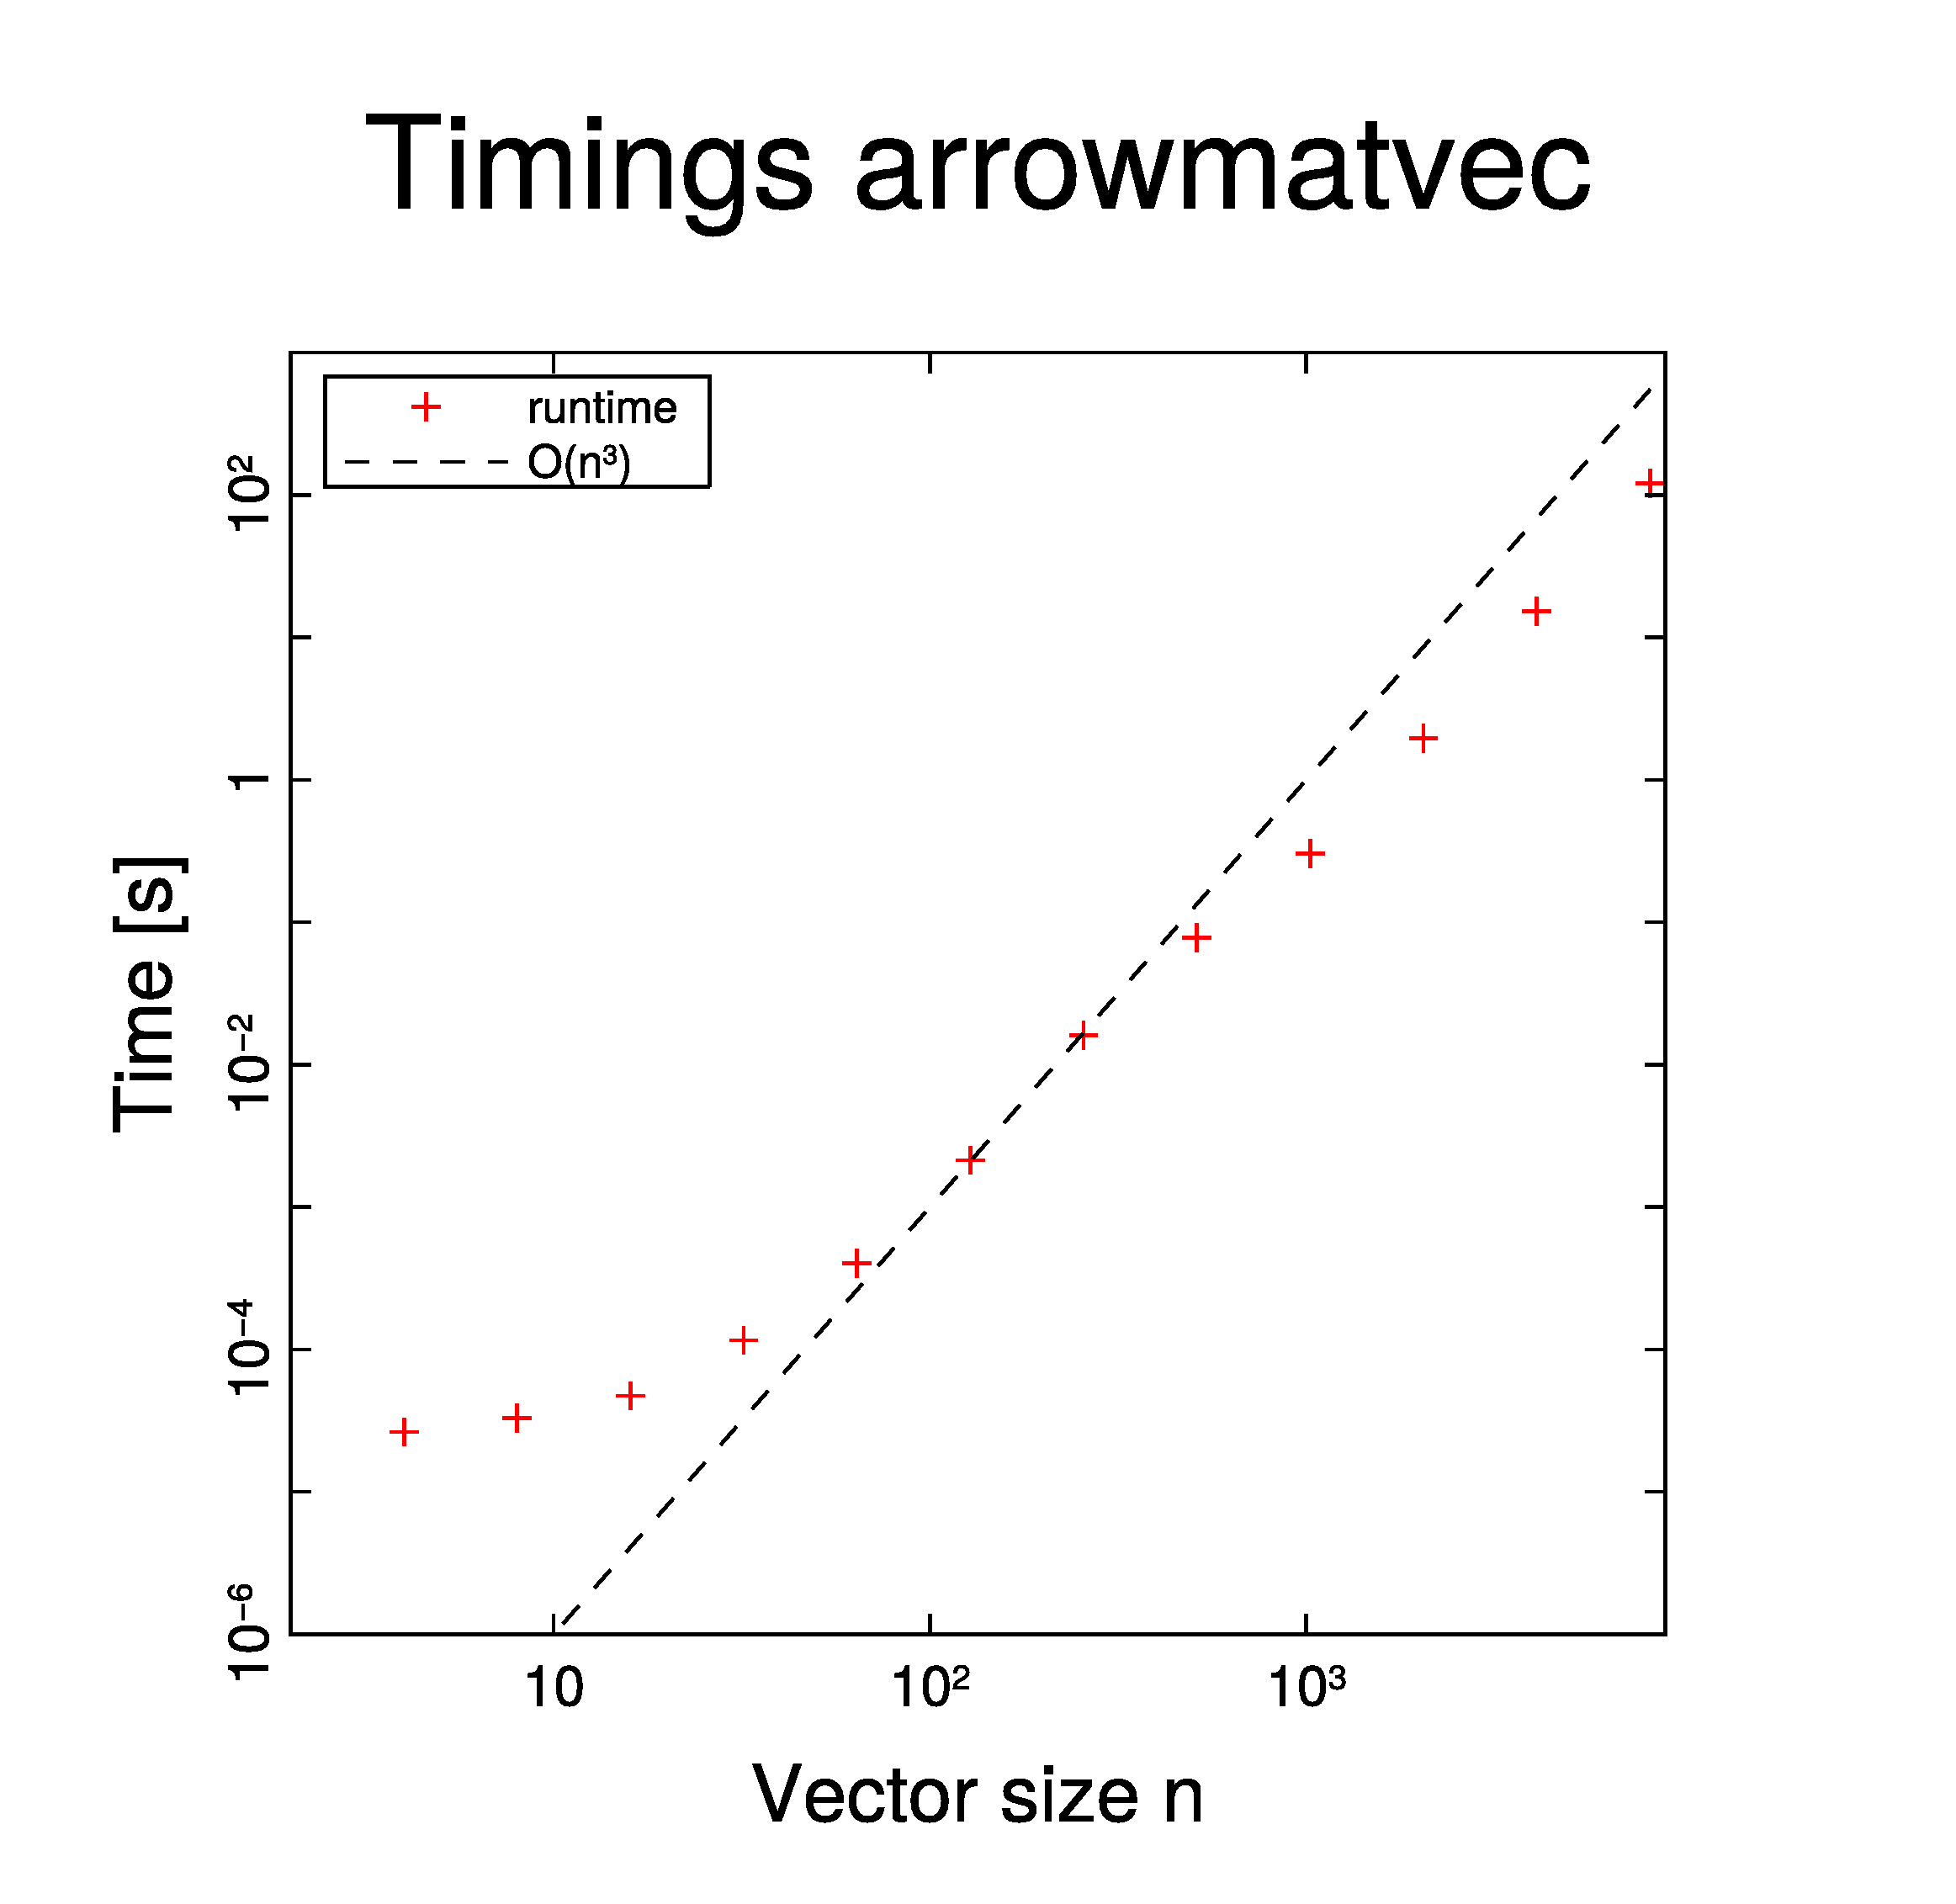
\includegraphics[width=0.8\textwidth]{\problems/\chpt/PICTURES/arrowmatvectiming.eps}
\caption{timings for \texttt{arrowmatvec(d,a,x)}}
\label{fig:arrowmatvectiming}
\end{figure}


\begin{hint}
This \Matlab~ created figure is provided as file
\texttt{arrowmatvectiming.\{eps,jpg\}}.
\end{hint}

\begin{solution}
The standard matrix-matrix multiplication has runtimes growing with $O(n^3)$ and the standard matrix-vector multiplication has runtimes growing with $O(n^2)$. Hence, the overall computational complexity is dominated by $O(n^3)$.
\end{solution}
\end{subproblem}

%%%%%%%%%%%% SUBPROBLEM 3

\begin{subproblem}[3]  \label{subprb:ArrowMatrixVector_3}
Write an \emph{efficient} \Matlab~ function 
\begin{center}
  \texttt{function y = arrowmatvec2(d,a,x)}
\end{center}
that computes the same multiplication as in code \ref{mc:ArrowMatrixVector_arrowmatvec} but with optimal asymptotic complexity with respect to {$n$}.
Here \texttt{d} passes the vector $(d_{1},\ldots,d_{n})^{T}$ and \texttt{a} passes the vector $(a_{1},\ldots,a_{n})^{T}$.

\begin{solution}
 Due to the sparsity and special structure of the matrix, it is possible to write a more efficient implementation than the standard matrix-vector multiplication. See code listing \ref{mc:ArrowMatrixVector_arrowmatvec2}
\vspace{0.5cm}

\lstinputlisting[caption={implementation of the function \texttt{arrowmatvec2}},label={mc:ArrowMatrixVector_arrowmatvec2}]
{\problems/\chpt/MATLAB/arrowmatvec2.m}
\end{solution}
\end{subproblem}

%%%%%%%%%%%% SUBPROBLEM 4

\begin{subproblem}[1]  \label{subprb:ArrowMatrixVector_4}
What is the complexity of your algorithm from sub-problem
\ref{subprb:ArrowMatrixVector_3} (with respect to problem size $n$)? 

\begin{solution}
The efficient implementation only needs two vector-vector element-wise multiplications and one vector-scalar multiplication. Therefore the complexity is $O(n)$.
\end{solution}
\end{subproblem}

%%%%%%%%%%%% SUBPROBLEM 5

\begin{subproblem}[2] \label{subprb:ArrowMatrixVector_5}
Compare the runtime of your implementation and the implementation given in code \ref{mc:ArrowMatrixVector_arrowmatvec} for $n=2^{5,6,\ldots,12}$.
Use the routines \texttt{tic} and \texttt{toc} as explained in example \ncseex{ex:effmatmult} of the Lecture Slides.

\begin{solution}
The standard matrix multiplication has runtimes growing with $O(n^3)$.
The runtimes of the more efficient implementation are growing with $O(n)$.
See \autoref{mc:ArrowMatrixVector_arrowmatvec2timing} and Figure~\ref{fig:arrowmatvec2timing}.

\lstinputlisting[caption={Execution and timings of \texttt{arrowmatvec} and \texttt{arrowmatvec2}}, label={mc:ArrowMatrixVector_arrowmatvec2timing}]
{\problems/\chpt/MATLAB/arrowmatvec2timing.m}

\begin{figure}[ht]
\centering
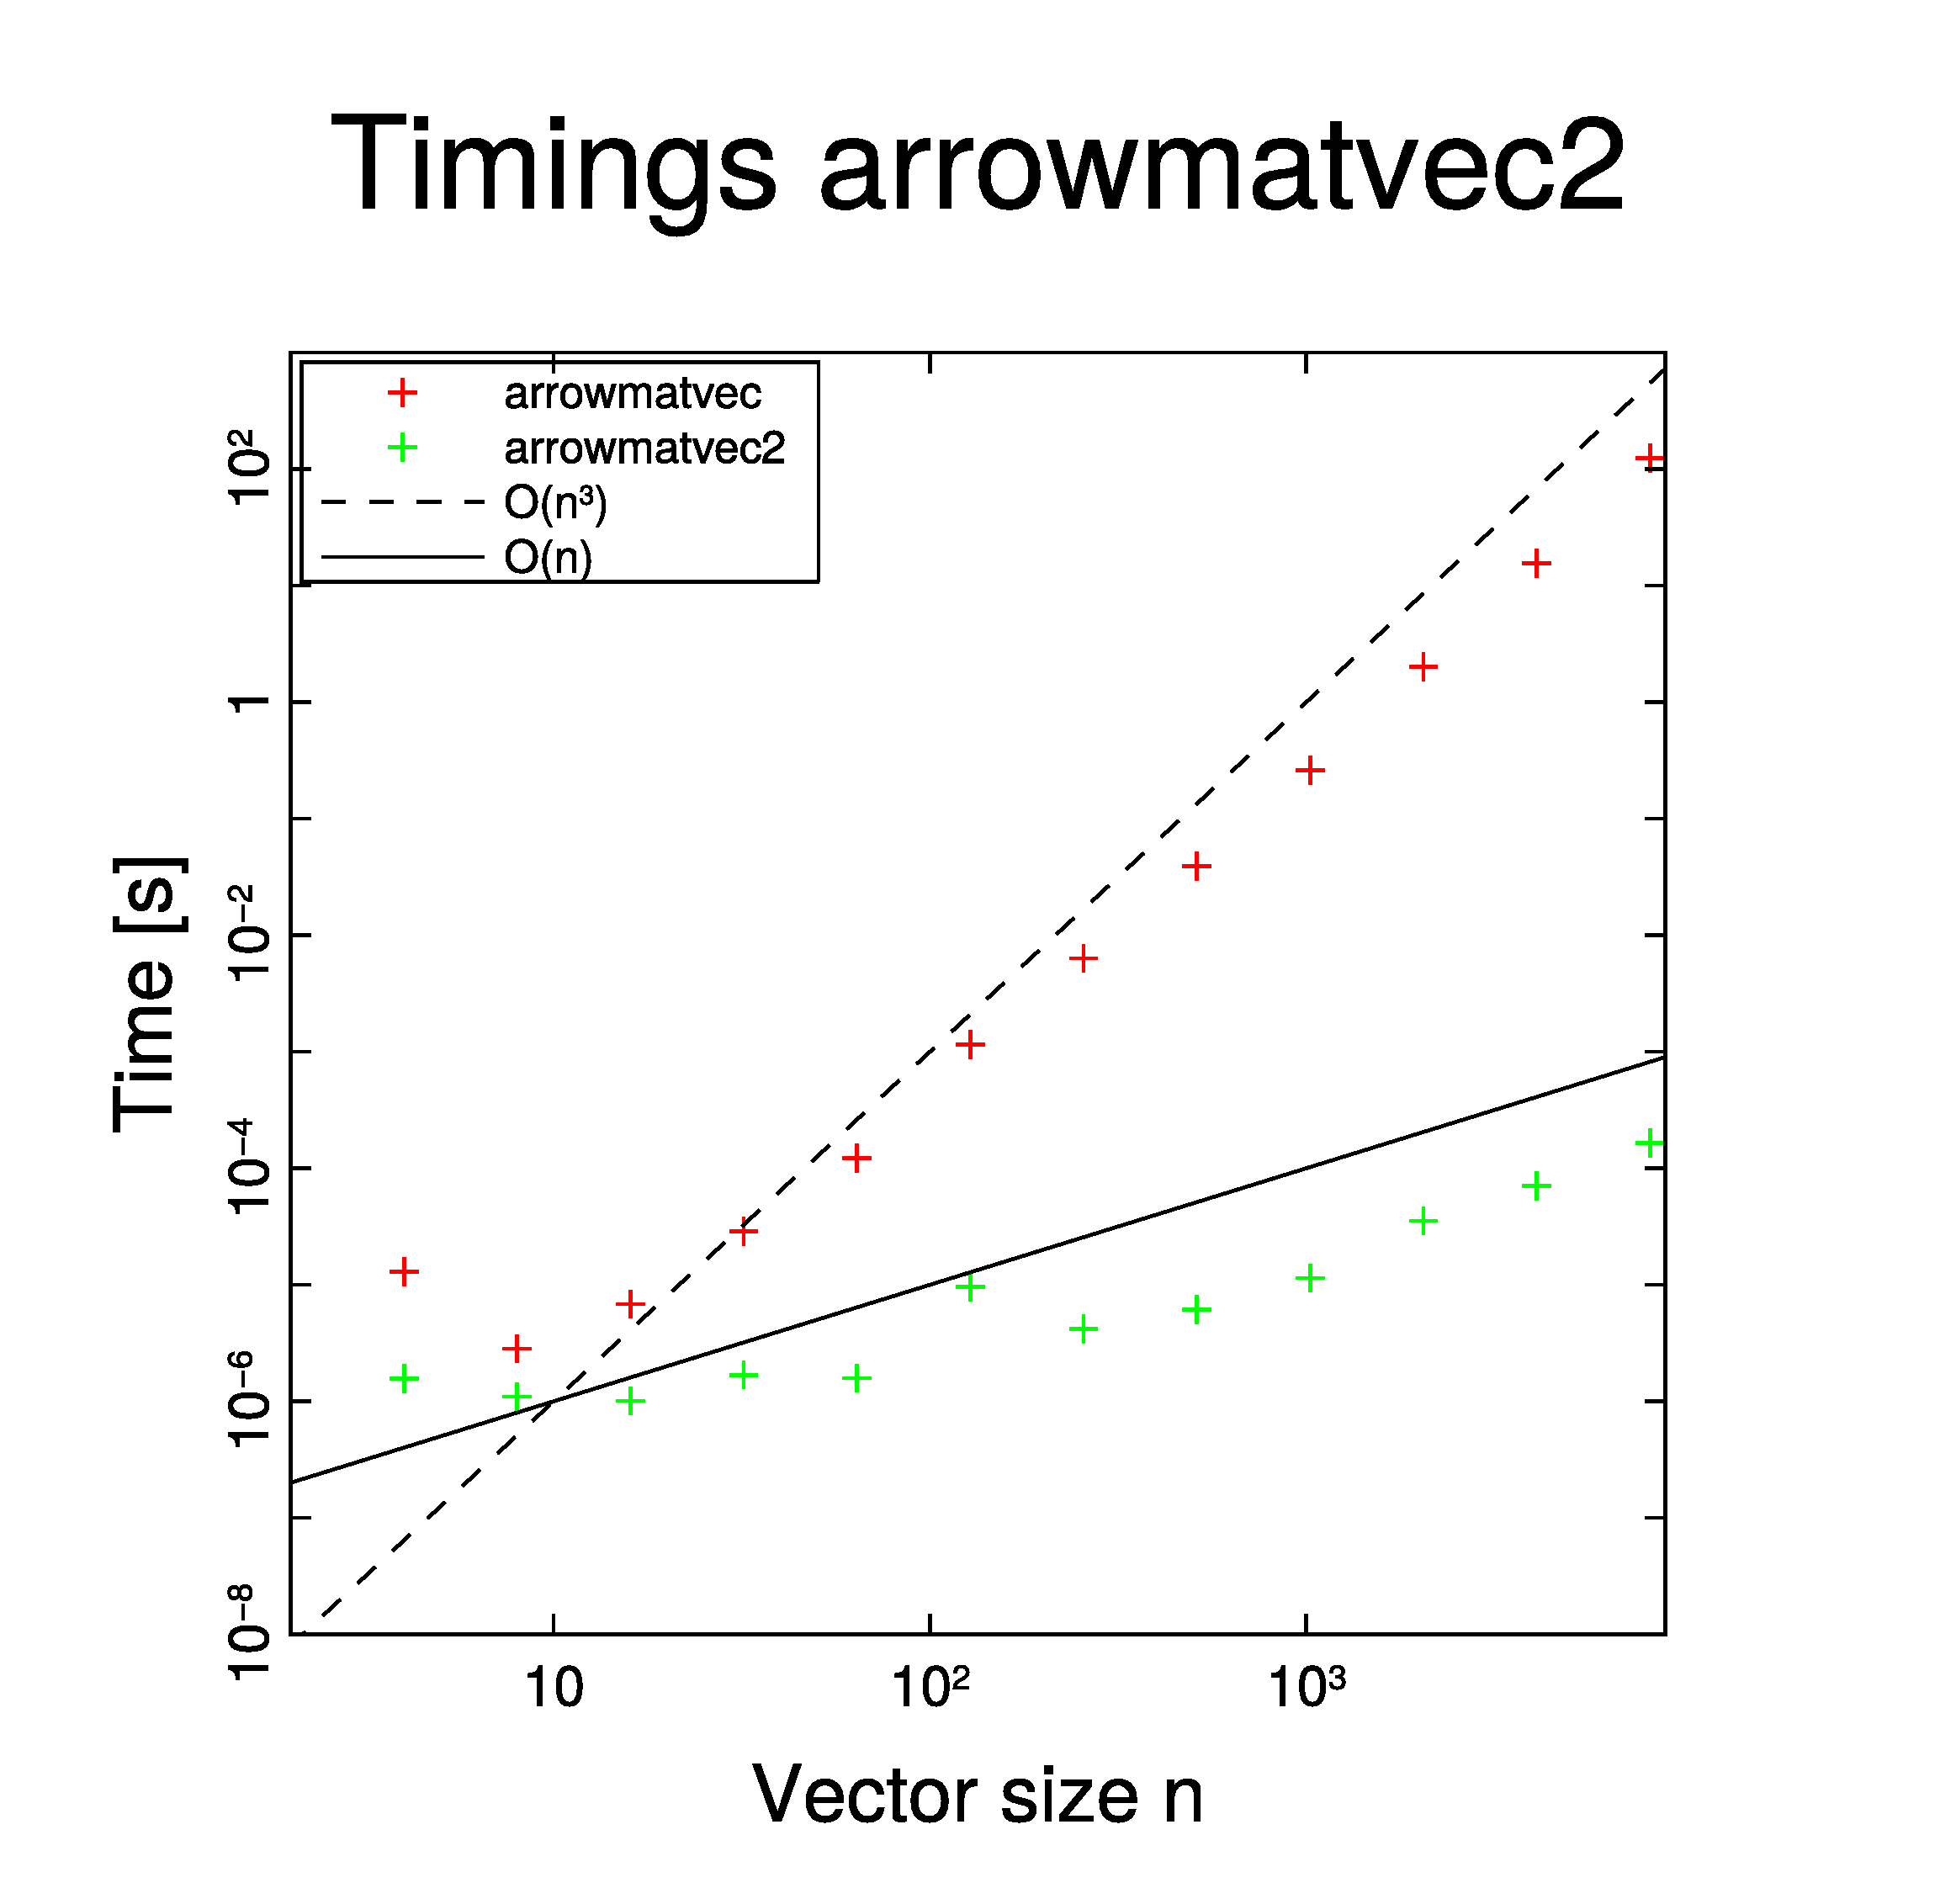
\includegraphics[width=0.8\textwidth]{\problems/\chpt/PICTURES/arrowmatvec2timing.eps}
\caption{timings for \texttt{arrowmatvec2(d,a,x)}} \label{fig:arrowmatvec2timing}
\end{figure}
\end{solution}
\end{subproblem}

\begin{subproblem}[1] \label{subprb:ArrowMatrixVector_6}
Write the \eigen{} codes corresponding to the functions \texttt{arrowmatvec} and \texttt{arrowmatvec2}.

\begin{solution}
See Listing~\ref{cppc:arrowmatvec} and Listing~\ref{cppc:arrowmatvec2}.

\lstinputlisting[style=cpp,caption={Implementation of \texttt{arrowmatvec}  in \eigen{}},label={cppc:arrowmatvec}]
{\problems/\chpt/CPP/arrowmatvec.cpp}

\lstinputlisting[style=cpp,caption={Implementation of \texttt{arrowmatvec2}  in \eigen{}},label={cppc:arrowmatvec2}]
{\problems/\chpt/CPP/arrowmatvec2.cpp}
\end{solution}
\end{subproblem}

\end{problem}
 %
% Required for hand-in: None
% Required for solution: PICTURES/error_cancellation.eps, MATLAB/cancellation.m

\renewcommand{\chpt}{ch_matvec}

\begin{problem}[Avoiding cancellation \coreproblem] \label{prb:cancellation}
  In \lref{sec:cancel} we saw that the so-called \emph{cancellation phenomenon} is
  a major cause of numerical instability, \emph{cf.} \lref{par:cancel}. Cancellation
  is the massive amplification of \emph{relative errors} when subtracting two
  real numbers of about the same value. 

  Fortunately, expressions vulnerable to cancellation can often be recast in
  a mathematically equivalent form that is no longer affected by cancellation,
  see \lref{par:cancelrem}. There we studied several examples, and this problem
  gives some more.

%  The following problems are taken from \cite[Chapter 2.5, pag. 35ff.]{Ascher}. For
%  additional exercises on the same subject, refer to the source.
 
 \begin{subproblem}[1]
   We consider the function
   \begin{gather}
     \label{eq:cancel:1}
     f_1(x_0,h) := \sin(x_0 + h) - \sin(x_0)\;.
   \end{gather}
   It  can the transformed into another form, $f_2(x_0,h)$, using the trigonometric identity
   \[
   \sin(\varphi) - \sin(\psi) = 2 \cos \left(\frac{\varphi + \psi}{2} \right) \sin \left(\frac{\varphi - \psi}{2} \right).
   \]
   Thus, $f_1$ and $f_2$ give the same values, in exact arithmetic, for any given argument values $x_0$ and $h$.
  
  \begin{enumerate}
   \item Derive $f_2(x_0,h)$, which does no longer involve the difference of
     return values of trigonometric functions.
   \item Suggest a formula that avoids cancellation errors for computing the
     approximation ($f(x_0 + h) - f(x_0)) / h$) of the derivative of
     $f(x) := \sin(x)$ at $x = x_0$. Write a \Matlab~ program that implements your
     formula and computes an approximation of $f'(1.2)$, for
     $h = 1 \cdot 10^{-20}, 1 \cdot 10^{-19},\cdots,1$.
     
     \begin{hint}
       For background information refer to \lref{ex:canceldiffq}.
     \end{hint}

   \item Plot the error (in doubly logarithmic scale using \matlab's
     \texttt{loglog} plotting function) of the derivative computed with the
     suggested formula and with the naive implementation using $f_1$.
   \item Explain the observed behaviour of the error.
  \end{enumerate}
  
  \begin{solution}
   Check the \Matlab{} implementation in \cref{mc:cancellation} and the plot in \cref{fig:error_cancellation}. We can clearly observe that the computation using $f_1$ leads to a big error as $h \rightarrow 0$. This is due to the cancellation error given by the subtraction of two number of approximately same magnitude. The second implementation using $f_2$ is very stable and does not display round-off errors.
   
   \lstinputlisting[language=matlab,caption={\Matlab{} script for \ref{prb:cancellation}},label={mc:cancellation}]{\problems/\chpt/MATLAB/cancellation.m}

    \begin{figure}[htb]
    \centering
    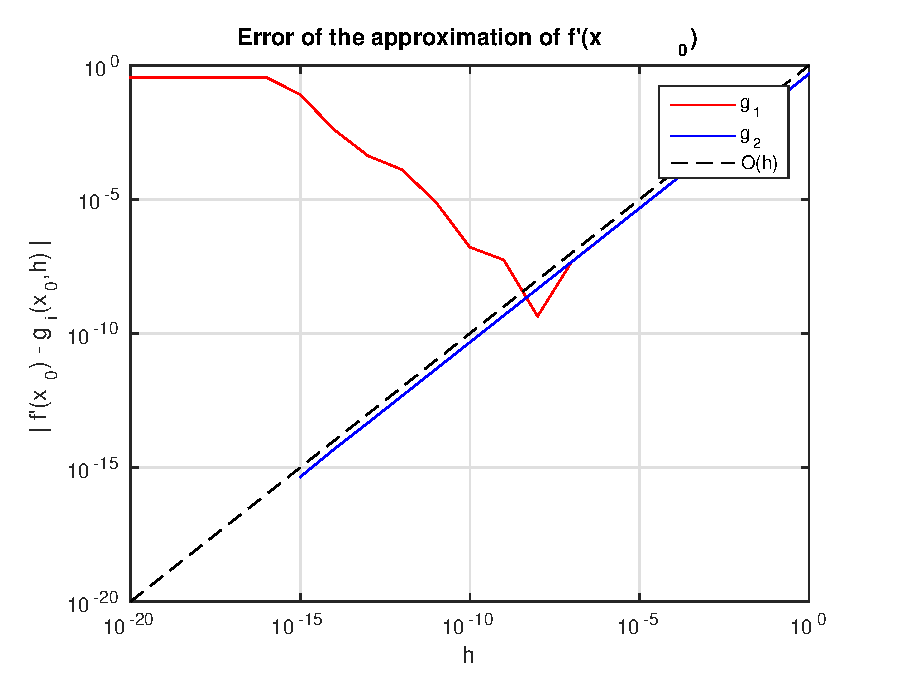
\includegraphics[width=0.8\textwidth]{\problems/\chpt/PICTURES/error_cancellation.eps}
    \caption{Timings for \ref{prb:cancellation}} \label{fig:error_cancellation}
    \end{figure}
  \end{solution}


 \end{subproblem}
 
 \begin{subproblem}[2]
   Using a trick applied in \lref{ex:canctrig} show that
  \begin{gather*}
    \ln(x - \sqrt{x^2 - 1}) = - \ln( x + \sqrt{x^2 - 1})\;.
  \end{gather*}
  Which of the two formulas is more suitable for numerical computation? Explain
  why, and provide a numerical example in which the difference in accuracy is
  evident.
   
  \begin{solution}
 We immediately derive $\ln(x - \sqrt{x^2 - 1}) + \ln(x + \sqrt{x^2 - 1}) = \log(x^2 - (x^2 - 1)) = 0$. As $x \rightarrow \infty$ the left $\log$ consists of subtraction of two numbers of equal magnitude, whilst the right $\log$ consists on the addition of two numbers of approximately the same magnitude. Therefore, in the first case there may be cancellation for large values of $x$, making it worse for numerical computation. Try, in \Matlab, with $x = 10^8$.
  \end{solution}

 \end{subproblem}

 \begin{subproblem}[2]
  For the following expressions, state the numerical difficulties that may occur, and rewrite the formulas in a way that is more suitable for numerical computation.
  \begin{enumerate}
   \item $\sqrt{x + \frac{1}{x}} - \sqrt{x - \frac{1}{x}}$, where $x \gg 1$.
   \item $\sqrt{\frac{1}{a^2} + \frac{1}{b^2}}$, where $a \approx 0, b \approx 1$.
  \end{enumerate}
  
  \begin{solution}
  \begin{enumerate}
   \item Inside the square roots we have the addition (rest. subtraction) of a small number to a big number. The difference of the square roots incur in cancellation, since they have the same, large magnitude. $A := x + \frac{1}{x}, B := x - \frac{1}{x}$ then $(A-B)(A+B)/(A+B) = \frac{2/x}{\sqrt{x + \frac{1}{x}} + \sqrt{x - \frac{1}{x}}} = \frac{2}{\sqrt{x} (\sqrt{x^2 + 1} + \sqrt{x^2 - 1})}$
   \item $\frac{1}{a^2}$ becomes very large as $a$ approaches $0$, whilst $\frac{1}{b^2} \rightarrow 1$ as $b \rightarrow 1$. Therefore, the relative size of $\frac{1}{a^2}$ and $\frac{1}{b^2}$ becomes so big, that, in computer arithmetic, $\frac{1}{a^2} + \frac{1}{b^2} = \frac{1}{a^2}$. On the other hand
   $\frac{1}{a}\sqrt{1+(\frac{a}{b})^{2}}$ avoids this problem by performing a division between two numbers with very different magnitude, instead of a summation.
  \end{enumerate}
  \end{solution}
 \end{subproblem}
\end{problem}
  %
% ncse_new/\problems/\chpt/ex_Kron.tex
% solutions require:    Kron_B.m     Kron_C.m     mainKron.m     kron_timings.eps

\renewcommand{\chpt}{ch_matvec}

\begin{problem}[Kronecker product] 
\label{prb:Kron}

In \lref{def:kron} we learned about the so-called Kronecker product, available
in \matlab{} through the command \texttt{kron}. In this problem we revisit the
discussion of \lref{ex:kron}. Please refresh yourself on this example and
study \lref{mc:kronmultv} again. 

As in \lref{ex:kron}, the starting point is the line of \matlab{} code
\begin{equation} \label{eq:ex_Kron}
  \mathbf{y}=\tt{kron(A,B)*x},
\end{equation} 
where the arguments are $\mathbf{A},\mathbf{B} \in \IR^{n,n}, \mathbf{x} \in \IR^{n \cdot n}$.

%%%%%%%%%%%% SUBPROBLEM 1

\begin{subproblem}[1] \label{subprb:Kron_1}
Obtain further information about the \texttt{kron} command from \Matlab~ help
issuing \texttt{doc kron} in the \matlab{} command window. 

\begin{solution}
See \Matlab~ help.
\end{solution}
\end{subproblem}

%%%%%%%%%%%% SUBPROBLEM 2

\begin{subproblem}[1] \label{subprb:Kron_2}
Explicitly write \cref{eq:ex_Kron}
in the form $\mathbf{y}=\mathbf{M} \mathbf{x}$ (i.e. write down $\vec{M}$), for
$\mathbf{A}=\begin{pmatrix}
         1 & 2   \\
         3 & 4   \\
 \end{pmatrix}$
and
$\mathbf{B}=\begin{pmatrix}
         5 & 6   \\
         7 & 8   \\
 \end{pmatrix}$.

\begin{solution}
$\Vy=\begin{pmatrix}
         5 & 6 & 10 & 12  \\
         7 & 8 & 14 & 16  \\
         15 & 18 & 20 & 24  \\
         21 & 24 & 28 & 32  \\
 \end{pmatrix}\Vx$.
\end{solution}
\end{subproblem}

%%%%%%%%%%%% SUBPROBLEM 3

\begin{subproblem}[1] \label{subprb:Kron_3}
What is the asymptotic complexity ($\to$ \lref{def:comp}) 
of the \Matlab~ code \eqref{eq:ex_Kron}? Use the Landau symbol
from \lref{def:O} to state your answer. 

\begin{solution}
\texttt{kron(A,B)} results in a matrix of size $n^2 \times n^2$ and $x$ has length $n^2$. So the complexity is the same as a matrix-vector multiplication for the resulting sizes. In total this is $O(n^2*n^2)=O(n^4)$.
\end{solution}
\end{subproblem}

%%%%%%%%%%%% SUBPROBLEM 4

\begin{subproblem}[2] \label{subprb:Kron_4} Measure the runtime of
  \eqref{eq:ex_Kron} for $n=2^{3,4,5,6}$ and random matrices. Use the \matlab{} functions
  \texttt{tic} and \texttt{toc} as explained in example \ncseex{ex:effmatmult} of
  the Lecture Slides.
  
 \begin{solution}
Since \texttt{kron(A,B)} creates a large matrix consisting of smaller blocks with size $n$, i.e. $B$ multiplied with $A(i,j)$, we can split the problem up in $n$ matrix-vector multiplications of size $n$. This results in a routine with complexity $n*O(n^2)=O(n^3)$ 
The implementation is listed in \ref{mc:Kron_B}.
The runtimes are shown in Figure~\ref{fig:kron_timings}.

\lstinputlisting[caption={An efficient implementation for \ref{prb:Kron}},label={mc:Kron_B}]
{\problems/\chpt/MATLAB/Kron_B.m}
 \end{solution}

\end{subproblem}

%%%%%%%%%%%% SUBPROBLEM 5

\begin{subproblem}[2] \label{subprb:Kron_5}
  Explain in detail, why \eqref{eq:ex_Kron} can be replaced with the single line
  of \matlab{} code
  \begin{gather}
    \label{eq:Kron:sl}
    \text{\texttt{y = reshape( B * reshape(x,n,n) * A', n*n, 1); }}
  \end{gather}
  and compare the execution times of \eqref{eq:ex_Kron} and \eqref{eq:Kron:sl} for
  random matrices of size $n=2^{3,4,5,6}$.
  
\begin{solution}
\lstinputlisting[caption={A second efficient implementation for \ref{prb:Kron} using \texttt{reshape}.},label={mc:Kron_C}]
{\problems/\chpt/MATLAB/Kron_C.m}
\lstinputlisting[caption={Main routine for runtime measurements of \ref{prb:Kron}},label={mc:mainKron}]
{\problems/\chpt/MATLAB/mainKron.m}

% \begin{figure}[htb]
% \centering
% 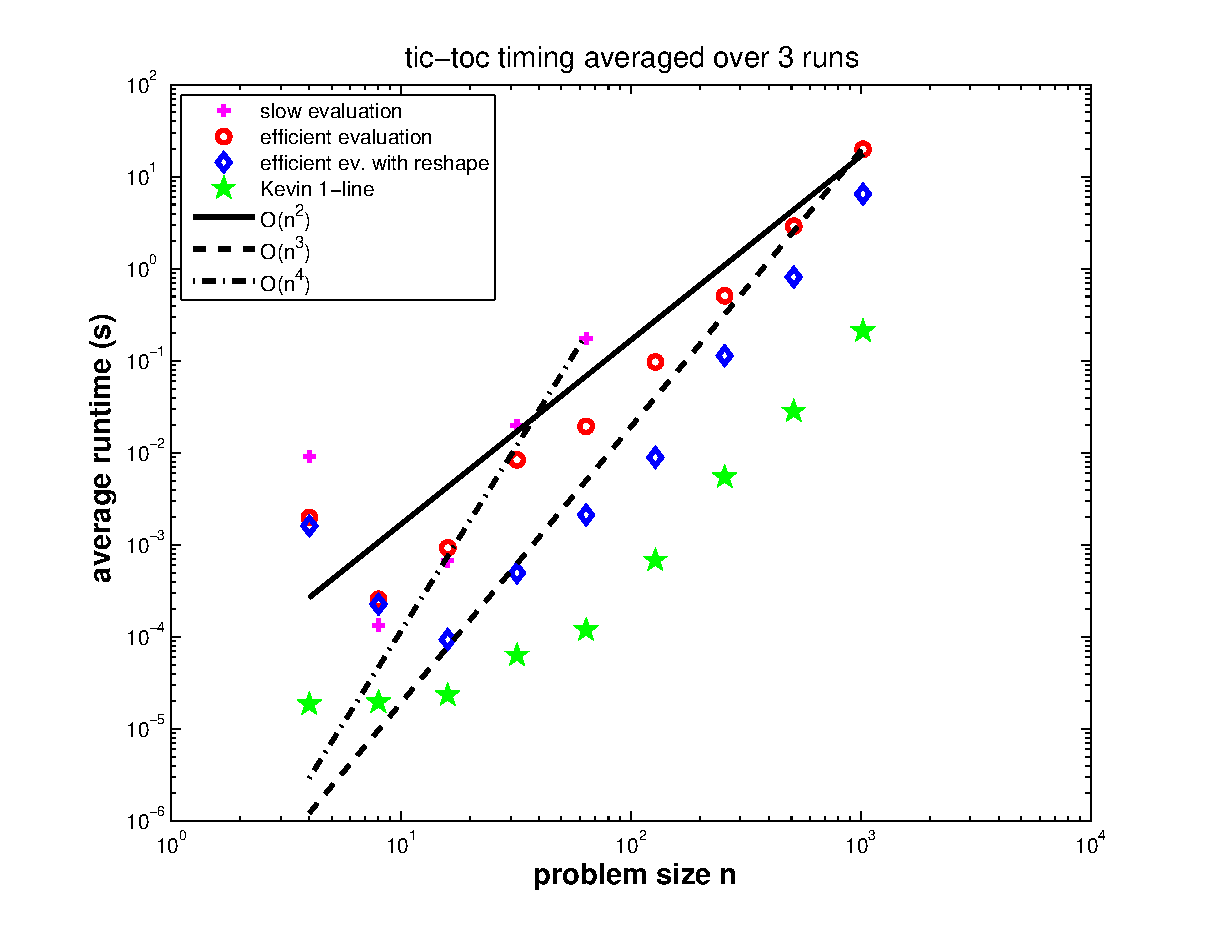
\includegraphics[width=0.8\textwidth]{\problems/\chpt/PICTURES/kron_timings.eps}
% \caption{Timings for \ref{prb:Kron}}\label{fig:kron_timings}
% \end{figure}
\end{solution}
\end{subproblem}

\begin{subproblem}[2] \label{subprb:Kron_6}
  Based on the \eigen{} numerical library ($\to$ \lref{sec:eigen}) implement a
  \Cpp{} function 
\begin{lstlisting}[style=cppsimple]
template <class Matrix>
void kron(const Matrix & A, const Matrix & B, Matrix & C) {
  // Your code here
}
\end{lstlisting}
returns the Kronecker product of the argument matrices \texttt{A} and \texttt{B}
in the matrix \texttt{C}. 

\begin{hint}
  Feel free (but not forced) to use the partial codes provided in \verb|kron.cpp| as well as the CMake file \verb|CMakeLists.txt| (including \verb|cmake-modules|) and the timing header file \verb|timer.h|~.
\end{hint}

\begin{solution}
    See \texttt{kron.cpp} or \cref{cppc:mainKron}.
\end{solution}
\end{subproblem}

\begin{subproblem}[2] \label{subprb:Kron_7}
  Devise an implementation of the \matlab{} code \eqref{eq:ex_Kron} in \Cpp according
  to the function definition
  \begin{lstlisting}[style=cppsimple]
template <class Matrix, class Vector>
void kron_mv(const Matrix & A, const Matrix & B, const Vector & x, Vector & y);
  \end{lstlisting}
  The meaning of the arguments should be self-explanatory. 

  \begin{solution}
    See \texttt{kron.cpp} or \cref{cppc:mainKron}.
  \end{solution}
\end{subproblem}

\begin{subproblem}[3] \label{subprb:kron:8}
  Now, using a function definition similar to that of the previous sub-problem,
  implement the \Cpp{} equivalent of \eqref{eq:Kron:sl} in the function
  \texttt{kron\_mv\_fast}. 

  \begin{hint}
    Study \lref{rem:eigrs} about ``reshaping'' matrices in \eigen{}.
  \end{hint}
\end{subproblem}

\begin{subproblem}[3] \label{subprb:kron:9}
  Compare the runtimes of your two implementations as you did for the \matlab{}
  implementations in sub-problem \ref{subprb:Kron_5}. 

\begin{solution}
\lstinputlisting[style=cpp,caption={Main routine for runtime measurements of \ref{prb:Kron}},label={cppc:mainKron}]
{\problems/\chpt/CPP/kron.cpp}

\begin{figure}[htb]
\centering
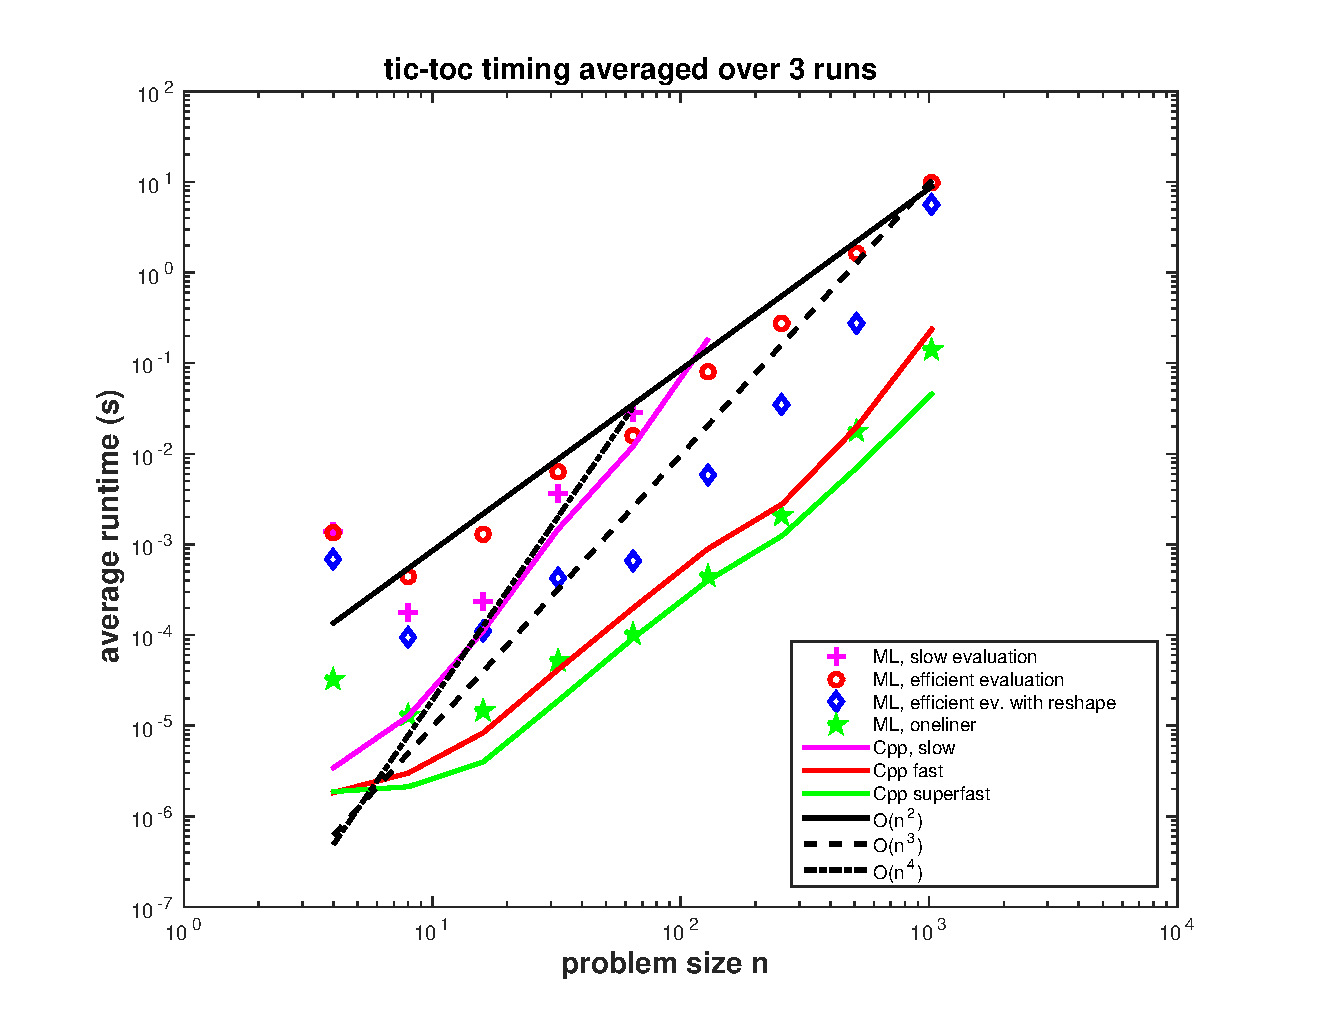
\includegraphics[width=0.8\textwidth]{\problems/\chpt/PICTURES/kron_timings_cpp.eps}
\caption{Timings for \ref{prb:Kron} with \Matlab and \Cpp implementations.} \label{fig:kron_timings}
\end{figure}
\end{solution}

\end{subproblem}

\end{problem} %
% ncse_new/\problems/\chptex_StructuredMatrixVector.tex
% the exercise requires:  multAB.m
% the solutions require:  multAmin.m , multAmin2.m
% R.H.: The last subproblem requires familiarity with the phenomenon of roundoff
% errors and cannot be posed in early stages of the course
\renewcommand{\chpt}{ch_matvec}

\begin{problem}[Structured matrix--vector product] 
  \label{prb:StructuredMatrixVector}

In \lref{ex:lrtrisum} we saw how the particular structure of a matrix can be
exploited to compute a matrix-vector product with substantially reduced
computational effort. This problem presents a similar case. 

Consider the real $n\times n$ matrix $\VA$ defined by $(\VA)_{i,j}=a_{i,j}=\min\{i,j\}$, for $i,j=1,\ldots,n$.
The matrix-vector product $\Vy=\VA\Vx$ can be implemented in \Matlab~ as
\begin{gather} \label{eq:structAx}
  \mathtt{ y = min(ones(n,1)*(1:n), (1:n)'*ones(1,n)) * x;}
\end{gather}

%%%%%%%%%%%% SUBPROBLEM 1
\begin{subproblem}[1] \label{subprb:StructuredMatrixVector_1}
What is the asymptotic complexity (for $n\to\infty$) of the evaluation of the \Matlab~ command displayed above, with respect to the problem size parameter $n$?

\begin{solution}
Matrix--vector multiplication:  quadratic dependence $O(n^2)$.
\end{solution}

\end{subproblem}

%%%%%%%%%%%% SUBPROBLEM 2
\begin{subproblem}[3] \label{subprb:StructuredMatrixVector_2}
%
Write an \emph{efficient} \Matlab~ function 
%
\begin{center}
\texttt{function y = multAmin(x)}
\end{center}
%
that computes the same multiplication as \eqref{eq:structAx} but with a better asymptotic complexity with respect to {$n$}.

\begin{hint}
you can test your implementation by comparing the returned values with the ones obtained with code \eqref{eq:structAx}.
\end{hint}

\begin{solution}
%
For every $j$ we have $y_j = \sum_{k=1}^j k x_k + j \sum_{k=j+1}^n x_k$, so we pre-compute the two terms for every $j$ only once.
%
\lstinputlisting[caption={implementation for the function multAmin},label={mc:StructuredMatrixVector_multAmin}]
{\problems/\chpt/MATLAB/multAmin.m}
\end{solution}

\end{subproblem}

%%%%%%%%%%%% SUBPROBLEM 3
\begin{subproblem}[1] \label{subprb:StructuredMatrixVector_3}
What is the asymptotic complexity (in terms of problem size parameter $n$) of your function \texttt{multAmin}?

\begin{solution}
Linear dependence: $O(n)$.
\end{solution}
%
\end{subproblem}

%%%%%%%%%%%% SUBPROBLEM 4

\begin{subproblem}[2] \label{subprb:StructuredMatrixVector_4}
Compare the runtime of your implementation and the implementation given in \eqref{eq:structAx} for $n=2^{5,6,\ldots,12}$.
Use the routines \texttt{tic} and \texttt{toc} as explained in example \ncseex{ex:effmatmult} of the Lecture Slides.

\begin{solution}
 
The matrix multiplication in \eqref{eq:structAx} has runtimes growing with $O(n^2)$.
The runtimes of the more efficient implementation with hand-coded loops, or using the \Matlab function \texttt{cumsum} are growing with $O(n)$.
%
\lstinputlisting[caption={comparison of execution timings}, label={mc:StructuredMatrixVector}]
{\problems/\chpt/MATLAB/multAmin_timings.m}
%
% \begin{figure}[ht]
% \centering
% \label{fig:multAmin_timings}
% \includegraphics[width=0.8\textwidth]{\problems/\chpt/PICTURES/multAmin_timings.eps}
% \caption{Timings for different implementations of $\Vy=\VA\Vx$}
% \end{figure}
% 
% \filippo{Decide wether to include next pic or not}

\begin{figure}[ht]
\centering
\label{fig:multAmin_timings}
\includegraphics[width=0.8\textwidth]{\problems/\chpt/PICTURES/multAmin_timings_cpp.eps}
\caption{Timings for different implementations of $\Vy=\VA\Vx$ with both \Matlab and \Cpp.}
\end{figure}

\end{solution}
\end{subproblem}

%%%%%%%%%%%% SUBPROBLEM 5
\begin{subproblem}[3] \label{subprb:StructuredMatrixVector_5}
Can you solve task \ref{subprb:StructuredMatrixVector_2} without using any \texttt{for}- or \texttt{while}-loop?\\
Implement it in the function
%
\begin{center}
\texttt{function y = multAmin2(x)}
\end{center}
%
\begin{hint}
 you may use the \Matlab built-in command \texttt{cumsum}.
\end{hint}

\begin{solution}
Using \texttt{cumsum} to avoid the \texttt{for} loops:
\lstinputlisting[caption={implementation for the function multAmin without loops},label={mc:StructuredMatrixVector_multAmin2}]
{\problems/\chpt/MATLAB/multAmin2.m}
\end{solution}
\end{subproblem}

%%%%%%%%%%%% SUBPROBLEM 6
\begin{subproblem}[1]  \label{subprb:StructuredMatrixVector_6}
 Consider the following \Matlab script \texttt{multAB.m}:
%
\lstinputlisting[caption={\Matlab script calling \texttt{multAmin}},label={mc:StructuredMatrixVector_multAB}]
{\problems/\chpt/MATLAB/multAB.m}
%
Sketch the matrix $\VB$ created in line 3 of \texttt{multAB.m}.

\begin{hint}
this \Matlab script is provided as file \texttt{multAB.m}.
\end{hint}

\begin{solution}
$$\VB:= \begin{pmatrix}
 2 & -1 &  0 & \cdots & 0 \\
-1 &  2 & -1 & \ddots & \vdots \\
 0 & \ddots & \ddots & \ddots & 0\\
\vdots & \ddots& -1 & 2 & -1\\
 0 & \cdots & 0 & -1 & 1
\end{pmatrix}$$
%
Notice the value 1 in the entry $(n,n)$.
\end{solution}
\end{subproblem}

%%%%%%%%%%%% SUBPROBLEM 7
\begin{subproblem}[2] \label{subprb:StructuredMatrixVector_7}
Run the code of
Listing~\ref{mc:StructuredMatrixVector_multAB} several times and conjecture a
relationship between the matrices $\VA$ and $\VB$ from the output. Prove your
conjecture.

\begin{hint}
You must take into account that computers inevitably commit round-off errors, see
\ncsesect{sec:marith}.
\end{hint}

\begin{solution}
It is easy to verify with \Matlab (or to prove) that $\VB=\VA^{-1}$.\\
For $2 \leq j \leq n-1$, we obtain:
%
\begin{equation*}
\begin{aligned}
(\VA\VB)_{i,j} &= \sum_{k=1}^n a_{i,k} b_{k,j}
= a_{i,j-1} b_{j-1,j} + 2 a_{i,j} b_{j,j} + a_{i,j+1} b_{j+1,j} \\
&= -\min(i,j-1) + 2 \min(i,j) - \min(i,j+1)
= \begin{cases}
-i + 2i - i = 0 & \text{ if } i<j, \\
-(i-1) + 2i - i = 1 & \text{ if } i=j, \\
-(j-1) + 2j - (j+1) = 0 & \text{ if } i>j.
\end{cases}
\end{aligned}
\end{equation*}
%
Furthermore, $(\VA\VB)_{i,1} = \delta_{i,1}$ and $(\VA\VB)_{i,n} = \delta_{i,n}$, hence $\VA\VB = {\bf I}$.\\
The last line of \texttt{multAB.m} prints the value of $\|\VA\,\VB\,\Vx-\Vx\|=\|\Vx-\Vx\|=0$.\\
The returned values are not exactly zero due to round-off errors.

\end{solution}
\end{subproblem}

\begin{subproblem}[2] \label{sp:smv:cpp1}
  Implement a \Cpp{} function with declaration
\begin{lstlisting}
template <class Vector>
void minmatmv(const Vector &x,Vector &y);    
\end{lstlisting}
that realizes the efficient version of the \matlab{} line of 
code \eqref{eq:structAx}. Test your function by comparing
with output from the equivalent \matlab{} functions. 

  \begin{solution}
    
 \lstinputlisting[caption={\Cpp script implementing \texttt{multAmin}},label={cppcc:StructuredMatrixVector_multAB}]
{\problems/\chpt/CPP/multAmin.cpp}
    
  \end{solution}
  
\end{subproblem}

\end{problem}

%Several runs of \texttt{multAB} from the previous sub-problem
%produced the following output:
%\begin{verbatim}
%>> multAB
%|x-y| = 3.587240e-15
%>> multAB
%|x-y| = 1.864381e-15
%>> multAB
%|x-y| = 5.324443e-16
%\end{verbatim}
%Explain these results.
%
%\hint: what is the relationship of the matrices $\VA$ and $\VB$?
%A fully rigorous proof is not required here.
 %
% ncse_new/\problems/\chpt/ex_Powers.tex
% solutions require:   Pow.m ,  mainPow.m,  Pow_timings.eps
\renewcommand{\chpt}{ch_matvec}

\begin{problem}[Matrix powers] \label{prb:Powers}

\begin{subproblem}[2] \label{subprb:Powers_1}
Implement a \Matlab~ function 
$$\mathtt{Pow(A,k)}$$
that, using only basic linear algebra operations (including matrix-vector or matrix-matrix multiplications), 
computes efficiently the $k^{th}$ power of the $n\times n$ matrix $\VA$.

\begin{hint}
 use the \Matlab~ operator $\wedge$ to test your implementation on random matrices $\VA$.
\end{hint}

\begin{hint}
 use the \Matlab~ functions \texttt{de2bi} to extract the ``binary digits'' of an integer. 
\end{hint}

\begin{solution}
Write $k$ in binary format: $k=\sum_{j=0}^M b_j\;2^j$,  $\:b_j\in\{0,1\}$. Then
$$\VA^k = \prod_{j=0}^M \VA^{2^j\; b_j} = \prod_{j\;s.t.\;b_j=1} \VA^{2^j}. $$
We compute $\VA,\;\VA^2,\;\VA^4,\;\ldots,\VA^{2^M}$ (one matrix-matrix multiplication each) and we multiply only the matrices $\VA^{2^j}$ such that $b_j\ne 0$.

\lstinputlisting[caption={An efficient implementation for \ref{prb:Powers}},label={mc:Pow}]
{\problems/\chpt/MATLAB/Pow.m}
\end{solution}
\end{subproblem}


%======================================================================================

\begin{subproblem}[1] \label{subprb:Powers_2}
Find the asymptotic complexity in $k$ (and $n$) taking into account that in \Matlab~ a matrix-matrix multiplication requires a $O(n^3)$ effort.

\begin{solution}
Using the simplest implementation:
$$A^k = \underbrace{\bigg(\ldots\Big(\big(A\cdot A\big)\cdot A\Big)\ldots \cdot A \bigg)\cdot A}_{k} \qquad \rightarrow \qquad O\big((k-1)n^3\big).$$
Using the efficient implementation from Listing~\ref{mc:Pow}, for each $j\in\{1,2,\ldots,\log_2(k)\}$
we have to perform at most two multiplications ($X*A$ and $A*A$):
$$ \text{complexity}\quad\leq \quad 2 * M * \text{matrix-matrix mult.} \quad \approx \quad 2 * \lceil\log_2 k\rceil * n^3.$$
($\lceil a\rceil = \mathtt{ceil}(a) =\inf\{ b\in\IZ,\; a\leq b\} $).
\end{solution}
\end{subproblem}


%======================================================================================

\begin{subproblem}[1] \label{subprb:Powers_3}
Plot the runtime of the built-in \Matlab~ power ($\wedge$) function and find out the complexity.
Compare it with the function \texttt{Pow} from \ref{subprb:Powers_1}.\\
Use the matrix
$$A_{j,k}= \frac1{\sqrt n} \;\exp\Big(\frac{2\pi i \;jk}n\Big)$$
to test the two functions.

\begin{solution}
\lstinputlisting[caption={Timing plots for \ref{prb:Powers}},label={mc:mainPow}]
{\problems/\chpt/MATLAB/mainPow.m}

\begin{figure}[htb]
\centering
\label{fig:Pow_timings}
\includegraphics[width=0.95\textwidth]{\problems/\chpt/PICTURES/Pow_timings.eps}
\caption{Timings for \ref{prb:Powers}}
\end{figure}

The \Matlab $\wedge$-function has (at most) logarithmic complexity in $k$ but the timing is slightly better than our implementation. % ~68\% on average

All the eigenvalues of the Vandermonde matrix $A$ have absolute value $1$, so the powers $A^k$ are ``stable'':
the eigenvalues of $A^k$ are not approaching neither $0$ nor $\infty$ when $k$ grows.
\end{solution}
\end{subproblem}

\begin{subproblem}[2] \label{sp:pow:o1}
  Using \eigen{}, devise a \Cpp{} function with the calling sequence
\begin{lstlisting}
template <class Matrix>
void matPow(const Matrix &A,unsigned int k);
\end{lstlisting}
that computes the $k^{\mathtt{th}}$ power of the square matrix $\VA$ (passed in
the argument \texttt{A}). Of course, your implementation should be as efficient
as the \matlab{} version from sub-problem \ref{subprb:Powers_1}.

\begin{hint}
 matrix multiplication suffers no aliasing issues (you can safely write \texttt{A = A*A}).
\end{hint}

\begin{hint}
 feel free to use the provided \func{matPow.cpp}.
\end{hint}

\begin{hint}
 you may want to use \texttt{log} and \texttt{ceil}.
\end{hint}

\begin{hint}
 \Eigen~ implementation of power (\texttt{A.pow(k)}) can be found in:
 \begin{verbatim}
  #include <unsupported/Eigen/MatrixFunctions>
 \end{verbatim}
\end{hint}

\begin{solution}
\lstinputlisting[caption={Implementation of \func{matPow}},label={cppc:matPow}]
{\problems/\chpt/CPP/matPow.cpp}
\end{solution}
\end{subproblem}
\end{problem}
 %
% Required for hand-in: getit.m
% Required for solution: None

\begin{problem}[Complexity of a \Matlab~ function] \label{prb:lineariter} 
In this problem we recall a concept from linear algebra, the diagonalization
of a square matrix. Unless you can still define what this means, please look
up the chapter on ``eigenvalues'' in your linear algebra lecture notes. This
problem also has a subtle relationship with \ref{prb:Powers}

We consider the \Matlab~ function defined in \verb|getit.m|~ (cf. \cref{mc:lineariter})
\lstinputlisting[language=matlab,caption={\Matlab implementation of \func{getit} for \ref{prb:lineariter}.},label={mc:lineariter}]
{\problems/\chpt/MATLAB/getit.m}

\begin{hint}
  Give the command \func{doc eig} in \Matlab{} to understand what \texttt{eig}
  does. 
\end{hint}

\begin{hint}
  You may use that \texttt{eig} applied to an $n\times n$-matrix requires an
  asymptotic computational effort of $O(n^{3})$ for $n\to\infty$.
\end{hint}

\begin{hint}
 in \Matlab, the function \func{diag(x)} for $\vec{x} \in \mathbb{R}^n$, builds a diagonal, $n \times n$ matrix with $\vec{x}$ as diagonal. If $\vec{M}$ is a $n \times n$ matrix, \func{diag(M)} returns (extracts) the diagonal of $\vec{M}$ as a vector in $\mathbb{R}^n$.
\end{hint}

\begin{hint}
 the operator \verb|v.^k| for $v \in \mathbb{R}^n$ and $k \in \mathbb{N} \setminus \{ 0 \}$ returns the vector with components $v_i ^k$ (i.e. component-wise exponent)
\end{hint}

\begin{subproblem}[2]
 What is the output of \func{getit}, when $A$ is a diagonalizable $n \times n$ matrix, $x \in \mathbb{R}^n$ and $k \in \mathbb{N}$?
 
 \begin{solution}
   The output is $\vec{y}$ s.t. $\vec{y} = \vec{A}^k \vec{x}$. The eigenvalue decomposition of the matrix $\vec{A} = \vec{S} \vec{D} \vec{S}^{-1}$ (where $\vec{D}$ is diagonal and $\vec{S}$ invertible), allows us to write:
   \[
    \vec{A}^k = (\vec{S} \vec{D} \vec{S}^{-1})^k = \vec{S} \vec{D}^k \vec{S}^{-1},
   \]
   and $\vec{D}^k$ can be computed efficiently (component-wise) for diagonal matrices.
 \end{solution}

\end{subproblem}

\begin{subproblem}[1]
  Fix $k \in \mathbb{N}$. Discuss (in detail) the asymptotic complexity of
  \func{getit} $n\to\infty$.
 
 \begin{solution}
  The algorithm comprises the following operations:
  \begin{itemize}
   \item diagonalization of a full-rank matrix $\vec{A}$ is $O(n^3)$;
   \item matrix-vector multiplication is $O(n^2)$;
   \item raising a vector in $\mathbb{R}^n$ for the power $k$ has complexity $O(n)$;
   \item solve a fully determined linear system: $O(n^3)$.
  \end{itemize}
  The complexity of the algorithm is dominated by the operations with higher exponent. Therefore the total complexity of the algorithm is $O(n^3)$ for $n \rightarrow \infty$.
 \end{solution}
\end{subproblem}

\end{problem}
 %
\end{sheet}

%%% PS2
\begin{sheet}{2}{24.09.2015}{01.10.2015}
You should try to your best to do the core problems. If time permits, please try to do the rest as well.
% ncse_new/p1_SystemsOfEquations/ch2_DirectMethodsLSE/ex_Lyapunov.tex
% solutions require:  solveLyapunov.m



\begin{problem}[Lyapunov Equation \coreproblem]\label{prb:Lyapunov}

  Any linear system of equations with a finite number of unknowns can be written in the
  ``canonical form'' $\VA\Vx=\Vb$ with a system matrix $\VA$ and a right hand side
  vector $\Vb$. However, the LSE may be given in a different form and it may not be
  obvious how to extract the system matrix. This task gives an intriguing example
  and also presents an important \emph{matrix equation}, the so-called
  \href{http://en.wikipedia.org/wiki/Lyapunov_equation}{Lyapunov Equation}. 

  Given $\mathbf{A}\in \mathbb{R}^{n\times n}$, consider the equation
  \begin{equation}
    \label{eq:Lyapunov}
    \VA\VX + \VX\VA^{T} = \VI
  \end{equation}
  with unknown $\mathbf{X}\in\mathbb{R}^{n\times n}$.

\begin{subproblem}[1]\label{lpy:sp:0}
Show that for a fixed matrix $\VA\in\bbR^{n,n}$ the mapping 
\begin{gather*}
  L: \left\{
    \begin{array}[c]{ccl}
      \bbR^{n,n} & \to & \bbR^{n,n} \\
      \VX & \mapsto & \VA\VX + \VX\VA^{T}
    \end{array}\right.
\end{gather*}
is linear.

\begin{hint}
  Recall from linear algebra the definition of a linear mapping between two vector spaces.
\end{hint}
  \begin{solution}
  Take $\alpha,\beta\in\R$ and $\VX,\VY\in\bbR^{n,n}$. We readily compute
  \[
  \begin{split}
  L(\alpha \VX+\beta \VY)&=A(\alpha \VX+\beta \VY)+(\alpha \VX+\beta \VY)A^T\\
  &=\alpha A \VX+\beta A \VY+\alpha \VX A^T +\beta \VY A^T\\
  &=\alpha (A \VX+\VX A^T)+\beta( A \VY+ \VY A^T)\\
  &=\alpha L(\VX)+\beta L(\VY),
  \end{split}
  \]
  as desired.
  \end{solution}
\end{subproblem}

In the sequel let ${\rm vec}(\vec{M})\in\R^{n^2}$ denote the column vector
obtained by reinterpreting the internal coefficient array of a matrix
$M\in\R^{n,n}$ stored in column major format as the data array of a vector with
$n^2$ components. In MATLAB, ${\rm vec}(\vec{M})$ would be the column vector
obtained by \texttt{reshape(M,n*n,1)} or by \texttt{M(:)}. See \lref{rem:eigrs}
for the implementation with Eigen.

Problem \eqref{eq:Lyapunov} is equivalent to a linear system of equations
  \begin{equation}
    \label{eq:systemLyapunov}
   \VC{\rm vec}(\VX)=\Vb
  \end{equation}
with system matrix $\VC\in\R^{n^2,n^2}$ and right hand side vector $\Vb\in\R^{n^2}$.

\begin{subproblem}[1]\label{lpy:sp:0a}
  Refresh yourself on the notion of ``sparse matrix'', see \lref{sec:sparse} and,
  in particular, \lref{def:sparse}, \lref{def:sparse2}. 
\end{subproblem}

\begin{subproblem}[1]
Determine $\VC$ and $\Vb$ from \eqref{eq:systemLyapunov} for $n=2$ and
\[
\VA=\begin{bmatrix}
2 & 1 \\ -1 & 3
\end{bmatrix}.
\]

\begin{solution}
Write $X=\left[ \begin{smallmatrix} x_1 & x_3 \\ x_2 & x_4 \end{smallmatrix} \right]$, so that ${\rm vec}(\VX)=(x_i)_i$. A direct calculation shows that \eqref{eq:Lyapunov} is equivalent to \eqref{eq:systemLyapunov} with
\[
\VC=
\begin{bmatrix}
4 & 1 & 1 & 0 \\
-1 & 5 & 0 & 1 \\
-1 & 0 & 5 & 1\\
0 & -1 & -1 & 6
\end{bmatrix} 
\;\text{and}\;
\Vb=
\begin{bmatrix}
1 \\
0 \\
0\\
1
\end{bmatrix}.
\]
\end{solution}
\end{subproblem}

\begin{subproblem}[3]
Use the Kronecker product to find a general expression for $\VC$ in terms of a general $\VA$.
\begin{solution}
We have $\VC=\mathbf{I}\bigotimes
  \mathbf{A}+\mathbf{A}\bigotimes \mathbf{I}$. The first term is related to
  $\VA\VX$, the second to $\VX\VA^{T}$. 
\end{solution}
\end{subproblem}

\begin{subproblem}[2]
Write a \Matlab~ function 
\begin{center}
  \texttt{function C = buildC (A)}
\end{center}
that returns the matrix $\VC$ from \eqref{eq:systemLyapunov} when given a square matrix $\VA$. (The function \texttt{kron} may be used.)
\begin{solution}
See Listing~\ref{mc:Lyapunov}.
\lstinputlisting[caption={Building the matrix $\VC$ in \eqref{eq:systemLyapunov} with MATLAB}, label={mc:Lyapunov}]{\problems/ch_directmethodslse/MATLAB/buildC.m}

%The use of \texttt{speye} makes the matrix \texttt{B} and the right-hand side
%\texttt{b} sparse, the result is faster and more accurate (check the residual
%$\|\VA\VX-\VX\VA^T-\VI\|$). 


\end{solution}
\end{subproblem}

\begin{subproblem}[4]
Give an upper bound (as sharp as possible) for ${\rm nnz}(\VC)$ in terms of ${\rm nnz}(\VA)$. Can $\VC$ be legitimately regarded as a sparse matrix for large $n$ even if $\VA$ is dense?
\begin{hint}
Run the following MATLAB code:

\texttt{n=4; \\
A=sym('A',[n,n]); \\
I=eye(n); \\
C=buildC(A)}
\end{hint}
\begin{solution}
%The block in position $(i,j)$ of the matrix $\VC$ is given by $a_{ij}I+\delta_{ij}A$. Suppose now that $a_{ij}\neq 0$. We have two cases:
%\begin{itemize}
%\item Case $i\neq j$. This gives at most $n$ non-zero entries in the block in position $(i,j)$ of the matrix $\VC$, which is equal to $a_{ij}I$, and one non-zero entry in each diagonal block. This gives a total of, at most, $2n$ non-zero entries.
%\item Case $i=j$. This gives at most one non-zero entry in each diagonal block, thus a total of, at most, $n$ non-zero entries.
%\end{itemize}
Note that, for general matrices $\VA$ and $\VB$ we have ${\rm nnz}(\VA\otimes \VB)={\rm nnz}(\VA){\rm nnz}(\VB)$. This follows from the fact that the block in position $(i,j)$ of the matrix $\VA\otimes \VB$ is $a_{ij}\VB$. In our case, we immediately obtain
\[
{\rm nnz}(\VC)={\rm nnz}(\mathbf{I}\otimes
  \mathbf{A}+\mathbf{A}\otimes \mathbf{I})\le {\rm nnz}(\mathbf{I}\otimes
  \mathbf{A}) +{\rm nnz}(\mathbf{A}\otimes \mathbf{I})\le 2 {\rm nnz}(\VI){\rm nnz}(\VA),
\]
namely
\[
{\rm nnz}(\VC)\le 2n {\rm nnz}(\VA).
\]
The optimality of this bound can be checked by taking the matrix $\VA=\left[ \begin{smallmatrix} 0 & 1 \\ 1 & 0 \end{smallmatrix} \right]$.

This bound says that, in general, even if $\VA$ is not sparse, we have  ${\rm nnz}(\VA)\le 2 n^3 \ll n^4$. Therefore, $\VC$ can be regarded as a sparse matrix for any $\VA$.
\end{solution}
\end{subproblem}

\begin{subproblem}[3]
Implement a C++ function

\texttt{Eigen::SparseMatrix<double> buildC(const MatrixXd \&A)}

that builds the Eigen matrix $\VC$ from $\VA$. Make sure that initialization is done efficiently using an intermediate triplet format. Read \ncserem{sec:eigensparse} very carefully before starting.
\begin{solution}
See \texttt{solveLyapunov.cpp}.
\end{solution}
\end{subproblem}

\begin{subproblem}[1]\label{subprob:12345}
Validate the correctness of your C++ implementation of \texttt{buildC} by comparing with the equivalent Matlab function for $n=5$ and
\[
A=\begin{bmatrix}
10 & 2 & 3 & 4 & 5 \\
6 & 20 & 8 & 9 & 1\\
1 & 2 & 30 & 4 & 5 \\
6 & 7 & 8 & 20 & 0\\
1 & 2 & 3 & 4 & 10
\end{bmatrix}.
\]
\begin{solution}
See \texttt{solveLyapunov.cpp}  and \texttt{solveLyapunov.m}.
\end{solution}
\end{subproblem}

\begin{subproblem}[2]
Write a C++ function

\texttt{void solveLyapunov(const MatrixXd \& A, MatrixXd \& X)}

that returns the solution of \eqref{eq:Lyapunov} in the $n\times n$-matrix $\VX$, if $A\in \R^{n,n}$.
\begin{solution}
See \texttt{solveLyapunov.cpp}.

\emph{Remark.} Not every invertible matrix $\VA$ allows a solution: if $\VA$ and
$-\VA$ have a common eigenvalue the system $\VC\Vx=\Vb$ is singular, try it with
the matrix $\VA=\begin{bmatrix}0 &1\\1 & 0\end{bmatrix}$. For a more efficient
solution of the task, see Chapter 15 of Higham's book.
\end{solution}
\end{subproblem}

\begin{subproblem}[2]
Test your C++ implementation of \texttt{solveLyapunov} by comparing with Matlab for the test case proposed in \ref{subprob:12345}.

\begin{solution}
See \texttt{solveLyapunov.cpp} and \texttt{solveLyapunov.m}.
\end{solution}
\end{subproblem}
\end{problem}
 %
% ncse_new/p1_SystemsOfEquations/ch2_DirectMethodsLSE/ex_PartitionedMatrix.tex
% solutions require:  solvelse.m

\begin{problem}[Partitioned Matrix \coreproblem] \label{prb:PartitionedMatrix}

Based on the block view of matrix multiplication presented in \lref{rem:blockops},
we looked a \emph{block elimination} for the solution of block partitioned linear
systems of equations in \lref{par:belim}. Also of interest are \lref{rem:BlockLU} and
\lref{rem:partlu} where LU-factorization is viewed from a block perspective. 
Closely related to this problem is \lref{ex:arrowlse}, which you should study
again as warm-up to this problem. 

Let the matrix $\VA\in\bbR^{n+1,n+1}$ be partitioned according to
\begin{align} \label{eq:block_matrix_lu}
\mathbf{A}=\left[
    \begin{array}{ccccccc}
      \mathbf{R}&\Vv\\
      \Vu^{T}&0
    \end{array}\right]\;,
\end{align}
where $\Vv\in\mathbb{R}^{n}$, $\Vu\in\mathbb{R}^{n}$, and
$\mathbf{R}\in\mathbb{R}^{n\times n}$ is \underline{upper triangular} and \underline{regular}.

\begin{subproblem}[1] \label{subprb:PartitionedMatrix_a}
  Give a necessary and sufficient condition for the triangular matrix $\vec{R}$ to be invertible.
  
  \begin{solution}
   $\vec{R}$ being upper triangular $\det (\vec{R}) = \prod_{i = 0}^n (\vec{R})_{i,i}$, means that all the diagonal elements must be non-zero for $\vec{R}$ to be invertible.
  \end{solution}

\end{subproblem}

\begin{subproblem}[2] \label{subprb:PartitionedMatrix_b}
  Determine expressions for the subvectors $\vec{z} \in \IR^n, \xi \in \IR$ of the solution vector of the linear system of equations
  \begin{align*}
   \begin{bmatrix}
      \mathbf{R} & \Vv\\
      \Vu^{T}  & 0 
   \end{bmatrix} \begin{bmatrix} \vec{z} \\ \xi \end{bmatrix} = \begin{bmatrix} \vec{b} \\ \beta \end{bmatrix}
  \end{align*}
  for arbitrary $\vec{b} \in \IR^n, \beta \in \IR$.

  \begin{hint}
   Use blockwise Gaussian elimination as presented in \lref{par:belim}. 
  \end{hint}


\begin{solution}
% Find the $\mathtt{LU}$-decomposition of $\mathbf{A}$.
% The $\mathtt{LU}$-decomposition is
% $$\mathbf{A}=\mathbf{LU}=\left(
%     \begin{array}{ccccccc}
%       \mathbf{I}&0\\
%       \Vu^{T}\mathbf{R}^{-1}&1
%     \end{array}\right)\left(
%     \begin{array}{ccccccc}
%       \mathbf{R}&\Vv\\
%  0&-\mathbf{u}^{T}\mathbf{R}^{-1}\mathbf{v}
%     \end{array}\right)$$
Applying the computation in \lref{rem:blockgs}, we obtain:
  \begin{align*}
   \begin{bmatrix}
      \vec{1} & 0 \\
      0  & 1
   \end{bmatrix} \begin{bmatrix} \vec{z} \\ \xi \end{bmatrix} = \begin{bmatrix}
   \vec{R}^{-1} ( \vec{b} - \vec{v} s^{-1} b_s )\\
   s^{-1} b_s
   \end{bmatrix}
  \end{align*}
    with $s := - (\vec{u}^\top \vec{R}^{-1} \vec{v}), b_{s} := (\beta - \vec{u}^\top \vec{R}^{-1} \vec{b})$.
\end{solution}
\end{subproblem}

\begin{subproblem}[2]
  Show that $\mathbf{A}$ is regular if and only if $\Vu^{T}\mathbf{R}^{-1}\Vv\neq0$.
  \begin{solution}
    The square matrix $\VA$ is regular, if the corresponding linear system has a
    solution for every right hand side vector. If $\Vu^{T}\mathbf{R}^{-1}\Vv\neq0$
    the expressions derived in the previous sub-problem show that a solution
    can be found for any $\Vb$ and $\beta$, because $\VR$ is already known to be
    invertible.
  \end{solution}
\end{subproblem}
  
\begin{subproblem}[3]
\label{subprb:PartitionedMatrix_d}
Implement the \Cpp{} function
\begin{lstlisting}[style=cppsimple]
 template <class Matrix, class Vector>
 void solvelse(const Matrix & R, const Vector & v, const Vector & u, const Vector & b, Vector & x);
\end{lstlisting}
for computing the solution of $\vec{A}\Vx=\Vb$ (with $\vec{A}$ as in 
\eqref{eq:block_matrix_lu}) efficiently. Perform size check on input matrices and vectors. 

\begin{hint}
 Use the decomposition from \ref{subprb:PartitionedMatrix_b}.
\end{hint}

\begin{hint}
 you can rely on the \verb|triangularView()| function to instruct \Eigen{} of the
 triangular structure of $\vec{R}$, see \lref{cpp:blockOps}. 
\end{hint}

\begin{hint}
 using the construct:
\begin{lstlisting}[style=cppsimple]
    typedef typename Matrix::Scalar Scalar; 
\end{lstlisting}
you can obtain the scalar type of the \verb|Matrix| type (e.g. \verb|double| for \verb|MatrixXd|). This can then be used as:
\begin{lstlisting}[style=cppsimple]
 Scalar a = 5;
\end{lstlisting}
\end{hint}

\begin{hint}
 using \verb|triangularView| and templates you may incur in weird compiling errors. If this happens to you, check \href{http://eigen.tuxfamily.org/dox/TopicTemplateKeyword.html}{http://eigen.tuxfamily.org/dox/TopicTemplateKeyword.html}
\end{hint}

\begin{hint}
 sometimes the C++ keyword \verb|auto| (only in std. C++11) can be used if you do not want to explicitly write the return type of a function, as in:
\begin{lstlisting}[style=cppsimple]
 MatrixXd a;
 auto b = 5*a;
\end{lstlisting}
\end{hint}

\begin{solution}
See \texttt{block\_lu\_decomp.cpp}.
% \lstinputlisting[caption={Partitioned matrix solver}, label={mc:PartitionedMatrix}]{\problems/ch_directmethodslse/MATLAB/solvelse.m}
\end{solution}
\end{subproblem}


\begin{subproblem}[3]
\label{subprb:PartitionedMatrix_e}
 Test your implementation by comparing with a standard LU-solver provided by \Eigen{}.
 
 \begin{hint}
  Check the page \href{http://eigen.tuxfamily.org/dox/group\_\_TutorialLinearAlgebra.html}{http://eigen.tuxfamily.org/dox/group\_\_TutorialLinearAlgebra.html}.
 \end{hint}
\begin{solution}
 See \texttt{block\_lu\_decomp.cpp}.
% \lstinputlisting[caption={Partitioned matrix solver}, label={mc:PartitionedMatrix}]{\problems/ch_directmethodslse/MATLAB/solvelse.m}
\end{solution}
\end{subproblem}

\begin{subproblem}[2]
\label{subprb:PartitionedMatrix_f}
 What is the asymptotic complexity of your implementation of \verb|solvelse()| in terms of problem size parameter $n \rightarrow \infty$?
\end{subproblem}

\begin{solution}
 The complexity is $O(n^2)$. The backward substitution for $\vec{R}^{-1} \vec{x}$ is $O(n^2)$, vector dot product and subtraction is $O(n)$, so that the complexity is dominated by the backward substitution $O(n^2)$.
\end{solution}
\end{problem}
 %
\renewcommand{\chpt}{ch_directmethodslse}

\begin{problem}[Banded matrix] \label{prb:efficientbandmult}
  For $n\in\bbN$ we consider the matrix

 \begingroup
\renewcommand*{\arraystretch}{1.5}
 \begin{align*}
  \vec{A} := \begin{bmatrix}
              2 & a_1 & 0 & \dots & \dots & \dots & 0 \\
              0 & 2 & a_2 & 0 & \dots & \dots & 0 \\
              b_1 & 0 & \ddots & \ddots & \ddots & & \vdots \\
              0 & b_2 & \ddots & \ddots & \ddots & \ddots & \vdots \\
              \vdots & 0 & \ddots & \ddots & \ddots & \ddots & 0 \\
              \vdots & \vdots  & \ddots & \ddots & \ddots & \ddots & a_{n-1} \\
              0 & 0 & \dots & 0 & b_{n-2} & 0 & 2 \\
             \end{bmatrix} \in \bbR^{n,n}
 \end{align*}
 \endgroup
 with $a_i, b_i \in \IR$. 

\emph{Remark.} The matrix $\VA$ is an instance of a banded matrix, see
\lref{sec:banded-matrices} and, in particular, the examples after 
\lref{def:bw}. However, you need not know any of the content of this
section for solving this problem.
 
\begin{subproblem}[2]
 Implement an \emph{efficient} \Cpp{} function:
 \begin{lstlisting}[language=c++]
  template <class Vector>
  void multAx(const Vector & a, const Vector & b, const Vector & x, Vector & y);
 \end{lstlisting}
 for the computation of $\vec{y} = \vec{A} \vec{x}$.
 
 \begin{solution}
  See \texttt{banded\_matrix.cpp}.
 \end{solution}
\end{subproblem}

\begin{subproblem}[4]\label{ebmm:sp3}
 Show that $\vec{A}$ is invertible if $a_i, b_i \in [0,1]$.
 
 \begin{hint}
   Give an indirect proof that $\ker \vec{A}$ is trivial, by looking at the
   largest (in modulus) component of an $\vec{x} \in \ker \vec{A}$.
 \end{hint}
 
\emph{Remark.} That $\VA$ is invertible can immediately be concluded from the
general fact that kernel vectors of irreducible, diagonally dominant matrices ($\to$
\lref{def:ddom}) must be multiples of $\left[1,1,\ldots,1\right]^{\top}$. Actually, the
proof recommended in the hint shows this fact first before bumping into a contradiction.

 \begin{solution}
 Assume by contradiction that $\ker \vec{A} \neq \{0\}$. Pick $0 \neq \vec{x} \in \ker \vec{A}$ and consider $i = \argmax \lvert x_j \rvert, x_i \neq 0$.
 Since $2 x_i + a_{i} x_{i+1} + b_{i-2} x_{i-2} = 0 \Rightarrow 2 \leq |
 \frac{x_{i+1}}{x_i} a_{i} + \frac{x_{i-2}}{x_i} b_{i-2}| < a_{i} +  b_{i-2}
 \leq 2$, unless $\vec{x} = const.$ (in which case $\vec{A}\vec{x} \neq 0$, as we
 see from the first equation). By contradiction $\ker \vec{A} = \{0\}$.
 \end{solution}
\end{subproblem}

\begin{subproblem}[3]
 Fix $b_i = 0, \forall i = 1, \dots, n-2$. Implement an efficient \Cpp{} function 
 \begin{lstlisting}[language=c++]
  template <class Vector>
  void solvelseAupper(const Vector & a, const Vector & r, Vector & x);
 \end{lstlisting}
 solving $\vec{A} \vec{x} = \vec{r}$.
 
 \begin{solution}
  See \texttt{banded\_matrix.cpp}.
 \end{solution}
\end{subproblem}

\begin{subproblem}[3] \label{subrb:implement_solvelseAupper}
For general $a_i, b_i \in [0,1]$ devise an efficient \Cpp{} function:
 \begin{lstlisting}[language=c++]
  template <class Vector>
  void solvelseA(const Vector & a, const Vector & b, const Vector & r, Vector & x);
 \end{lstlisting}
 that computes the solution of $\vec{A} \vec{x} = \vec{r}$ by means of Gaussian elimination. You cannot use any high level solver routines of \Eigen.
 
 \begin{hint}
   Thanks to the constraint $a_i, b_i \in [0,1]$, pivoting is not required in
   order to ensure stability of Gaussian elimination. This is asserted in
   \lref{lem:ddlu}, but you may just use this fact here. Thus, you
   can perform a straightforward Gaussian elimination from top to bottom
   as you have learned it in your linear algebra course. 
 \end{hint}

 \begin{solution}
  See \texttt{banded\_matrix.cpp}.
 \end{solution}
\end{subproblem}

\begin{subproblem}[1]
 What is the asymptotic complexity of your implementation of \verb|solvelseA| for $n \rightarrow \infty$.
 
 \begin{solution}
  To build the matrix we need at most $O(3n)$ insertions (3 per row). For the elimination stage we use three for loops, one of size $n$ and two of size, at most, 3 (exploiting the banded structure of $A$), thus $O(9n)$ operations. For backward substitution we use two loops, one of size $n$ and the other of size, at most, 3, for a total complexity of $O(3n)$. Therefore, the total complexity is $O(n)$.
 \end{solution}
\end{subproblem}

\begin{subproblem}[2]
 Implement \verb|solvelseAEigen| as in \ref{subrb:implement_solvelseAupper}, this time using \Eigen's sparse elimination solver.
 
 \begin{hint}
   The standard way of initializing a sparse \eigen{}-matrix efficiently, is via
   the triplet format as discussed in \lref{sec:eigensparse}. 
   You may also use direct initialization of a sparse matrix, provided that you 
   \verb|reserve()| enough space for the non-zero entries of each column, see 
   \href{http://eigen.tuxfamily.org/dox/group__TutorialSparse.html}{documentation}.
 \end{hint}

 \begin{solution}
  See \texttt{banded\_matrix.cpp}.
 \end{solution}
\end{subproblem}


\end{problem}

 %
% ncse_new/p1_SystemsOfEquations/ch2_DirectMethodsLSE/ex_Lyapunov.tex
% solutions require:  solveLyapunov.m

\begin{problem}[Sequential linear systems]\label{prb:permb}
  This problem is about a sequence of linear systems, please see
  \lref{rem:seqsolvelse}. The idea is that if we solve several linear systems with
  the same matrix $\VA$, the computational cost may be reduced by performing the
  LU decomposition only once.

  Consider the following \matlab{} function with input data $\VA\in\R^{n,n}$ and $\Vb\in\R^n$.

\lstinputlisting[label={mc:solvepermb}]{\problems/ch_directmethodslse/MATLAB/solvepermb.m}

\begin{subproblem}[1]
What is the asymptotic complexity of this function as $n\to\infty$?
\begin{solution}
The code consists of $n$ solutions of a linear system, and so the asymptotic complexity is $O(n^4)$.
\end{solution}
\end{subproblem}

\begin{subproblem}[2]
  Port the \matlab{} function \lstinline|solvepermb| to C++ using \eigen{}.
  (This means that the C++ code should perform exactly the same computations in 
  exactly the same order.)
  \begin{solution}
    See file \texttt{solvepermb.cpp}.
  \end{solution}
\end{subproblem}

\begin{subproblem}[3]
Design an efficient implementation of this function with asymptotic complexity $O(n^3)$ in Eigen.
\begin{solution}
See file \texttt{solvepermb.cpp}.
\end{solution}
\end{subproblem}

\end{problem}
 
\end{sheet}

%%% PS3
\begin{sheet}{3}{01.10.2015}{08.10.2015}
\renewcommand{\chpt}{ch_directmethodslse \coreproblem}

\begin{problem}[Rank-one perturbations \coreproblem] \label{prb:rankoneinvit}
This problem is another application of the Sherman-Morrison-Woodbury formula, see
\lref{lem:SMW}: please revise \lref{par:smw} of the lecture carefully.

Consider the \matlab{} code given in Listing~\ref{mc:rankoneinvit}.
\lstinputlisting[caption={Matlab function \texttt{rankoneinvit}}, label={mc:rankoneinvit}]{\problems/ch_directmethodslse/MATLAB/rankoneinvit.m}

\begin{subproblem}[2]
    Write an equivalent implementation in \Eigen{} of the Matlab function \texttt{rankoneinvit}. The C++ code should use exactly the same operations.
  \begin{solution}
See file \texttt{rankoneinvit.cpp}.
    \end{solution}
 Do not expect top understand what is the purpose of the function.
\end{subproblem}

\begin{subproblem}[1]
  What is the asymptotic complexity of the loop body of the function
  \texttt{rankoneinvit}? More precisely, you should look at the asymptotic
  complexity of the code in the lines 8-12 of Listing~\ref{mc:rankoneinvit}.
\begin{solution}
The total asymptotic complexity is dominated by the solution of the linear system with matrix $M$ done in line 10, which has asymptotic complexity of $O(n^3)$.
\end{solution}
\end{subproblem}

\begin{subproblem}[3]
 Write an efficient implementation in \Eigen{} of the loop body, possibly with optimal asymptotic complexity. Validate it by comparing the result with the other implementation in \Eigen{}.

 \begin{hint}
   Take the clue from \lref{smw}.
 \end{hint}

 \begin{solution}
   See file \texttt{rankoneinvit.cpp}.
 \end{solution}
 
\end{subproblem}

\begin{subproblem}[1]
 What is the asymptotic complexity of the new version of the loop body?
  \begin{solution}
The loop body of the C++ function \texttt{rankoneinvit\_fast} only consists in vector-vector multiplications, and so the asymptotic complexity is $O(n)$.
     \end{solution}
\end{subproblem}

\begin{subproblem}[2]
Tabulate the runtimes of the two \emph{inner loops} of the C++ implementations with different vector sizes
{$n=2^{k}$}, {$k=1,2,3,\ldots,9$}. Use, as test vector
\begin{verbatim}
 Eigen::VectorXd::LinSpaced(n,1,2)
\end{verbatim}
How can you read off the asymptotic
complexity from these data?

\begin{hint}
  Whenever you provide figure from runtime measurements, you have to specify
  the operating system and compiler (options) used. 
\end{hint}

\begin{solution}
  See file \texttt{rankoneinvit.cpp}.
\end{solution}
\end{subproblem}
\end{problem}

% ncse_new/p1_SystemsOfEquations/ch1_MatVec/ex_ArrowMatrixVector.tex
% the exercise requires:    arrowmatvec.m    arrowmatvectiming.eps    arrowmatvectiming.jpg
% the solutions require:    arrowmatvec2.m    arrowmatvec2timing.m    arrowmatvec2timing.eps

\renewcommand{\chpt}{ch_matvec}

\begin{problem}[Approximating the Hyperbolic Sine] \label{prb:sinh}

In this problem we study how Taylor expansions can be used to avoid cancellations
errors in the approximation of the hyperbolic sine, \emph{cf.} the discussion in 
\lref{ex:taylorcancel} carefully.

Consider the Matlab code given in Listing~\ref{mc:sinh_unstable}.
\lstinputlisting[caption={Matlab function \texttt{sinh\_unstable}}, label={mc:sinh_unstable}]{\problems/ch_matvec/MATLAB/sinh_unstable.m}

\begin{subproblem}[1]
  Explain why the function given in Listing~\ref{mc:sinh_unstable} may not give a good approximation of the hyperbolic sine for small values of $x$, and compute the relative error
  \[
\frac{|\mathtt{sinh\_unstable}(x)-\sinh(x)|}{|\sinh(x)|}
\]
with Matlab for $x=10^{-k}$, $k=1,2,\ldots,10$ using as ``exact value'' the result
of the \matlab{} built-in function \texttt{sinh}.
  \begin{solution}
As $x\to 0$, the terms $t$ and $1/t$ become close to each other, thereby creating cancellations errors in $y$. For $x=10^{-3}$, the relative error computed with Matlab is $6.2\cdot10^{-14}$.
    \end{solution}

\begin{subproblem}[1]
   Write the Taylor expansion of length $m$ around $x=0$ of the function $e^x$ 
   and also specify the remainder. 
  \begin{solution}
Given $m\in\n$ and $x\in \bbR$, there exists $\xi_x\in [0,x]$ such that
\begin{equation}
\label{eq:sinhx-taylor}
e^x=\sum_{k=0}^m \frac{x^k}{k!} + \frac{e^{\xi_x} x^{m+1}}{(m+1)!}
\end{equation}
    \end{solution}
\end{subproblem}



\end{subproblem}

\begin{subproblem}[2]
Prove that for every $x\ge 0$ the following inequality holds true:
\begin{equation}
\label{eq:sinhx}
\sinh x \ge x.
\end{equation}
  \begin{solution}
The claim is equivalent to proving that $f(x):=e^x-e^{-x}-2x\ge 0$ for every $x\ge 0$. This follows from the fact that $f(0)=0$ and $f'(x)=e^x+e^{-x}-2\ge 0$ for every $x\ge 0$.
    \end{solution}

\end{subproblem}

\begin{subproblem}[3]
  Based on the Taylor expansion, find an approximation for $\sinh(x)$, with
  $0\leq x\leq 10^{-3}$, so that the relative approximation 
  error is smaller than $10^{-15}$.
  \begin{solution}
The idea is to use the Taylor expansion given in \eqref{eq:sinhx-taylor}. Inserting this identity in the definition of the hyperbolic sine yields
\[
\sinh(x)=\frac{e^x-e^{-x}}{2}=\frac{1}{2}\sum_{k=0}^m (1-(-1)^k) \frac{x^k}{k!} + \frac{e^{\xi_x} x^{m+1}+e^{\xi_{-x}} (-x)^{m+1}}{2(m+1)!}.
\]
The parameter $m$ gives the precision of the approximation, since $(m+1)!\to 0$ as $m\to \infty$. We will choose it later to obtain the desired tolerance. Since $1-(-1)^k=0$ if $k$ is even, we set $m=2n$ for some $n\in\n$ to be chosen later. From the above expression we obtain the new approximation given by
\[
y_n=\frac{1}{2}\sum_{k=0}^m (1-(-1)^k) \frac{x^k}{k!} =\sum_{j=0}^{n-1}  \frac{x^{2j+1}}{(2j+1)!},
\]
with remainder
\[
y_n-\sinh(x)=\frac{e^{\xi_x} x^{2n+1}-e^{\xi_{-x}} x^{2n+1}}{2(2n+1)!}=\frac{(e^{\xi_x} -e^{\xi_{-x}} )x^{2n+1}}{2(2n+1)!}.
\]
Therefore, by \eqref{eq:sinhx} and using the obvious inequalities $e^{\xi_x}\le e^x$ and $e^{\xi_{-x}}\le e^x$, the relative error can be bounded by
\[
\frac{|y_n-\sinh(x)|}{\sinh(x)}\le\frac{e^x x^{2n}}{(2n+1)!}.
\]
Calculating the right hand sides with \Matlab{} for $n=1,2,3$ and  $x=10^{-3}$ we obtain $1.7\cdot 10^{-7}$, $8.3\cdot 10^{-15}$ and $2.0\cdot 10^{-22}$, respectively.

In conclusion, $y_3$ gives a relative error below $10^{-15}$, as required.
    \end{solution}

\end{subproblem}


\end{problem}

\begin{problem}[\Cpp{} project: triplet format to CRS format \coreproblem]
 
  This exercise deals with sparse matrices and their storage in memory. Before
  beginning, make sure you are prepared on the subject by reading section
  \ncsesect{sec:sparse} of the lecture notes. In particular, refresh yourself in
  the various \emph{sparse storage formats} discussed in class
  (cf. \ncsesect{sec:sparse-matr-stor}). This problem will test your knowledge of
  algorithms and of advanced \Cpp{} features (i.e. structures and
  classes\footnote{You may have a look at
    \href{http://www.cplusplus.com/doc/tutorial/classes/}{http://www.cplusplus.com/doc/tutorial/classes/}.}). You
  do not need to use \Eigen{} to solve this problem.
 
  The ultimate goal of this exercise is to devise a function that allows the
  conversion of a matrix given in \emph{triplet list format} (COO, $\to$
  \lref{par:triplet}) to a matrix in \emph{compressed row storage} (CRSm $\to$
  \lref{ex:CRS}) format. You do not have to follow the subproblems, provided you
  can devise a suitable conversion function and suitable data structures for you
  matrices.
 
 \begin{subproblem}[2]
  In section \ncseref{par:triplet} you saw how a matrix can be stored in triplet (or coordinate)  list format. This format stores a collection of triplets $(i,j,v)$ with $i,j \in \IN, i,j \geq 0$ (the indices) and $v \in \mathbb{K}$ (the value at $(i,j)$). Repetitions of $i,j$ are allowed, meaning that the values at the same indices $i,j$ must be \emph{summed} together in the final matrix.
 
  Define a suitable structure:
  \begin{verbatim}
   template <class scalar>
   struct TripletMatrix;
  \end{verbatim}
  that stores a matrix of type \verb|scalar| in COO format. You can store sizes
  and indices in \verb|std::size_t| predefined type.
  
  \begin{hint}
   Store the rows and columns of the matrix inside the structure.
  \end{hint}
  
  \begin{hint}
   You can use a \verb|std::vector<your_type>| to store the collection of triplets.
  \end{hint}
  
  \begin{hint}
   You can define an auxiliary structure \verb|Triplet| containing the values
   $i,j,v$ (with the appropriate types), but you may also use the type
   \verb|Eigen::Triplet<double>|. 
  \end{hint}

 \end{subproblem}

 \begin{subproblem}[2]
   Another format for storing a sparse matrix is the compressed row storage (CRS)
   format (have a look at \ncseex{ex:CRS}). 

   \textit{Remark}. Here, we are not particularly strict about the ``compressed''
   attribute, meaning that you can store your data in \verb|std::vector|. This may
   ``waste'' some memory, because the \texttt{std::vector} container adds a
   padding at the end of is data that allows for \texttt{push\_back} with
   amortized $O(1)$ complexity.
 
   Devise a suitable structure:
\begin{verbatim}
   template <class scalar>
   struct CRSMatrix;
\end{verbatim}
   holding the data of the matrix in CRS format.
   
  \begin{hint}
   Store the rows and columns of the matrix inside the structure. To store the data, you can use \verb|std::vector|.
  \end{hint}
  
  \begin{hint}
   You can pair the column indices and value in a single structure \verb|ColValPair|. This will become handy later.
  \end{hint}
  
  \begin{hint}
   Equivalently to store the array of pointers to the column indices you can use a nested \verb|std::vector< std::vector<your_type> >|.
  \end{hint}

 \end{subproblem}
 
 \begin{subproblem}[3]
  Optional: write member functions
  \begin{verbatim}
Eigen::Matrix<scalar, Eigen::Dynamic, Eigen::Dynamic>
    TripletMatrix<scalar>::densify();
Eigen::Matrix<scalar, Eigen::Dynamic, Eigen::Dynamic>
    CRSMatrix<scalar>::densify();
  \end{verbatim}
  for the structure \verb|TripletMatrix| and \verb|CRSMatrix| that convert your matrices structures to \Eigen{} dense matrices types. This can be helpful in debugging your code.
 \end{subproblem}


 \begin{subproblem}[5]
  Write a function:
  \begin{verbatim}
template <class scalar>
void tripletToCRS(const TripletMatrix<scalar> & T,
		  CRSMatrix<scalar> & C);
  \end{verbatim}
  that converts a matrix $\vec{T}$ in COO format to a matrix $\vec{C}$ in CRS
  format. Try to be as efficient as possible.
  
  \begin{hint}
    The parts of the column indices vector in CRS format that correspond to
    indicdual rows of the matrix must be ordered and without repetitions, whilst
    the triplets in the input may be in arbitrary ordering and with
    repetitions. Take care of those aspects in you function definition.
  \end{hint}
  
  \begin{hint}
   If you use a \verb|std::vector| container, have a look at the function
   \href{http://www.cplusplus.com/reference/algorithm/sort/}{\texttt{std::sort}}
   or at the functions
   \href{http://www.cplusplus.com/reference/algorithm/lower_bound/}{\texttt{std::lower\_bound}}
   and
   \href{http://www.cplusplus.com/reference/vector/vector/insert/}{\texttt{std::insert}}
   (both lead to a valid function with different complexities). Look up their
   precise definition and specification in a C++11 reference. 
  \end{hint}
  
  \begin{hint}
   You may want to sort a vector containing a structure with multiple values using a particular ordering (i.e. define a custom ordering on your structure and sort according to this ordering). In \Cpp{}, the standard function \verb|std::sort| provides a way to sort a vector of type \verb|std::vector<your_type>| by defining a \verb|your_type| member operator:
  \begin{verbatim}
bool your_type::operator<(const your_type & other) const;
  \end{verbatim}
  that returns true if \verb|*this| is less than \verb|other| in your particular ordering. Sorting is then performed according to this ordering.
  \end{hint}

 \end{subproblem}

 \begin{subproblem}[3]
  What is the worse case complexity of your function (in the number of triplets)?
  
  \begin{hint}
   Make appropriate assumptions.
  \end{hint}
  
  \begin{hint}
   If you use the \Cpp{} standard library functions, look at the documentation: there you can find the complexity of basic container operations.
  \end{hint}
  
  \begin{solution}
  In \texttt{tripletToCTS.cpp}, we present two alteratives: pushing back the column/value pairs to an unsorted vector and inserting into a sorted vector at the right position.
  Let $k$ be the number of triplets. The first method has $k$ \texttt{push\_back} amortized $O(1)$ operations and a sort of a vector of at most $k$ entries (i.e. $O(k \log k)$ complexity). The second methods inserts $k$ triplets using two $O(k)$  operation, for a complexity of $O(k^2)$.
  However, if there are many repeated triplets with the same index of if you are adding triplets to an already defined matrix, the second method could prove to be less expensive than the first one.
  \end{solution}


 \end{subproblem}

 \begin{subproblem}[1]
  Test the correctness and runtime of your function \verb|tripletToCRS|.
 \end{subproblem}

 \begin{solution}
  See \texttt{tripletToCTS.cpp}.
 \end{solution}
 
\end{problem}
 
 
\begin{problem}[\Matlab{} project: mesh smoothing]

\lref{ex:triagsmooth} introduced you to the concept of a (planar) triangulation 
($\to$ \lref{def:triag}) and demonstrated how the node positions for smoothed
triangulations ($\to$ \lref{def:smoothed}) can be computed by solving sparse
linear systems of equations with system matrices describing the combinatorial
graph Laplacian of the triangulation. 

In this problem we will develop a \matlab{} code for mesh smoothing and refinement
($\to$ \lref{def:regref}) of planar triangulations. Before you start make sure
that you understand the definitions of planar triangulation (\ncsedef{def:triag}), the terminology associated with it, and the notion of a smoothed triangulation (\ncsedef{def:smoothed}).

\begin{subproblem}[1]\label{triag:sp0}
  Learn about \matlab{}'s way of describing triangulations by two vectors and one
  so-called triangle-node incidence matrix from \lref{ex:triagsmooth} or the
  documentation of the \matlab{} function \texttt{triplot}.
\end{subproblem}

\begin{subproblem}[2]\label{triag:sp1}
  (This problem is inspired by the dreary reality of software development, where
  one is regularly confronted with undocumented code written by somebody else who
  is no longer around.)

  \cref{processmesh} lists an uncommented \Matlab{} code, which takes the
  triangle-node incidence matrix of a planar triangulation as input.
  
  Describe in detail what is the purpose of the function \verb|processmesh|
  defined in the file and how exactly this is achieved. Comment the code
  accordingly.
 
 \begin{lstlisting}[style=mcode,label={processmesh},caption={An undocumented
     \matlab{} function extracting some information from a triangulation 
     given in \matlab{} format}]
function [E,Eb] = processmesh(T)
N = max(max(T)); M = size(T,1);
T = sort(T')';
C = [T(:,1) T(:,2); T(:,2) T(:,3); T(:,1) T(:,3)];
% Wow! A creative way to use 'sparse'
A = sparse(C(:,1),C(:,2),ones(3*M,1),N,N);
[I,J] = find(A > 0); E = [I,J];
[I,J] = find(A == 1); Eb = [I,J];
\end{lstlisting}

 \begin{hint}
  Understand what \verb|find| and \verb|sort| do using \matlab{} \texttt{doc}.
 \end{hint}
 
 \begin{hint}
  The \Matlab{} file \verb|meshtest.m| demonstrates how to 
  use the function \verb|processmesh|.
 \end{hint}
 
 \begin{solution}
  See documented code \texttt{processmesh.m}.
 \end{solution}

\end{subproblem}

\begin{subproblem}[3]
\cref{getinfo} displays another undocumented function 
\verb|getinfo|. As arguments it expects the
  triangle-node incidence matrix of a planar triangulation
  (according to \matlab{}'s conventions) and the output
  \texttt{E} of \verb|processmesh|. Describe in detail how the function works.

\begin{lstlisting}[style=mcode,label={getinfo},caption={Another undocumented
    function for extracting specific information from a planar triangulation}]
function ET = getinfo(T,E)
% Another creative us of 'sparse'
L = size(E,1); A = sparse(E(:,1),E(:,2),(1:L)',L,L); 
ET = [];
for tri=T'
  Eloc = full(A(tri,tri)); Eloc = Eloc + Eloc';
  ET = [ET; Eloc([8 7 4])];
end
\end{lstlisting}

 \begin{solution}
  See \texttt{getinfo.m}.
 \end{solution}
\end{subproblem}

\begin{subproblem}[4]
  In \lref{def:regref} you saw the definition of a regular refinement of a
  triangular mesh. Write a \Matlab-function:
 \begin{verbatim}
  function [x_ref, y_ref, T_ref] = refinemesh(x,y,T)
 \end{verbatim}
  that takes as argument the data of a triangulation in \matlab{} format and
  returns the corresponding data for the new, refined mesh.

 \begin{solution}
  See \texttt{refinemesh.m}.
 \end{solution}
\end{subproblem}

\begin{subproblem}[4]
  \lref{eqmv:gl}--\lref{eqmv:extlse} describe the sparse linear system of equations 
  satisfied by the coordinates of the interior nodes of a smoothed triangulation.
  Justify rigorously, why the linear system of equations \lref{eqmv:glplse} always
  has a unique solution. In other words, show that that the part
  $\VA_{\mathrm{int}}$ of the matrix of the combinatorial graph Laplacian
  associated with the interior nodes is invertible for any planar triangulation.
  
  \begin{hint}
    Notice that $\VA_{\mathrm{int}}$ is diagonally dominant ($\to$
    \lref{def:ddom}).
    
    This observation paves the way for using the same arguments as for
    {sub-problem~\ref{ebmm:sp3}}\ of \ref{prb:efficientbandmult}
    You may also appeal to \lref{lem:ddomspd}. 
 \end{hint}

 \begin{solution}
  Consider $\ker \VA_{\mathrm{int}}$. Notice $\vec{A}^{int}$ is (non strictly, i.e. weakly) diagonally dominant. However, since there is at least one boundary node, the solution vector cannot be constant (the boundary node is connected to at least one interior note, for which the corresponding row in the matrix does not sum to $0$). Hence, the matrix is invertible. 
 \end{solution}

\end{subproblem}

\begin{subproblem}[3]
A planar triangulation can always be transformed uniquely to a smooth triangulation under translation of the interior nodes (maintaining the same connectivity) (see the lecture notes and the previous subproblem).

Write a \matlab{}-function
 \begin{verbatim}
  function [xs, ys] = smoothmesh(x,y,T);
 \end{verbatim}
that performs this transformation to the mesh defined by $x,y,T$. Return the column vectors $xs, ys$ with the new position of the nodes.
 
 \begin{hint}
  Use the system of equations in \ncseeq{eqmv:glplse}.
 \end{hint}

 \begin{solution}
  See \texttt{smoothmesh.m}.
 \end{solution}
\end{subproblem}

\end{problem} 
% ncse_new/p1_SystemsOfEquations/ch2_DirectMethodsLSE/ex_circuitimpedance.tex
% require: rcircuit.eps 
% Picture directory: /u/hiptmair/NOSAVE/numpde/Numcourses/ncse/ncse_new/EXERCISES/AS15/Problems/ch_directmethodslse/PICTURES
\renewcommand{\chpt}{ch_directmethodslse}

\begin{problem}[Resistance to impedance map]\label{prb:cimp}
  In \lref{par:smw}, we learned about the Sherman-Morrison-Woodbury update formula
  \lref{lem:SMW}, which allows the efficient solution of a linear system of
  equations after a low-rank update according to \lref{mod:1}, provided that the
  setup phase of an elimination ($\to$ \lref{alg:LULSE}) solver has already been
  done for the system matrix.

  In this problem, we examine the concrete application from \lref{ex:rcircuit}, where
  the update formula is key to efficient implementation. This application is the 
  computation of the impedance of the circuit drawn in Figure~\ref{fig:rcircuit} 
  as a function of a variable resistance of a \emph{single} circuit element.

  \begin{figure}[h]
    \centering
    % \psfrag{L1}[l][l]{\small {$L$}}
    % \psfrag{R1}{\small {$R$}}
    % \psfrag{R2}[c][c]{\small {$R$}}
    % \psfrag{C1}{\small {$C_{1}$}}
    % \psfrag{C2}{\small {$C_{2}$}}
    % \psfrag{R3}{\small {$R$}}
    % \psfrag{R4}{\small {$R$}}
    % \psfrag{R5}[c][c]{\small {$R$}}
    % \psfrag{Rx}{{$R_{x}$}}
   %  \psfrag{1}{}
   %  \psfrag{2}{}
   %  \psfrag{3}{}
   %  \psfrag{4}{}
   %  \psfrag{5}{}
   %  \psfrag{6}{}
   % \psfrag{7}{}
   %  \psfrag{8}{}
   %  \psfrag{9}{}
   %  \psfrag{10}{}
   %  \psfrag{11}{}
   %  \psfrag{13}{}
   %  \psfrag{14}{}
   %  \psfrag{15}{}
   %  \psfrag{16}{}
   %  \psfrag{17}{}
   %  \psfrag{18}{}
    \psfrag{U}{{$U$}}
    \psfrag{Rx}{\Magenta{$R_{x}$}}
    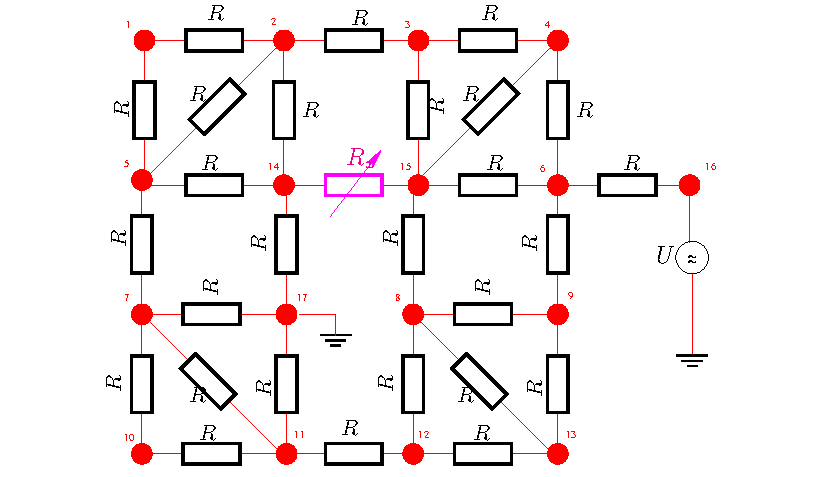
\includegraphics[width=0.9\textwidth]{\problems/\chpt/PICTURES/rcircuit_convert.pdf}
    \caption{Resistor circuit with a single controlled resistance}
    \label{fig:rcircuit}
  \end{figure}
  

\begin{subproblem}[2]\label{cimp:sp:1}
  Study \lref{ex:elnet} that explains how to compute voltages and currents in a
  linear circuit by means of nodal analysis. Understand how this leads to a linear
  system of equations for the unknown nodal potentials. The fundamental laws of
  circuit analysis should be known from physics as well as the principles of nodal
  analysis.
\end{subproblem}

\begin{subproblem}[3]\label{cimp:sp:2}
  Use nodal analysis to derive the linear system of equations satisfied by 
  the nodal potentials of the circuit from Figure~\ref{fig:rcircuit}. 
  The voltage $W$ is applied to node \#16 and node \#17 is grounded. 
  All resistors except for the controlled one (colored magenta) 
  have the same resistance $R$.
  Use the numbering of nodes indicated in Figure~\ref{fig:rcircuit}.
  
  \begin{hint}
    Optionally, you can make the computer work for you and find a fast way to build
    a matrix providing only the essential data. This is less tedious, less error
    prone and more flexible than specifying each entry individually. For this you
    can use auxiliary data structures.
  \end{hint}
  
  \begin{solution}
   We use the Kirchhoff's first law (as in \lref{ex:elnet}), stating that the sum the currents incident to a node is zero. Let $\vec{W} \in \IR^{17}$ be the vector of voltages. Set $f(R_x) := R / R_x$. We rescale each sum multiplying by $R$. Let us denote by $\Delta W_{i,j} := (W_i - W_j)$. The system  for each node $i = 1,\dots,15$ becomes: 
   \begin{align} \label{eq:syst_impedance}
   \begin{cases} 
    \Delta W_{1,2} + \Delta W_{1,5} & = 0 \\
    \Delta W_{2,1} + \Delta W_{2,3} + \Delta W_{2,5} + \Delta W_{2,14} & = 0 \\
    \Delta W_{3,2} + \Delta W_{3,4} + \Delta W_{3,15} & = 0 \\
    \Delta W_{4,3} + \Delta W_{4,6} + \Delta W_{4,15} & = 0 \\
    \Delta W_{5,1} + \Delta W_{5,2} + \Delta W_{5,7} + \Delta W_{5,14} & = 0 \\
    \Delta W_{6,4} + \Delta W_{6,9} + \Delta W_{6,15} + \Delta W_{6,16} & = 0 \\
    \Delta W_{7,5} + \Delta W_{7,10} + \Delta W_{7,11} + \Delta W_{7,17} & = 0 \\
    \Delta W_{8,9} + \Delta W_{8,12} + \Delta W_{8,13} + \Delta W_{8,5} & = 0 \\
    \Delta W_{9,6} + \Delta W_{9,8} + \Delta W_{9,13} & = 0 \\
    \Delta W_{10,7} + \Delta W_{10,11} & = 0 \\
    \Delta W_{11,7} + \Delta W_{11,10} + \Delta W_{11,12} + \Delta W_{11,17} & = 0 \\
    \Delta W_{12,8} + \Delta W_{12,11} + \Delta W_{12,13} & = 0 \\
    \Delta W_{13,8} + \Delta W_{13,9} + \Delta W_{13,12} & = 0 \\
    \Delta W_{14,2} + \Delta W_{14,5} + \Delta W_{14,17} + f(R_x) \Delta W_{14,15} & = 0 \\
    \Delta W_{15,3} + \Delta W_{15,4} + \Delta W_{15,6} + \Delta W_{15,8} + f(R_x) \Delta W_{15,14} & = 0
   \end{cases}
   \end{align}
   with the extra condition $W_{16} := W, W_{17} = 0$. We now have to obtain the system matrix. The system is rewritten in the following matrix notation (with $\vec{C} \in \IR^{15,17}$):
   \[
    \vec{C} = [\vec{A}(R_x), \vec{B}] \vec{W} = \vec{0} \; \Leftrightarrow \; \vec{A}(R_x) \tilde{\vec{W}} = - \vec{B} \cdot [W_{16}, \; W_{17}]^\top =: rhs
   \]
   with $\vec{W} = [\vec{\tilde{W}}, \; W_{16}, \; W_{17}]$, and with:
   \setcounter{MaxMatrixCols}{20}
   \begin{align*}
    \vec{A}(R_x) = \begin{bmatrix} 
      2 & -1 & 0 & 0 & -1 & 0 & 0 & 0 & 0 & 0 & 0 & 0 & 0 & 0 & 0 \\
      -1 & 4 & -1 & 0 & -1 & 0 & 0 & 0 & 0 & 0 & 0 & 0 & 0 & -1 & 0 \\
      0 & -1 & 3 & -1 & 0 & 0 & 0 & 0 & 0 & 0 & 0 & 0 & 0 & 0 & -1 \\
      0 & 0 & -1 & 3 & 0 & -1 & 0 & 0 & 0 & 0 & 0 & 0 & 0 & 0 & -1 \\
      -1 & -1 & 0 & 0 & 4 & 0 & -1 & 0 & 0 & 0 & 0 & 0 & 0 & -1 & 0 \\
      0 & 0 & 0 & -1 & 0 & 4 & 0 & 0 & -1 & 0 & 0 & 0 & 0 & 0 & -1 \\
      0 & 0 & 0 & 0 & -1 & 0 & 4 & 0 & 0 & -1 & -1 & 0 & 0 & 0 & 0 \\
      0 & 0 & 0 & 0 & 0 & 0 & 0 & 4 & -1 & 0 & 0 & -1 & -1 & 0 & -1 \\
      0 & 0 & 0 & 0 & 0 & -1 & 0 & -1 & 3 & 0 & 0 & 0 & -1 & 0 & 0 \\
      0 & 0 & 0 & 0 & 0 & 0 & -1 & 0 & 0 & 2 & -1 & 0 & 0 & 0 & 0 \\
      0 & 0 & 0 & 0 & 0 & 0 & -1 & 0 & 0 & -1 & 4 & -1 & 0 & 0 & 0 \\
      0 & 0 & 0 & 0 & 0 & 0 & 0 & -1 & 0 & 0 & -1 & 3 & -1 & 0 & 0 \\
      0 & 0 & 0 & 0 & 0 & 0 & 0 & -1 & -1 & 0 & 0 & -1 & 3 & 0 & 0 \\
      0 & -1 & 0 & 0 & -1 & 0 & 0 & 0 & 0 & 0 & 0 & 0 & 0 & 3 + \frac{R}{R_x} & -\frac{R}{R_x} \\
      0 & 0 & -1 & -1 & 0 & -1 & 0 & -1 & 0 & 0 & 0 & 0 & 0 & -\frac{R}{R_x} & 4 + \frac{R}{R_x} \\
        \end{bmatrix} \\
   \end{align*}
    a square $15 \times 15$ matrix and $\vec{B} \in \IR^{15,2}$ zero except $B_{6,1} = -R$.

   (For each term with the form $\beta \cdot \Delta W_{i,j}$ in \eqref{eq:syst_impedance} we have add an entry $\beta$ in the diagonal $i,i$ and an entry $-\beta$ in the cell $i,j$ (if $j \leq 15$). Entries with $j > 15$ will produce a corresponding positive entry $\beta \cdot U_j$ in the r.h.s.)
  \end{solution}

\end{subproblem}

\begin{subproblem}[3]\label{cimp:sp:3}
  Characterize the change in the circuit matrix derived in
  sub-problem~\ref{cimp:sp:2} induced by a change in the value of $R_{x}$ 
  as a low-rank modification of the circuit matrix. Use as a base state $R = R_x$.

  \begin{hint}
    Four entries of the circuit matrix will change. This amounts to
    a rank-2-modification in the sense of \lref{mod:1} with suitable
    matrices $\Vu$ and $\Vv$. 
  \end{hint}
  
  \begin{solution}
   The matrices
   \begin{align*}
    \vec{U} = \begin{bmatrix}
               0 & 0 \\
               \vdots & \vdots \\
               -1 & 1 \\
               1 & -1
              \end{bmatrix} = \vec{V}
   \end{align*}
   are such that $\vec{A}(R)$ defined as $\vec{A}(R_x)$ allows to write:
   \begin{align*}
    \vec{A}(R_x) = \vec{A}(R) - \vec{U} \vec{V^\top} \left(1 - \frac{R}{R_x} \right) / {2}.
   \end{align*}
   Therefore, if we already have the factorization of $\vec{A}_0$, we can use the SMW formula for the cheap inversion of $\vec{A}(R_x)$.
\end{solution}

\end{subproblem}

\begin{subproblem}[3]
  Based on the \eigen{} library, implement a C++ class 
\begin{lstlisting}[style=cppsimple]
class ImpedanceMap {
public:
  ImpedanceMap(double R_, double W_) : R(R_), W(W_) {
      // TODO: build A0 = A(1), the rhs and factorize A\_0 with lu = A0.lu()
  };
  double operator() (double Rx) const {
      // TODO: compute the perturbation matrix U and solve ($A + UU^T$) x = rhs, from x, U and R compute the impedance
  };
private:
  Eigen::PartialPivLU<Eigen::MatrixXd>> lu;
  Eigen::VectorXd rhs;
  double R, W;
};   
\end{lstlisting}
whose \texttt{()}-operator returns the impedance of the circuit from 
Figure~\ref{fig:rcircuit} when supplied with a concrete value for $R_{x}$.
Of course, this function should be implemented efficiently using 
\lref{lem:SMW}. The setup phase of Gaussian elimination should be carried
out in the constructor performing the LU-factorization of the circuit matrix.

Test your class using $R = 1, W = 1$ and $R_x=1,2,4,\cdots,1024$.
\begin{hint}
 See the file \texttt{impedancemap.cpp}.
\end{hint}

\begin{hint}
  The impedance of the circuit is the quotient of the voltage at the
  input node \#16 and the current through the voltage source.
\end{hint}

% \begin{hint}
%  Remember Ohm's law $I = \Delta V / R$.
% \end{hint}

\end{subproblem}


\end{problem}

\end{sheet}

%%% PS4
\begin{sheet}{4}{08.10.2015}{15.10.2015}
% ncse_new/p1_SystemsOfEquations/ch3_IterativeMethodsNonLinear/ex_RecursionOrder.tex
\renewcommand{\chpt}{ch_iterativenonlinear}

\begin{problem}[Order of convergence from error recursion \coreproblem] \label{prb:RecursionOrder}

In \lref{ex:sec} we have observed \emph{fractional} orders of convergence ($\to$
\ncsedef{def:cvgord}) for both the secant method, see \ncseref[Code]{mc:secant},
and the quadratic inverse interpolation method. This is fairly typical for 2-point
methods in 1D and arises from the underlying recursions for error bounds. The
analysis is elaborated for the secant method in \lref{rem:secfraccvg}, where a
linearized error recursion is given in \lref{eq:secanterrprop}.

Now we suppose the recursive bound for the norms of the iteration errors
\begin{gather}    
  \label{eq:prb:RecursionOrder}
\|e^{(n+1)}\|\leq \|e^{(n)}\| \sqrt{\|e^{(n-1)}\|}\;,
\end{gather}
where $e^{(n)}=x^{(n)}-x^{*}$ is the error of $n$-th iterate. 

\begin{subproblem}[1]\label{prb:RecursionOrder_1}
Guess the maximal order of convergence of the method from a numerical experiment
conducted in MATLAB. \\
\hint \ncserem{rem:eoc}

\begin{solution}
See Listing~\ref{mc:recursionorder}.
\lstinputlisting[caption={MATLAB script for Sub-problem
    ~\ref{prb:RecursionOrder_1}}, label={mc:recursionorder}]{\problems/ch_iterativenonlinear/MATLAB/recursionorder.m}
  \end{solution}
  \end{subproblem}

\begin{subproblem}[4]\label{prb:RecursionOrder_2}
Find the maximal
guaranteed order of convergence of this method through analytical considerations.

\begin{hint}
 First of all note that we may assume equality in both the error
recursion \eqref{eq:prb:RecursionOrder} and the bound $\|e^{(n+1)}\|\leq C\|e^{(n)}\|^{p}$ that
defines convergence of order $p>1$, because in both cases equality corresponds to a
worst case scenario. Then plug the two equations into each other and obtain
an equation of the type $\ldots = 1$, where the left hand side involves an 
error norm that can become arbitrarily small. This implies a condition on
$p$ and allows to determine $C>0$. A formal proof by induction (not required)
can finally establish that these values provide a correct choice. 
\end{hint}



\begin{solution}
Suppose $\|e^{(n)}\|=C \|e^{(n-1)}\|^{p}$ ($p$ is the largest convergence order and C is some constant).\\
Then
\begin{gather}
  \label{RO:1}
  \|e^{(n+1)}\|=C\|e^{(n)}\|^{p}
  =C(C\|e^{(n-1)}\|^p)^{p}
  =C^{p+1}\|e^{(n-1)}\|^{p^2}
\end{gather}
In \eqref{eq:prb:RecursionOrder} we may assume equality, because this is the worst case.
Thus,
\begin{gather}
  \label{RO:2}
\|e^{(n+1)}\| = \|e^{(n)}\|\cdot \|e^{(n-1)}\|^\frac{1}{2}
=C\|e^{(n-1)}\|^{p+\frac{1}{2}}
\end{gather}
Combine \eqref{RO:1} and \eqref{RO:2},
$$C^{p+1}\|e^{(n-1)}\|^{p^2} = C\|e^{(n-1)}\|^{p+\frac{1}{2}}$$
i.e.
 \begin{gather}
   \label{RO:3}
 C^{p}\|e^{(n-1)}\|^{p^2-p-\frac{1}{2}} = 1.
 \end{gather}
Since \eqref{RO:3} holds for each $n\geq 1$, we have \\
$$p^2-p-\frac{1}{2}=0$$
$$p=\frac{1+\sqrt{3}}{2} ~~~~~{\rm or}~~~~~~p=\frac{1-\sqrt{3}}{2}~
{\rm(dropped)}.$$
For $C$ we find the maximal value $1$.
 \end{solution}
  \end{subproblem}
  \end{problem}

\begin{problem}[Convergent Newton iteration \coreproblem] \label{prb:new_iter}
  As explained in \ncsesect{sec:newton-verfahren-1d}, the convergence of Newton's method in 1D may only be local. This problem
  investigates a particular setting, in which global convergence can be expected. 

  We recall the notion of a \emph{convex function} and its geometric definition.  A
  differentiable function $f:[a,b]\mapsto \bbR$ is convex, if and only if its graph
  lies on or above its tangent at any point. Equivalently, differentiable function
  $f:[a,b]\mapsto \bbR$ is convex, if and only if its derivative is non-decreasing. 

  Give a ``graphical proof'' of the following statement:

  If $F(x)$ belongs to $C^{2}(\mathbb{R})$, is strictly increasing, is convex, and
  has a unique zero, then the Newton iteration \ncseeq{eq:Newton1D} for $F(x)=0$ is
  well defined and will converge to the zero of $F(x)$ for any initial guess
  $x^{(0)}\in\bbR$.
  
\cprotEnv \begin{solution}
    The sketches in Figure~\ref{fig:graph_proof_newt} discuss the different cases.
\begin{figure}[h!]
\begin{centering}
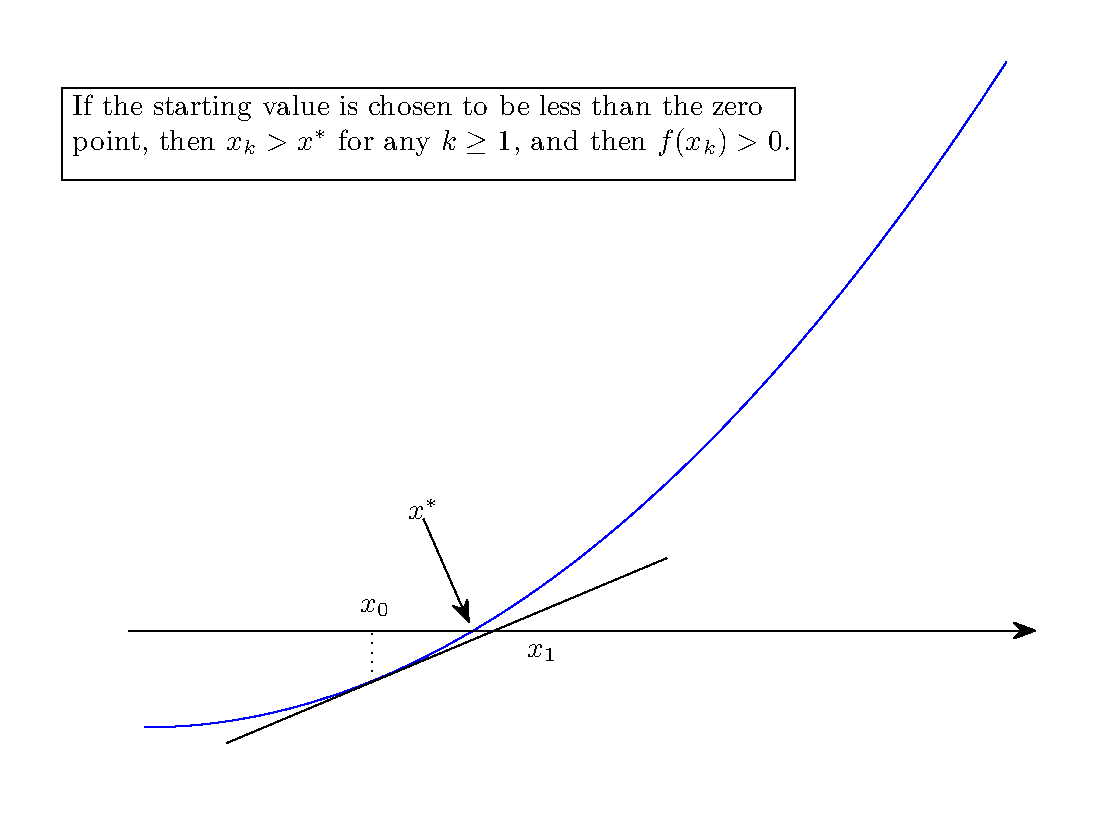
\includegraphics[width=0.7\textwidth]{\problems/\chpt/PICTURES/P2a.pdf}
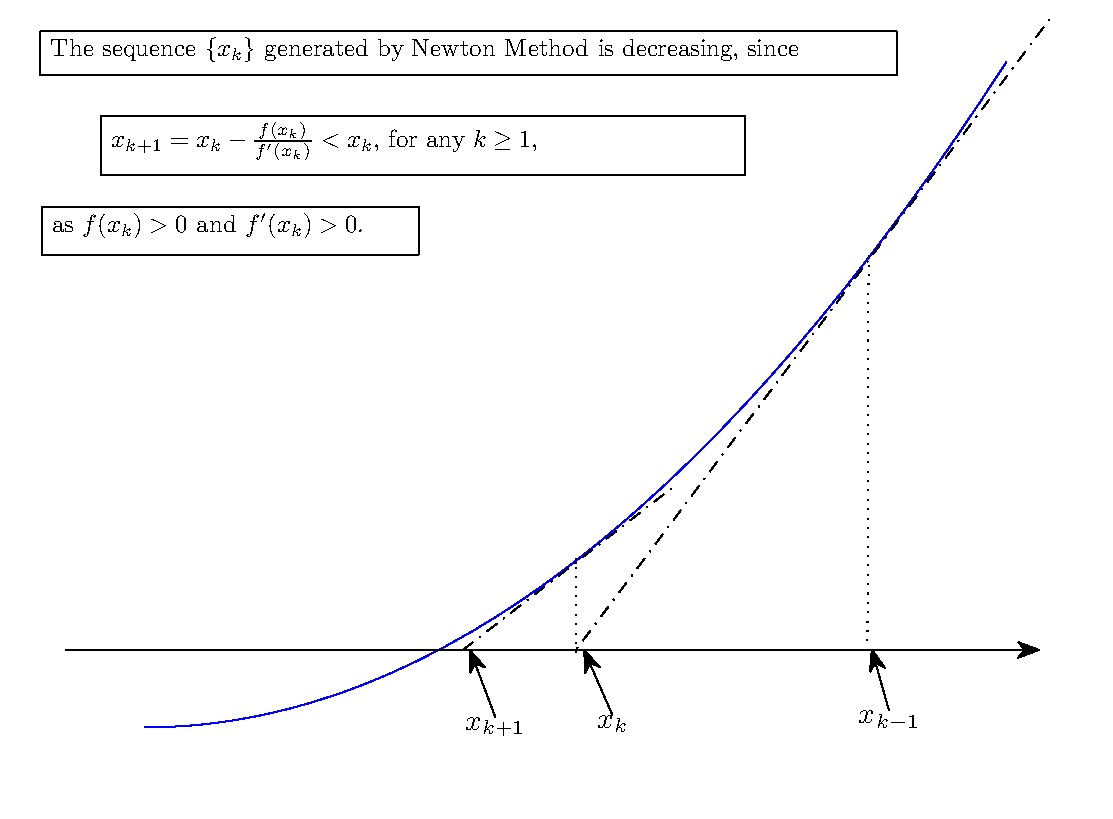
\includegraphics[width=0.7\textwidth]{\problems/\chpt/PICTURES/p2b.pdf}
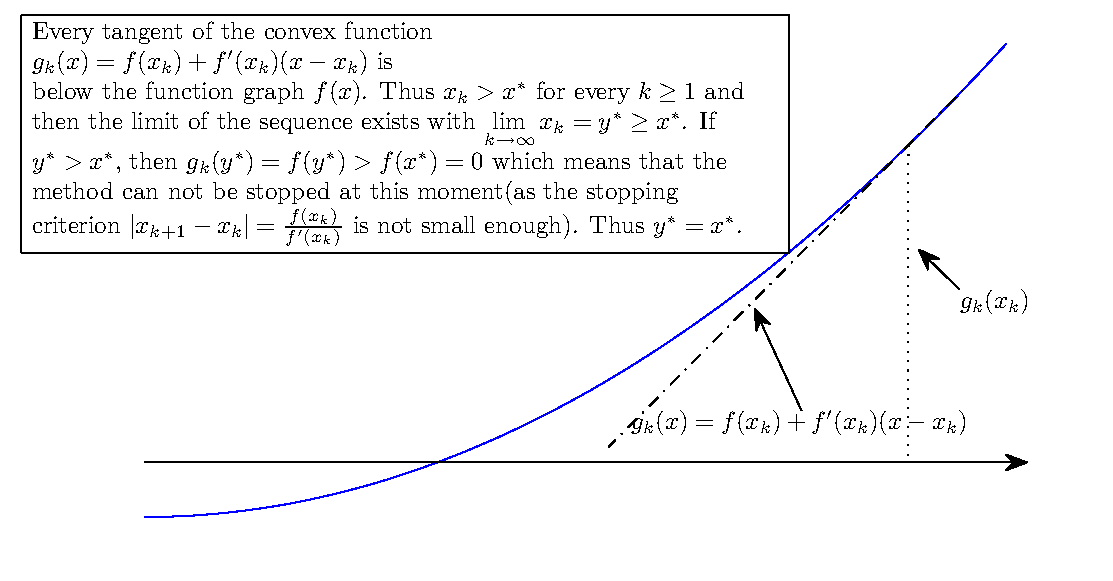
\includegraphics[width=0.7\textwidth]{\problems/\chpt/PICTURES/p2c.pdf}
\caption{Graphical proof for \ref{prb:new_iter}}
\label{fig:graph_proof_newt}
\end{centering}
\end{figure}
\end{solution}

\end{problem}
% ncse_new/p1_SystemsOfEquations/ch3_IterativeMethodsNonLinear/ex_QuadraticConvergence.tex
% ex_OrderConv.m


\begin{problem}[The order of convergence of an iterative scheme \coreproblem] \label{prb:QuadraticConvergence}
%  \ncseref[Lemma]{lem:fpcvg} gives a criterion for higher order local convergence of a fixed point iteration $x=\Phi(x)$ in 1D.

\lref{rem:eoc} shows how to detect the order of convergence of an iterative method
from a numerical experiment. In this problem we study the so-called
\href{http://en.wikipedia.org/wiki/Steffensen's_method}{Steffensen's method},
which is a derivative-free iterative method for finding zeros of functions in 1D.

Let $f:[a,b]\mapsto\bbR$ be twice continuously differentiable with $f(x^{\ast})=0$ and $f'(x^{\ast})\not=0$.
Consider the iteration defined by
$$ x^{(n+1)}=x^{(n)}-\frac{f(x^{(n)})}{g(x^{(n)})},\quad \text{where}\quad g(x)=\frac{f(x+f(x))-f(x)}{f(x)}.$$

\begin{subproblem}[2]
Write a \Matlab{} script that computes the order of convergence to the point $x^*$ of this iteration for the function $f(x)=xe^x-1$ (see \ncseex{ex:fixp}). Use $x^{(0)} = 1$.

\cprotEnv \begin{solution}
\lstinputlisting[caption={Order of convergence}, label={mc:ex_OrderConv}, escapechar={}]
{\problems/\chpt/MATLAB/ex_OrderConv.m}

The output is\\
\begin{center}
\begin{tabular}{lll}
   $x$   &          error $e_n$   &   $\frac{\log(e_{n+1})-\log(e_n)}{\log(e_{n})-\log(e_n-1)}$ \\
   \hline
   $1.000000000000000 $ & $  0.432856709590216  $ &                    \\
   $0.923262600967822 $ & $  0.356119310558038  $ &                   \\
   $0.830705934728425 $ & $  0.263562644318641  $ & $    1.542345498206531$\\
   $0.727518499997190 $ & $  0.160375209587406  $ & $    1.650553641703975$\\
   $0.633710518522047 $ & $  0.066567228112263  $ & $    1.770024323911885$\\
   $0.579846053882820 $ & $  0.012702763473036  $ & $    1.883754995643305$\\
   $0.567633791946526 $ & $  0.000490501536742  $ & $    {\red1.964598248590593}$\\
   $0.567144031581974 $ & $  0.000000741172191  $ & $    {\red1.995899954235929}$\\
   $0.567143290411477 $ & $  0.000000000001693  $ & $    {\red1.999927865685712}$\\
   $0.567143290409784 $ & $  0.000000000000000  $ & $    0.741551601040667$
\end{tabular}
\end{center}

The convergence is obviously quadratic. As in the experiments shown in class,
roundoff affects the estimated order, once the iteration error approaches the
machine precision. 
\end{solution}
\end{subproblem}

\begin{subproblem}[2]
The function $g(x)$ contains a term like $e^{xe^x}$, thus it grows very fast in $x$ and the method can not be started for a large $x^{(0)}$.
How can you modify the function $f$ (keeping the same zero) in order to allow the choice of a larger initial guess?

\begin{hint}
 If $f$ is a function and $h: [a,b] \rightarrow \IR$ with $h(x) \neq 0, \forall x \in [a,b]$, then $(fh)(x) = 0 \Leftrightarrow f(x) = 0$.
\end{hint}


\cprotEnv \begin{solution}
The choice $\tilde f(x) = e^{-x}f(x)= x-e^{-x}$ prevents the blow up of the function $g$ and allows to use a larger set of positive initial points.
Of course, $\tilde f(x)=0$ exactly when $f(x)=0$.

\end{solution}
\end{subproblem}
\end{problem}

% 2009:  proof of 2nd order with Taylor, messy
%
%   Show that this iteration is locally quadratically convergent to $x^{\ast}$.
%
% \verbdef\QuadConvVa{f    := x -> (x-xs)*h(x);}
% \verbdef\QuadConvVb{g    := x -> ( f(x+f(x))-f(x) ) / f(x);}
% \verbdef\QuadConvVc{Phi  := x -> x-f(x)/g(x);}
% \verbdef\QuadConvVd{dPhi := D(Phi)(x);}
% \verbdef\QuadConvVe{limit(%,x=xs);}
% \solution{
% This exercise can be treated in two different ways. Either one uses the indicated lemma or one accomplishes a Taylor expansion to estimate the error expansion.
% Both ways are rather write intensive.
% Therefore the first approach is worked out using the formula manipulation program MAPLE:
% \begin{enumerate}
% \item   We define the function $$\Phi(x)=x -\frac{f(x)}{g(x)} $$
% To show that the fixed point iteration converges quadratically it must hold: $\frac{\partial \Phi(x)}{\partial x}\big\vert_{x=x^*}=0$.
% In MAPLE we write:\\
% \QuadConvVa\\
% \QuadConvVb\\
% \QuadConvVc\\
% \QuadConvVd\\
% \QuadConvVe\\
% The result is essentially $0$. Thus the given method converges quadratically.
% \bigskip
%
% \item
%   $e^{(n)}=x^{(n)}-x^{*}$ is the error of $n^{th}$ iteration by the iteration formula.
%   Supposing $f(x)$ is smooth enough we can use Taylor expansion to express $f(x)$ and
%   $f(x+f(x))$ at $x^{(*)}$ respectively (notice that $f(x^{(*)})=0$):
%   \begin{eqnarray*}
%   f(x^{(n)})&=&f'(x^{(*)})e^{(n)}+f''(x^{*})(e^{(n)})^{2}+O((e^{(n)})^3)\\
%   f(x^{(n)}+f(x^{(n)}))&=&f'(x^{(*)})(1+f'(x^{(*)}))e^{(n)}\\
%   &&+[f''(x^{*})(1+f'(x^{*}))^2+f'(x^{*})f''(x^{*})](e^{(n)})^{2}+O((e^{(n)})^3)
%   \end{eqnarray*}
%   Then
%   \begin{eqnarray*}
%   e^{(n+1)}&=&x^{(n+1)}-x^{*}\\
%   &=&x^{(n)}-x^{*}-\frac{f(x^{(n)})}{g(x^{(n)})}\\
%   &=&e^{(n)}-\frac{f(x^{(n)})}{g(x^{(n)})}\\
% &=&\frac{[f(x^{(n)}+f(x^{(n)}))-f(x^{(n)})]e^{(n)}-f^2(x^{(n)})}{f(x^{(n)}+f(x^{(n)}))-f(x^{(n)})}\\
% &=&\frac{[(f'(x^{*})^{2}f''(x^{*})+f'(x^{*})f''(x^{*})](e^{(n)})^3+O((e^{(n)})^4)}
% {(f'(x^{*}))^2e^{(n)}+O((e^{(n)})^2)}\\
% &\approx & C(e^{(n)})^{2}
%  \end{eqnarray*}
% where $ C=\frac{f''(x^{*})+f'(x^{*})f''(x^{*})}{f'(x^{*})}$.
% So if $f(x)$ belongs to $C^{2}(\mathbb{R})$ and $x^{*}$ is a simple zero of $f(x)$, then the iteration is locally quadratically convergent.
% \end{enumerate}
% }
%

% ncse_new/p1_SystemsOfEquations/ch3_IterativeMethodsNonLinear/ex_NewtonArctan.tex
% solution:    NewtonArctan.m    ex_NewtonArctan.eps



\begin{problem}[Newton's method for \texorpdfstring{$F(x):=\arctan x$}{\emph{F(x):=arctan x} \coreproblem}]\label{prb:NewtonArctan}

  The merely local convergence of Newton's method is notorious, see\lref{sec:konv-des-newt}  and \lref{ex:loccvgnewt}.
  The failure of the convergence is often caused by the overshooting of Newton correction.
  In this problem we try to understand the observations made in \lref{ex:loccvgnewt}.

\begin{subproblem}[4]
  Find an equation satisfied by the smallest positive initial guess $x^{(0)}$ for which Newton's method does not converge when it is applied to  $F(x)=\arctan{x}$.
  \begin{hint}
  Find out when the Newton method oscillates between two values.
  \end{hint}
    \begin{hint}
  Graphical considerations may help you to find the solutions. See Figure~\ref{fig:newtonarctan}: you should find an expression for the function $g$.
  \begin{figure}
\caption{Newton iterations with $F(x)=\arctan(x)$ for the critical initial value $x^{(0)}$}
\begin{center} 
\label{fig:newtonarctan}
\includegraphics[width=0.6\textwidth]{\problems/ch_iterativenonlinear/PICTURES/ex_NewtonArctan.eps}
\end{center}
\end{figure}
  \end{hint}

% \Matlab's \texttt{fzero} function to compute it.  Rely on geometric considerations.


\begin{solution}The function $\arctan(x)$ is \textbf{positive, increasing and concave} for positive $x$, therefore the first iterations of Newton's method with initial points $0<x^{(0)}<y^{(0)}$ satisfy $ y^{(1)}<x^{(1)}<0$ (draw a sketch to see it).
The function is \textbf{odd}, i.e., $\arctan(-x)=-\arctan(x)$ for every $x\in\IR$, therefore the analogous holds for initial negative values ($y^{(0)}<x^{(0)}<0$ gives $0<x^{(1)}<y^{(1)}$).
Moreover, opposite initial values give opposite iterations: if $y^{(0)}=-x^{(0)}$ then $y^{(n)}=-x^{(n)}$ for every $n\in\IN$.

All these facts imply that, if $|x^{(1)}|<|x^{(0)}|$, then the absolute values of the following iterations will converge monotonically to zero.
Vice versa, if $|x^{(1)}|>|x^{(0)}|$, then  the absolute values of the Newton's iterations will diverge monotonically.
Moreover, the iterations change sign at each step, i.e., $x^{(n)}\cdot x^{(n+1)}<0$.

%Newton's method diverges for $f(x)=\arctan{x}$ if and only if $|x^{(n+1)}|\geq |x^{(n)}|$, so
It follows that the smallest positive initial guess $x^{(0)}$ for which Newton's method does not converge satisfies  $x^{(1)}= -x^{(0)}$.
This can be written as
$$x^{(1)}=x^{(0)}-\frac{f(x^{(0)})}{f'(x^{(0)})}=x^{(0)}-(1+(x^{(0)})^2)\arctan{x^{(0)}}= - x^{(0)}.$$
%The function $\arctan(x)$ is convex and negative for $x<0$ and concave and positive for $x>0$; therefore at each Newton iteration the points $x^(n)$ and $x^{(n+1)}$ have opposite signs (you can check this fact with a simple drawing).
%Thus, in the formula above we have to choose the negative sign, i.e., $x^{(1)}=-x^{(0)}$.
   Therefore, $x^{(0)}$ is  a zero of the function
    $$g(x)=2x-(1+x^2)\arctan{x} \quad \text{with} \quad g'(x)=1-2x\arctan{x}.$$
   \end{solution}
\end{subproblem}

\begin{subproblem}[2]
Use Newton's method to find an approximation of such $x^{(0)}$, and implement it with Matlab.
\cprotEnv\begin{solution}
    Newton's iteration to find the smallest positive initial guess reads
    $$x^{(n+1)}=x^{(n)}-\frac{2x^{(n)}-(1+(x^{(n)})^2)\arctan{x^{(n)}}}{1-2x\arctan{x^{(n)}}}
= \frac{ -x^{(n)}+\big(1-(x^{(n)})^2\big)\arctan x^{(n)} }{1-2x^{(n)}\arctan x^{(n)}}.$$

The implementation in Matlab is given in Listing~\ref{mc:NewtonArctan} (see also Figure~\ref{fig:newtonarctan}).

\lstinputlisting[caption={Matlab Code for \texttt{NewtonArctan.m}}, label={mc:NewtonArctan}]{\problems/ch_iterativenonlinear/MATLAB/NewtonArctan.m}





\end{solution}
\end{subproblem}

\end{problem}



% NO, WRONG:
% \textbf{Remark}: this is an example on a general phenomenon.
% Given an iterative procedure $x^{(n+1)}=\Phi(x^{(n)})$, we call a \textit{cycle} of order $k>1$ a point $x^{(0)}$ such that $x^{(k)}=x^{(0)}$ and $x^{(1)},x^{(2)},\ldots x^{(k-1)}\neq x^{(0)}$.
% A cycle of order $k$ is computed as the zero of the iterated function $g(x)=\Phi^k(x)=\Phi\circ\ldots\circ\Phi(x)$.
%
% In our case $\Phi(x)=x-F(x)/F'(x)$ is the Newton's iteration, $k=2$ and $g(x)=\Phi(\Phi(x))$.





% \subproblem\label{subprb:NewtonArctan_1}
% Consider a function $F:\IR\rightarrow \IR$ such that
% \begin{itemize}
% \item $F$ is of class $C^1(\IR)$;
% \item $F$ is odd: $F(-x) = F(x)$, $\forall\;x\in\IR$;
% \item the derivative satisfies $0<F'(x)\le 1$, $\forall\;x\in\IR$.
% \end{itemize}
% Since $F$ is strictly monotonic and odd, it follows easily that $F(x)=0$ if and only if $x=0$.
% We denote $\{x^{(k)}\}_{k=1,2,\ldots}$ a sequence of Newton iterations, i.e., $x^{(k+1)} = x^{(k)}-F(x^{(k)})/F'(x^{(k)})$, for every $k=1,2,\ldots$
%
% Prove that, for every $k\ge1$,
%  $$ \text{if}\quad0<|x^{(k+1)}|<|x^{(k)}|\quad \text{then} \quad|x^{(k+2)}|<|x^{(k+1)}|,$$
% i.e., if at the step $k$ the method is approaching the unique zero of $F$, then it will approach the zero also in the following step.
%
% \solution{We have
% \begin{align*}
%  \frac{|x^{(k+2)}|}{|x^{(k+1)}|}&
% =\frac{|x^{(k+1)}-F(x^{(k+1)})/F'(x^{(k+1)})|}{|x^{(k+1)}|}
% =\frac{|x^{(k+1)}| \cdot |1-\frac{F(x^{(k+1)})}{x^{(k+1)}}  \frac1{F'(x^{(k+1)})} | }{|x^{(k+1)}|}\\
% &= \Big|1-\underbrace{\frac{F(x^{(k+1)})}{x^{(k+1)}}}_{\in(0,1]}  \underbrace{\frac1{F'(x^{(k+1)})}}_{\in(0,1],\;\text{by }ii)} \Big|<1;
% \end{align*}
% the ratio $\frac{F(x^{(k+1)})}{x^{(k+1)}}$ is positive because an odd increasing function always has the same sign of its argument, it is smaller or equal 1 because the derivative is not larger than 1 and $F(0)=0$.
% }
%

\renewcommand{\chpt}{ch_iterativenonlinear} 

\begin{problem}[Order-$p$ convergent iterations] \label{prb:ord_p_conv_iter}
  In \ncsesect{sec:speed-convergence} we investigated the speed of convergence of
  iterative methods for the solution of a general non-linear problem $F(\Vx) = 0$
  and introduced the notion of convergence of order $p \geq 1$, see \ncsedef{def:cvgord}.
  This problem highlights the fact that for $p>1$ convergence may not be guaranteed,
  even if the error norm estimate of \ncsedef{def:cvgord} may hold for some
  $\Vx^{\ast}\in \bbR^{n}$ and all iterates $\Vx^{(k)}\in\bbR^{n}$. 

  Suppose that, given $\Vx^{\ast}\in\bbR^{n}$, a sequence $\Vx^{(k)}$ satisfies
  $$\Vert \Vx^{(k+1)}-\Vx^*\Vert\;\le\; C\Vert \Vx^{(k)}-\Vx^*\Vert^p \qquad \forall k\quad
  \text{and some}\quad p>1\;. $$
  \begin{subproblem}[3]
    Determine $\epsilon_0>0$ such that 
    $$\Vert \Vx^{(0)}-\Vx^*\Vert \le \epsilon_0 \qquad \Longrightarrow \qquad
    \lim\limits_{k\rightarrow \infty} \Vx^{(k)}=\Vx^*.$$
    In other words, $\epsilon_{0}$ tells us which distance of the initial guess from 
    $\Vx^{\ast}$ still guarantees local convergence. 
    
    
    \begin{solution}
    $$\quad\lim\limits_{k\rightarrow\infty} x^{(k)}=x^* \iff \lim\limits_{k\rightarrow\infty}\Vert x^{(k)}-x^*\Vert=0$$
    Thus we seek an upper bound $B(k)$ for $\Vert x^{(k)}-x^*\Vert$ and claim that: $\lim\limits_{k\rightarrow\infty} B(k)=0$.  
        \begin{eqnarray}\Vert x^{(k)}-x^*\Vert &\le& C \Vert x^{(k-1)}-x^*\Vert^p \notag\\
                                                   &\le& C\cdot C^p \Vert x^{(k-2)}-x^* \Vert^{p^2} \notag \\
                                                   &\le& C\cdot C^p\cdot C^{p^2} \Vert x^{(k-3)}-x^*\Vert^{p^3} \notag \\
                                                   &\vdots& \notag \\
                                                   &\le& C\cdots C^{p^{k-1}}\Vert x^{(0)}-x^*\Vert^{p^k}\notag \\ 
                                                   &=& C^{\sum\limits_{i=0}^{k-1} p^i}\Vert x^{(0)}-x^*\Vert^{p^k}\notag \\
                                                   &\stackrel{\text{geom. series}}{=}& C^{\frac{p^k -1}{p-1}}\Vert x^{(0)}-x^*\Vert^{p^k}\notag \\
                                                   &\le& C^{\frac{p^k -1}{p-1}} \epsilon_0^{p^k} = \underbrace{C^{\frac{1}{1-p}}}_{\text{const.}}
                                                     \cdot\Big(C^{\frac{1}{p-1}}\epsilon_0\Big)^{p^k} = B(k) \notag
        \end{eqnarray}
     $$\lim\limits_{k\rightarrow\infty}B(k)=0 \qquad \iff \qquad  C^{\frac{1}{p-1}}\epsilon_0< 1$$
    $$\Longrightarrow \quad 0<\epsilon_0 < C^{\frac{1}{1-p}} $$
  \end{solution}
    \end{subproblem}
    \begin{subproblem}[2]
      Provided that $\Vert \Vx^{(0)}-\Vx^*\Vert < \epsilon_0$ is satisfied, determine
      the minimal $k_{\min}=k_{\min}(\epsilon_0,C,p,\tau)$ such that
    $$\Vert \Vx^{(k)}-\Vx^*\Vert < \tau.$$
    
    \begin{solution}
      Using the previous upper bound and the condition $\tau$, we obtain: 
      $$ \Vert x^{(k)}-x^*\Vert \le C^{\frac{1}{1-p}}\cdot\Big(C^{\frac{1}{p-1}}\epsilon_0\Big)^{p^k}<\tau$$
      Solving for the minimal $k$ (and calling the solution $k_{min}$), with the additional requirement that $k \in \IN$, we obtain:
      \begin{align*}
      \ln{\big(C^{\frac{1}{1-p}}\big)} + p^k\cdot\underbrace{\ln{\big(C^{\frac{1}{p-1}}\epsilon_0}\big)}_
                                         {<0} < \ln{\tau} \notag \\
      k>\ln{\Bigg(\frac{ \ln{\big(\tau)}+\frac{1}{p-1}\ln{(C)}}{\ln{(C^{\frac{1}{p-1}}\epsilon_0)}}}\Bigg)\cdot\frac{1}{\ln{(p)}},\qquad k_{min} \in \IN \\
      k_{min} = \Bigg\lceil\ln{\Bigg(\frac{ \ln{\big(\tau)}+\frac{1}{p-1}\ln{(C)}}{\ln{(C^{\frac{1}{p-1}}\epsilon_0)}}}\Bigg)\cdot\frac{1}{\ln{(p)}}\Bigg\rceil  \notag
      \end{align*}
    \end{solution}

    \end{subproblem}
    
    \begin{subproblem}[1]
    Write a \matlab{} function 
    
    \begin{verbatim}
      k_min = @(epsilon,C,p,tau) ...
    \end{verbatim} and plot 
    $k_{\min}=k_{\min}(\epsilon_0,\tau)$ for the values $p=1.5, C=2$. Test you implementation for every $(\epsilon_0, \tau)  \in \mathtt{linspace}(0,C^{\frac{1}{1-p}})^2 \cap (0,1)^2 \cap \{(i,j) \; | \; i \geq j  \}$
    
    \begin{hint}
     Use a \Matlab{} \verb|pcolor| plot and the commands \verb|linspace| and  \verb|meshgrid|.
    \end{hint}

    
   \cprotEnv \begin{solution}
   See \verb|k_min_plot.m|.
   
\lstinputlisting[caption={Matlab Code for \texttt{k\_min\_plot.m}, \ref{prb:ord_p_conv_iter}}, label={mc:k_min_plot},language=matlab, escapechar={}]{\problems/\chpt/MATLAB/k_min_plot.m}

\begin{figure}
    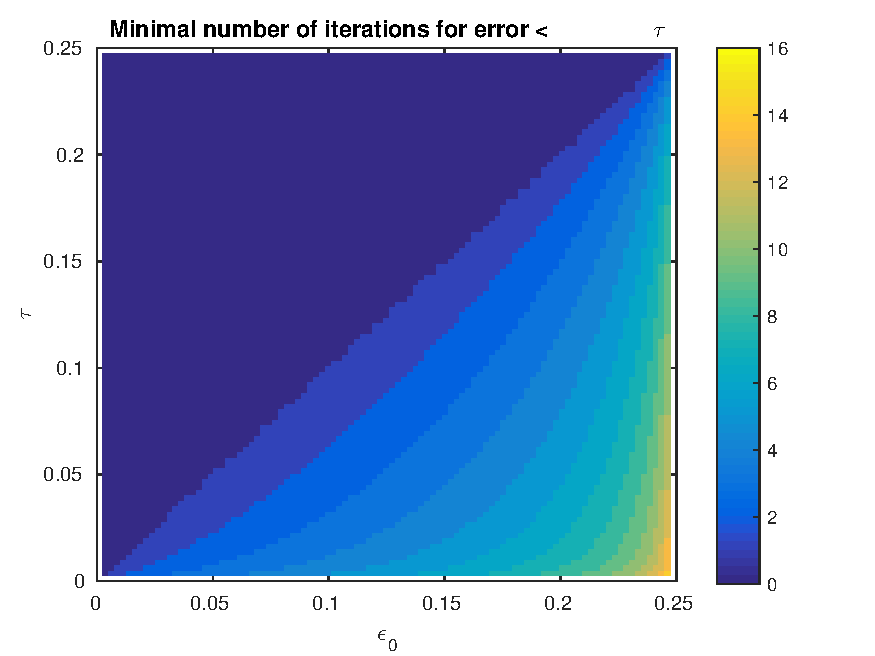
\includegraphics[scale=0.8]{\problems/\chpt/PICTURES/k_min.pdf}
\caption{Minimum number of iterations given $\tau$ and $\epsilon_0$, \ref{prb:ord_p_conv_iter}}
\end{figure}
    \end{solution}

    \end{subproblem}
\end{problem}

\begin{problem}[Code quiz]
  A frequently encountered drudgery in scientific computing is
  the use and modification of poorly documented code. This makes
  it necessary to understand the ideas behind the code first. 
  Now we practice this in the case of a simple iterative method. 

  \begin{subproblem}[4]
    What is the purpose of the following MATLAB code?
    \begin{lstlisting}[style=mcode]
     function y = myfn(x)
     log2 = 0.693147180559945;
     
     y = 0;
     while (x >   sqrt(2)), x = x/2; y = y + log2; end
     while (x < 1/sqrt(2)), x = x*2; y = y - log2; end
     z = x-1;
     dz = x*exp(-z)-1;
     while (abs(dz/z) > eps)
         z = z+dz;
        dz = x*exp(-z)-1;
     end
     y = y+z+dz;
\end{lstlisting}
\end{subproblem}
\begin{solution}
 The MATLAB code computes $y=\log{(x)}$, for a given $x$.
    The program can be regarded as Newton iterations for finding the zero of
    \begin{equation}\label{eq:func} f(z)=e^{z}-x\end{equation}
    where $z$ is unknown and $x$ is given.
\end{solution}

\begin{subproblem}[3]
  Explain the rationale behind the two \texttt{while} loops in
  lines \#5, 6.
  \begin{solution}
 The purpose of the two while loops is to shift the function values of (\ref{eq:func}) and
        modify the initial $z_0=x-1$ in such a way that good convergence is reached (according to the function derivative).
\end{solution}
\end{subproblem}
\begin{subproblem}[2]
  Explain the loop body of lines \#10, 11.
  \begin{solution}
The \texttt{while}-loop computes the zero of (\ref{eq:func}) using Newton iterations
  $$\left\{\begin{array}{lcc}z^{(0)}=x-1, \\
      z^{(n+1)}= z^{(n)}-\frac{e^{z^{(n)}}-x}{e^{z^{(n)}}},~~n\geq 1   \end{array}\right.
  $$
\end{solution}
\end{subproblem}
\begin{subproblem}[2]
  Explain the conditional expression in line \#9. 
  \begin{solution}
This is a correction based termination criterium, see \lref{par:tcpract}.
\end{solution}
\end{subproblem}
\begin{subproblem}[4]
  Replace the \texttt{while}-loop of lines \#9 through \#12 with a fixed number of iterations that,
  nevertheless, guarantee that the result has a relative accuracy $\mathtt{eps}$.
  
   \cprotEnv \begin{solution}
Denote the zero of $f(z)$ with $z^*$, and $e^{(n)}=z^{(n)}-z^*$.
Use Taylor expansion of $f(z),~f'(z)$:
\begin{eqnarray*}
f(z^{(n)})&=&e^{z^*}e^{(n)}+\frac{1}{2}e^{z^*}(e^{(n)})^2+O((e^{(n)})^3)\\
&=&xe^{(n)}+\frac{1}{2}x(e^{(n)})^2+O((e^{(n)})^3),\\
f'(z^{(n)})&=&e^{z^*}+e^{z^*}e^{(n)}+O((e^{(n)})^2)\\
&=&x+xe^{(n)}+O((e^{(n)})^2)
\end{eqnarray*}
Considering Newton's Iteration
$z^{(n+1)}=z^{(n)}-\frac{f(z^{(n)})}{f'(z^{(n)})}$,
\begin{eqnarray*}
e^{(n+1)}&=&e^{(n)}-\frac{f(z^{(n)}}{f'(z^{(n)}}\\
&=&e^{(n)}-\frac{xe^{(n)}+\frac{1}{2}x(e^{(n)})^2+O((e^{(n)})^3)}{x+xe^{(n)}+O((e^{(n)})^2)}\\
&\doteq&\frac{1}{2}(e^{(n)})^2\\
&=&\cdots\\
&\doteq&(\frac{1}{2})^{1+2+\cdots+2^n}(e^0)^{2^{n+1}}\\
&=&2\cdot(\frac{1}{2})^{2^{n+1}}(e^0)^{2^{n+1}}\\
&=&2\cdot(\frac{1}{2}e^0)^{2^{n+1}},
\end{eqnarray*}
where $e^0=z^0-z^*=x-1-\log{(x)}$. So it is enough for us to
 determine the number $n$ of iteration steps by
$|\frac{e^{(n+1)}}{\log{x}}|=\mathtt{eps}$. Thus
\begin{eqnarray*}
n&=&\frac{\log{(\log{(2)}-\log{(\log{(x)})}-\log{\mathtt{(eps)})}}-\log{(\log{(2)}-\log{(|e^0|)})}}{\log{(2)}}-1\\
&\approx & \frac{\log{(-\log{\mathtt{(eps)})}}-\log{(-\log{(|e^0|)})}}{\log{(2)}}-1
\end{eqnarray*}
The following code is for your reference.
\begin{lstlisting}[style=cppsimple]
 function y = myfn(x)
     log2 = 0.693147180559945;
     y = 0;
     while (x > sqrt(2)), x = x/2;  y = y + log2; end
     while (x < 1/sqrt(2)), x = x*2; y = y - log2; end
     z = x-1;
     dz = x*exp(-z)-1;
     e0=z-log(x);
     k=(log(-log(eps))-log(-log(abs(e0))))/log(2);
     for i=1:k
         z = z+dz;
         dz = x*exp(-z)-1;
     end
     y = y+z+dz;
\end{lstlisting}
\end{solution}
\end{subproblem}
\end{problem}
\end{sheet}

%%% PS5
\begin{sheet}{5}{15.10.2015}{22.10.2015}
% ncse_new/p1_SystemsOfEquations/ch3_IterativeMethodsNonLinear/ex_ModifiedNewton.tex
% the exercise requires:   -
% the solutions require:   ModNewtOrder.m  ModNewtStep.m  ModNewtSys.m  ModNewtOrder.eps
\renewcommand{\chpt}{ch_iterativenlse}

\begin{problem}[Modified Newton method \coreproblem] \label{prb:ModifiedNewton}

The following problem consists in \Eigen{} implementation of a modified version of the Newton method (in one dimension \ncsesect{sec:newton-verfahren-1d} and many dimensions \ncsesect{sec:Newton}) for the solution of a nonlinear system. Refresh yourself on stopping criteria for iterative methods \ncsesect{sec:termination-criteria-1}.

For the solution of the non-linear system of equations $\VF(\Vx) = \Vzero$ (with $\VF:\IR^n\rightarrow\IR^n$), the following iterative method can be used:
\begin{equation}  \label{eq:ABB10}
\begin{aligned}
\Vy^{(k)}   & = \Vx^{(k)} + D\VF(\Vx^{(k)})^{-1}\;\VF(\Vx^{(k)})\;,\\
\Vx^{(k+1)} & = \Vy^{(k)} - D\VF(\Vx^{(k)})^{-1}\;\VF(\Vy^{(k)})\;,
\end{aligned}
\end{equation}
where $D\VF(\Vx)\in\bbR^{n,n}$ is the Jacobian matrix of $\VF$ evaluated in the point $\Vx$.

%%%%%%%%%%%% SUBPROBLEM 1
\begin{subproblem}[2] \label{subprb:ModifiedNewton_1} Show that the iteration
  \eqref{eq:ABB10} is consistent with {$\VF(\Vx)=\Vzero$} in the sense of
  \lref{def:consitfp}, that is, show that $\Vx^{(k)} = \Vx^{(0)}$ for every $k\in\IN$, if and only if
  $\VF(\Vx^{(0)}) = \Vzero$ and $D\VF(\Vx^{(0)})$ is regular.

%%% 12.7 old version, prove consistency with IFF:
% Show that \eqref{eq:ABB10} provides a fixed point iteration that is consistent with $\VF(\Vx)=\Vzero$, provided that $D\VF$ is regular everywhere and $\VF$ is injective (i.e., $\VF(\Vx)=\VF(\Vy)\Leftrightarrow\Vx=\Vy$).
% 
% \hint: refer to Def.~4.2.1 from the course notes and use a slight generalization of it.
% 
% \andrea{added annoying hypothesis to match with slides def., they are supposed to show iff, more complicated }

\begin{solution}
If $\VF(\Vx^{(k)})=\Vzero$ then $\Vy^{(k)}=\Vx^{(k)}+\Vzero=\Vx^{(k)}$ and $\Vx^{(k+1)}=\Vy^{(k)}-\Vzero=\Vx^{(k)}$.\\
So, by induction, if $\VF(\Vx^{(0)})=\Vzero$ then $\Vx^{(k+1)}=\Vx^{(k)}=\Vx^{(0)}$ for every $k$.

Conversely, if $\vec{x}^{(k+1)} = \vec{x}^{(k)}$, then, by the recursion of the Newton method:
\begin{align*}
 \vec{F}(x^{(k)}) = \vec{F}(x^{(k)} + D\VF(\Vx^{(k)})^{-1}\;\VF(\Vx^{(k)})) \\
 \Rightarrow D\VF(\Vx^{(k)})^{-1}\;\VF(\Vx^{(k)}) = 0 \\
 \Rightarrow \VF(\Vx^{(k)}) = 0
\end{align*}
\end{solution}
\end{subproblem}

%%%%%%%%%%%% SUBPROBLEM 2
\begin{subproblem}[3] \label{subprb:ModifiedNewton_2}
Implement a \Cpp{} function
\begin{lstlisting}        
template <typename arg, class func, class jac>
void mod_newt_step(const arg & x, arg & x_next,
		   func&& f, jac&& df);
\end{lstlisting}
that computes a step of the method \eqref{eq:ABB10} for a \emph{scalar} function $\VF$, that is, for the case $n=1$. 

Here, \texttt{f} is a lambda function for the function $F:\bbR\mapsto\bbR$ and \texttt{df} a lambda to its derivative $F':\bbR\mapsto\bbR$.
\begin{hint}
Your lambda functions will likely be:
\begin{lstlisting}
auto f = [ /* captured vars. */ ] (double x)
	 { /* fun. body */ }; 
auto df = [ /* captured vars. */ ] (double x)
	  { /* fun. body */ }; 
\end{lstlisting}
Notice that here \verb|auto| is \verb|std::function<double(double)>|.
\end{hint}

\begin{hint}
 Have a look at:
  \begin{itemize}
   \item \href{http://en.cppreference.com/w/cpp/language/lambda}{http://en.cppreference.com/w/cpp/language/lambda}
   \item \href{https://msdn.microsoft.com/en-us/library/dd293608.aspx}{https://msdn.microsoft.com/en-us/library/dd293608.aspx}
  \end{itemize}
  for more information on lambda functions.
\end{hint}


\cprotEnv \begin{solution}
  See \verb|modnewt.cpp| and \verb|general_nonlinear_solver.h|.
% \lstinputlisting[caption={implementation for the function \texttt{ModNewtStep}},label={mc:StructuredMatrixVector_ModNewtStep}]
% {p1_SystemsOfEquations/ch3_IterativeMethodsNonLinear/MATLAB/ModNewtStep.m}
\end{solution}
\end{subproblem}

%%%%%%%%%%%% SUBPROBLEM 3

\begin{subproblem}[2] \label{subprb:ModifiedNewton_3}
What is the order of convergence of the method?\\
To investigate it, write a \Cpp function \verb|void mod_newt_ord()|
that:
\begin{itemize}
\item uses the function \verb|mod_newt_step| from subtask~\ref{subprb:ModifiedNewton_2} in order to apply \eqref{eq:ABB10} to the following scalar equation 
  $$\operatorname{arctan}(x) - 0.123 = 0\;;$$
\item determines empirically the order of convergence% of the method
  , in the sense of \ncserem{rem:eoc} of the course slides;
\item implements meaningful stopping criteria (\ncsesect{sec:termination-criteria-1}).
\end{itemize}
Use $x_0=5$ as initial guess.
\vspace{1.5ex}

\begin{hint}
  the exact solution is \; $x=\tan(a)=0.123624065869274\dots$\\
\end{hint}
\begin{hint}
  remember that \; $\operatorname{arctan}'(x)=\frac1{1+x^2}$.%=1/(1+x^2)$.
\end{hint}

\cprotEnv \begin{solution}
See \verb|modnewt.cpp| and \verb|general_nonlinear_solver.h|.
The order of convergence is approximately 3:\\
\begin{center}
\begin{tabular}{lll}
           sol. &          err.  &         order \\
              5 &       4.87638 & \\
       0.560692 &       4.87638 & \\
       0.155197 &      0.437068 & \\
       0.123644 &    0.0315725   &     1.08944 \\
       0.123624 &  2.00333e-05   &     2.80183 \\
       0.123624 &   5.19029e-15   &     2.99809 \\
\end{tabular}
\end{center}

% \lstinputlisting[caption={implementation for the function \texttt{ModNewtOrder}}]
% {p1_SystemsOfEquations/ch3_IterativeMethodsNonLinear/MATLAB/ModNewtOrder.m}
% \begin{figure}
% \centering
% % \includegraphics[width=0.6\textwidth]{p1_SystemsOfEquations/ch3_IterativeMethodsNonLinear/PICTURES/ModNewtOrder}
% \caption{Convergence of the modified Newton method.}
% \label{fig:ModifiedNewton_ModNewtOrder}
% \end{figure}
\end{solution}
\end{subproblem}

%%%%%%%%%%%% SUBPROBLEM 4
\begin{subproblem}[4] \label{subprb:ModifiedNewton_4}
Write a \Cpp{} function \verb|void mod_newt_sys()|
that provides an efficient implementation of the method \eqref{eq:ABB10} for the non-linear system
\begin{equation*}
  \VF(\Vx) := \VA\Vx +  \begin{pmatrix}   c_{1}e^{x_{1}} \\   \vdots  \\    c_{n}e^{x_{n}} \end{pmatrix} = \Vzero \;,
\end{equation*}
where $\VA\in\bbR^{n,n}$ is symmetric positive definite, and $c_{i}\ge0$,
$i=1,\ldots,n$. Stop the iteration when the Euclidean norm of the increment
$\Vx^{(k+1)}-\Vx^{(k)}$ relative to the norm of $\Vx^{(k+1)}$ is smaller than the
tolerance passed in \texttt{tol}.
Use the zero vector as initial guess.

% Provide an efficient \Matlab implementation of the iteration~\eqref{eq:ABB10} for the non-linear system
% \begin{equation*}
% \VF(\Vx) := \VA\Vx +  \begin{pmatrix}   c_{1}e^{x_{1}} \\   \vdots  \\    c_{n}e^{x_{n}} \end{pmatrix} = \Vzero \;,
% \end{equation*}
% where $\VA\in\bbR^{n,n}$ is tridiagonal s.p.d., $c_{i}>0$, $i=1,\ldots,n$, in the function
% \begin{center}        \texttt{x = ModNewtSys( A, c )}\;.    \end{center}
\begin{hint}
 You can proceed as in the previous task: define function handles as lambda functions and create a ``stepping'' function, which you the iterate inside a for loop.
\end{hint}

\begin{hint}
 Try and be as efficient as possible. Reuse the matrix factorization when possible.
\end{hint}

\cprotEnv \begin{solution}
See \verb|modnewt.cpp| and \verb|general_nonlinear_solver.h|.
% Code:
% \lstinputlisting[caption={implementation for the function \texttt{ModNewtSys}},escapechar={}]
% {p1_SystemsOfEquations/ch3_IterativeMethodsNonLinear/MATLAB/ModNewtSys.m}
% Even better with only one LU decomposition for the solution of the 2 linear systems.
\end{solution}
\end{subproblem}

%%%%%%%%%%%% SUBPROBLEM 5
% \begin{subproblem}[3] \label{subprb:ModifiedNewton_5}
% In order to apply the iteration~\eqref{eq:ABB10}, two linear systems have to be solved.
% %In both cases the system matrix is the Jacobian $D\VF$ evaluated in $\Vx^{(k)}$.
% What do these systems have in common?  How can this fact be used to speed up an implementation of the method for large $n$?
% 
% \begin{solution}
% The two systems share the same matrix $D\VF(\Vx^{(k)})$.
% The LU decomposition of the matrix $D\VF(\Vx^{(k)})$ can be computed once and used twice in order to solve both linear systems.
% The computation of the LU decomposition is more expensive ($O(n^3)$) than the solution of the two triangular systems ($O(n^2)$).
% \end{solution}
% \end{subproblem}

\end{problem}


\renewcommand{\chpt}{ch_iterativenlse}


\begin{problem}[Solving a quasi-linear system \coreproblem] \label{prb:quasilin}

In \lref{par:QLSE} we studied Newton's method for a so-called quasi-linear system
of equations, see \lref{eq:QLSE}. In \lref{ex:QLSE} we then dealt with concrete 
quasi-linear system of equations and in this problem we will supplement the
theoretical considerations from class by implementation in \Eigen{}. We will also
learn about a simple fixed point iteration for that system, see
\ncsesect{sec:FixedPointIterations}. Refresh yourself about the relevant parts of
the lecture. You should also try to recall the Sherman-Morrison-Woodbury formula \ncseref{lem:SMW}.

Consider the \emph{nonlinear} (quasi-linear) system:
\begin{gather*}
  \label{QLSE:x1}
  \vec{A}(\vec{x}) \vec{x} = \vec{b}\;,
\end{gather*}
as in \ncseex{ex:QLSE}. Here, $\vec{A}: \IR^n \rightarrow \IR^{n,n}$ is a matrix-valued function:
\[
 \vec{A}(\vec{x}) := \begin{bmatrix}
                      \gamma(\vec{x})	& 1 & & \\
                      1			& \gamma(\vec{x}) & 1 \\
                      & \ddots & \ddots & \ddots \\
                      & & \ddots & \ddots & \ddots \\
                      & & & 1			& \gamma(\vec{x}) & 1 \\
                      & & & & 1			& \gamma(\vec{x}) \\
                     \end{bmatrix}, \quad \gamma(\vec{x}) := 3 + \lVert \vec{x} \rVert_2
\]
where $\lVert \cdot \rVert_2$ is the Euclidean norm.
 
\begin{subproblem}[1]
  \label{QLSE:sp1}
  A fixed point iteration fro \eqref{QLSE:x1} can be obtained by the ``frozen
  argument technique''; in a step we take the argument to the matrix valued
  function from the previous step and just solve a linear system for the
  next iterate. State the defining recursion and iteration function for
  the resulting fixed point iteration.
\end{subproblem}

\begin{subproblem}[2]
  We consider the fixed point iteration derived in sub-problem \ref{QLSE:sp1}.
  Implement a function computing the iterate $\vec{x}^{(k+1)}$ from
  $\vec{x}^{(k)}$ in \Eigen{}.

 \begin{hint}
  (Optional) This is classical example where \emph{lambda} C++11 functions may become handy.

  Write the iteration function as:
 \begin{lstlisting}
template <class func, class Vector>
void fixed_point_step(func&& A, const Vector & b, const Vector & x, Vector & x_new);
 \end{lstlisting}
 where \verb|func| type will be that of a \emph{lambda} function implementing $\vec{A}$. The vector \verb|b| will be an input random r.h.s. vector. The vector \verb|x| will be the input $\vec{x}^{(k)}$ and \verb|x_new| the output $\vec{x}^{(k+1)}$.
 
 Then define a \emph{lambda} function:
 \begin{lstlisting}
auto A = [ /* TODO */ ] (const Eigen::VectorXd & x) -> Eigen::SparseMatrix<double> & { /* TODO */ };
 \end{lstlisting}
 returning $\vec{A}(\vec{x})$ for an input $\vec{x}$ (\emph{capture} the appropriate variables).
 You can then call your stepping function with:
 \begin{lstlisting}
fixed_point_step(A, b, x, x_new);
 \end{lstlisting}
 
 Include \verb|#include <functional>| to use \verb|std::function|.
 \end{hint}
 
 \cprotEnv \begin{solution}
  See \verb|quasilin.cpp|.
 \end{solution}
\end{subproblem}

\begin{subproblem}[1] \label{subprb:solve-quasilin-fixedpoint}
 Write a routine that finds the solution $\vec{x}^*$ with the fixed point method
 applied to the previous quasi-linear system. Use $\vec{x}^{(0)} = \vec{b}$ as
 initial guess. Supply it with a suitable correction based stopping criterion as discussed in
 \lref{sec:termination-criteria-1} and pass absolute and relative tolerance as
 arguments. 
 
 \cprotEnv \begin{solution}
  See \verb|quasilin.cpp| .
 \end{solution}
\end{subproblem}
 
 
\begin{subproblem}[1] \label{subprb:quasilin-newton}
 Let $\vec{b} \in \IR^n$ be given. Write the recursion formula for the solution of 
 \[
 \vec{A}(\vec{x}) \vec{x} = \vec{b}
 \]
 with the Newton method. 
 
 \begin{solution}
 The Newton iteration, as provided in the lecture notes, reads:
\begin{align}
  \vec{x}^{(k+1)} = \vec{x}^{(k)} - \left( \vec{A}(\vec{x}^{(k)}) + \frac{\vec{x}^{(k)} (\vec{x}^{(k)})^\top}{\lVert \vec{x}^{(k)} \rVert_2}\right)^{-1} ( \vec{A}(\vec{x}^{(k)}) \vec{x}^{(k)} - \vec{b} ).
\end{align}
 \end{solution}

\end{subproblem}

\begin{subproblem}[3] \label{subprb:rewrite-SMW}
 The matrix $\vec{A}(\vec{x})$, being symmetric and tri-diagonal, is cheap to invert. Rewrite the previous iteration efficiently, exploiting, the Sherman-Morrison-Woodbury inversion formula for rank-one modifications \ncseref{lem:SMW}.
 
 \begin{solution}
 We replace the inversion with the SMW formula:
 \begin{align*}
  \vec{x}^{(k+1)} & = \vec{x}^{(k)} - \left( \vec{A}(\vec{x}^{(k)}) + \frac{\vec{x}^{(k)} (\vec{x}^{(k)})^\top}{\lVert \vec{x}^{(k)} \rVert_2}\right)^{-1} ( \vec{A}(\vec{x}^{(k)}) \vec{x}^{(k)} - \vec{b} ) \\
  & = \vec{x}^{(k)} -  \vec{A}(\vec{x}^{(k)})^{-1} \left( \vec{I} - \frac{1}{\lVert \vec{x}^{(k)} \rVert_2} \frac{\vec{x}^{(k)} (\vec{x}^{(k)})^\top \vec{A}(\vec{x}^{(k)})^{-1} }{1 + \frac{(\vec{x}^{(k)})^\top \vec{A}(\vec{x}^{(k)})^{-1} \vec{x}^{(k)}}{\lVert \vec{x}^{(k)} \rVert_2} } \right) ( \vec{A}(\vec{x}^{(k)}) \vec{x}^{(k)} - \vec{b} ) \\
  & = \vec{A}(\vec{x}^{(k)})^{-1} \vec{b} + \vec{A}(\vec{x}^{(k)})^{-1} \frac{\vec{x}^{(k)} (\vec{x}^{(k)})^\top \vec{A}(\vec{x}^{(k)})^{-1} }{\lVert \vec{x}^{(k)} \rVert_2 + (\vec{x}^{(k)})^\top \vec{A}(\vec{x}^{(k)})^{-1} \vec{x}^{(k)} } ( \vec{A}(\vec{x}^{(k)}) \vec{x}^{(k)} - \vec{b} ) \\
  & = \vec{A}(\vec{x}^{(k)})^{-1} \left(\vec{b} + \frac{\vec{x}^{(k)} (\vec{x}^{(k)})^\top  ( \vec{x}^{(k)} - \vec{A}(\vec{x}^{(k)})^{-1} \vec{b} )}{\lVert \vec{x}^{(k)} \rVert_2 + (\vec{x}^{(k)})^\top \vec{A}(\vec{x}^{(k)})^{-1} \vec{x}^{(k)} } \right) \\
 \end{align*}
 \end{solution}

\end{subproblem}


\begin{subproblem}[4]
 Implement the above step of Newton method in \Eigen{}.
 
 \begin{hint}
  If you didn't manage to solve subproblem \ref{subprb:rewrite-SMW} use directly the formula from \ref{subprb:quasilin-newton}.
 \end{hint}
 
 \begin{hint}
  (Optional) Feel free to exploit lambda functions (as above), writing  a function:
 \begin{lstlisting}
template <class func, class Vector>
void newton_step(func&& A, const Vector & b, const Vector & x, Vector & x_new);
 \end{lstlisting}
 \end{hint}

 \cprotEnv \begin{solution}
  See \verb|quasilin.cpp|.
 \end{solution}

\end{subproblem}

\begin{subproblem}[1]
 Repeat subproblem \ref{subprb:solve-quasilin-fixedpoint} for the Newton method.
 As initial guess use $\vec{x}^{(0)} = \vec{b}$.
 
 \cprotEnv \begin{solution}
  See \verb|quasilin.cpp|.
 \end{solution}
\end{subproblem}
 
\end{problem}

 

 \begin{problem}[Nonlinear electric circuit]
  In previous exercises we have discussed electric circuits with elements that give
  rise to linear voltage--current dependence, see \lref{ex:elnet} and \lref{ex:Rspd}.
  The principles of nodal analysis were explained in these cases. 
  
  However, the electrical circuits encountered in practise usually feature elements
  with a \emph{non-linear} current-voltage characteristic. Then nodal analysis
  leads to non-linear systems of equations as was elaborated in \lref{ex:nlcirc}.
  Please note that transformation to frequency domain is not possible for
  non-linear circuits so that we will always study the direct current (DC)
  situation. 

  In this problem we deal with a very simple non-linear circuit element, a diode. The
  current through a diode as a function of the applied voltage can be modelled by the
  relationship
  $$I_{kj} = \alpha\Big(e^{\beta\frac{U_k-U_j}{U_T}}-1\Big),$$
  with suitable parameters $\alpha,\beta$ and the thermal voltage $U_{T}$. 

  Now we consider the circuit depicted in Fig.~\ref{fig:circ} and assume that all
  resistors have resistance $R=1$. 

    \begin{figure}
      \centering
      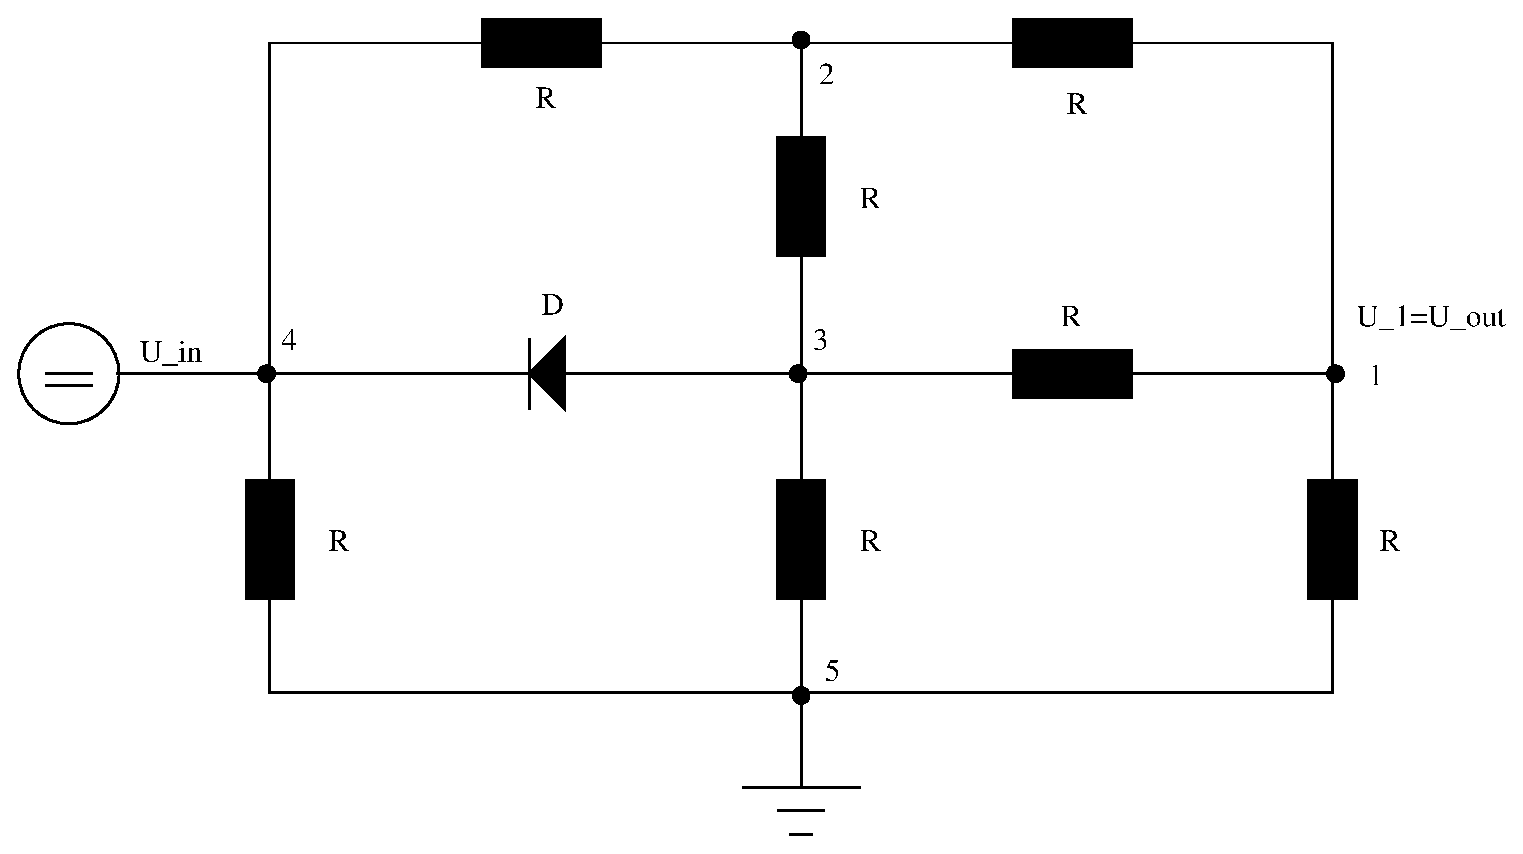
\includegraphics[scale=0.5]{\problems/ch_iterativenonlinear/PICTURES/circuit_diode.eps}
      \caption{non-linear circuit for Problem 1}
      \label{fig:circ}
    \end{figure}
    
  \begin{subproblem}[2]
    Carry out the nodal analysis of the electric circuit and
    derive the corresponding non-linear system of equations
    $\mathbf{F}(\mathbf{u})=\mathbf{0}$ for the voltages in nodes 1,2, and 3,
    \emph{cf.} \lref{eq:EMM}. Note that the voltages in nodes 4 and 5 are known
    (input voltage and ground voltage 0). 
    \begin{solution}
    We consider Kirchhoff's law $\sum\limits_{k,j} I_{kj} = 0$ for every node $k$. $I_{kj}$ contributes to the sum if node $j$
    is connected to node $k$ trough one element (R,C,L,D).
    
    \begin{itemize}
        \item[(1)] $3U_1 - 0 - U_2 - U_3=0$
        \item[(2)] $3U_2 - U_1 - U_3 - U=0$
        \item[(3)] $3U_3 - 0 - U_1 - U_2+ \alpha\Bigg(e^{\beta\Big(\frac{U_3-U}{U_T} \Big)}-1\Bigg)=0 $
    \end{itemize}
    
    Thus the nonlinear system of equations reads
    $$\mathbf{F}(\mathbf{u})=\left(\begin{array}{l}3U_1-U_2-U_3 \\ 3U_2-U_1-U_3-U \\ 
      3U_3-U_1-U_2 +\alpha e^{-\frac{\beta}{U_T}U}\cdot e^{\frac{\beta}{U_T}U_3} -\alpha \end{array}\right)=
      \left(\begin{array}{c} 0 \\0\\ 0\end{array}\right) \qquad \text{for } \mathbf{u}=\left(\begin{array}{c}U_1 \\ U_2 \\ U_3 \end{array}\right). $$
    \end{solution}
  \end{subproblem}

  \begin{subproblem}[3]
    Write an \Eigen{} function 
    \begin{lstlisting}
    void circuit(const double & alpha, const double & beta, const VectorXd & Uin, VectorXd & Uout)
    \end{lstlisting}
    that computes the output voltages \texttt{Uout} (at node 1 in Fig.~\ref{fig:circ}) for a
    \emph{sorted} vector of input voltages \texttt{Uin} (at node 4) for a thermal voltage $U_T=0.5$. The
    parameters \texttt{alpha}, \texttt{beta} pass the (non-dimensional) diode
    parameters. 

    Use Newton's method to solve $\mathbf{F}(\mathbf{u})=\mathbf{0}$ with
    a tolerance of $\tau=10^{-6}$.
      \begin{solution}
      An iteration of the multivariate Newton method is:
    $$ \mathbf{u}^{(k+1)} = \mathbf{u}^{(k)} - \big(D\mathbf{F}(\mathbf{u}^{(k)}\big)^{-1}\mathbf{F}(\mathbf{u}^{(k)}) $$
    The components of the Jacobian $D\mathbf{F}$ are defined as $D\mathbf{F}(\mathbf{u})_{ij}:=\frac{\partial F_i(\mathbf{u})}{\partial u_j}$. 
    For the function obtained in a) we get
    $$ D\mathbf{F}(\mathbf{u})=\mathbf{J}=\left(\begin{array}{rrl}3 & -1 & -1 \\ -1 & 3 & -1 \\ -1 & -1 & 3+ \frac{\alpha\beta}{U_T}e^{\beta\frac{U_3-U}{U_T}} \end{array}\right).$$
     For the implementation in Eigen see file \texttt{nonlinear\_circuit.cpp}.
            \end{solution}
  \end{subproblem}
      \begin{subproblem}[2]
      We are interested in the nonlinear effects introduced by the diode. Calculate
      $U_{\text{out}}=U_{\text{out}}(U_{\text{in}})$ as a function of the variable
      input voltage $U_{\text{in}}\in[0,20]$ (for non-dimensional parameters
      $\alpha=8$, $\beta=1$ and for a thermal voltage $U_T=0.5$) and infer the nonlinear effects from the results.
       \begin{solution}
 The nonlinear effects can be observed by calculating the differences between the solutions $U_{\text{out}}$, see file \texttt{nonlinear\_circuit.cpp}.
       \end{solution}
    \end{subproblem}
  \end{problem}
 % ncse_new/p1_SystemsOfEquations/ch3_IterativeMethodsNonLinear/ex_JuliaSet.tex
% solutions:       ex_JuliaSet_20_1000.pdf        julia_set.m

\begin{problem}[Julia set]

\href{http://en.wikipedia.org/wiki/Julia_set}{Julia sets} are famous fractal
shapes in the complex plane.  They are constructed from the basins of attraction
of zeros of complex functions when the Newton method is applied to find them.
%In this problem we aim to visualize a Julia set.

In the space $\bbC$ of complex numbers the equation
\begin{equation}\label{eq:root_of_1} z^3=1 \end{equation}
has three solutions: $z_{1}=1$,
$z_{2}=-\frac{1}{2}+\frac{1}{2}\sqrt{3}i$,
$z_{3}=-\frac{1}{2}-\frac{1}{2}\sqrt{3}i$ (the cubic roots of unity).


\begin{subproblem}[2] \label{subprb:JuliaSet_1}
As you know from the analysis course, the complex plane $\bbC$ can be identified
with $\bbR^{2}$ via $(x,y)\mapsto z=x+iy$. Using this identification, convert
equation (\ref{eq:root_of_1}) into a system of equations $\VF(x,y) = \Vzero$ for a
suitable function $\VF:\bbR^{2}\mapsto\bbR^{2}$.

\begin{solution}
We have $$z^3 - 1 =(x+iy)^3 -1 = x^3+3ix^2y-3xy^2-iy^3-1 = x^3-3xy^2-1+i(3x^2y-y^3)=0.$$
Thus, equation \eqref{eq:root_of_1} is equivalent to
$\quad \mathbf{F}(x,y)=\left(\begin{array}{c}x^3-3xy^2-1 \\ 3x^2y-y^3\end{array}\right)=\left(\begin{array}{c}0\\0\end{array}\right).$
\end{solution}
\end{subproblem}

\begin{subproblem}[3] \label{subprb:JuliaSet_2}
Formulate the Newton iteration \lref{eq:Newton} for the non-linear equation $\VF(\Vx) =\Vzero$ with $\Vx = (x,y)^{T}$ and $\VF$ from the previous sub-problem.

\begin{solution}
The iteration of Newton's method for multiple variables reads
$$\mathbf{x}^{(k+1)} = \mathbf{x}^{(k)}-\big(D\mathbf{F}(\mathbf{x}^{(k)})\big)^{-1}\mathbf{F}(\mathbf{x}^{(k)}),$$
where $D\mathbf{F}$ is the Jacobian
$D\mathbf{F}(\mathbf{x})=\left(\begin{array}{cc} 3x^2-3y^2&-6xy\\ 6xy&3x^2-3y^2 \end{array}\right)$.
\end{solution}
\end{subproblem}

\begin{subproblem}[4] \label{subprb:JuliaSet_3}
Denote by $\Vx^{(k)}$ the iterates produced by the Newton method from the previous sub-problem with some initial vector $\Vx^{(0)}\in\bbR^{2}$.
Depending on $\Vx^{(0)}$, the sequence $\Vx^{(k)}$ will either diverge or converge to one of the three cubic roots of unity.

    Analyze the behavior of the Newton iterates using the following procedure:
    \begin{itemize}
    \item use equally spaced points on the domain $[-2,2]^2\subset\bbR^2$ as starting points of the Newton iterations,
    \item color the starting points differently depending on which of the three roots is the limit of the sequence $\Vx^{(k)}$.
 %         For instance you can create a RGB colormap .......... (a fourth color for diverging sequences).
    \end{itemize}

    \hint: useful \Matlab commands: \texttt{pcolor}, \texttt{colormap},
    \texttt{shading}, \texttt{caxis}. You may stop the iteration once you are
    closer in distance to one of the third roots of unity than $10^{-4}$.

The three (non connected) sets of points whose iterations are converging to the different $z_i$ are called Fatou domains, their boundaries are the Julia sets.

\begin{solution}
For each starting point at most \texttt{N\_it} iterations are accomplished.
For a given starting point $\mathbf{x}^{(0)}$, as soon as the condition $|{x}^{(k)}_1+i{x}^{(k)}_2-z_i| < 10^{-4},\; i\in\{1,2,3\}$ is reached, we assign a color depending on the root $z_i$ and on the number of iterations done.
Each attractor is associated to red, green or blue; lighter colors correspond to the points with faster convergence.
The points that are not converging in \texttt{N\_it} iterations are white.
We set the color scale using the \Matlab commands \texttt{colormap} and \texttt{caxis}.

%        \begin{figure}[hbt]   \begin{center}
%        \includegraphics[width=0.6\textwidth]{ex_JuliaSet_25_1000}
%        \caption{Julia set for $z^3-1=0$ on a mesh containing $1000\times1000$ points, \texttt{N\_it}=25.}
%        \end{center} \end{figure}

    \begin{figure}[hbt]   \begin{center}
        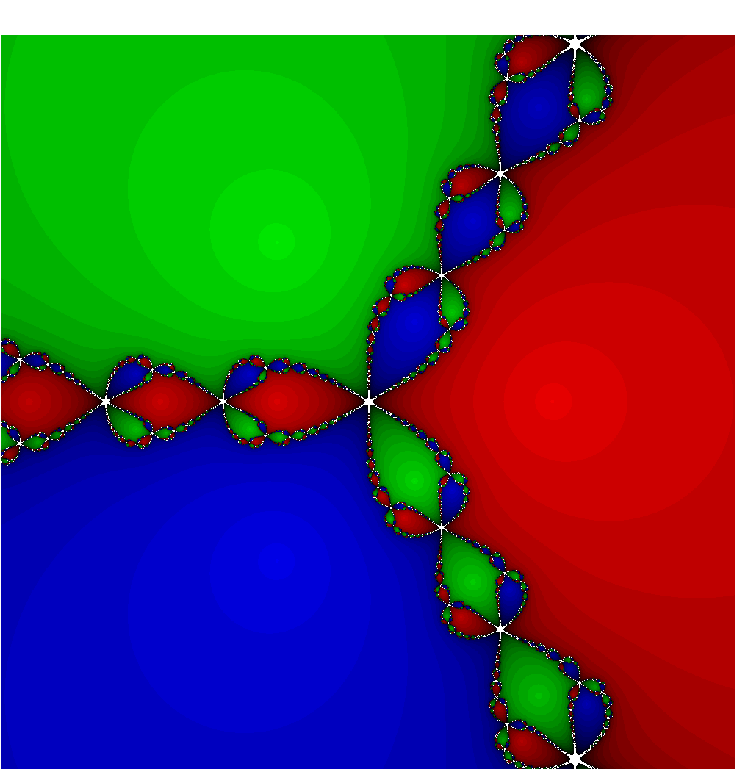
\includegraphics[width=0.6\textwidth]{\problems/ch_iterativenonlinear/PICTURES/ex_JuliaSet_20_1000.pdf} % tille: changed to pdf for better compression
        \caption{Julia set for $z^3-1=0$ on a mesh containing $1000\times1000$ points, \texttt{N\_it}=20.}
        \end{center} \end{figure}

\lstinputlisting[caption={\texttt{julia\_set.m}}, label={mc:julia_set}]
{\problems/ch_iterativenonlinear/MATLAB/julia_set.m}
\end{solution}
\end{subproblem}
\end{problem}

\end{sheet}

%%% PS6
\begin{sheet}{6}{22.10.2015}{29.10.2015}
% ncse_new/p2_InterpolationApproximation/ch1_PolynomialInterpolation/ex_EvaluatingDerivatives.tex
% exercise requires:    -
% solutions require:    dipoleval.m  dipoleval_test.m  dipoleval_test.eps

\begin{problem}[Evaluating the derivatives of interpolating polynomials \coreproblem]
\label{prb:EvaluatingDerivatives}

In \lref{sec:polipsingleeval} we learned about an efficient and
``update-friendly'' scheme for evaluating Lagrange interpolants at a single or a
few points. This so-called Aitken-Neville algorithm, see \lref{AitkenNeville}, can
be extended to return the derivative value of the polynomial interpolant as well.
This will be explored in this problem. 

\begin{subproblem}[1]
  Study the Aitken-Neville scheme introduced in \lref{par:AIN}. 
\end{subproblem}

\begin{subproblem}[3]\label{dpe:sp:1}
Write an efficient MATLAB function
\begin{center}
\texttt{dp = dipoleval(t,y,x)}
\end{center}
that returns the row vector $(p'(x_{1}),\ldots,p'(x_{m}))$, when the argument
\texttt{x} passes $(x_{1},\ldots,x_{m})$, $m\in\bbN$ small.  Here, $p'$ denotes the
\emph{derivative} of the polynomial $p\in\Pol{n}$ interpolating the
data points $(t_{i},y_{i})$, $i=0,\ldots,n$, for pairwise different
$t_{i}\in\bbR$ and data values $y_{i}\in\bbR$.

\begin{hint}
Differentiate the recursion formula \lref{eq:ipolrec} and
devise an algorithm in the spirit of the Aitken-Neville algorithm
implemented in \lref{AitkenNeville}.
\end{hint}

\begin{solution}
Differentiating the recursion formula \ncseeq{eq:ipolrec} we obtain
%
\begin{equation*}
\begin{aligned}
p_i(t) &\equiv y_i, \qquad i = 0, \dots, n, \\
p'_i(t) &\equiv 0, \qquad i = 0, \dots, n, \\
p_{i_0,\dots,i_m}(t) &= \frac{ (t-t_{i_0}) p_{i_1,\dots,i_m}(t) - (t-t_{i_m}) p_{i_0,\dots,i_{m-1}}(t) }{t_{i_m}-t_{i_0}}, \\
p'_{i_0,\dots,i_m}(t) &= \frac
{ p_{i_1,\dots,i_m}(t) + (t-t_{i_0}) p'_{i_1,\dots,i_m}(t) - p_{i_0,\dots,i_{m-1}}(t) - (t-t_{i_m}) p'_{i_0,\dots,i_{m-1}}(t) } {t_{i_m}-t_{i_0}}.
\end{aligned}
\end{equation*}
%
The implementation of the above algorithm is given in file \texttt{dipoleval\_test.m}.
\end{solution}
\end{subproblem}

\begin{subproblem}[2]
  For validation purposes devise an alternative, less efficient, implementation of
  \texttt{dipoleval} (call it \texttt{dipoleval\_alt}) based on the following
  steps:
  \begin{enumerate}
  \item Use \matlab{}'s \texttt{polyfit} function to compute the monomial
    coefficients of the Lagrange interpolant.
  \item Compute the monomial coefficients of the derivative.
  \item Use \texttt{polyval} to evaluate the derivative at a number of points.
  \end{enumerate}
  Use \texttt{dipoleval\_alt} to verify the correctness of your implementation of
  \texttt{dipoleval} with \texttt{t = linspace(0,1,10)}, \texttt{y = rand(1,n)}
  and \texttt{x = linspace(0,1,100)}.

\begin{solution}
See file \texttt{dipoleval\_test.m}.

% We verify the correctness of the implementation in \autoref{mc:EvaluatingDerivatives_dipoleval_test}.
% See \autoref{fig:EvaluatingDerivatives_dipoleval_test} for the results.
% %
% \lstinputlisting[label={mc:EvaluatingDerivatives_dipoleval_test},caption={Implementation of \texttt{dipoleval\_test}}]
% {\problems/ch_polynomialinterpolation/MATLAB/dipoleval_test.m}
% %
% \begin{figure}[ht]
% \centering
% \includegraphics[width=0.8\textwidth]{\problems/ch_polynomialinterpolation/PICTURES/dipoleval_test.eps}
% \caption{Testing routine \texttt{dipoleval} by comparing to divided differences}
% \label{fig:EvaluatingDerivatives_dipoleval_test}
% \end{figure}
\end{solution}
\end{subproblem}
\end{problem}

\begin{problem}[Piecewise linear interpolation]
  \lref{ex:pwlin} introduced piecewise linear interpolation as a simple linear
  interpolation scheme. It finds an interpolant in the space spanned by the
  so-called tent functions, which are \emph{cardinal basis functions}. Formulas
  are given in \lref{eq:pwlinbas}. 

% Recall that given a vector of nodes $t_i$, 
%   $i = 0, \dots, n$ ($t_i \neq t_j, i \neq j$), the tent functions $b_i$ satisfy:
%  \begin{itemize}
%   \item the basis is local:
%   \[
% \supp b_i = \{ x \in \IR \; b_i(x) = 0 \} = (t_{i-1}, t_{i+1});
%   \]
%   \item the basis is cardinal:
%   \[
%     b_i(t_j) = \delta_{i,j} = \begin{cases} 1 & i = j \\ 0 & i \neq j \end{cases};
%   \]
%   \item $b_i$ is piecewise linear in $[t_j, t_{j+1}], \forall j$;
%  \end{itemize}
%  We can then define the piecewise linear interpolant $\ell$ to be a linear combination of the basis functions $b_i: \IR \rightarrow \IR$:
%  \[
%   \ell = \sum_{i = 0}^n y_i b_i, c_i \in \IR
%  \]
%  we call $c_i$ the coefficients of the representation of $\ell$ in the basis
%  $\{ b_i \}$. Notice that an interpolant is well defined, if we provide values at
%  each node, i.e. if we provide the data $(t_i, y_i)$.

%  
%  \begin{subproblem}[1]
%   Think on how to represent the basis in memory.
%   
% \cprotEnv \begin{solution}
%    See \verb|linearinterpolant.cpp|.
%   \end{solution}
%  \end{subproblem}
%  
 \begin{subproblem}[3]
  Write a \Cpp{} class \verb|LinearInterpolant| representing the piecewise linear interpolant. Make sure your class has an efficient internal representation of a basis. Provide a constructor and an evaluation \verb|operator()| as described in the following template:
  \begin{lstlisting}[language=c++]
class LinearInterpolant {
    public:
        LinearInterpolant( /*  TODO: pass pairs */) {
	    // TODO: construct your data from  (t_i, y_i)'s
        }
        
        double operator() (double x) {
            // TODO: return I(x)
        }
    private:
        // Your data here
};
  \end{lstlisting}
  
  \begin{hint}
   Recall that \Cpp{} provides containers such as \verb|std::vector| and \verb|std::pair|.
  \end{hint}

\cprotEnv \begin{solution}
   See \verb|linearinterpolant.cpp|.
  \end{solution}
\end{subproblem}

 \begin{subproblem}[1]
  Test the correctness of your code.
 \end{subproblem}
 
\end{problem}

% ncse_new/p2_InterpolationApproximation/ch1_PolynomialInterpolation/ex_EvaluatingDerivatives.tex
% exercise requires:    -
% solutions require:    dipoleval.m  dipoleval_test.m  dipoleval_test.eps

\begin{problem}[Evaluating the derivatives of interpolating polynomials \coreproblem]
\label{prb:EvaluatingDerivatives}
This problem is about the Horner scheme, that is a way to efficiently evaluate a polynomial in a given point, see \lref{rem:Horner-scheme}.
\begin{subproblem}[3]
Using the Horner scheme, write an efficient C++ implementation of a function
\begin{lstlisting}
template <typename CoeffVec>
std::pair<double,double> evaldp ( const CoeffVec & c, double x )
\end{lstlisting}
which returns the pair $(p(x),p'(x))$, where $p$ is the polynomial with coefficients in \texttt{c}. The vector \texttt{c} contains the coefficient of the polynomial in the monomial basis, using Matlab convention (leading coefficient in \texttt{c[0]}).
\begin{solution}
See file \texttt{horner.cpp}.
\end{solution}
\end{subproblem}
\begin{subproblem}[2]
  For the sake of testing, write a naive C++ implementation of the above function
\begin{lstlisting}
template <typename CoeffVec>
std::pair<double,double> evaldp_naive ( const CoeffVec & c, double x )
\end{lstlisting}
which returns the same pair $(p(x),p'(x))$. This time, $p(x)$ and $p'(x)$ should be calculated with the simple sums of the monomials constituting the polynomial.
\begin{solution}
See file \texttt{horner.cpp}.
\end{solution}
\end{subproblem}
\begin{subproblem}[1]
What are the asymptotic complexities of the two implementations?
\begin{solution}
  In both cases, the algorithm requires $\approx n$ multiplications and additions,
  and so the asymptotic complexity is $O(n)$. The naive implementation also calls
  the \texttt{pow()} function, which may be costly. 
\end{solution}
\end{subproblem}
\begin{subproblem}[1]
Check the validity of the two functions and compare the runtimes for polynomials of degree up to $2^{20}-1$.
\begin{solution}
See file \texttt{horner.cpp}.
\end{solution}
\end{subproblem}
\end{problem}

\begin{problem}[Lagrange interpolant]
 
 Given data points $(t_i, y_i)_{i = 1}^n$, show that the Lagrange interpolant
 \[
  p(x) = \sum_{i = 0}^n y_i L_i(x), \quad L_i(x) := \prod_{\substack{j = 0\\ j \neq i}}^n \frac{x - t_j}{t_i - t_j}
 \]

 is given by:
 \[
  p(x) =  \omega(x)  \sum_{j = 0}^n \frac{y_j}{(x-t_j) \omega' (t_j)}
 \]
 with $\omega(x) = \prod_{j = 0}^n (x - t_j)$.
 
 \begin{solution}
 Simply exploiting the chain rule of many terms:
  \[
   \omega'(x) = \sum_{i = 0}^n \prod_{\substack{j = 0\\ j \neq i}}^n (x - t_j)
  \]
  Since $(t_i - t_j) = \delta_{i,j}$, it follows $\omega'(t_i) = \prod_{\substack{j = 0\\ j \neq i}}^n (t_i - t_j)$.
  Therefore:
  \begin{align*}
  p(x) =  \omega(x)  \sum_{j = 0}^n \frac{y_j}{(x-t_j) \omega' (t_j)} = \sum_{j = 0}^n \frac{y_j}{(x-t_j) \prod_{\substack{j = 0\\ j \neq i}}^n (t_i - t_j)} \prod_{j = 0}^n (x - t_j) \\
= \sum_{j = 0}^n \frac{y_j}{\prod_{\substack{j = 0\\ j \neq i}}^n (t_i - t_j)} \prod_{\substack{j = 0\\ j \neq i}}^n (x - t_j) = \sum_{j = 0}^n y_j \prod_{\substack{j = 0\\ j \neq i}}^n \frac{x - t_j}{t_i - t_j}.
  \end{align*}


 \end{solution}

 
\end{problem}

\end{sheet}

%%% PS7
\begin{sheet}{7}{29.10.2015}{05.11.2015}
% ncse_new/\problems/ch_piecewisepolynomials/ex_CubicSplines.tex
%  solution:  ex_CubicSpline.m  ex_CubicSpline.eps

\begin{problem}[Cubic Splines \coreproblem] \label{prb:CubicSplines}
  Since they mimic the behavior of an elastic rod pinned at fixed points, see
  \lref{rem:csrod}, cubic splines are very popular for creating ``aesthetically
  pleasing'' interpolating functions. However, in this problem we look at a
  cubic spline from the perspective of its defining properties, see
  \lref{def:spline}, in order to become more familiar with the concept of
  spline function and the consequences of the smoothness required %stipulated
  by the definition.

 For parameters $\alpha,\beta\in\bbR$ we define the function
  $s_{\alpha,\beta}:[-1,2]\to \bbR$ by
  \begin{gather}    \label{eq:ex_CubicSplines}
    s_{\alpha,\beta}(x) = \left\{\begin{array}{ll}
        (x+1)^4+\alpha(x-1)^4+1 & x\in[-1,0]\\
        -x^3-8\alpha x +1 &       x\in(0,1]\\
        \beta x^3+8x^2 + \frac{11}{3} & x\in(1,2]
      \end{array}\right.
  \end{gather}


% interesting alternative choice!!!
% define s(x) = x^3+x^2+6+\beta(x-1)^2   in the 3rd interval
% it is C^1 for every beta, C^2 only for beta = -7
% they can play with the plot and see 2nd derivatives as curvature
% matlab line:   y3 = x3.^3 + x3.^2 + 6 + beta*( x3-1 ).^2;


%=====================================================================================================
\begin{subproblem}[2] \label{subprb:CubicSplines_1}     % a
    Determine $\alpha,\beta$ such that $s_{\alpha,\beta}$ is a cubic spline in $\Cs_{3,M}$
    with respect to the node set $M=\{-1,0,1,2\}$.
    Verify that you actually obtain a cubic spline.

    %\Hint: The continuity conditions for $s$, $s'$, and $s''$ have to hold at internal nodes.

\begin{solution}
We immediately see that $\alpha=-1$ is necessary to get a polynomial of $3^{\text{rd}}$ degree.

Furthermore, from the condition
$$8=s_{-1,\beta}(1^-)=s_{-1,\beta}(1^+)=\beta+8+\frac{11}{3}\qquad
\text{we get }\quad\beta=-\frac{11}{3}.$$
It remains to check the continuity of $s,s',s''$ in the nodes $0$ and $1$. Indeed, we have
$$s_{-1,\beta}'(x)=
\begin{cases}
4(x+1)^3+4\alpha(x-1)^3   \\
-3x^2-8\alpha             \\
3\beta x^2+16x
\end{cases}
s_{-1,\beta}''(x)
\begin{cases}
 12(x+1)^2+12\alpha(x-1)^2  &-1\le x\le0,\\
 -6x  & 0<x\le 1,\\
6\beta x+16 & 1<x<2.
\end{cases}$$
Therefore the values in the nodes are

\begin{tabular}{  c | c c | c c | }%\hline
 & $0^-$ & $0^+$ & $1-$ & $1^+$\\ \hline
$s$ & $2+\alpha$ & 1 & $-8\alpha$ & $\beta+8+11/3$\\
$s'$ & $4-4\alpha$ & $-8\alpha$ & $-3-8\alpha$ & $3\beta+16$\\
$s''$ & $12+12\alpha$ & 0 & -6 & $6\beta+16$%\\ \hline
\end{tabular}
$\begin{matrix}
\alpha=-1, \\ \beta=-11/3\rightarrow
\end{matrix}$
\begin{tabular}{  c | c c | c c | }%\hline
 & $0^-$ & $0^+$ & $1-$ & $1^+$\\ \hline
$s$ & 1 & 1 & 8 & 8\\
$s'$ & 8 & 8 & 5 & 5\\
$s''$ & 0 & 0 & -6 & -6%\\ \hline
\end{tabular}

They agree for our choice of the parameters.
% \[ \begin{array}{rclrcl}
% s_{\alpha,\beta}(0^-)&=&2+\alpha=1 & s_{\alpha,\beta}(0^+)&=&1\\ s_{\alpha,\beta}(1^-)&=&-8\alpha=8 & s_{\alpha,\beta}(1^+)&=&\beta+\frac{35}{3} =8
% \end{array} \]
% \[ \begin{array}{rclrcl}
% s_{\alpha,\beta}'(0^-)&=&4(1-\alpha)=8 & s_{\alpha,\beta}'(0^+)&=&-8\alpha=8\\ s_{\alpha,\beta}'(1^-)&=&-3-8\alpha=5 & s_{\alpha,\beta}'(1^+)&=&3\beta+16 =5
% \end{array} \]
% \[ \begin{array}{rclrcl}
% s_{\alpha,\beta}''(0^-)&=&12+12\alpha=0 & s_{\alpha,\beta}''(0^+)&=&0\\ s_{\alpha,\beta}''(1^-)&=&-6 & s_{\alpha,\beta}''(1^+)&=&6\beta+16 =-6
% \end{array} \]
\end{solution}
\end{subproblem}


%=====================================================================================================

\begin{subproblem}[1] \label{subprb:CubicSplines_2}     % a
    Use \Matlab{} to create a plot of the function defined in \eqref{eq:ex_CubicSplines} in dependance of $\alpha$ and $\beta$.

\begin{solution}
\lstinputlisting[caption={Matlab Code for \texttt{Cubic Spline}},label={lst:cub_spline}]
 {\problems/ch_piecewisepolynomials/MATLAB/ex_CubicSpline.m}

\begin{center}
  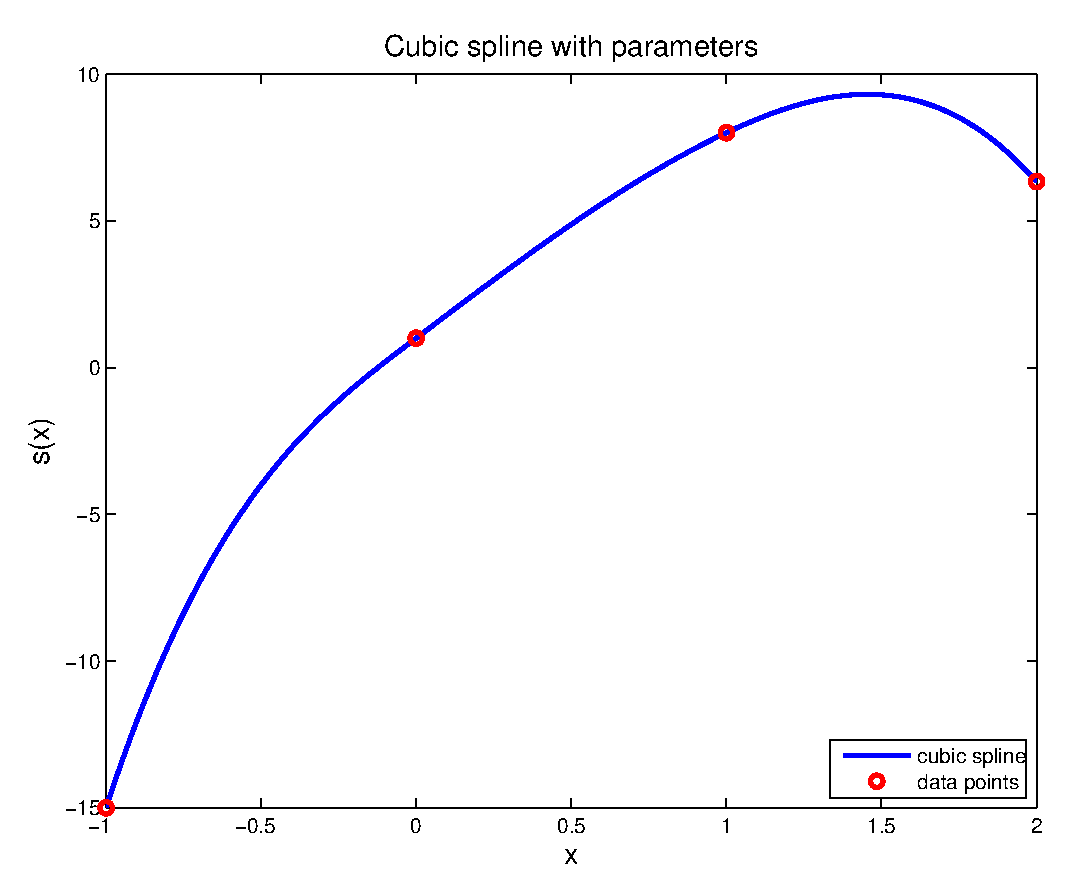
\includegraphics[width=0.5\textwidth]{\problems/ch_piecewisepolynomials/PICTURES/ex_CubicSpline.eps}
\end{center}

\end{solution}
\end{subproblem}
\end{problem}




	
% ncse_new/p2_InterpolationApproximation/ch2_PiecewisePolynomials/ex_QuadraticSplines.tex
% exercise requires:   quadspline_p.p
% solutions require:   quadspline.m  ex_QuadraticSplinesPlot.m  interpol_quad_T2.eps  ex_QuadraticSplinesConv.m  time-error_QuadSplines.eps


\begin{problem}[Quadratic Splines \coreproblem] \label{prb:QuadraticSplines}

\lref{def:spline} introduces spline spaces $\Cs_{d,\Cm}$ of any degree
{$d\in\bbN_{0}$} on a node set $\Cm\subset\bbR$. \lref{sec:csi} discusses
interpolation by means of cubic splines, which is the most important case.
In this problem we practise spline interpolation for quadratic splines
in order to understand the general principles.

Consider a 1-periodic function $f: \mathbb{R} \rightarrow \mathbb{R}$, that is,
$f(t+1)=f(t)$ for all $t\in\bbR$, and a set of nodes
\begin{gather*}%    \label{eq:2}
\mathcal{M}:=\{0=t_0<t_{1}<t_{2}<\dots<t_{n-1}<t_n=1\}\subset[0,1]\;.
\end{gather*}
We want to approximate $f$ using a \emph{1-periodic} quadratic spline function
$s\in\Cs_{2,\Cm}$, which interpolates $f$ \emph{in the midpoints} of the intervals
$[t_{j-1},t_{j}]$, $j=0,\ldots,n$.

In analogy to the local representation of a cubic spline function according to
\lref{cs:rep}, we parametrize a quadratic spline function
$s\in\mathcal{S}_{2,\Cm}$ according to
\begin{gather} \label{eq:quad_spl}
s|_{[t_{j-1},t_{j}]}(t) = d_{j}\;\tau^{2} + c_{j}\;4\;\tau(1-\tau) + d_{j-1}\;(1-\tau)^{2}\;,
\quad \tau := \frac{t-t_{j-1}}{t_{j}-t_{j-1}}\;,\quad
j=1,\ldots,n\;,
\end{gather}
with $c_j,d_k\in\bbR$, $j=1,\ldots,n,\; k=0,\ldots,n$.
Notice that the coefficients $d_k$ are associated with the nodes $t_k$ while the $c_j$ are associated with the midpoints of the intervals $[t_{j-1},t_j]$.


% ================= SUBPROBLEM 1

\begin{subproblem}[1] \label{subprb:QuadraticSplines_1}
What is the dimension of the subspace of \emph{1-periodic} spline functions in $\Cs_{2,\Cm}$?

\begin{solution} Counting argument, similar to that used to determine the
  dimensions of the spline spaces. We have $n+1$ unknowns $d_k$ and $n$ unknowns
  $c_j$, the constraint $d_0=s(t_0) = s(t_0+1) = s(t_n) = d_n$ leaves us with a
  total of $2n$ unknowns.  The continuity of the derivatives in the $n$ nodes
  impose the same number of constraints, therefore the total dimension of the
  spline space is $2n-n=n$.
\end{solution}
\end{subproblem}

% ================= SUBPROBLEM 2

\begin{subproblem}[1]  \label{subprb:QuadraticSplines_2}
What kind of continuity is already guaranteed by the use of the representation \eqref{eq:quad_spl}?

% need more explanations: student from last year assumed that C_1 is guaranteed since we _enforce_ it...

\begin{solution}
 We observe that $s(t_j^-)=s|_{[t_{j-1},t_{j}]}(t_j) = d_j = s|_{[t_{j},t_{j+1}]}(t_j)=s(t_j^+)$, thus we get continuity for free.
However the derivatives do not necessarily match.
\end{solution}
\end{subproblem}

% ================= SUBPROBLEM 3

\begin{subproblem}[3]  \label{subprb:QuadraticSplines_3} 
    Derive a linear system of equations (system matrix and right hand side) whose
    solution provides the coefficients $c_{j}$ and $d_{j}$ in \eqref{eq:quad_spl} from the
    function values $y_{j} := f(\frac{1}{2}(t_{j-1}+t_{j}))$, $j=1,\ldots,n$.

    \hint{} By \lref{def:spline} we know $\Cs_{2,\Cm}\subset C^{1}([0,1])$,
    which provides linear constraints at the nodes, analogous to \lref{cs:cc} for
    cubic splines.


\begin{solution}
We can plug $t = \frac{1}{2}(t_j + t_{j-1})$ into \eqref{eq:quad_spl}
and set the values equal to $y_j$. We obtain $\tau=1/2$ and the following conditions:
\begin{equation}\label{matching_y}
 \frac{1}{4} d_j + c_j + \frac{1}{4} d_{j-1} = y_j,\quad j=1,...,n.
\end{equation}
We obtain conditions on $d_j$ by matching the derivatives at the interfaces.
The derivative of the quadratic spline can be computed from \eqref{eq:quad_spl}, after defining $\Delta_j=t_j-t_{j-1}$:
$$s'|_{[t_{j-1},t_{j}]}(t)=\Delta_j^{-1}\frac{\partial}{\partial \tau}\Big( \tau^{2}d_{j} + 4\tau(1-\tau)c_{j} + (1-\tau)^{2}d_{j-1}\Big)
=\Delta_j^{-1}\Big(2\tau d_j+4(1-2\tau)c_j-2(1-\tau)d_{j-1}\Big).$$
Setting $\tau=1$ in $[t_{j-1},t_j]$ and  $\tau=0$ in $[t_j,t_{j+1}]$,
the continuity of the derivative in the node $t_j$ enforces the condition
$$\frac{2d_j-4c_j}{\Delta_j}
= s'|_{[t_{j-1},t_{j}]}(t_j)
= s'(t_j^-) = s'(t_j^+)
= s'|_{[t_{j-1},t_{j}]}(t_j)
= \frac{4c_{j+1}-2d_j}{\Delta_{j+1}}; $$
(this formula holds for $j=1,\ldots,n$ if we define $t_{n+1}=t_1+1$ and $c_{n+1}=c_1$).
Simplifying for $d_j$ we obtain:
\begin{align*}
d_j & = \frac{2\frac{c_j}{\Delta_j}+2\frac{c_{j+1}}{\Delta_{j+1}}}{\frac1{\Delta_j}+\frac1{\Delta_{j+1}}}
      = 2\frac{c_j\Delta_{j+1}+c_{j+1}\Delta_j}{\Delta_j+\Delta_{j+1}}
      = 2\frac{c_j(t_{j+1}-t_j)+c_{j+1}(t_j-t_{j-1})}{t_{j+1}-t_{j-1}},\qquad j=1,\ldots,n.
\end{align*}
Plugging this expression into \eqref{matching_y}, we get the following system of equations:
\begin{equation}\label{sys_eq_c_full}
\frac{1}{2}\frac{c_{j+1}(t_{j}-t_{j-1}) + c_j(t_{j+1}-t_j)}{t_{j+1}-t_{j-1}}
+ c_j + \frac{1}{2}\frac{c_{j}(t_{j-1}-t_{j-2}) + c_{j-1}(t_{j}-t_{j-1})}{t_{j}-t_{j-2}} = y_j,\qquad j=1,\ldots,n,
\end{equation}
with the periodic definitions $t_{-2} = t_{n-2}-1$, $c_0 = c_n$, $c_{-1} = c_{n-1}$.
We collect the coefficients and finally we obtain
\begin{equation}\label{simplif_eq_c}
\underbrace{\left\{\frac{1}{2} \frac{t_j-t_{j-1}}{t_j-t_{j-2}}\right\}}_{A_{j-1}} c_{j-1} +
\underbrace{\left\{\frac{1}{2} \frac{t_{j+1}-t_{j}}{t_{j+1}-t_{j-1}} + 1
  + \frac{1}{2} \frac{t_{j-1}-t_{j-2}}{t_{j}-t_{j-2}}\right\}}_{B_{j}} c_{j}
+ \underbrace{\left\{\frac{1}{2} \frac{t_j-t_{j-1}}{t_{j+1}-t_{j-1}}\right\}}_{C_{j+1}} c_{j+1} = y_j,\quad j=1,\ldots,n.
\end{equation}
If we have an equidistant grid with $t_j - t_{j-1} = 1/n$, this simplifies to
\begin{equation*}%\label{equi_simpl_eq_c}
 \frac{1}{4}c_{j-1} + \frac{3}{2} c_j + \frac{1}{4} c_{j+1} = y_j,\qquad \qquad j=1,\ldots,n.
\end{equation*}
The system of equations in matrix form looks as follows:
\begin{equation}\label{system}
 \begin{pmatrix}
  B_1 & C_2 & 0 & 0 & 0 & \cdots \cdots & 0 & 0 & 0 & A_0\\
  A_1 & B_2 & C_3 & 0 & 0 & \cdots \cdots & 0 & 0 & 0 & 0 \\
  0 & A_2 & B_3 & C_4 & 0 & \cdots \cdots & 0 & 0 & 0 & 0 \\
  \vdots & \vdots & \ddots & \ddots & \ddots &  & \vdots & \vdots & \vdots & \vdots \\
  \vdots & \vdots & \vdots & \ddots & \ddots & \ddots & \vdots & \vdots & \vdots & \vdots \\
  \vdots & \vdots & \vdots & \vdots & \ddots & \ddots & \ddots & \vdots & \vdots & \vdots \\
  \vdots & \vdots & \vdots & \vdots & \vdots& \ddots & \ddots & \ddots & \vdots & \vdots \\
  \vdots & \vdots & \vdots & \vdots & \vdots & & \ddots & \ddots & \ddots & 0 \\
  0 & 0 & 0 & 0 & 0 & \cdots \cdots & 0 & A_{n-2} & B_{n-1} & C_n \\
  C_{n+1} & 0 & 0 & 0 & 0 & \cdots \cdots & 0 & 0 & A_{n-1} & B_n \\
 \end{pmatrix}
 \begin{pmatrix}c_1\\c_2\\c_3\\\vdots\\\vdots\\\vdots\\\vdots\\\vdots\\c_{n-1}\\c_n\end{pmatrix}
=\begin{pmatrix}y_1\\y_2\\y_3\\\vdots\\\vdots\\\vdots\\\vdots\\\vdots\\y_{n-1}\\y_n\end{pmatrix}.
\end{equation}
\end{solution}
\end{subproblem}

% ================= SUBPROBLEM 4

\begin{subproblem}[3]  \label{subprb:QuadraticSplines_4}
Implement an \emph{efficient} \Matlab{} routine
\begin{center}
  \texttt{function s=quadspline(t,y,x)}
\end{center}
which takes as input
a (sorted) node vector \texttt{t} (of length $n-1$, because $t_{0}=0$ and $t_{n}=1$ will be taken for granted),
a $n$-vector \texttt{y} containing the values of a function $f$ at the midpoints $\frac{1}{2}(t_{j-1}+t_{j})$, $j=1,\ldots,n$,
and a \emph{sorted} $N$-vector \texttt{x} of evaluation points in $[0,1]$.

The function is to return the values of the interpolating quadratic spline $s$ at
the positions \texttt{x}.

You can test your code with the one provided by \texttt{quadspline\_p.p} (available on the lecture website).

\begin{solution}
See \autoref{mc:quadspline}.
\lstinputlisting[caption={Construction of the quadratic spline and evaluation.},label={mc:quadspline}, escapechar={}]
{\problems/ch_piecewisepolynomials/MATLAB/quadspline_better.m}

It is important not to get lost in the indexing of the vectors. In this code they can be represented as:\\
{\tt t=(t1, t2, ..., t\{n-1\})} \quad length $=n-1$,\\
{\tt ext\_t=(t\{n-1\}-1, t0=0, t1, t2,..., t\{n-1\}, tn=1, 1+t1)}\quad length $=n+3$,\\
{\tt de\_t=(1-t\{n-1\}, t1, t2-t1,..., t\{n-1\}-t\{n-2\}, 1-t\{n-1\}, t1)}\;,\\
{\tt dde\_t=(t1+1-t\{n-1\}, t2, t3-t1,..., 1-t\{n-2\}, t1+1-t\{n-1\})}\;.\\
The vectors \texttt{A,B,C,c,d} have length $n$ and correspond to the definitions given in \ref{subprb:QuadraticSplines_3} (with the indexing from 1 to $n$).
\end{solution}
\end{subproblem}

% ================= SUBPROBLEM 5

\begin{subproblem}[1] \label{subprb:QuadraticSplines_5} Plot $f$ and the
  interpolating periodic quadratic spline $s$ for $f(t) := \exp(\sin(2\pi t))$,
  $n=10$ and $\Cm = \left\{\frac{j}{n}\right\}_{j=0}^{10}$, that is, the spline is
  to fulfill $s(t)=f(t)$ for all midpoints $t$ of knot intervals.

\begin{solution}See code \ref{mc:quadspline_plot} and Figure \ref{fig:interpol_quad_T2}.
\lstinputlisting[caption={Plot of the quadratic splines.},label={mc:quadspline_plot}, escapechar={}]
{\problems/ch_piecewisepolynomials/MATLAB/ex_QuadraticSplinesPlot.m}
\begin{figure}[htb]
\caption{Quadratic spline interpolation of $f$ in 10 equispaced nodes.}\label{fig:interpol_quad_T2}
\centering 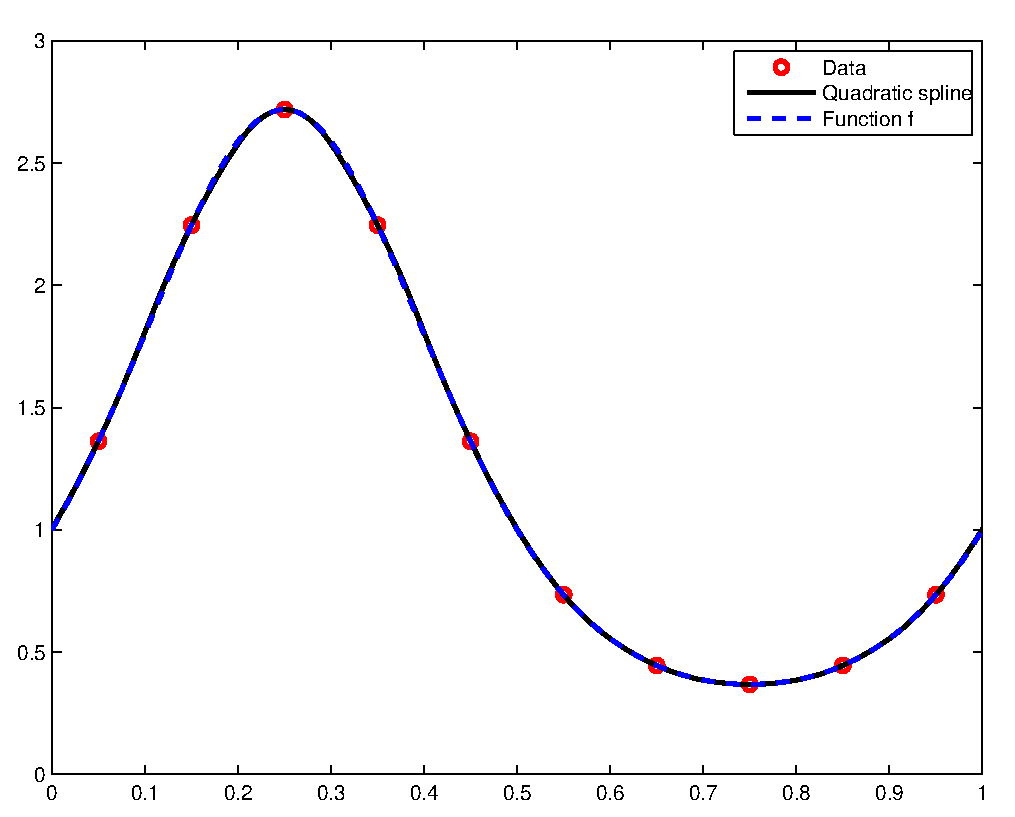
\includegraphics[width = 0.6 \textwidth]{\problems/ch_piecewisepolynomials/PICTURES/interpol_quad_T2.eps}
\end{figure}
\end{solution}
\end{subproblem}

% \subproblem\label{subprb:QuadraticSplines_7}
% What is the asymptotic complexity of your implementation of \texttt{quadspline}
% for \emph{fixed} $n$ and $N\to\infty$?
%
% \begin{solution}The evaluation is $\mathcal{O}(N)$.}

% ================= SUBPROBLEM 6

\begin{subproblem}[1]  \label{subprb:QuadraticSplines_6}
What is the complexity of the algorithm in \ref{subprb:QuadraticSplines_4} in dependance of $n$ and $N$?

\begin{solution}
The complexity is linear both in $N$ (sequential evaluation in different points) and in $n$, provided one exploits the sparse structure of the system and uses a rank-one modification to reduce the system to the inversion of a (strictly diagonally dominant) tridiagonal matrix.
% You can see the difference in the timing if you set \texttt{M} as dense in code~\ref{mc:quadspline}.
% For the implementation see code~\ref{mc:quadspline_conv} and Figure~\ref{fig:time-error_QuadSplines}.
% %
% \lstinputlisting[caption={Error and timing for quadratic splines.},label={mc:quadspline_conv}, escapechar={}]
% {\problems/ch_piecewisepolynomials/MATLAB/ex_QuadraticSplinesConv.m}
% %
\begin{figure}[htb]
\caption{Error and timing for quadratic splines in equispaced nodes.}\label{fig:time-error_QuadSplines}
\centering \includegraphics[width = 0.8 \textwidth]{\problems/ch_piecewisepolynomials/PICTURES/time-error_QuadSplines.eps}
\end{figure}
\end{solution}
\end{subproblem}
\end{problem}

% ================= SUBPROBLEM 7

%\subproblem \label{subprb:QuadraticSplines_7} \difficulty{1} \pts{1}
%Compute the approximation error in $L^\infty([0,1])$ norm:
% $$\N{f-s_{n}}_{L^{\infty}([0,1])} = \sup_{x\in[0,1]}|f(x)-s_n(x)|\;,$$
%where $s_{n}$ is the interpolating quadratic spline for $f$ on the equidistant node set $\Cm_{n} = \{j/n\}_{j=0}^{n}$.
%
%How is the dependence of the error on the number of subintervals $n$? Plot it.
%
%\hint: to approximate the $L^\infty$ norm you can evaluate the difference $|f(x)-s_{n}(x)|$ at $N\gg n$ equidistant points in $[0,1]$ and then take the maximum. You may choose $N=10.000$.
%
%\begin{solution}
%The error depends on $n$ as $O(n^{-3})$.
%
%\lstinputlisting[caption={Error and timing for quadratic splines.},label={mc:quadspline_conv}, escapechar={}]
%{p2_InterpolationApproximation/ch2_PiecewisePolynomials/MATLAB/ex_QuadraticSplinesConv.m}
%\begin{figure}[htb]
%\caption{Error and timing for quadratic splines in equispaced nodes.}\label{fig:time-error_QuadSplines}
%\centering \includegraphics[width = 0.8 \textwidth]{time-error_QuadSplines}
%\end{figure}
%}

% ncse_new/\problems/ch_piecewisepolynomials/ex_CurveInterp.tex
% exercise requires:    heart.m  intpolyval.m
% solutions require:    curveintp.m  heart_Sol.m  ex_CurveIntp.eps  heart_transform.m


\begin{problem}[Curve Interpolation \coreproblem] \label{prb:CurveInterp}

The focus of \lref{cha:PolynomialInterpolation} was on the interpolation of
data points by means of functions belonging to a certain linear space. % of functions.
A different task is to find a curve containing each point of a set
$\{\mathbf{p}_0,...,\mathbf{p}_n\}\subset \mathbb{R}^2$.

This task can be translated in a standard interpolation problem after recalling
that a curve in $\bbR^{2}$ can be described by a mapping (\emph{parametrization})
$\gammabf:[0,1]\mapsto\bbR^{2}$, $\gammabf(t) = \binom{s_{1}(t)}{s_{2}(t)}$. Hence,
given the nodes $0 = t_0 < t_{1} < ... < t_{n-1} < t_n = 1$, we aim at finding interpolating
functions $s_1, s_2: [0,1] \rightarrow \mathbb{R}$, such that $s_i(t_j)
= (\mathbf{p}_j)_i$, $i=1,2$, $j=0,...,n$. This means that we separately
interpolate the $x$ and $y$ coordinates of $\mathbf{p}_j$.

A crucial new aspect is that the nodes are not fixed, i.e., there are infinitely many parameterizations for a given curve: for any strictly
monotonous and surjective $h:[0,1]\rightarrow[0,1]$ %(with $h(0)=0$ and $h(1)=1$)
the mappings $\gammabf$ and $\wt{\gammabf} :=
\gammabf\circ h$ describe exactly the same curve. On the other hand, the selection of
nodes will affect the interpolants $s_{1}$ and $s_{2}$ and leads to different
interpolating curves.

%  This problem should give you an idea of how different choices of nodes and interpolation methods lead to different interpolating curves.

Concerning the choice of the nodes, we will consider two options:
\begin{align}
  \label{eq:pte}
  \text{\ding{202}}\qquad & \text{equidistant parametrization: $t_k = k \Delta t$,
    $\Delta t = \frac{1}{n}$}\\
  \label{eq:ptl}
  \text{\ding{203}}\qquad & \text{segment length parametrization:
$\displaystyle{t_k = \frac{\sum_{l=1}^k|\mathbf{p}_l - \mathbf{p}_{l-1}|}{\sum_{l=1}^n|\mathbf{p}_l - \mathbf{p}_{l-1}|}}$}\;.
\end{align}


Point data will be generated by the \Matlab{} function \;\texttt{heart}\;  that is available on the course webpage.
%  These points should be used in all of the following sub-problems.

% ============= SUBPROBLEM 1

\begin{subproblem}[3] \label{subprb:CurveInterp_1}
Write a \Matlab{} function
%
\begin{center}
\texttt{function \quad pol = polycurveintp (xy,t,tt)}
\end{center}
%
which uses global polynomial interpolation (using the \texttt{intpolyval}
function, see \ncseref[Code]{barycentricformula}) through the $n+1$ points
$\Vp_{i}\in\bbR^{2}$, $i=0,\ldots,n$, whose coordinates are stored in the $2
\times (n+1)$ matrix \texttt{xy} and returns sampled values of the obtained curve
in a $2 \times N$ matrix \texttt{pol}.  Here, \texttt{t} passes the node vector
$(t_{0},t_{1},\ldots,t_{n})\in\bbR^{n+1}$ in the parameter domain and $N$ is the
number of equidistant sampling points.

\hint{} Code for \texttt{intpolyval} is available as \texttt{intpolyval.m}.

\begin{solution}
See \autoref{mc:curveintp}.
\lstinputlisting[caption={Matlab Code for \texttt{curveintp}},label={mc:curveintp}]
{\problems/ch_piecewisepolynomials/MATLAB/curveintp.m}
\end{solution}
\end{subproblem}

% ============= SUBPROBLEM 2

\begin{subproblem}[1] \label{subprb:CurveInterp_2}
Plot the curves obtained by global polynomial interpolation \texttt{polycurveintp}
of the \texttt{heart} data set. The nodes for polynomial interpolation should be
generated according to the two options \eqref{eq:pte} and \eqref{eq:ptl}

\begin{solution}
See \autoref{mc:heart_Sol} and \autoref{fig:ex_CurveIntp}.
\end{solution}
\end{subproblem}

% ============= SUBPROBLEM 3

\begin{subproblem}[3] \label{subprb:CurveInterp_3}
Extend your \Matlab{} function \texttt{pol = curveintp} to
%
\begin{center}
\texttt{function \quad pch = pchcurveintp (xy,t,tt)},
\end{center}
%
which has the same purpose, arguments and return values as \texttt{polycurveintp}, but now
uses monotonicity preserving cubic Hermite interpolation  (available through the
\Matlab{} built-in function \texttt{pchip}, see also \lref{sec:hipshp}) instead of global 
polynomial interpolation. 

Plot the obtained curves for the \texttt{heart} data set in the figure created in
sub-problem \ref{subprb:CurveInterp_2}. Use both parameterizations \eqref{eq:pte}
and \eqref{eq:ptl}.

\begin{solution}
See \autoref{mc:curveintp} and \autoref{fig:ex_CurveIntp}.
\end{solution}
\end{subproblem}

% ============= SUBPROBLEM 4

\begin{subproblem}[3] \label{subprb:CurveInterp_4}
Finally, write yet another \Matlab{} function 
%
\begin{center}
\texttt{function \quad spl = splinecurveintp (xy,t,tt)},
\end{center}
%
which has the same purpose, arguments and return values as \texttt{polycurveintp}, but
now uses \textit{complete} cubic spline interpolation.

The required derivatives $s_{1}'(0)$, $s_{2}'(0)$, $s_{1}'(1)$, and $s_{2}'(1)$
should be computed from the directions of the line segments connecting $\Vp_{0}$
and $\Vp_{1}$, and $\Vp_{n-1}$ and $\Vp_{n}$, respectively.  You can use the
\Matlab{} built-in function \texttt{spline}.  Plot the obtained curves
(\texttt{heart} data) in the same figure as before using both parameterizations
\eqref{eq:pte} and \eqref{eq:ptl}.

\hint{} read the \Matlab{} help page about the \texttt{spline} command and learn how to impose the derivatives at the endpoints.

\begin{solution}
The code for the interpolation of the heart:
\lstinputlisting[caption={Matlab Code for \texttt{heart\_Sol}},label={mc:heart_Sol}]
{\problems/ch_piecewisepolynomials/MATLAB/heart_Sol.m}

\begin{figure}[htb]\begin{center}
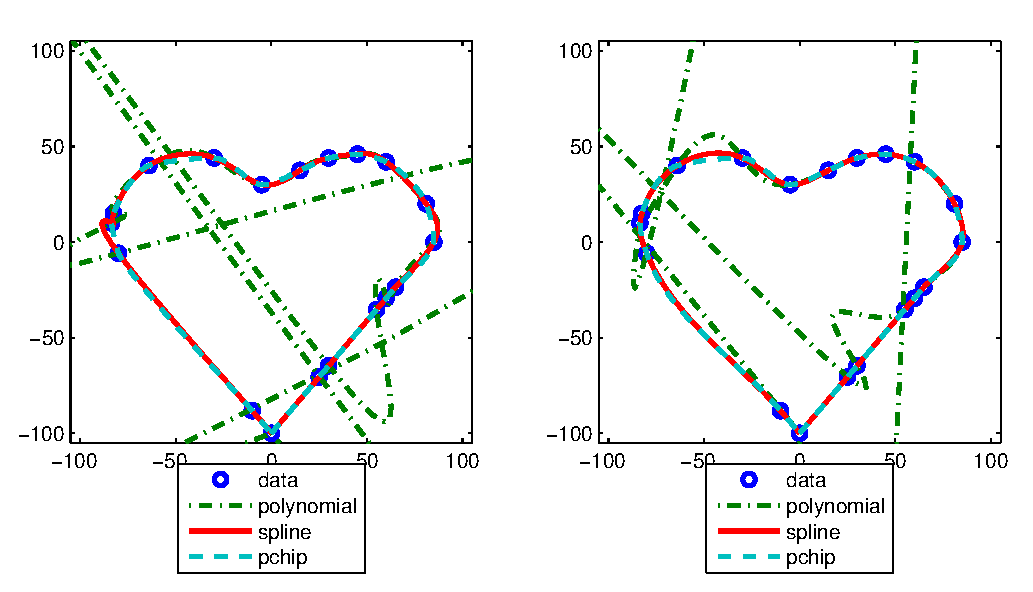
\includegraphics[width = 0.9\textwidth]{\problems/ch_piecewisepolynomials/PICTURES/ex_CurveIntp.eps}
\caption{Plots for different parametrizations and interpolation schemes}
\label{fig:ex_CurveIntp}
\end{center}\end{figure}

\textbf{Remarks:}
\begin{itemize}
 \item Note that \texttt{pchip} is a non-linear interpolation, so there is no linear mapping (matrix) from the nodes to the polynomial coefficients.
 \item Global polynomial interpolation fails. The degree of the polynomial is too high ($n$), and the typical oscillations can be observed.
 \item In this case, when two nodes are too close, spline interpolation with equidistant pa\-ra\-me\-tri\-za\-tion introduces small spurious oscillations.
\end{itemize}
\end{solution}
\end{subproblem}
\iffalse
% ============= SUBPROBLEM 5

\subproblem \label{subprb:CurveInterp_5} \difficulty{2} \pts{2}
The three interpolation schemes introduced in
subproblems~\ref{subprb:CurveInterp_1}, \ref{subprb:CurveInterp_3}, and 
\ref{subprb:CurveInterp_4} combined with either of the choices \eqref{eq:pte} and
\eqref{eq:ptl} of interpolation nodes in the parameter domain define a 
\emph{curve interpolation operator}
\begin{gather*}
  I_{\mathrm{curve}}:(\bbR^{2})^{n+1} \to \{\gamma:[0,1] \to \bbR^{2}\}\;.
\end{gather*}
Which of the six curve interpolation operators (three different interpolation
methods $\times$ two options for choosing the nodes) is linear.

\begin{solution}
Independently of the parametrization type, global polynomial and spline interpolations are linear, whereas cubic Hermite is non-linear.
}

\subproblem \label{subprb:CurveInterp_6} \difficulty{3} \pts{3}
It is interesting to study, how a transformation of the points affects the
interpolating curve:

Every linear mapping $T_A:x \mapsto \VA x$ with regular matrix $\VA \in \IR^{2,2}$
maps the plane to itself. 
%
Check experimentally whether
%
\begin{equation*}
I_{\text{curve}} ( \{ T_A \Vp_l \}_l ) = T_A I_{\text{curve}} ( \{ \Vp_l \}_l )
\end{equation*}
%
for two different matrices $A \in \{\VA_1, \VA_2\}$, given by
%
\begin{equation*}
\VA_1 =
\begin{pmatrix}
\cos(\theta) & \sin(\theta) \\
-\sin(\theta) & \cos(\theta)
\end{pmatrix}
\quad \text{with} \quad \theta = \frac{\pi}{3},
\quad \text{and} \quad
\VA_2 =
\begin{pmatrix}
1 & \lambda \\
0 & 1
\end{pmatrix}
\quad \text{with} \quad \lambda = 3, 
\end{equation*}
%
where $I_{\text{curve}} \in \{ 6 \text{ different interpolation schemes from the
  previous sub-problems} \}$. $\VA_1$ is a rotation matrix and $\VA_2$ is a shear
deformation matrix. Which matrix is orthogonal?

\begin{solution}
The code for checking whether interpolations are invariant under given linear transformations of the heart:
%
\lstinputlisting[caption={Matlab Code for \texttt{heart\_transform}},label={mc:heart_transform}]
{\problems/ch_piecewisepolynomials/MATLAB/heart_transform.m}
%
The output of \texttt{heart\_transform} is given below.
Since \texttt{pchip} is a non-linear interpolation,
it does \emph{not} commute with the linear transformation operators $A_1, A_2$.
Also, since transformation $A_2$ does not preserve distances,
the interpolation using the segment length parametrization also does not commute with $A_2$.
\\
\texttt{
\% === Errors for equidistant parametrization:\\
Error |pol\_A\_1 - A\_1\_pol| = 0.000000\\
Error |spl\_A\_1 - A\_1\_spl| = 0.000000\\
Error |pch\_A\_1 - A\_1\_pch| = 9.635142\\
Error |pol\_A\_2 - A\_2\_pol| = 0.000000\\
Error |spl\_A\_2 - A\_2\_spl| = 0.000000\\
Error |pch\_A\_2 - A\_2\_pch| = 18.519847\\
\% === Errors for segment length parametrization:\\
Error |pol\_A\_1 - A\_1\_pol| = 0.000000\\
Error |spl\_A\_1 - A\_1\_spl| = 0.000000\\
Error |pch\_A\_1 - A\_1\_pch| = 12.135839\\
Error |pol\_A\_2 - A\_2\_pol| = 252999187.352985\\
Error |spl\_A\_2 - A\_2\_spl| = 868.028069\\
Error |pch\_A\_2 - A\_2\_pch| = 865.680718\\
}\\
\fi
\end{problem}

\begin{problem}[Approximation of $\pi$]
In \lref{subsec:extrapolation} we learned about the use of polynomial extrapolation
(= interpolation outside the interval covered by the nodes) to compute
inaccessible limits $\lim\nolimits_{h\to 0}\Psi(h)$. In this problem we apply
extrapolation to obtain the limit of a sequence $x^{(n)}$ for $n\to\infty$.

We consider a quantity of interest that is defined as a limit
  \begin{gather}
    \label{eq:1}
    x^{\ast} = \lim\limits_{n\to\infty} T(n)\;,
  \end{gather}
  with a function $T:\{n,n+1,\ldots\}\mapsto\bbR$. However, computing $T(n)$ for
  very large arguments $k$ may not yield reliable results.

  The idea of \emph{extrapolation} is, firstly, to compute a few values
  $T(n_{0}),T(n_{1}),\ldots,T(n_{k})$, $k\in\bbN$, and to consider them as the values 
  $g(1/n_{0}),g(1/n_{1}),\ldots,g(1/n_{k})$ of a continuous function
  $g:]0,1/n_{\min}]\mapsto\bbR$, for which, obviously
  \begin{gather}
    \label{eq:2}
    x^{\ast} = \lim\limits_{h\to 0} g(h)\;.
  \end{gather}
  Thus we recover the usual setting for the application of polynomial
  extrapolation techniques. Secondly, according to the idea of extrapolation to
  zero, the function $g$ is approximated by an interpolating polynomial
  $p\in\Cp_{k-1}$ with $p_{k-1}(n_{j}^{-1}) = T(n_{j})$, $j=1,\ldots,k$. In many
  cases % (see \ncsesect{subsec:extrapolation} for detailed information and the
  % connection with asymptotic expansions)
  we can expect that $p_{k-1}(0)$ will
  provide a good approximation for $x^{\ast}$.  In this problem we study the
  algorithmic realization of this extrapolation idea for a simple example.

  The unit circle can be approximated by inscribed regular polygons with $n$ edges.
  The length of half of the circumference of such an $n$-edged polygon
  can be calculated by elementary geometry:
   
    \[
    \begin{array}{c|ccccccc}
      n & 2 & 3 & 4 & 5 & 6 & 8 & 10 \\
      \hline
        &  &  &  &  &  &  &  \\[-\smallskipamount]
      T(n) := \frac{U_n}{2} &\; 2 &\; \frac{3}{2}\sqrt{3} &\; 2 \sqrt{2} &\;
                                                                           \frac{5}{4}\sqrt{10-2\sqrt{5}} &\; 3 &\; 4\sqrt{2-\sqrt{2}} &\;
                                                                                                                                         \frac{5}{2} \left ( \sqrt{5}-1 \right )
    \end{array}
    \]

Write a \Cpp{} function
\begin{center}
  \texttt{double pi\_approx(int k);}
\end{center}
that uses the \emph{Aitken-Neville scheme}, see \ncseref{AitkenNeville}, to
approximate $\pi$ by extrapolation from the data in the above table, using
the first $k$ values, $k=1,\ldots,7$.


\cprotEnv \begin{solution}
 See \verb|pi_approx.cpp|.
\end{solution}


% \bigskip
%  
% We want to approximate $pi$ as half of the circumference of the unit
% circle. The circumference of the unit circle is approximated by the
% circumference of polygons fitted into the unit circle. These are given
% by geometry. Thus, we obtain the function $U(n)$, which gives us the
% circumference of the polygon with $n$ edges. We then have the
% relation, that
% \begin{equation*}
%   \lim_{n\to \infty} \frac{U(n)}{2} = \pi\ .
% \end{equation*}
% The idea is, to use interpolation, to approximate $\pi$. But for the
% function $U(n)$, we would have to evaluate the interpolation
% polynomial at $\infty$. Thus, we reformulate the problem by defining a
% function $\widetilde{U}(\frac{1}{n}) = U(n)$. Now we have
% \begin{equation*}
%   \lim_{n\to \infty} \frac{U(n)}{2} 
%   = \lim_{\frac{1}{n}\to 0} \frac{\widetilde{U}(\frac{1}{n})}{2} 
%   = \pi\ ,
% \end{equation*}
% thus, we have to interpolate $\widetilde{U}$ at zero, which is more
% reasonable than interpolating at $\infty$. Since we only need to
% interpolate at one specific point, we can use the Aitken-Neville
% scheme. This is done in \texttt{pi\_approx}.
% 
% % \lstinputlisting[caption={Matlab Code for
% %   \texttt{pi\_approx}},label={lst:pi_approx}]{pi_approx.m}
% 
% Here, we first build up the data given in the table. Then, we do a
% vectorized version of the Aitken-Neville scheme.
% 
% In the script \texttt{a1.m}, we plot the unit circle and the first few
% polygons, then approximate $\pi$ with a polynomial of degree 1 to 7,
% print out the approximation and plot the error.
% % 
% % \lstinputlisting[caption={Matlab Code for
% %   Problem 1.},label={lst:a1}]{a1.m}
% 
% The output is given below.
% 
% \begin{verbatim}
%    >> a1
%    Degree = 1, pi ~ 2.000000
%    Degree = 2, pi ~ 3.794229
%    Degree = 3, pi ~ 3.244731
%    Degree = 4, pi ~ 3.125325
%    Degree = 5, pi ~ 3.140488
%    Degree = 6, pi ~ 3.141676
%    Degree = 7, pi ~ 3.141595
% \end{verbatim}

% \begin{center}
%   \includegraphics[width=\textwidth]{a1}
% \end{center}

% We also used the function \texttt{plot\_circle}.

% \lstinputlisting[caption={Matlab Code for
%   \texttt{plot\_circle}.},label={lst:plot_circle}]{plot_circle.m}
 
\end{problem}

\end{sheet}

%%% PS8
\begin{sheet}{8}{05.11.2015}{12.11.2015}
% ncse_new/\problems/ch_piecewisepolynomials/ex_CubicSplines.tex
%  solution:  ex_CubicSpline.m  ex_CubicSpline.eps

\begin{problem}[Natural cubic Splines \coreproblem] \label{prb:NatCubicSplines}
  In \lref{sec:csi} we learned about cubic spline interpolation and its variants,
  the complete, periodic, and natural cubic spline interpolation schemes. 
  
  \begin{subproblem}[1]
    \label{csi:sp1}
    Given a knot set {$\Ct=\{t_{0}<t_{1}<\dots<t_{n}\}$}, which also serves
    as the set of interpolation nodes, and values {$y_{j}$},
    {$j=0,\ldots,n$}, write down the linear system of equations that yields
    the slopes $s'(t_{j})$ of the natural cubic spline interpolant $s$ of the data
    points $(t_{j},y_{j})$ at the knots.
    
  \begin{solution}
   Let $h_i := t_i - t_{i-1}$. Given the natural condition on the spline, one can remove the columns relative to $c_0 := s'(t_0)$ and $c_n := s'(t_n)$ from the system matrix, which becomes:
   \newcommand{\squarelineheight}{0.9ex}
   \begin{align}
    \vec{A} & := \begin{pmatrix}
                2 / h_1 & 1 / h_1 & 0 & 0 & \cdots & & 0 \\[\squarelineheight]
                b_0 & a_1 & b_1 & 0 & \cdots & & 0 \\[\squarelineheight]
                0 & b_1 & a_2 & b_2 & \ddots & & 0 \\[\squarelineheight]
                \vdots & & \ddots & \ddots & \ddots & & \vdots \\[\squarelineheight]
                \vdots & &  & b_{n-3} & a_{n-2} & b_{n-2} & 0 \\[\squarelineheight]
                0 & & \cdots & 0 & b_{n-2} & a_{n-1} & b_{n-1} \\[\squarelineheight]
                0 & & \cdots & \cdots & 0 & 1 / h_n & 2 / h_n \\
               \end{pmatrix}, a_i := \frac{2}{h_i} + \frac{2}{h_{i+1}}, b_i := \frac{1}{h_{i+1}} \\
    \vec{c} & := [ c_0, c_1, \dots, c_{n} ] \\
    \vec{b} & := [ r_0, \dots, r_{n} ]
   \end{align}
  Where $c_i := s'(t_i)$. We define $r_i := 3 \left( \frac{y_{i} - y_{i-1}}{h_{i}^2} + \frac{y_{i+1} - y_{i}}{h_{i+1}^2} \right), i = 1, \dots, n-1$, and
  \begin{align*}
   r_0 = 3 \frac{y_1 - y_0}{h_1^2}, r_n = 3 \frac{y_n - y_{n-1}}{h_n^2}
  \end{align*}
  The system becomes $\vec{A}\vec{c} = \vec{b}$.
  \end{solution}
  \end{subproblem}
  


  \begin{subproblem}[3]
    \label{csi:sp2}
    Argue why the linear system found in \autoref{csi:sp1} has a unique solution.
    
    \begin{hint}
    Look up \lref{lem:ddomspd} and apply its assertion.
    \end{hint}
    
  \begin{solution}
    Notice that $a_i := \frac{2}{h_i} + \frac{2}{h_{i+1}} > \frac{1}{h_{i+1}} + \frac{1}{h_{i}} =: b_i + b_{i-1}$. The matrix is (strictly) diagonally dominant and, therefore, invertible.
  \end{solution}
  \end{subproblem}

  \begin{subproblem}[3]
  Based on \Eigen{} devise an \emph{efficient} implementation of a \Cpp{} class for the 
  computation of a natural cubic spline interpolant with the following definition:
  \begin{lstlisting}[language=c++]
class NatCSI {
public:
    //! \brief Build the cubic spline interpolant with natural boundaries
    //! Setup the data structures you need.
    //! Pre-compute the coefficients of the spline (solve system)
    //! \param[in] t, nodes of the grid (for pairs (t_i, y_i)) (sorted!)
    //! \param[in] y, values y_i at t_i (for pairs (t_i, y_i))
    NatCSI(const const std::vector<double> & t, const const std::vector<double> & y);
    
    //! \brief Interpolant evaluation at x
    //! \param[in] x, value x where to evaluate the spline
    //! \return value of the spline at x
    double operator() (double x) const;
    
private:
    // TODO: store data for the spline
};
\end{lstlisting}
\begin{hint}
Assume that the input array of knots is sorted 
and perform binary searches for the evaluation of the interpolant.
\end{hint}
\end{subproblem}

\cprotEnv \begin{solution}
 See \verb|natcsi.cpp|.
\end{solution}
\end{problem}





\begin{problem}[Monotonicity preserving interpolation \coreproblem]
This problem is about monotonicity preserving interpolation. Before starting, you should revise \lref{def:linip}, \lref{par:datshp} and \lref{sec:hipshp} carefully.
\begin{subproblem}[4] 
Prove \lref{thm:monlinip}:

\fbox{\parbox{0.95\textwidth}{
If, for fixed node set {$\{t_{j}\}_{j=0}^{n}$}, {$n\geq2$}, an
interpolation scheme {$\Op{I}:\bbR^{n+1}\to C^{1}(I)$} is
\com{\emph{linear}} as a mapping from data values to continuous functions on
the interval covered by the nodes ($\to$ \lref{def:linip}), and
\com{\emph{monotonicity preserving}}, then \com{$\Op{I}(\Vy)'(t_{j})=0$} for
all {$\Vy\in\bbR^{n+1}$} and {$j=1,\ldots,n-1$}.}}

\begin{hint}
Consider a suitable basis $\{\mathbf{s}^{(j)}:j=0,\dots,n\}$ of $\R^{n+1}$ that consists of monotonic vectors, namely such that $s^{(j)}_i \le s^{(j)}_{i+1}$ for every $i=0,\dots,n-1$.
\end{hint}
\begin{hint}
Exploit the phenomenon explained next to \lref{monintp}.
\end{hint}
\begin{solution}
Without loss of generality assume that $t_0 < t_1 < \dots <t_n$. For $j=0,\dots,n$ let $\mathbf{s}^{(j)}\in\R^{n+1}$ be defined by
\[
s^{(j)}_i=
\begin{cases}
0 & i=0,\dots,j-1 \\
1 & i=j,\dots,n.
\end{cases}
\]
Clearly, $(t_i,s^{(j)}_i)_i$ are monotonic increasing data, according to \lref{def:mondata}.

%In particular, $\mathbf{s}^{(0)}=(1,\dots,,1)^T$ is the constant vector, hence it is monotonic increasing and decreasing. Since $\Op{I}$ is monotonicity preserving, this implies that $\Op{I}(\mathbf{s}^{(0)})$ is both increasing and decreasing, and so it is constant. As a consequence, its derivative is constantly zero. In particular,
%\begin{equation}
%label{eq:s0}
%(\Op{I}(\mathbf{s}^{(0)}))'(t_i)=0,\quad i=1,\dots,n-1.
%\end{equation}

Take $j=0,\dots,n$. Note that $\mathbf{s}^{(j)}$ has a local extremum in $t_i$ for every $ i=1,\dots,n-1$. Thus, since $\Op{I}$ is monotonicity preserving (see \lref{par:shppres}),
 $\Op{I}(\mathbf{s}^{(j)})$ has to be flat in $t_i$ for every $ i=1,\dots,n-1$ (see \lref{sec:hipshp}). As a consequence,
\begin{equation}
\label{eq:sj}
(\Op{I}(\mathbf{s}^{(j)}))'(t_i)=0,\quad i=1,\dots,n-1.
\end{equation}

Note now that $\{\mathbf{s}^{(j)}:j=0,\dots,n\}$ is a basis for $\R^{n+1}$ (indeed, they constitute a linearly independent set with cardinality equal to the dimension of the space). As a consequence, every $\mathbf{y}\in\R^{n+1}$ can be written as a linear combination of the $\mathbf{s}^{(j)}$s, namely
\[
\mathbf{y}=\sum_{j=0}^n \alpha_j \mathbf{s}^{(j)}.
\]
Therefore, by the linearity of $\Op{I}$ and using \eqref{eq:sj}, for every $i=1,\dots,n-1$ we obtain
\[
(\Op{I}(\mathbf{y}))'(t_i)=\left(\Op{I}\left(\sum_{j=0}^n \alpha_j \mathbf{s}^{(j)}\right)\right)'(t_i) 
=\left(\sum_{j=0}^n \alpha_j \Op{I}(\mathbf{s}^{(j)})\right)'(t_i) 
=\sum_{j=0}^n \alpha_j \Op{I}(\mathbf{s}^{(j)})'(t_i) 
=0,
\]
as desired.
\end{solution}
\end{subproblem}
\end{problem}

\begin{problem}[Local error estimate for cubic Hermite interpolation \coreproblem]
 
 Consider the cubic Hermite interpolation operator $\mathcal{H}$ of a function defined on an interval $[a,b]$ to the space  $\mathcal{P}_3$ polynomials of degree at most $3$:
 \[
  \mathcal{H}: C^1([a,b]) \rightarrow \mathcal{P}_3
 \]
defined by:
\begin{itemize}
 \item $(\mathcal{H}f)(a) = f(a)$;
 \item $(\mathcal{H}f)(b) = f(b)$;
 \item $(\mathcal{H}f)'(a) = f'(a)$;
 \item $(\mathcal{H}f)'(b) = f'(b)$.
\end{itemize}
Assume $f \in C^4([a,b])$. Show that for every $x \in ]a,b[$ there exists $\tau \in [a,b]$ such that\begin{align}
 (f - \mathcal{H}f)(x) = \frac{1}{24} f^{(4)}(\tau) (x - a)^2(x-b)^2.
\end{align}

\begin{hint}
 Fix $x \in ]a,b[$. Use an auxiliary function:
 \begin{align}
  \varphi(t) := f(t) - (\mathcal{H}f)(t) - C (t-a)^2(t-b)^2.
 \end{align}
 Find $C$ s.t. $\varphi(x) = 0$.
\end{hint}

\begin{hint}
 Use Rolle's theorem (together with the previous hint and the definition of $\mathcal{H}$) to find a lower bound for the number of zeros of $\varphi^{(k)}$ for $k = 1,2,3,4$.
\end{hint}

\begin{hint}
 Use the fact that $(\mathcal{H}f) \in \mathcal{P}_3$ and for $p(t) := (t - a)^2(t - b)^2, p \in \mathcal{P}_4$.
\end{hint}


\begin{hint}
 Conclude showing that $\exists \tau \in ]a,b[, \varphi^{(4)}(\tau) = 0$. Use the definition of $\varphi$ to find an expression for $C$.
\end{hint}


\begin{solution}
 Fix $x \in ]a,b[$. Define:
 \begin{align}
  \varphi(t) := f(t) - \mathcal{H}f(t) - C (t-a)^2(t-b)^2
 \end{align}
 with
 \[
C := \frac{f(x) - \mathcal{H}f(x)}{(x-a)^2(x-b)^2}.
 \]
 Then $\varphi(a) = \varphi(b) = \varphi'(a) = \varphi'(b) = 0$ (using the definition of $\mathcal{H}$). Moreover $\varphi(x) = 0$ (by construction). Therefore, by Rolle's theorem ($\varphi$ has at least two local extrema), $\exists \xi_1, \xi_2 \in ]a,b[, \xi_1 \neq \xi_2$ such that $\varphi'(\xi_1) = \varphi'(\xi_2) = 0$. \\
 $\Rightarrow \varphi'$ has at least 4 zeros in $[a,b]$ ($a, b, \xi_1$ and $\xi_2$ are pairwise distinct). \\
 $\Rightarrow \varphi''$ has at least 3 zeros in $[a,b]$ ($\varphi'$ has at least 3 local extrema). \\
 $\Rightarrow \varphi^{(3)}$ has at least 2 zeros in $[a,b]$ ($\varphi''$ has at least 2 local extrema). \\
 $\Rightarrow \varphi^{(4)}$ has at least 1 zero in $[a,b]$ ($\varphi^{(3)}$ has at least one local extrema), let $\tau$ be such zero. \\
 $\Rightarrow 0 = \varphi^{(4)}(\tau) = f^{(4)}(\tau) - 24 C$. \\
 $\Rightarrow C = \frac{1}{24} f^{(4)}(\tau)$. $\qed$
\end{solution}

\end{problem}

% ncse_new/p2_InterpolationApproximation/ch1_PolynomialInterpolation/ex_ChebIntp2.tex
% exercise requires:    -
% solutions require:    adaptivepolyintp.m  plot_adaptivepolyintp.m  plot_adaptivepolyintp.eps


\begin{problem}[Adaptive polynomial interpolation]\label{prb:ChebIntp2}

In \ncsesect{sec:ChebychevInterpolation} we have seen that the placement of
interpolation nodes is key to a good approximation by a polynomial
interpolant. The following \emph{greedy algorithm} attempts to find the location
of suitable nodes by its own:
\begin{quote}
  Given a function $f:[a,b]\mapsto \bbR$ one starts
  $\Ct:=\{\frac{1}{2}(b+a)\}$. Based on a fixed finite set
  $\Cs\subset[a,b]$ of \emph{sampling points} one augments the set of nodes
  according to
  \begin{gather}
    \label{rb:1}
    \Ct = \Ct \cup \left\{\operatorname*{argmax}\limits_{t\in\Cs}
    |f(t)-\Op{I}_{\Ct}(t)|\right\}\;,
  \end{gather}
  where $\Op{I}_{\Ct}$ is the polynomial interpolation operator for
  the node set $\Ct$, until 
  \begin{gather}
    \label{rb:2}
    \operatorname*{max}\limits_{t\in\Cs}
   |f(t)-\Op{I}_{\Ct}(t)| \leq \mathtt{tol}\cdot 
   \operatorname*{max}\limits_{t\in\Cs}
    |f(t)|\;.
  \end{gather}
\end{quote}

% ============== SUBPROBLEM 1

\begin{subproblem}[3]\label{subprb:ChebIntp2_1}
Write a MATLAB function 
\begin{center}
  \texttt{function t = adaptivepolyintp(f,a,b,tol,N)}
\end{center}
that implements the algorithm described above and takes as arguments the function
handle \texttt{f}, the interval bounds \texttt{a}, \texttt{b}, the
relative tolerance \texttt{tol}, and the number \texttt{N} of 
\emph{equidistant} sampling points (in the interval $[a,b]$), that is,
\begin{gather*}
  \Cs := \{a+(b-a)\frac{j}{N},\;j=0,\ldots,N\}\;.
\end{gather*}

\begin{hint}
The function \texttt{intpolyval} from \ncseref[Code]{barycentricformula}
is provided and may be used (though it may not be the most efficient way
to implement the function).
\end{hint}

\begin{solution}
See \autoref{mc:ChebIntp2_adaptivepolyintp}.
\end{solution}
\end{subproblem}

% ============== SUBPROBLEM 2

\begin{subproblem}[2]\label{subprb:ChebIntp2_2}
Extend the function from the previous sub-problem so that it
reports the quantity 
\begin{gather}
\label{AIP:1}
\operatorname*{max}\limits_{t\in\Cs}
|f(t)-\Op{T}_{\Ct}(t)| % \leq \mathtt{tol}
\end{gather}
for each intermediate set $\Ct$. 

\begin{solution}
See \autoref{mc:ChebIntp2_adaptivepolyintp}.
%
\lstinputlisting[caption={Implementation of the function \texttt{adaptivepolyintp}},label={mc:ChebIntp2_adaptivepolyintp}]
{\problems/ch_polynomialinterpolation/MATLAB/adaptivepolyintp.m}
\end{solution}
\end{subproblem}

% ============== SUBPROBLEM 3

\begin{subproblem}[2]\label{subprb:ChebIntp2_3} 
For $f_{1}(t) :=
\sin(e^{2t})$ and $f_{2}(t) = \frac{\sqrt{t}}{1+16t^{2}}$ plot the quantity from
\eqref{AIP:1} versus the number of interpolation nodes. Choose plotting styles
that reveal the qualitative decay of this error as the number of interpolation
nodes is increased. Use interval $[a,b] = [0,1]$, \texttt{N=1000} sampling points,
tolerance \texttt{tol = 1e-6}.

\begin{solution}
See \autoref{mc:ChebIntp2_plot_adaptivepolyintp} and \autoref{fig:ChebIntp2_plot_adaptivepolyintp}.
%
\lstinputlisting[caption={Implementation of the function \texttt{plot\_adaptivepolyintp}},label={mc:ChebIntp2_plot_adaptivepolyintp}]
{\problems/ch_polynomialinterpolation/MATLAB/plot_adaptivepolyintp.m}
%
\begin{figure}
\centering
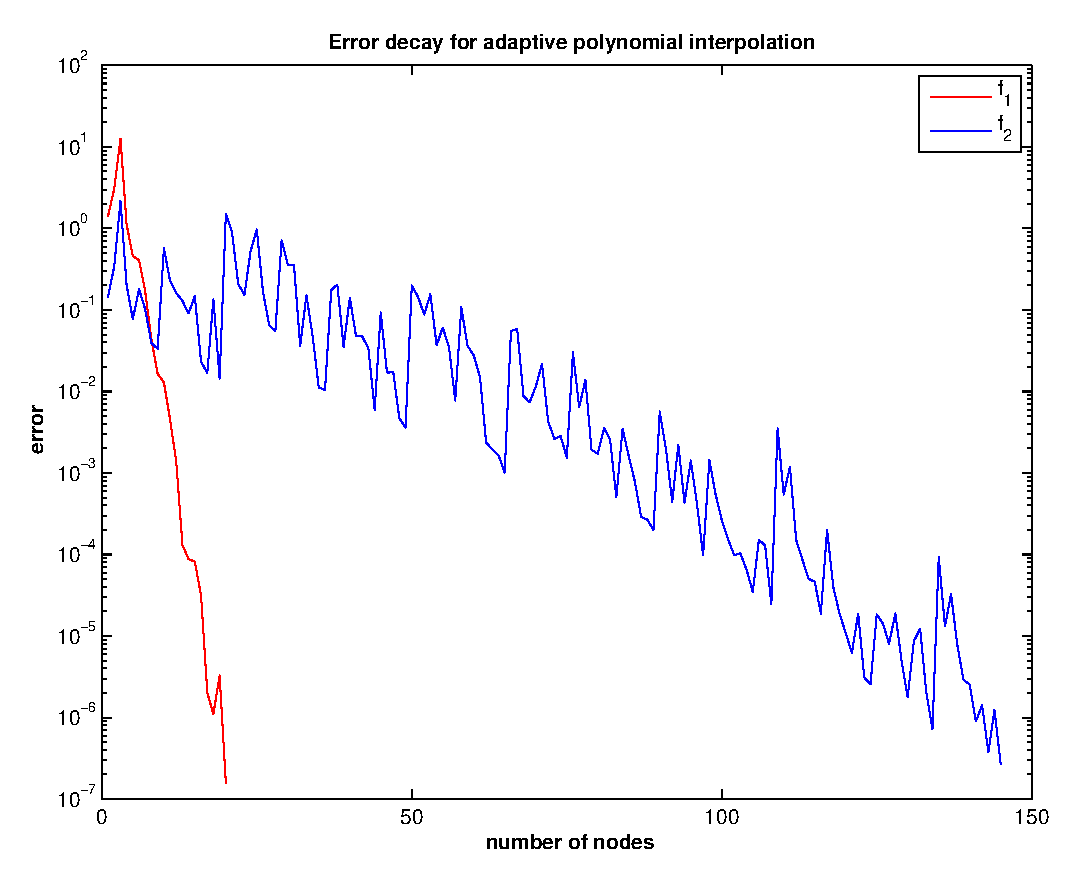
\includegraphics[width=0.7\textwidth]{\problems/ch_polynomialinterpolation/PICTURES/plot_adaptivepolyintp.eps}
\caption{The quantity from \eqref{AIP:1}
versus the number of interpolation nodes.}
\label{fig:ChebIntp2_plot_adaptivepolyintp}
\end{figure}
\end{solution}
\end{subproblem}
\end{problem}

\end{sheet}

%%% PS9
\begin{sheet}{9}{12.11.2015}{19.11.2015}\label{PS9}
\begin{problem}[Chebychev interpolation of analytic functions \coreproblem] 
 
This problem concerns Chebychev interpolation
(cf. \ncsesect{sec:ChebychevInterpolation}). Using techniques from complex
analysis, notably the residue theorem \lref{thm:residue}, in class we derived an
expression for the interpolation error \lref{eq:recipform} and from it an error
bound \lref{eq:intperrbd}, as much sharper alternative to \ncseref{cor:polintperr}
and \ncseref{thm:polintperr} for \emph{analytic} interpolands. The bound tells us
that for all $t\in [a,b]$
\begin{align*}
  \lvert f(t) - \Op{L}_{\Ct} f(t) \rvert 
   \leq 
   \left\lvert \frac{w(x)}{2 \pi i} \int_\gamma 
   \frac{f(z)}{(z-t) w(z)} dz \right\rvert 
  \leq \frac{\lvert \gamma \rvert}{2 \pi} 
  \frac{\max_{a \leq \tau \leq b}\lvert w(\tau) \rvert}{\min_{z \in  \gamma}\lvert
  w(z) \rvert} 
  \frac{ \max_{z \in \gamma} \lvert f(z) \rvert }{d([a,b], \gamma)}\;,
\end{align*}
where {$d([a,b],\gamma)$} is the geometric distance of the integration contour
$\gamma\subset\bbC$ from the interval $[a,b]\subset\bbC$ in the complex plane. The
contour $\gamma$ must be contractible in the domain $D$ of analyticity of $f$ and
must wind around $[a,b]$ exactly once, see \lref{analintp}. 

Now we consider the interval $[-1,1]$. Following \ncserem{rem:chebipanal}, our
task is to find an upper bound for this expression, in the case where $f$
possesses an analytical extension to a complex neighbourhood of $[-1,1]$.

For the analysis of the Chebychev interpolation of analytic functions we used the
elliptical contours, see \lref{ellipses},
\begin{align}
 \gamma_\rho(\theta) := \cos(\theta - i \log(\rho) )\;,\quad
  \forall 0 \leq \theta \leq 2 \pi\;,\quad \rho > 1\;.
\end{align}

\begin{subproblem}[2]
 Find an upper bound for the length $\lvert \gamma_\rho \rvert$ of the contour $\gamma_\rho$.
 
 \begin{hint}
  You may use the arc-length formula for a curve $\gamma: I \rightarrow \IR^2$:
  \begin{align}
   \lvert \gamma \rvert = \int_I \lVert \dot\gamma(\tau) \rVert d\tau,
  \end{align}
  where $\dot\gamma$ is the derivative of $\gamma$ w.r.t the parameter
  $\tau$. Recall that the ``length'' of a complex number $z$ viewed as a vector in 
  $\bbR^{2}$ is just its modulus. 
 \end{hint}

 \begin{solution}
  $\frac{\partial \gamma_\rho(\theta)}{\partial \theta} := -\sin(\theta - i \log(\rho) )$, therefore:
  \begin{align}
   \lvert \gamma_\rho \rvert & = \int_{[0,2 \pi]} \lvert \sin(\tau - i \log(\rho) ) \rvert d\tau \\
   & = \frac{1}{2 \rho} \int_{[0,2 \pi]} \sqrt{ \sin^2(\tau) (1 + \rho^2)^2 + \cos^2(\tau) (1 - \rho^2)^2 } d\tau \\
   & \leq \frac{1}{2 \rho} \int_{[0,2 \pi]} \sqrt{ 2 + 2\rho^4 } d\tau
   & \leq \frac{1}{\rho} \pi \sqrt{ 2 (1 + \rho^4) }
  \end{align}
 \end{solution}
\end{subproblem}

Now consider the $S$-curve function (the logistic function):
\begin{align*}
 f(t) := \frac{1}{1+e^{-3t}}\;,\quad t \in \IR\;.
\end{align*}

\begin{subproblem}[2] \label{subprb:max_dom_analyticity}
 Determine the maximal domain of analyticity of the extension of $f$ to the complex plane $\IC$.
 \begin{hint}
  Consult \lref{rem:analfunc}.
 \end{hint}
 
 \begin{solution}
  $f$ is analytic in $D := \IC \setminus \{ \frac{2}{3} \pi i c - \frac{1}{3} \pi i \; | \; c \in \IZ \}$. In fact, $g(t) := 1 + exp(-3t)$ is an entire function, whereas $h(x) := \frac{1}{x}$ is analytic in $\IC \setminus \{ 0 \}$. Therefore, using \ncseref{thm:analchain}, $f$ is analytic in $\IC \setminus \{ z \in \IC \; | \; g(z) = 0 \} =: \IC \setminus S$. 
  Let $z := a + ib$, $a,b \in \IR$. Since:
  \begin{align}
   -1 = \exp(z) = \exp(a + ib) = \exp(a) (\cos(b) + i \sin(b)) & \Leftrightarrow a = 0, b \in 2 \pi \IZ + \pi \\
   \exp(z) = -1 & \Leftrightarrow z \in i(2 \pi  \IZ + \pi) \\
   \exp(-3z) = -1 & \Leftrightarrow z \in \frac{i(2 \pi \IZ - \pi)}{3}
  \end{align}
  Therefore $S = \frac{2}{3} \pi i \IZ - \frac{1}{3} \pi i$.
 \end{solution}
\end{subproblem}

\begin{subproblem}[2] \label{subprb:compute_upper_bound_cheby}
 Write a \Matlab{} function that computes an approximation $M$ of:
 \begin{align}
  \min_{\rho > 1} \frac{ \max_{z \in \gamma_\rho} \lvert f(z) \rvert }{d([-1,1], \gamma_\rho)},
 \end{align}
 by sampling, where the distance of $[a,b]$ from $\gamma_{\rho}$ is formally
 defined as
 \begin{align}
  d([a,b], \gamma) := \inf \{ \lvert z - t \rvert \; | \; z \in \gamma, t \in [a,b] \}.
 \end{align}

 \begin{hint}
  The result of \ref{subprb:max_dom_analyticity}, together with the knowledge that $\gamma_\rho$ describes an ellipsis, tells you the maximal range $(1,\rho_{max})$ of $\rho$. Sample this interval with $1000$ equidistant steps.
 \end{hint}
 
 \begin{hint}
  Apply geometric reasoning to establish that the
  distance of $\gamma_\rho$ and $[-1,1]$ is $\frac{1}{2}(\rho + \rho^{-1}) - 1$.
 \end{hint}
 
 \begin{hint}
  If you cannot find $\rho_{max}$ use $\rho_{max} = 2.4$.
 \end{hint}
 
 \begin{hint}
  You can exploit the properties of $\cos$ and the hyperbolic trigonometric functions $\cosh$ and $\sinh$.
 \end{hint}

\cprotEnv \begin{solution}
  The ellipse must be restricted such that the minor axis has length $\leq 2 \pi / 3$ ($2$ times the smallest point, in absolute value, where $f$ is not-analytic). Since this corresponds to the imaginary part of $\gamma_\delta(\theta)$, when $\theta = \pi / 2$, we find:
  \begin{align*}
   \cos(\pi / 2 - i \log(\rho_{max})) = 1 / 3 \pi i \Leftrightarrow \sinh(\log(\rho_{max})) = \pi/3 \Leftrightarrow \rho_{max} = \exp(\sinh^{-1}(\pi / 3)).
  \end{align*}
  See \verb|cheby_approx.m| and \verb|cheby_analytic.m| for the \Matlab{} code.
 \end{solution}
\end{subproblem}

\begin{subproblem}[2]
  \label{cheb:sp:bd}
 Based on the result of \ref{subprb:compute_upper_bound_cheby}, and  \ncseref{eq:chebanalest}, give an ``optimal'' bound for
 \begin{align*}
  \lVert f - L_n f \rVert_{L^\infty([-1,1])},
 \end{align*}
 where $L_n$ is the operator of Chebychev interpolation on $[-1,1]$ into the space
 of polynomials of degree $\leq n$.

 \begin{solution}
 Let $M$ be the approximation of \ref{subprb:compute_upper_bound_cheby}. Then
 \begin{align*}
   \lVert f - L_n f \rVert_{L^\infty([-1,1])} \lesssim \frac{M \sqrt{2 (\rho^{-2} + \rho^{2})}}{\rho^{n+1} - 1}.
 \end{align*}
 \end{solution}
\end{subproblem}

\begin{subproblem}[1]
  Graphically compare your result from \ref{cheb:sp:bd} with the measured supremum
  norm of the approximation error of Chebychev interpolation of $f$ on $[-1,1]$
  for polynomial degree $n = 1,\dots,20$. To that end, write a \Matlab{}-code and
  rely on the provided function \verb|intpolyval| (cf. \ncseref{trigpolyval}).
 \begin{hint}
  Use semi-logarithmic scale for your plot \verb|semilogy|.
 \end{hint}
 \cprotEnv \begin{solution}
   See \verb|cheby_analytic.m|.
 \end{solution}
\end{subproblem}

\begin{subproblem}[4]
 Rely on pullback to $[-1,1]$ to discuss how the error bounds in
 \ncseref{eq:chebanalest} will change when we consider Chebychev interpolation on
 $[-a,a], a > 0$, instead of $[-1,1]$, whilst keeping the function $f$ fixed.

 \begin{solution}
   The rescaled function $\Phi^{\ast}f$ will have a different domain of
     analyticity and a different growth behavior in the complex plane. The larger
     $a$, the closer the pole of $\Phi^{\ast}f$ will move to $[-1,1]$, the more
     the choice of the ellipses is restricted (i.e. $\rho_{max}$ becomes smaller). This will result in a larger bound.
   
   Using \ncseref{eq:tpdft}, if follows immediately that the asymptotic behaviour of the interpolation does not change after rescaling of the interval. In fact, if $\Phi^*$ is the affine pullback from $[-a,a]$ to $[-1,1]$, then:
   \begin{align*}
     \lVert f - \hat{(L_n)} f \rVert_{L^\infty([-a,a])} = \lVert \Phi^* f - L_n \Phi^* f \rVert_{L^\infty([-1,1])},
   \end{align*}
   where $\hat{(L_n)}$ is the interpolation on $[-a,a]$.
 \end{solution}
 \end{subproblem}

\end{problem}

% ncse_new/\problems/ch_piecewisepolynomials/ex_GradedMeshes.tex
% exercise requires:   GradedMesh.eps
% solutions require:   PWlineConv.m  PWlineIntp.m  PWlineConv.eps  GradedMesh.m  PWlineGraded.m  PWlineGraded_0.50.eps

\begin{problem}[Piecewise linear approximation on graded meshes \coreproblem]
  \label{prb:GradedMeshes}

One of the messages given by \lref{sec:ChebychevInterpolation}
is that the quality of an interpolant depends heavily on the choice of the
interpolation nodes.  If the function to be interpolated has a ``bad behavior'' in
a small part of the domain, for instance it has very large derivatives of high
order, more interpolation points are required in that area of the domain.
Commonly used tools to cope with this task, are \textit{graded meshes}, which
will be the topic of this problem.

\vspace{4mm}

Given a mesh $\Ct=\{0\le t_0<t_1<\cdots<t_n\le1\}$ on the unit interval $I=[0,1]$, $n\in\IN$, we define the \textit{piecewise linear} interpolant
$$\Isf_\Ct:C^0(I)\rightarrow \Cp_{1,\Ct} = \{ s\in C^0(I),\; s_{|[t_{j-1},t_j]}\in\Cp_1\;\forall\;j \},
\quad\text{s.t.}\quad \big(\Isf_\Ct f\big) (t_j)=f(t_j),\quad j=0,\ldots,n; $$
(see also \lref{sec:piecewise-linear-interp}).


\begin{subproblem}[2]
\label{subprb:GradedMeshes_1}
If we choose the uniform mesh $\Ct=\{t_j\}_{j=0}^n$ with $t_j=j/n$, given a function $f\in C^2(I)$, what is the asymptotic behavior of the error
$$\N{f-\Isf_\Ct f}_{L^\infty(I)},$$
when $n\rightarrow\infty$?

\begin{hint}
Look for a suitable estimate in \lref{sec:ppi}.
\end{hint}

\begin{solution}
Equation \ncseeq{pwintp:LinfConv} says
$$\N{f-\Isf_\Ct f}_{L^\infty(I)}  \leq \frac1{2n^2}\N{f^{(2)}}_{L^\infty(I)}, $$
because the meshwidth is $h=1/n$. So, the convergence is quadratic, i.e., algebraic with order 2.
\end{solution}
\end{subproblem}



%%%%%%%%%%%%%%%%%%%%%%%%%%%%%%%%%%%%%%%%%%%%%%%%%%%%%%%%%%%

\begin{subproblem}[2]\label{subprb:GradedMeshes_2}
What is the regularity of the function
$$f:I\rightarrow\IR,\qquad f(t)=t^\alpha, \qquad 0<\alpha<2\;?$$
In other words, for which $k\in\IN$ do we have $f\in C^k(I)$? 

\begin{hint}
Notice that $I$ is a closed interval and check the continuity of the derivatives in the endpoints of $I$.
\end{hint}

\begin{solution}
If $\alpha=1$, $f(t)=t$ clearly belongs to $C^\infty(I)$.
If $0<\alpha<1$, $f'(t)=\alpha t^{\alpha-1}$ blows up to infinity for $t$ going to $0$, therefore $f\in C^0(I)\setminus C^1(I)$.
If $1<\alpha<2$, $f'$ is continuous but $f''(t)=\alpha(\alpha-1) t^{\alpha-2}$ blows up to infinity for $t$ going to $0$, 
therefore $f\in C^1(I)\setminus C^2(I)$.

More generally, for $\alpha\in \IN$ we have $f(t)=t^\alpha\in C^\infty(I)$; on the other hand if $\alpha>0$ is not an integer, $f\in C^{\lfloor \alpha\rfloor}(I)$, where $\lfloor \alpha\rfloor =\mathrm{floor}(\alpha) $ is the largest integer not larger than $\alpha$.
\end{solution}
\end{subproblem}





%%%%%%%%%%%%%%%%%%%%%%%%%%%%%%%%%%%%%%%%%%%%%%%%%%%%%%%%%%%

\begin{subproblem}[3]\label{subprb:GradedMeshes_2half}
Study numerically the $h$-convergence of the piecewise linear approximation of
$f(t)=t^\alpha$ ($0<\alpha<2$) on uniform meshes; determine the order of
convergence using linear regression based on \Matlab's \texttt{polyfit}, see
\ncsesect{sec:ppi}.

\begin{hint}
Linear regression and \texttt{polyfit} have not been introduced yet. Please give a quick look at the examples in \href{http://ch.mathworks.com/help/matlab/ref/polyfit.html\#examples}{http://ch.mathworks.com/help/matlab/ref/polyfit.html\#examples} to see \texttt{polyfit} in action. For instance, the code to determine the slope of a line approximating a sequence of points $(x_i,y_i)_i$ in doubly logarithmic scale is
\begin{lstlisting}
P = polyfit(log(x),log(y),1);
slope = P(1);
\end{lstlisting}
\end{hint}

\begin{solution}The interpolant is implemented in Listing~\ref{mc:PWlineIntp}, the convergence for our choice of $f$ is studied in file \texttt{PWlineConv.m} and the results are plotted in Figure~\ref{fig:PWlineConv}.
The convergence is clearly algebraic, the rate is equal to $\alpha$ if it is smaller than 2, and equal to 2 otherwise.
In  brief, we can say that the order is $\min\{\alpha,2\}$.

Be careful with the case $\alpha=1$: here the interpolant gets exactly the solution, with every mesh.

\lstinputlisting[caption={Piecewise linear interpolation.},label={mc:PWlineIntp}]
{\problems/ch_piecewisepolynomials/MATLAB/PWlineIntp.m}


\begin{figure}[htb]
\caption{$h$-convergence of piecewise linear interpolation for $f(t)= t^\alpha$, $\alpha=0.1,0.3,\ldots,2.9$.
The convergence rates are shown in the small plot.}
\label{fig:PWlineConv}\begin{center}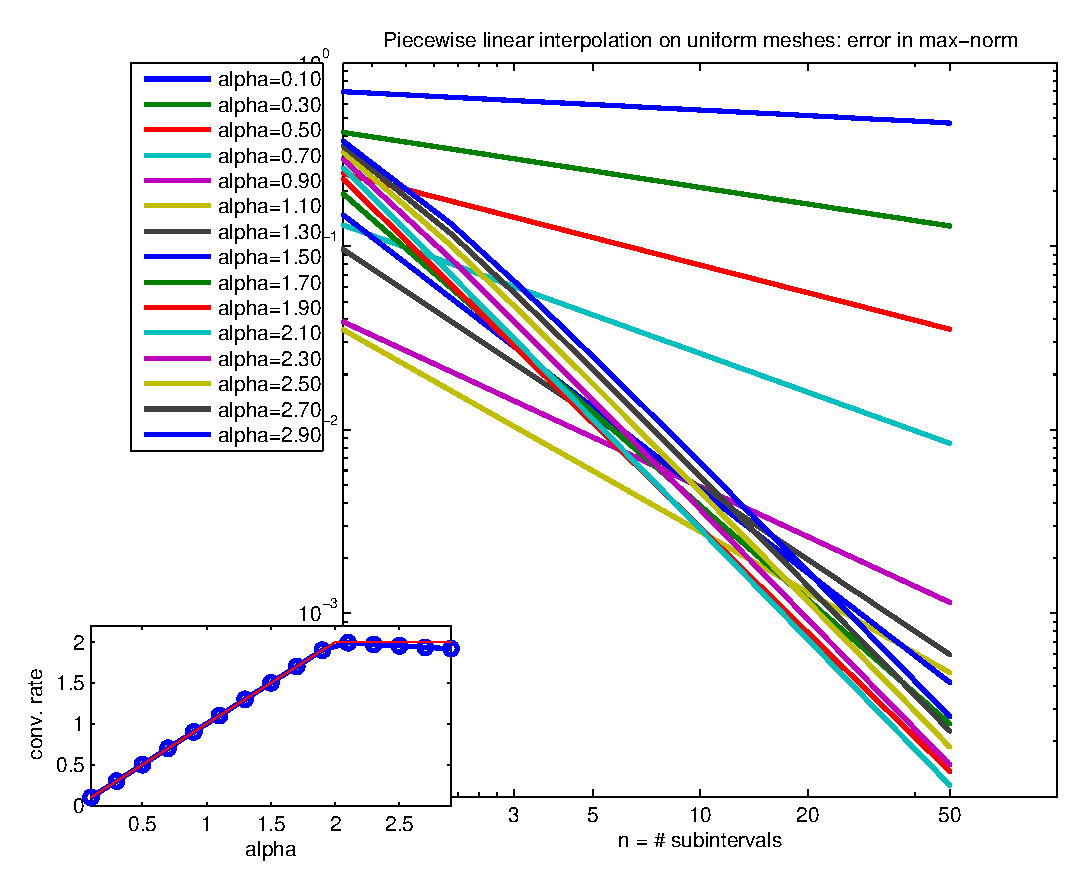
\includegraphics[width=0.85\textwidth]{\problems/ch_piecewisepolynomials/PICTURES/PWlineConv.eps}\end{center}\end{figure}
\end{solution}
\end{subproblem}





%%%%%%%%%%%%%%%%%%%%%%%%%%%%%%%%%%%%%%%%%%%%%%%%%%%%%%%%%%%

\begin{subproblem}[3]\label{subprb:GradedMeshes_3}
In which mesh interval do you expect $|f-\Isf_{\Ct}f|$ to attain its maximum?

\begin{hint}
You may use the code from the previous subtask to get an idea.
\end{hint}
\begin{hint}
What is the meaning of \ncsethm{cor:polintperr}  in the piecewise linear setting? 
\end{hint}

\begin{solution}The error representation \ncseeq{intp:thm-error-estim} in the linear case ($n=1$) reads
\begin{align*}
 \forall\;t\in(t_j,t_{j+1})\qquad  \Big|f(t)-\big(\Isf_{\Ct}f\big)(t)\Big| &=\frac12 |f''(\tau_t) \; (t-t_j)(t-t_{j+1})| \\
&\leq \frac18 |f''(\tau_t)|\; (t_{j+1}-t_{j})^2 = \frac1{8n^2}|f''(\tau_t)|,
\end{align*}
for some $\tau_t\in(t_j,t_{j+1})$.
Therefore the error can be large only in the subintervals where the second derivative of $f$ is large.
But
$$|f''(t)|=\big|\alpha(\alpha-1)t^{\alpha-2}\big|$$
is monotonically decreasing for $0<\alpha<2$, therefore we can expect a large error in the first subinterval, the one that is closer to $0$.

In line 23 of the code in \texttt{PWlineConv.m},  we check our guess: the maximal error is found in the first interval for every $\alpha\in(0,2)$ ($\alpha\ne1$) and in the last one for $\alpha>2$.
\end{solution}
\end{subproblem}




%%%%%%%%%%%%%%%%%%%%%%%%%%%%%%%%%%%%%%%%%%%%%%%%%%%%%%%%%%%

\begin{subproblem}[3]\label{subprb:GradedMeshes_4}
Compute by hand the exact value of $\N{f-\Isf_{\Ct}f}_{L^\infty(I)}$.

Compare the order of convergence obtained with the one observed numerically in \ref{subprb:GradedMeshes_2}.

\begin{hint}
Use the result of \ref{subprb:GradedMeshes_3} to simplify the problem.
\end{hint}

\begin{solution}From \ref{subprb:GradedMeshes_3} we expect that the maximum is taken in the first subinterval.
For every  $t\in(0,1/n)$ and $0<\alpha<2$ ($\alpha\ne1$) we compute the minimum of the error function $\varphi$ 
\begin{align*}
\varphi(t)   &=f(t)-\big(\Isf_{\Ct}f\big)(t) = t^\alpha- t\;\frac1{n^{\alpha-1}},\hspace{2cm}(\varphi(0)=\varphi(1/n)=0),\\
\varphi'(t)  &= \alpha t^{\alpha-1}- \frac1{n^{\alpha-1}},\\
\varphi'(t^*)&=0\quad\text{if}\quad t^* = \frac 1n\alpha^{1/(1-\alpha)} \le\frac1{2n},\\          % <=1/2   is not easy.....
\max_{t\in(0,1/n)}|\varphi(t)|&=|\varphi(t^*)|=\Big|\frac{\alpha^{\alpha/(1-\alpha)}}{n^\alpha}-\frac{\alpha^{1/(1-\alpha)}}{n^\alpha}\Big|
              =\frac1{n^\alpha}\Big|\alpha^{\alpha/(1-\alpha)}-\alpha^{1/(1-\alpha)}\Big|    = \Co(n^{-\alpha}) = \Co(h^{\alpha}).
\end{align*}
The order of convergence in $h=1/n$ is equal to the parameter $\alpha$, as observed in Figure~\ref{fig:PWlineConv}.
\end{solution}
\end{subproblem}



%%%%%%%%%%%%%%%%%%%%%%%%%%%%%%%%%%%%%%%%%%%%%%%%%%%%%%%%%%%

\begin{subproblem}[3]\label{subprb:GradedMeshes_5}
Since the interpolation error is concentrated in the left part of the domain, it seems reasonable to use a finer mesh only in this part.
A common choice is an \textbf{algebraically graded mesh}, defined as
$$\Cg=\Big\{t_j=\Big(\frac jn\Big)^\beta,\quad j=0,\ldots,n\Big\},$$
for a parameter $\beta>1$.
An example is depicted in Figure~\ref{fig:GradedMesh} for $\beta=2$.

\begin{figure}[htb]\caption{Graded mesh $x_j=(j/n)^2$, $j=0,\ldots,10$.}\label{fig:GradedMesh}
\begin{center}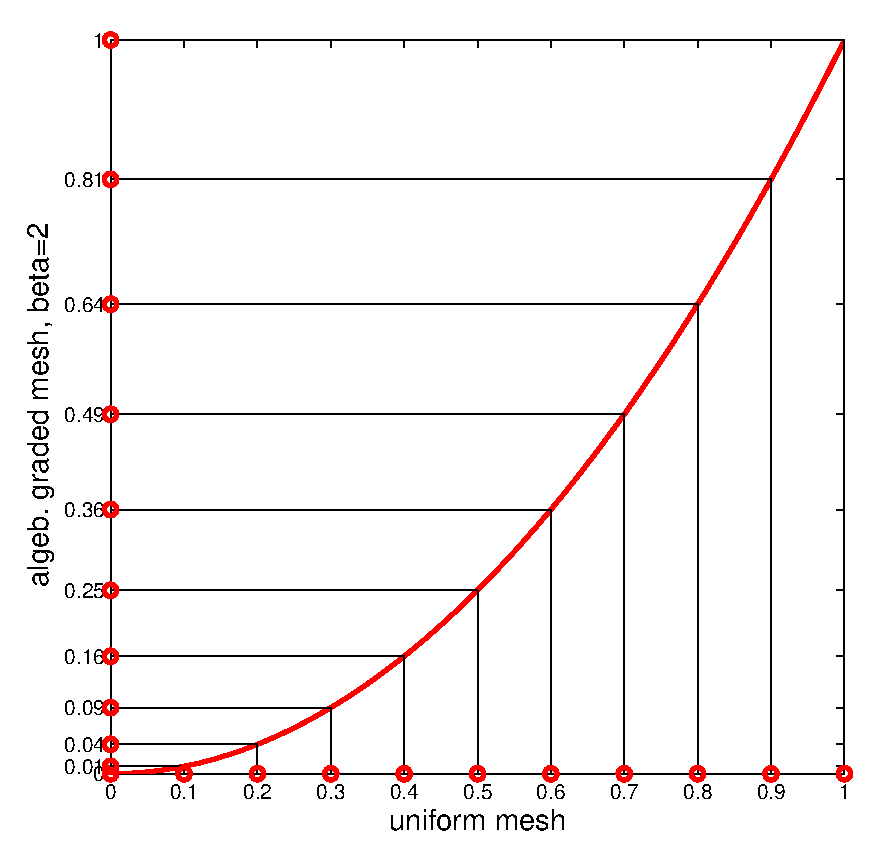
\includegraphics[width=0.5\textwidth]{\problems/ch_piecewisepolynomials/PICTURES/GradedMesh.eps}\end{center}\end{figure}

For a fixed parameter $\alpha$ in the definition of $f$, numerically determine the rate of convergence of the piecewise linear interpolant $\Isf_\Cg$ on the graded mesh $\Cg$ as a function of the parameter $\beta$.
Try for instance $\alpha=1/2$, $\alpha=3/4$ or $\alpha=4/3$.

How do you have to choose $\beta$ in order to recover the optimal rate $\Co(n^{-2})$ (if possible)?  


\begin{solution}The code in file \texttt{PWlineGraded.m} studies the dependence of the convergence rates on $\beta$ and $\alpha$.
The result for $\alpha=0.5$ is plotted in Figure~\ref{fig:PWlineGraded}.

The comparison of this plot with the analogous ones for different values of $\alpha$ suggests that the choice of $\beta=2/\alpha$ guarantees quadratic convergence, run the code to observe it.

Proceeding as in \ref{subprb:GradedMeshes_4}, we can see that the maximal error in the first subinterval $(0,t_1)=(0,1/n^\beta)$ is equal to
$1/n^{\alpha\beta} \;(\alpha^{\alpha/(1-\alpha)}-\alpha^{1/(1-\alpha)})=\Co(n^{-\alpha\beta})$.
This implies that a necessary condition to have quadratic convergence is $\beta\geq 2/\alpha$.
In order to prove un upper bound on the optimal $\beta$, we should control the error committed in every subinterval, here the exact computation of $\varphi(t^*)$ becomes quite long and complicate.

For larger values of the grading parameter, the error in last few subintervals begins to increase.
The variable \texttt{LocErr} contains the index of the interval where the maximal error is attained (take a look at its values).
It confirms that the largest error appears in the first subinterval if $\alpha\beta\ll 2$ and in the last one if $\alpha\beta\gg2$, the intermediate cases are not completely clear.


\begin{figure}[htb]
\caption{$h$-convergence of piecewise linear interpolation for $f(t)= t^\alpha$, $\alpha=0.5$, on algebraically graded meshes with parameters $\beta\in[1,5]$.
The convergence rates in dependence on $\beta$ are shown in the small plot.}
\label{fig:PWlineGraded}\begin{center}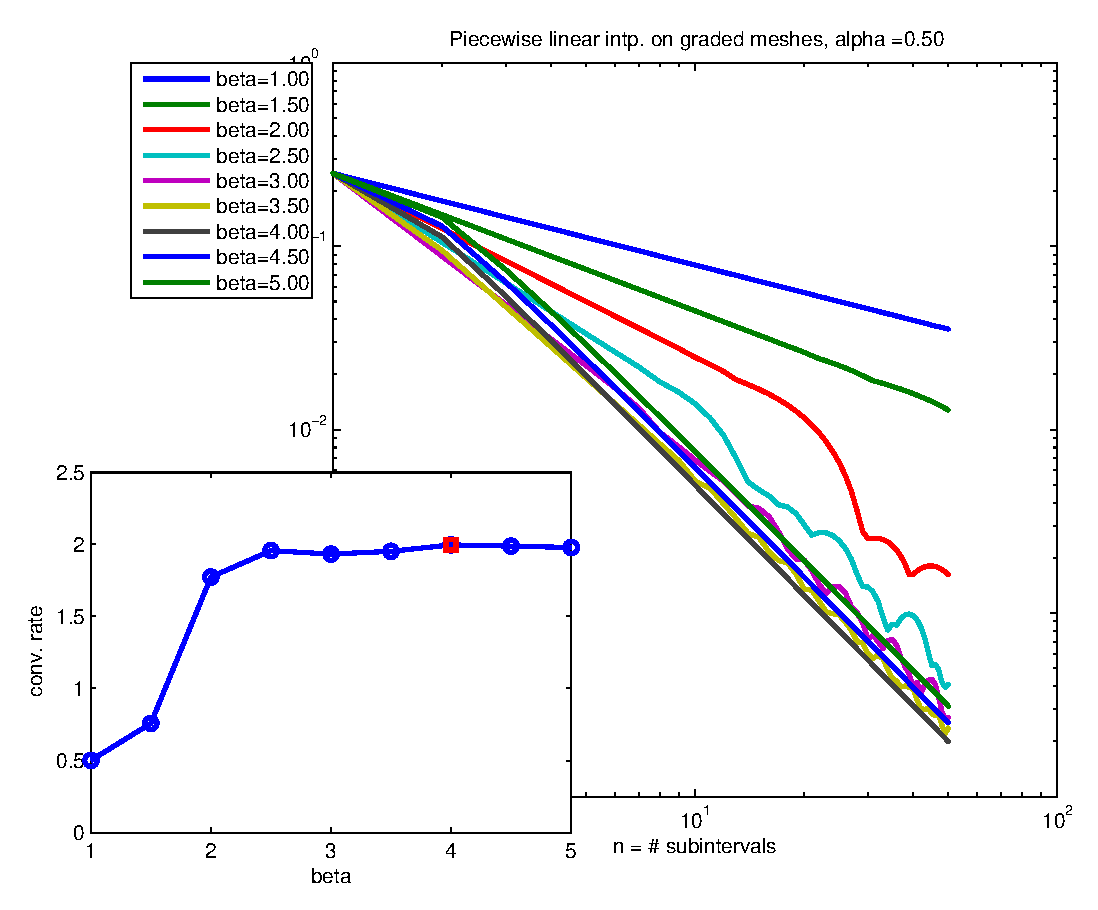
\includegraphics[width=0.85\textwidth]{\problems/ch_piecewisepolynomials/PICTURES/PWlineGraded_050.eps}\end{center}\end{figure}

Figure~\ref{fig:GradedMesh} has been created with the code in Listing~\ref{mc:GradedMesh}.
\lstinputlisting[caption={Plot of algebraically graded mesh.},label={mc:GradedMesh},escapechar={}]
{\problems/ch_piecewisepolynomials/MATLAB/GradedMesh.m}
\end{solution}
\end{subproblem}

\end{problem}

%
\begin{problem}[Chebyshev polynomials and their properties]\label{prob:ChebPolyProp}
  
  Let $T_{n}\in\Pol{n}$ be the $n$-th Chebyshev polynomial, as defined in \lref{def:Tpol} and $\xi_0^{(n)},\dots,\xi_{n-1}^{(n)}$ be the $n$ zeros of $T_n$. According to  \lref{eq:TPN}, these are given by
\begin{equation}\label{eq:zeros}
  \xi^{(n)}_{j} = \cos\left(\frac{2j+1}{2n}\,\pi\right)\;\bcom
    \quad j=0,\ldots,n-1.
\end{equation}
  We define the family of discrete $L^2$ semi inner products, \emph{cf.} \lref{eq:dSPLtwo},
\begin{equation}\label{eq:discrete}
  (f,g)_n:=\sum_{j=0}^{n-1} f(\xi_j^{(n)}) g(\xi_j^{(n)}),\quad f,g\in C^0([-1,1])
\end{equation}
and the special weighted $L^2$ inner product
\begin{equation}\label{eq:weighted}
  (f,g)_w:=\int_{-1}^1 \frac{1}{\sqrt{1-t^2}} f(t) g(t)\,dt \quad f,g\in C^0([-1,1])
\end{equation}

% SUBPROBLEM 1
\begin{subproblem}[2] 
    Show that the Chebyshev polynomials are an orthogonal family of polynomials with respect to the inner product defined in \eqref{eq:weighted} according to \lref{def:onp}, namely $(T_k,T_l)_w=0$ for every $k\neq l$.

    \begin{hint}
      Recall the trigonometric identity $2\cos(x)\cos(y) = \cos(x+y)+\cos(x-y)$.
    \end{hint}

\begin{solution}
For $k,l=0,\dots,n$ with $k\neq l$, by using the substitution $s=\arccos t$ ($ds=- \frac{1}{\sqrt{1-t^2}}\,dt$) and simple trigonometric identities we readily compute
\[
\begin{split}
(T_k,T_l)_w &= \int_{-1}^1 \frac{1}{\sqrt{1-t^2}} \cos(k\,\arccos t) \cos(l\,\arccos t)\,dt \\
&= \int_{0}^\pi  \cos(k s) \cos(l s)\,ds \\
&=\frac{1}{2} \int_{0}^\pi  \cos((k+l) s) + \cos((k-l) s)\,ds \\
&= \frac{1}{2}( [\sin((k+l)s)/(k+l)]^\pi_0 + [\sin((k-l)s)/(k-l)]^\pi_0)\\
&=0,
\end{split}
\]
since $k+l\neq 0$ and $k-l\neq 0$.
\end{solution}
\end{subproblem}

Consider the following statement.

\fbox{\parbox{0.95\textwidth}{
\textbf{Theorem}. The family of polynomials $\{T_0,\dots,T_n\}$ is an orthogonal
basis ($\to$ \lref{def:onb}) 
of $\Pol{n}$ with respect to the inner product $(\; ,\,)_{n+1}$ defined in \eqref{eq:discrete}.
}}

% SUBPROBLEM 2
\begin{subproblem}[2] 
Write a C++ code to test the assertion of the theorem.

\begin{hint}
  \lref{chebpolmult} demonstrates the efficient evaluation of Chebychev
  polynomials based on their 3-term recurrence formula from \lref{rem:3termCheb}.
\end{hint}

   \begin{solution}
As a consequence of \lref{rem:3termCheb}, we already know that $\{T_0,\dots,T_n\}$
is a basis for $\Pol{n}$. We check the orthogonality in the C++ code given in
Listing~\ref{ChebOrthog}.
\lstinputlisting[caption={Orthogonality of Chebyshev polynomials},label={ChebOrthog}]
 {\problems/ch_polynomialinterpolation/CPP/ChebOrthog.cpp}
\end{solution}
\end{subproblem}

% SUBPROBLEM 3
\begin{subproblem}[4] 
Prove the theorem.

\begin{hint}
  Use the relationship of trigonometric functions and the complex exponential
  together with the summation formula for geometric sums. 
\end{hint}

   \begin{solution}
It remains to check the orthogonality condition, namely that $(T_k,T_l)_n=0$ for $k\neq l$. For $k,l=0,\dots,n+1$ with $k\neq l$  by \eqref{eq:zeros}  we have
\begin{equation}\label{eq:norm}
\begin{split}
(T_k,T_l)_{n+1} &= \sum_{j=0}^{n} T_k(\xi_j^{(n)}) T_l(\xi_j^{(n)}) \\
&= \sum_{j=0}^{n} \cos\left(k \frac{2j+1}{2(n+1)}\,\pi\right) \cos\left(l \frac{2j+1}{2(n+1)}\,\pi\right) \\
&=\frac{1}{2} \sum_{j=0}^{n}( \cos\left((k+l) \frac{2j+1}{2(n+1)}\,\pi\right) + \cos\left((k-l) \frac{2j+1}{2(n+1)}\,\pi\right) ).\\
\end{split}
\end{equation}
It is now enough to show that 
\begin{equation}\label{eq:geometric}
\sum_{j=0}^{n} \cos\left(m \frac{2j+1}{2(n+1)}\,\pi\right)=0,\qquad m\in\Z^*.
\end{equation}
In order to verify this, observe that
\[
\sum_{j=0}^{n} \cos \left( m \frac{2j+1}{2(n+1)}\,\pi \right)= 
\Re ( \sum_{j=0}^{n} e^{i m \frac{2j+1}{2(n+1)}\,\pi}  )
= \Re ( e^{i m \frac{1}{2(n+1)}\,\pi} \sum_{j=0}^{n} e^{i m \frac{j}{n+1}\,\pi}  ).
\]
Finally, by the standard formula for the geometric sum we have
\begin{align*}
e^{i m \frac{1}{2(n+1)}\,\pi} \sum_{j=0}^{n} e^{i m \frac{j}{n+1}\,\pi } =e^{i m \frac{1}{2(n+1)}\,\pi}\frac{1-e^{i m \frac{n+1}{n+1}\,\pi} }{1-e^{i m \frac{1}{n+1}\,\pi}} \\
=\frac{1-e^{i m \pi} }{e^{-i m \frac{1}{2(n+1)}\,\pi}-e^{i m \frac{1}{2(n+1)}\,\pi}} = - \frac{1-e^{i m \pi}}{2} \frac{1}{i \sin{m \frac{1}{2(n+1)}\,\pi}} \in i \IR,
\end{align*}
implying $\Re ( e^{i m \frac{1}{2(n+1)}\,\pi} \sum_{j=0}^{n} e^{i m \frac{j}{n+1}\,\pi}  ) = 0$ as desired.
\end{solution}
\end{subproblem}

% SUBPROBLEM 4
\begin{subproblem}[2] 
  Given a function $f\in C^0([-1,1]$, find an expression for the best approximant
  $q_n\in\Pol{n}$ of $f$ in the discrete $L^{2}$-norm:
\[
q_n=\argmin_{p\in\Pol{n}} \norm{f-p}_{n+1},
\]
where $\norm{\;}_{n+1}$ is the norm induced by the scalar product
$(\;,\,)_{n+1}$. You should express $q_n$ through an expansion in Chebychev
polynomials of the form
\begin{equation}\label{eq:alpha}
q_n=\sum_{j=0}^n \alpha_j T_j
\end{equation}
for suitable coefficients $\alpha_j\in\R$.
\begin{hint}
The task boils down to determining the coefficients $\alpha_{j}$. 
Use the theorem you have just proven and a slight extension of \lref{cor:msba:onb}.
\end{hint}
\begin{solution}
In view of the theorem, the family $\{T_0,\dots,T_n\}$ is an orthogonal basis of $\Pol{n}$ with respect to the inner product $(\; ,\,)_{n+1}$. By \eqref{eq:norm} and \eqref{eq:geometric} we have
\begin{equation}\label{eq:lambda}
\lambda_k^2:=\norm{T_k}^2_{n+1}=(T_k,T_k)_{n+1}=
\begin{cases}
\frac{1}{2}\sum_{j=0}^n(\cos(0) + \cos(0))=n+1 & \text{if $k=0$},\\
\frac{1}{2}\sum_{j=0}^n \cos(0)=(n+1)/2 & \text{otherwise.}
\end{cases}
\end{equation}
The family $\{T_k/\lambda_k:k=0,\dots,n\}$ is an ONB of $\Pol{n}$ with respect to the inner product $(\; ,\,)_{n+1}$. Hence, by \lref{cor:msba:onb} we have that
\[
q_n=\sum_{j=0}^n\, (f,T_j/\lambda_j)_{n+1}\, \frac{T_j}{\lambda_j}=\sum_{j=0}^n \alpha_j T_j,\quad \alpha_j=\frac{1}{n+1}
\begin{cases}
{(f,T_j)_{n+1}} & \text{if $k=0$},\\
2 {(f,T_j)_{n+1}}& \text{otherwise.}
\end{cases}
\]
\end{solution}
\end{subproblem}

% SUBPROBLEM 5
\begin{subproblem}[2]
Write a C++ function
\begin{lstlisting}
template <typename Function>
void bestpolchebnodes(const Function &f, Eigen::VectorXd &alpha)
\end{lstlisting}
that returns the vector of coefficients $(\alpha_j)_j$ in \eqref{eq:alpha} given a function $f$. Note that the degree of the polynomial is indirectly passed with the length of the output \texttt{alpha}. The input \texttt{f} is a lambda-function, e.g.
\begin{lstlisting}
auto f = [] (double & x) {return 1/(pow(5*x,2)+1);};
\end{lstlisting}


\begin{solution}
See file \texttt{ChebBest.cpp}.
\end{solution}
\end{subproblem}

% SUBPROBLEM 6
\begin{subproblem}[2] 
Test \texttt{bestpolchebnodes} with the function $f(x)=\frac{1}{(5x)^2+1}$ and
$n=20$. Approximate the supremum norm of the approximation error by sampling on an
equidistant grid with $10^{6}$ points. 

\begin{hint}
  Again, \lref{chebpolmult} is useful for evaluating Chebychev polynomials. 
\end{hint}


% Copy and paste the vector of coefficients obtained to Matlab and plot the result, comparing it with $f$. Use the Matlab built-in function \texttt{chebyshevT}.
   \begin{solution}
See file \texttt{ChebBest.cpp}. The output (plotted with Matlab) is shown in Figure~\ref{fig:ChebBest}.
\begin{figure}\begin{center}
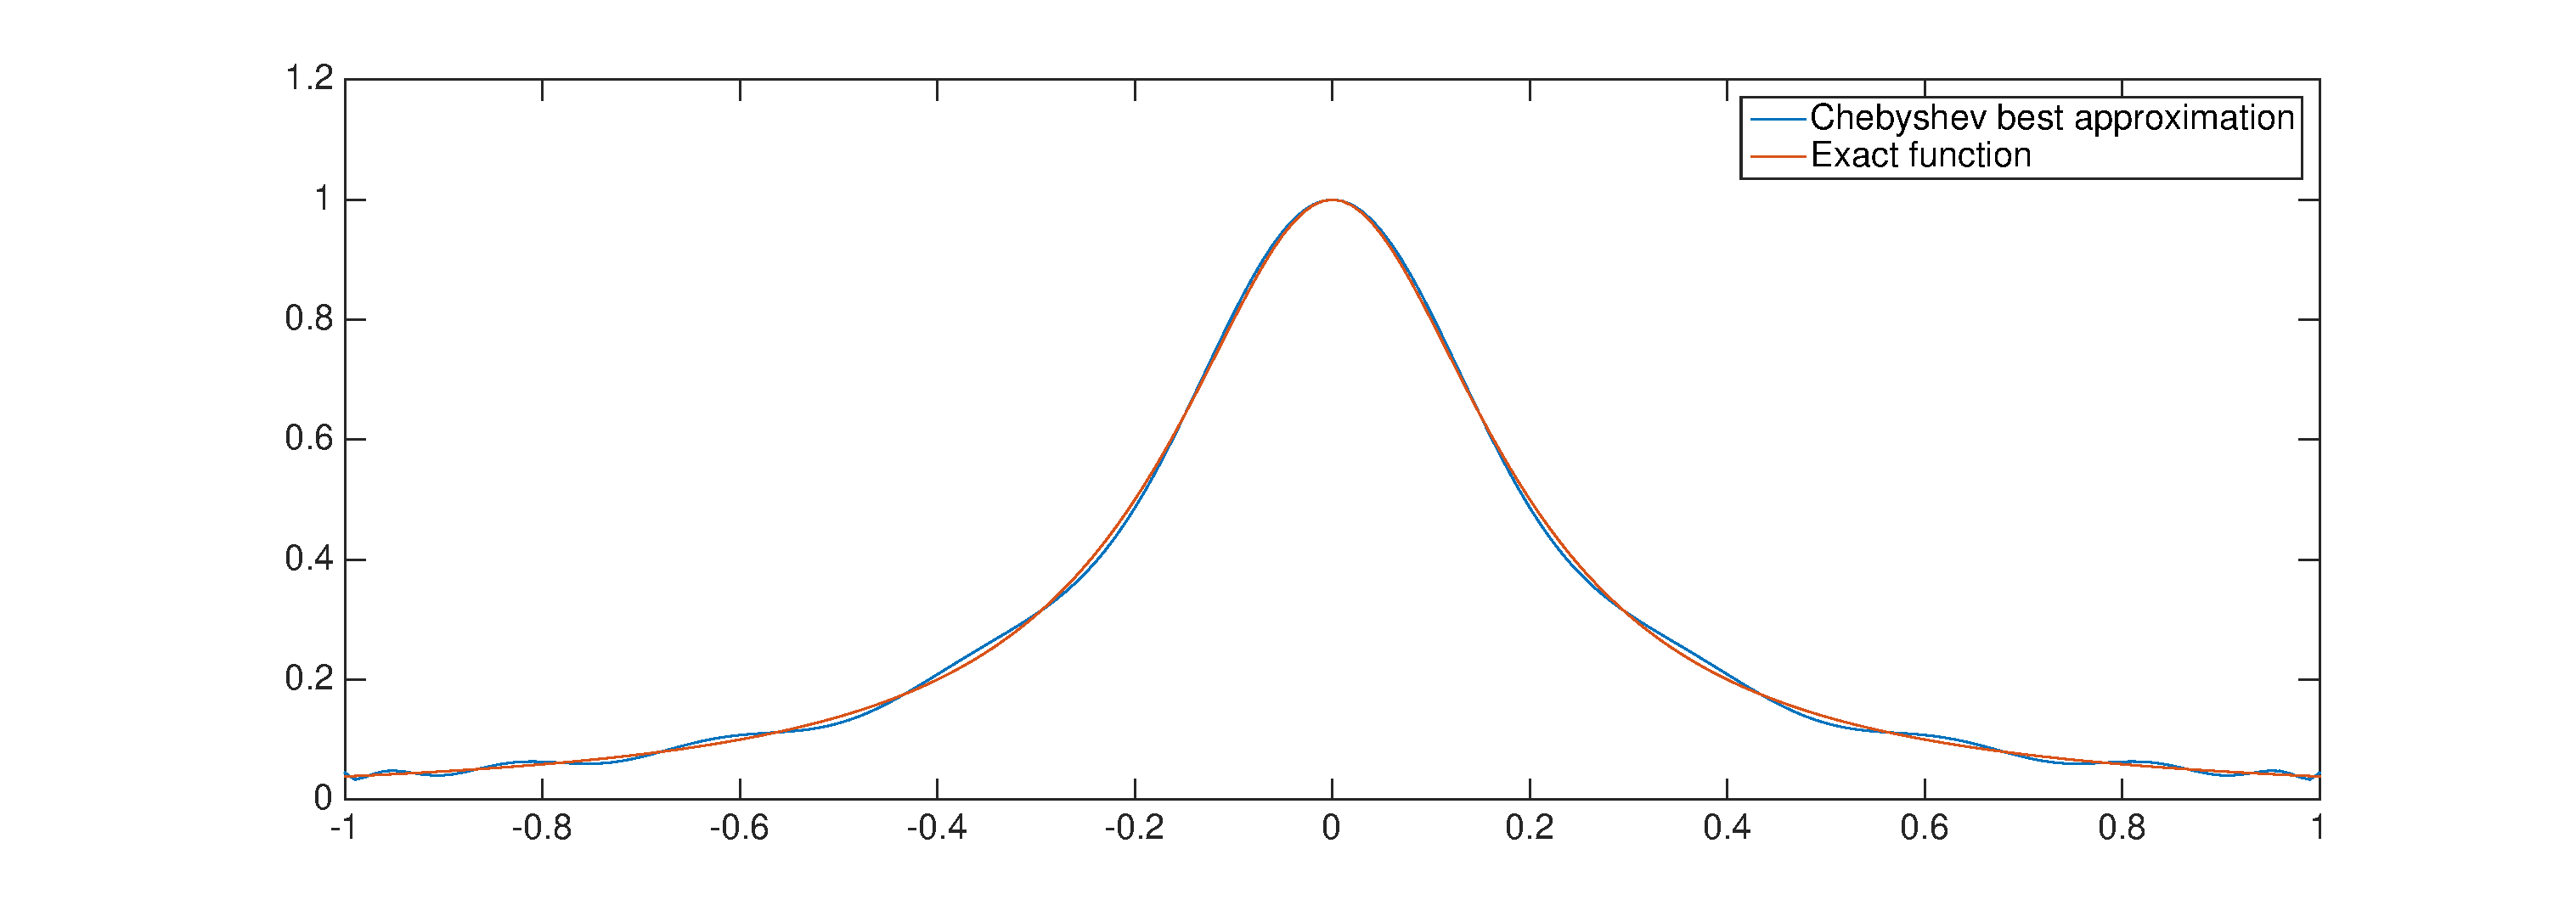
\includegraphics[width = \textwidth]{\problems/ch_polynomialinterpolation/PICTURES/ChebBest.eps}
\caption{The result of code \texttt{ChebBest.m}.}
\label{fig:ChebBest}
\end{center}\end{figure}
\end{solution}
\end{subproblem}

% SUBPROBLEM 7
\begin{subproblem}[2] 
Let $L_j$, $j=0,\dots,n$, be the Lagrange polynomials associated with the nodes
$t_j=\xi^{(n+1)}_{j}$ of Chebyshev interpolation with $n+1$ nodes on $[-1,1]$, see
\lref{eq:TPN}. Show that
\[
L_j = \frac{1}{n+1} + \frac{2}{n+1} \sum_{l=1}^n T_l(\xi^{(n+1)}_{j}) T_l.
\]

\begin{hint}
  Again use the above theorem to express the coefficients of a Chebychev expansion
  of  $L_{j}$. 
\end{hint}

   \begin{solution}
We have already seen that $\{T_l/\lambda_l:l=0,\dots,n\}$ is an ONB of $\Pol{n}$. Thus we can write
\[
L_j=\sum_{l=0}^n \frac{(L_j,T_l)_{n+1}}{\lambda_l^2} T_l =\sum_{l=0}^n \sum_{k=0}^n L_j(\xi^{(n+1)}_{k}) T_l(\xi^{(n+1)}_{k}) \frac{T_l}{\lambda_l^2} 
\]
By definition of Lagrange polynomials we have $ L_j(\xi^{(n+1)}_{k}) = \delta_{jk}$, whence
\[
L_j=\sum_{l=0}^n  T_l(\xi^{(n+1)}_{l}) \frac{T_l}{\lambda_l^2}.
\]
Finally, the conclusion immediately follows from \eqref{eq:lambda}.
\end{solution}
\end{subproblem}

\end{problem}





\begin{problem}[Piecewise cubic Hermite interpolation]
 
 Piecewise cubic Hermite interpolation with exact slopes on a mesh
 \[
\mathcal{M} := \{ a = x_0 < x_1 < \dots < x_n = b \}
 \]
 was defined in \ncseref{sec:HermiteInterpolation}. For $f \in C^4([a,b])$ it
 enjoys $h$-convergence with rate $4$ as we have seen in \lref{ex:hermcvg1}.
 
 Now we consider cases, where perturbed or reconstructed slopes are used. For
 instance, this was done in the context of monotonicity preserving piecewise cubic
 Hermite interpolation as discussed in \lref{sec:hipshp}.
 
 \begin{subproblem}[2] \label{subprb:pchi_1}
  Assume that piecewise cubic Hermite interpolation is based on perturbed slopes, that is, the piecewise cubic function $s$ on $\mathcal{M}$ satisfies:
  \begin{align*}
   s(x_j) = f(x_j)\quad,\quad s'(x_j) = f'(x_j) + \delta_j,
  \end{align*}
  where the $\delta_j$ may depends on $\mathcal{M}$, too.
  
  Which rate of asymptotic $h$-convergence of the $\sup$-norm of the approximation error can
  be expected, if we know that for all $j$
  
  \begin{align*}
   \lvert \delta_j \rvert = O(h^\beta)\;,\quad \beta \in \IN_0\;,
  \end{align*}
  for mesh-width $h \rightarrow 0$.
  
  \begin{hint}
   Use a local generalized cardinal basis functions, cf. \ncseref{par:pchiploc}.
  \end{hint}
  
  \begin{solution}
   Let $s$ be the piecewise cubic polynomial interpolant of $f$. We can rewrite $s$ using the local representation with cardinal basis:
   \begin{align*}
    s(t) & = y_{i-1} H_1(t) + y_i H_2(t) + c_{i-1} H_3(t) + c_i H_4(t) \\
     & = y_{i-1} H_1(t) + y_i H_2(t) + (f'(t_{i-1}) + \delta_{i-1}) H_3(t) + (f'(t_i) + \delta_i) H_4(t) \\
     & = y_{i-1} H_1(t) + y_i H_2(t) + f'(t_{i-1}) H_3(t) + f'(t_i)  H_4(t) + \delta_{i-1} H_3(t) + \delta_i H_4(t)
   \end{align*}
   Hence, if we denote by $\tilde{s}$ the Hermite interpolant with exact slopes:
   \begin{align*}
    \lVert f - s \rVert_{L^\infty([a,b])} & \leq \lVert f - \tilde{s} + \tilde{s} - s \rVert_{L^\infty([a,b])} \leq \lVert f - \tilde{s} \rVert_{L^\infty([a,b])} + \lVert \tilde{s} - s \rVert_{L^\infty([a,b])} \\
    & \leq O(h^4) + \max_{i} \lVert \delta_{i-1} H_3(t) + \delta_i H_4(t) \rVert_{L^\infty([t_{i-1},t_i])} \\
    & = O(h^4) + O(h^{b+1}) = O(\min(4,\beta + 1))
   \end{align*}
  since $\lVert H_3(t) \rVert_{L^\infty([t_{i-1},t_i])} = \lVert H_4(t) \rVert_{L^\infty([t_{i-1},t_i])} = O(h)$ (attain maximum at $t = \frac{1}{3h}(t_{i} - t)$ resp. minimum at $t = \frac{2}{3h}(t_{i} - t)$, with value $h (\left(\frac{2}{3}\right)^3 - \left(\frac{2}{3}\right)^2)$).
  \end{solution}

 \end{subproblem}

 \begin{subproblem}[3]
  Implement a strange piecewise cubic interpolation scheme in \Cpp{} that satisfies:
  \begin{align*}
   s(x_j) = f(x_j)\quad,\quad s'(x_j) = 0
  \end{align*}
  and empirically determine its convergence on a sequence of equidistant meshes of $[-5,5]$ with mesh-widths $h = 2^{-l}, l = 0,\dots,8$ and for the interpoland $f(t) := \frac{1}{1+t^2}$.
  
  As a possibly useful guideline, you can use the provided \Cpp{} template, see the file \verb|piecewise_hermite_interpolation_template.cpp|.
   
  Compare with the insight gained in \ref{subprb:pchi_1}.
  
\cprotEnv \begin{solution}
   According to the previous subproblem, since $s'(x_j) = f'(x_j) - f'(x_j)$, i.e. $\lvert \delta_j \rvert = O(1)$, $\beta = 0$, the convergence order is limited to $O(h)$.
   
   For the \Cpp{} solution, cf. \verb|piecewise_hermite_interpolation.cpp|.
  \end{solution}
 \end{subproblem}

 \begin{subproblem}[1]
   Assume equidistant meshes and reconstruction of slopes by a particular
   averaging. More precisely,
   the $\mathcal{M}$-piecewise cubic function $s$ is to satisfy the generalized 
   interpolation conditions
  \begin{align*}
   s(x_j) & = f(x_j), \\
   s'(x_j) & = \begin{cases}
              \frac{-f(x_2) + 4f(x_1) - 3f(x_0)}{2h} &\text{for } j = 0\;, \\
              \frac{f(x_{j+1}) - f(x_{j-1})}{2h} &\text{for } j = 1,\dots,n-1\;, \\
              \frac{3f(x_n) - 4f(x_{n-1}) + f(x_{n-2})}{2h} &\text{for } j = n\;. \\
             \end{cases}
  \end{align*}
  What will be the rate of $h$-convergence of this scheme (in $\sup$-norm)?
  
  (You can solve this exercise either theoretically or  determine an empiric convergence rate in a numerical experiment.)
  
  \begin{hint}
    If you opt for the theoretical approach, you can
    use what you have found in \autoref{subprb:pchi_1}. To find perturbation
    bounds, rely on the Taylor expansion formula with remainder, see
    \lref{ex:taylorcancel}. 
  \end{hint}
  
\cprotEnv \begin{solution}
   First, we show that the approximation $s'(x_j) = f'(x_j) + O(h^2)$. This follows from Taylor expansion:
   \begin{align*}
    f(x) = f(x_j) + f'(x_j) ( x - x_j ) + f''(x_j) (x - x_j)^2 / 2 + O(h^3)
   \end{align*}
  Using $x = x_{j-1}$ and $x = x_{j+1}$ (and $h = x_{j+1}- x_j$):
   \begin{align*}
    \frac{f(x_{j+1}) - f(x_{j})}{h} = f'(x_j) + f''(x_j) h / 2 + O(h^2) \\
    \frac{f(x_{j-1}) - f(x_{j})}{h} = -f'(x_j) + f''(x_j) h / 2 + O(h^2)
   \end{align*}
   Subtracting the second equation to the first equation:
   \begin{align*}
    \frac{f(x_{j+1}) - f(x_{j-1})}{h} = 2f'(x_j) + O(h^2)
   \end{align*}
   For the one-sided difference we expand at $x = x_{j+2}$ and $x = x_{j+1}$:
   \begin{align*}
    \frac{f(x_{j+1}) - f(x_{j})}{h} = f'(x_j) + f''(x_j) h / 2 + O(h^2) \\
    \frac{f(x_{j+2}) - f(x_{j})}{2h} = f'(x_j) + f''(x_j) h + O(h^2)
   \end{align*}
   Subtracting the first equation to half of the second equation:
   \begin{align*}
    \frac{f(x_{j+2}) - f(x_{j})}{4h} - \frac{f(x_{j+1}) - f(x_{j})}{h} = f'(x_j) (1/2 - 1) + O(h^2) \\
    \frac{f(x_{j+1}) - f(x_{j}) - 4 f(x_{j+1}) + 4 f(x_{j})}{4h} = f'(x_j) (1/2 - 1) + O(h^2) \\
    \frac{- f(x_{j+2}) + 4 f(x_{j+1}) - 3 f(x_{j})}{2h} = f'(x_j) + O(h^2) \\
   \end{align*}
   The other side is analogous.

   According to the previous subproblem, since $s'(x_j) = f'(x_j) + O(h^2)$ and $\beta = 2$, the convergence order is limited to $O(h^3)$.
   
   For the \Cpp{} solution, cf. \verb|piecewise_hermite_interpolation.cpp|.
  \end{solution}
 \end{subproblem}

 
\end{problem}

\end{sheet}

%%% PS10
\begin{sheet}{10}{19.11.2015}{26.11.2015}
% ncse_new/\problems/ch_piecewisepolynomials/ex_CubicSplines.tex
%  solution:  ex_CubicSpline.m  ex_CubicSpline.eps

\begin{problem}[Zeros of orthogonal polynomials \coreproblem]
 This problem combines elementary methods for zero finding with 3-term recursions satisfied by orthogonal polynomials. 
  
The zeros of the Legendre polynomial $P_n$ (see \lref{def:Legendrepol}) are the $n$ Gauss points $\xi^n_j$, $j=1,\dots,n$. In this problem we compute the Gauss points by zero finding methods applied to $P_n$. The 3-term recursion \lref{eq:Legpol} for Legendre polynomials will play an essential role. Moreover, recall that, by definition, the Legendre polynomials are $L^2(]-1,1[)$-orthogonal.

% SUBPROBLEM 1
\begin{subproblem}[5]\label{subpb:inter}
Prove the following interleaving property of the zeros of the Legendre polynomials. For all $n\in\n_0$ we have
\begin{equation*}
-1<\xi^n_j<\xi^{n-1}_j<\xi^n_{j+1}<1,\qquad j=1,\dots,n-1.
\end{equation*}
 \begin{hint}
You may follow these steps:
\begin{enumerate}\itemsep0pt
\item Understand that it is enough to show that every pair of zeros $(\xi^n_l,\xi^n_{l+1})$ of $P_n$ is separated by a zero of $P_{n-1}$.
\item Argue by contradiction.
\item By considering the auxiliary polynomial $\prod_{j\neq l,l+1} (t-\xi_j^n)$ and the fact that the Gauss quadrature is exact on $\Pol{2n-1}$ prove that $P_{n-1}(\xi_l^n)=P_{n-1}(\xi_{l+1}^n)=0$.
\item Choose $s\in \Pol{n-2}$ such that $s(\xi^n_j)=P_{n-1}(\xi_j^n)$ for every $j\neq l,l+1$, and using again that  Gauss quadrature is exact on $\Pol{2n-1}$ obtain a contradiction.
\end{enumerate}
\end{hint}

\begin{solution}
By \lref{lem:gn}, $P_n$ has exactly $n$ distinct zeros in $]-1,1[$. Therefore, it is enough to prove that every pair of zeros of $P_n$ is separated by one zero of $P_{n-1}$. By contradiction, assume that there exists $l=1,\dots,n-1$ such that $]\xi^n_l,\xi_{l+1}^n[$ does not contain any zeros of $P_{n-1}$. As a consequence, $P_{n-1}(\xi^n_l)$ and $P_{n-1}(\xi^n_{l+1})$ have the same sign, namely
\begin{equation}\label{eq:separate}
P_{n-1}(\xi^n_l) P_{n-1}(\xi^n_{l+1})\ge 0.
\end{equation}

Recall that, by construction, we have the following orthogonality property
\begin{equation}\label{eq:orthog}
\int_{-1}^1P_{n-1}q\,dt=0,\qquad q\in\Pol{n-2}.
\end{equation}

Consider the auxiliary polynomial
\[
q(t)=\prod_{j\neq l,l+1} (t-\xi^n_j).
\]
By construction, $q\in\Pol{n-2}$, whence $P_{n-1}q\in\Pol{2n-3}$. Thus, using \eqref{eq:orthog} and the fact that Gaussian quadrature is exact on $P_{2n-1}$ we obtain
\[
0 = \int_{-1}^1P_{n-1}q\,dt 
 = \sum_{j=1}^n w_j P_{n-1}(\xi_j^n) q(\xi^n_j) 
 = w_l P_{n-1}(\xi_l^n) q(\xi^n_l) + w_{l+1} P_{n-1}(\xi_{l+1}^n) q(\xi^n_{l+1}).
\]
Hence
\[
\left[ w_l P_{n-1}(\xi_l^n) q(\xi^n_l) \right] \left[ w_{l+1} P_{n-1}(\xi_{l+1}^n) q(\xi^n_{l+1})\right]\le 0.
\]
On the other hand, by \lref{lem:gw} we have $w_l ,w_{l+1}>0$. Moreover, by construction of $q$ we have that $q(\xi^n_l)q(\xi^n_{l+1})>0$. Combining these properties with \eqref{eq:separate} we obtain that
\[
P_{n-1}(\xi_l^n)=P_{n-1}(\xi_{l+1}^n)=0.
\]

Choose now $s\in \Pol{n-2}$ such that $s(\xi^n_j)=P_{n-1}(\xi_j^n)$ for every $j\neq l,l+1$. Using again \eqref{eq:orthog} and the fact that Gaussian quadrature is exact on $P_{2n-1}$ we obtain
\[
0=\int_{-1}^1 P_{n-1} s\,dt=\sum_{j=1}^n w_j P_{n-1}(\xi_j^n) s(\xi_j^n)= \sum_{j\neq l,l+1} w_j (P_{n-1}(\xi_j^n))^2.
\]
Since $P_{n-1}$ has only $n-1$ zeros and the weights $w_j$ are all positive, the right hand side of this equality is strictly positive, thereby contradicting the equality itself.

\textbf{Solution 2: }
There is a shorter proof of this fact based on the recursion formula \lref{eq:Legpol}. We sketch the main steps.

We will prove the statement by induction. If $n=1$ there is nothing to prove. Suppose now that the statement is true for $n$. By \lref{eq:Legpol} we have $P_{n+1}(\xi^n_j)=-\frac{n}{n+1}P_{n-1}(\xi^n_j)$ for every $j=1,\dots,n$. Further, since the statement is true for $n$ we have $(-1)^{n-j}P_{n-1}(\xi^n_j)>0$. Therefore
\begin{equation}\label{eq:last}
(-1)^{n+1-j}P_{n+1}(\xi^n_j)>0,\qquad j=1,\dots,n.
\end{equation}
Since the leading coefficient of $P_{n+1}$ is positive, we have $P_{n+1}(x)>0$ for all $x>\xi^{n+1}_{n+1}$ and $(-1)^{n+1}P_{n+1}(x)>0$ for all $x<\xi^{n+1}_{1}$. Combining these two inequalities with \eqref{eq:last} yields the result for $n+1$.
\end{solution}
\end{subproblem}


% SUBPROBLEM 2
\begin{subproblem}[1]\label{subpb:2}
By differentiating \lref{eq:Legpol} derive a combined 3-term recursion for the sequences $(P_n)_n$ and $(P'_n)_n$.
\begin{solution}
Differentiating \lref{eq:Legpol} immediately gives
\begin{equation*}
P_{n+1}'(t)=\frac{2n+1}{n+1}P_n(t) + \frac{2n+1}{n+1} t P_n'(t)-\frac{n}{n+1}P'_{n-1}(t),\quad P_0'=0,\quad P_1'=1,
\end{equation*}
which combined with \lref{eq:Legpol} gives the desired recursions.
\end{solution}
\end{subproblem}

% SUBPROBLEM 3
\begin{subproblem}[2]
Use the recursions obtained in \ref{subpb:2} to write a C++ function
\begin{lstlisting}
void legvals(const Eigen::VectorXd &x, Eigen::MatrixXd &Lx, Eigen::MatrixXd &DLx)
\end{lstlisting}
that fills the matrices \texttt{Lx} and \texttt{DLx} in $\R^{N\times (n+1)}$ with the values $(P_k(x_j))_{jk}$ and $(P'_k(x_j))_{jk}$, $k=0,\dots,n$, $j=0,\dots,N-1$, for an input vector $x\in \R^N$ (passed in \texttt{x}).
\begin{solution}
See file \texttt{legendre.cpp}.
\end{solution}
\end{subproblem}

% SUBPROBLEM 4
\begin{subproblem}[3]
We can compute the zeros of $P_k$, $k=1,\dots,n$, by means of the secant rule (see \lref{par:secant}) using the endpoints $\{-1,1\}$ of the interval and the zeros of the previous Legendre polynomial as initial guesses, see \ref{subpb:inter}. We opt for a correction based termination criterion (see \lref{sec:termination-criteria-1}) based on prescribed relative and absolute tolerance (see \lref{mc:secant}).

Write a C++ function
\begin{lstlisting}
MatrixXd gaussPts(int n, double rtol=1e-10, double atol=1e-12)
\end{lstlisting}
that computes the Gauss points $\xi^k_j\in [-1,1]$, $j=1,\dots,k$, $k=1,\dots,n$, using the zero finding approach outlined above. The Gauss points should be returned in  an upper triangular $n\times n$-matrix.
\begin{hint}
For simplicity, you may want to write a C++ function
\begin{lstlisting}
double Pkx(double x, int k)
\end{lstlisting}
that computes $P_k(x)$ for a scalar $x$. Reuse parts of the function \texttt{legvals}.
\end{hint}
\begin{solution}
See file \texttt{legendre.cpp}.
\end{solution}
\end{subproblem}

% SUBPROBLEM 5
\begin{subproblem}[2]
Validate your implementation of the function \texttt{gaussPts} with $n=8$ by computing the values of the Legendre polynomials in the zeros obtained (use the function \texttt{legvals}). Explain the failure of the method.
\begin{hint}
See Figure~\ref{fig:secant}.
\begin{figure}[hbt]
\hspace{8mm}
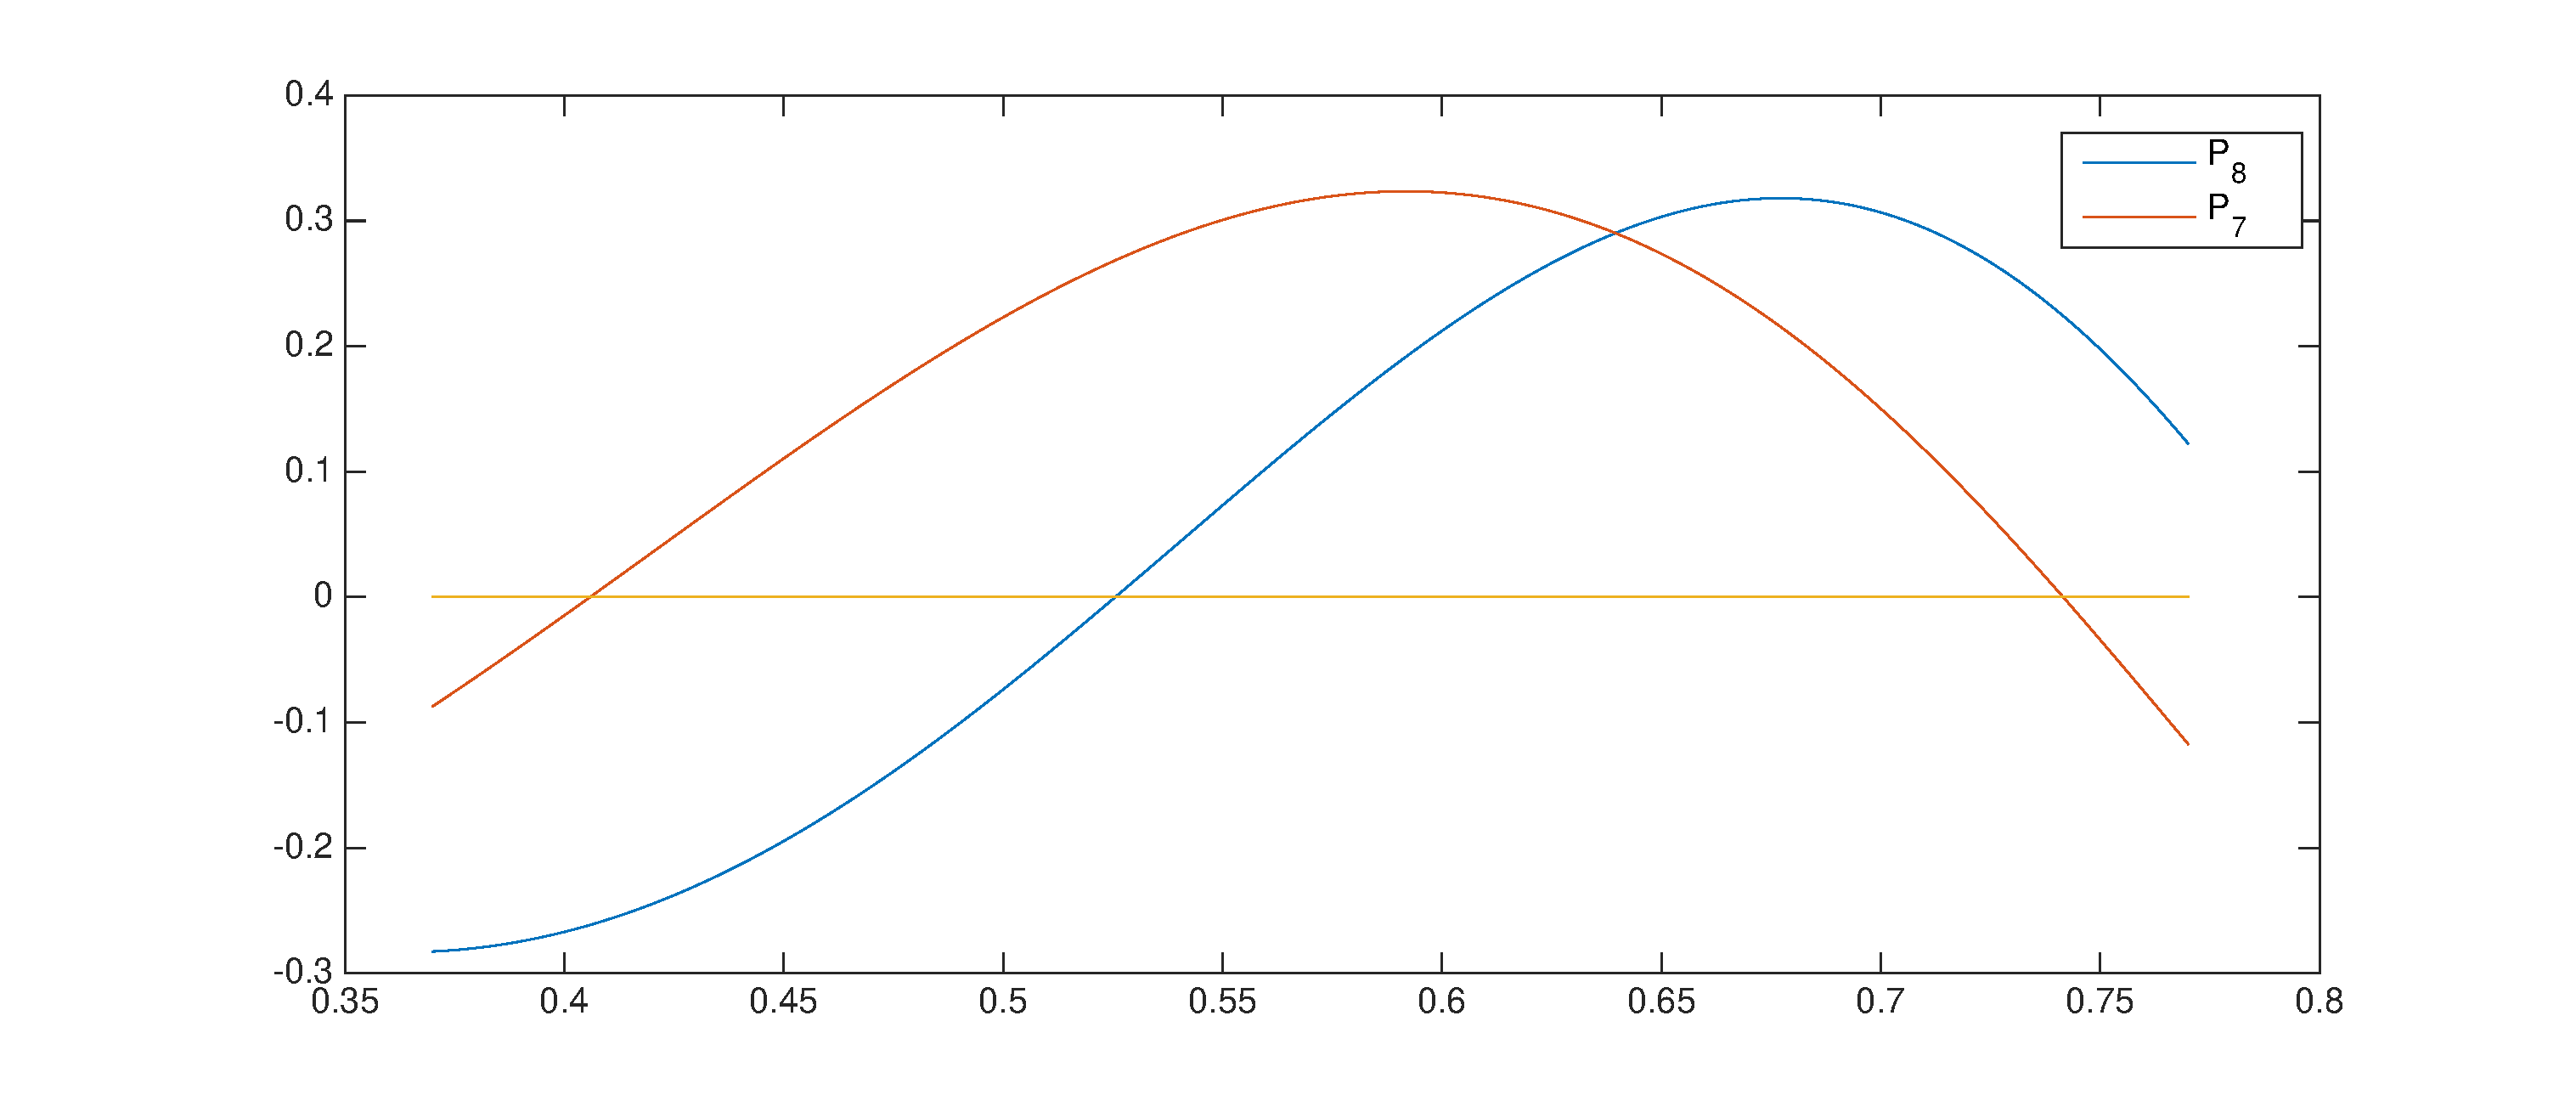
\includegraphics[width=.9\textwidth]{\problems/ch_numericalquadrature/PICTURES/secant.eps}
\caption{$P_7$ and $P_8$ on a part of $[-1,1]$. The secant method fails to find the zeros of $P_8$ (blue curve) when started with the zeros of $P_7$ (red curve).}
\label{fig:secant}
\end{figure}
\end{hint}
\begin{solution}
See file \texttt{legendre.cpp} for the implementation. The zeros of $P_k$, $k=1,\dots,7$ are all correctly computed, but the zero $\xi^8_6\approx 0.525532$ of $P_8$ is not correct. This is due to the fact that in this case the initial guesses for the secant method are not close enough to the zero (remember, only local convergence is guaranteed). Indeed, taking $x^{(0)}$ and $x^{(1)}$ as the two consecutive zeros of $P_7$ in Figure~\ref{fig:secant}, the third iterate $x^{(2)}$ will satisfy $P_8(x^{(1)})P_8(x^{(2)})>0$ and the forth iterate will be very far from the desired zero.
\end{solution}
\end{subproblem}

% SUBPROBLEM 6
\begin{subproblem}[2]
Fix your function \texttt{gaussPts} taking into account the above considerations. You should use the \emph{regula falsi}, that is a variant of the secant method in which, at each step, we choose the old iterate to keep depending on the signs of the function. More precisely, given two approximations $x^{(k)}$, $x^{(k-1)}$ of a zero in which the function $f$ has different signs, compute another approximation $x^{(k+1)}$ as zero of the secant. Use this as the next iterate, but then chose as $x^{(k)}$ the value $z \in \{ x^{(k)} ,x^{(k-1)}\}$ for which $ {\rm sign} f(x^{(k+1)}) \neq {\rm sign} f(z)$. This ensures that $f$ has always a different sign in the last two iterates.
\begin{hint}
The regula falsi variation of the secant method can be easily implemented with a little modification of \lref{mc:secant}:
\begin{lstlisting}
function x = secant_falsi(x0,x1,F,rtol,atol)
fo = F(x0);
for i=1:MAXIT
  fn = F(x1);
  s = fn*(x1-x0)/(fn-fo); % correction
  if (F(x1 - s)*fn < 0)
    x0 = x1;  fo = fn;  end
  x1 = x1 - s;
  if (abs(s) < max(atol,rtol*min(abs([x0;x1]))))
    x = x1; return; end
end  
  \end{lstlisting}
\end{hint}
\begin{solution}
See file \texttt{legendre.cpp}.
\end{solution}
\end{subproblem}

\end{problem}





% ncse_new/p2_InterpolationApproximation/ch4_NumericalQuadrature/ex_GaussianQuadrature.tex
% exercise requires:   gaussquad.m    GaussArcSin.p    GaussArcSinCV.p
% solutions require:   GaussConv.m    GaussConv.eps    GaussConvCV.m    GaussConvCV.eps

\begin{problem}[Gaussian quadrature \coreproblem] \label{prb:GaussianQuadrature}

Given a smooth, odd function $f:[-1,1]\rightarrow\IR$, consider the integral
\begin{equation}
\label{eq:GaussianQuadrature_IntArcsin}
I := \int_{-1}^{1} \arcsin(t) \; f(t) \,\mathrm{d}t.
\end{equation}
We want to approximate this integral using global Gauss quadrature.
The nodes (vector \texttt{x}) and the weights (vector \texttt{w}) of $n$-point Gaussian quadrature on $[-1,1]$ can be computed using the provided \Matlab{} routine \texttt{[x,w]=gaussquad(n)} (in the file \texttt{gaussquad.m}).

%%%%%%%%%%%% SUBPROBLEM 1

\begin{subproblem}[3] \label{subprb:GaussianQuadrature_1}
Write a \Matlab{} routine
\begin{center}
\texttt{function \quad GaussConv(f\_hd)}
\end{center}
that produces an appropriate convergence plot of the quadrature error versus the
number $n=1,\ldots,50$ of quadrature points. Here, \texttt{f\_hd} is a handle to
the function $f$.

Save your convergence plot for $f(t)=\sinh(t)$ as \texttt{GaussConv.eps}.
\begin{hint}
Use the \Matlab{} command \texttt{quad} with tolerance \texttt{eps} to compute a reference value of the integral.
\end{hint}

\begin{hint}
If you cannot implement the quadrature formula, you can resort to the \Matlab{} function
\begin{center}
\texttt{function \quad I = GaussArcSin(f\_hd,n)}
\end{center}
provided in implemented \texttt{GaussArcSin.p} that computes $n$-points Gauss
quadrature for the integral~\eqref{eq:GaussianQuadrature_IntArcsin}. Again \texttt{f\_hd} is a
function handle to $f$.
\end{hint}

\cprotEnv \begin{solution}
See \autoref{mc:GaussianQuadrature_GaussConv} and \autoref{fig:GaussianQuadrature_GaussConv}:
\lstinputlisting[caption={implementation for the function \texttt{GaussConv}},label={mc:GaussianQuadrature_GaussConv},escapechar={}]
{\problems/ch_numericalquadrature/MATLAB/GaussConv.m}
\begin{figure}
\centering
\includegraphics[width=0.6\textwidth]{\problems/ch_numericalquadrature/PICTURES/GaussConv.eps}
\caption{Convergence of \texttt{GaussConv.m}.}
\label{fig:GaussianQuadrature_GaussConv}
\end{figure}
\end{solution}
\end{subproblem}

%%%%%%%%%%%% SUBPROBLEM 2

\begin{subproblem}[1] \label{subprb:GaussianQuadrature_2}
Which kind of convergence do you observe?

\begin{solution}
Algebraic convergence, approximately $O(n^{-2.7})$.
\end{solution}
\end{subproblem}

%%%%%%%%%%%% SUBPROBLEM 3

\begin{subproblem}[2] \label{subprb:GaussianQuadrature_3}
Transform the integral
\eqref{eq:GaussianQuadrature_IntArcsin} into an equivalent one with a suitable change of variable so that Gauss quadrature
applied to the transformed integral converges much faster.

\begin{solution}
With the change of variable $t=\sin(x)$, $\mathrm{d}t=\cos x\mathrm{d}x$
$$I = \int_{-1}^{1} \arcsin(t)\; f(t) \,\mathrm{d}t  = \int_{-\pi/2}^{\pi/2} x\; f(\sin(x))\cos(x)\,\mathrm{d}x.$$
(the change of variable has to provide a smooth integrand on the integration interval)
\end{solution}
\end{subproblem}

%%%%%%%%%%%% SUBPROBLEM 4

\begin{subproblem}[3] \label{subprb:GaussianQuadrature_4}
Now, write a \Matlab{} routine
\begin{center}
\texttt{function\quad GaussConvCV(f\_hd)}
\end{center}
which plots the quadrature error versus the number $n=1,\ldots,50$ of quadrature points for the integral obtained in the previous subtask.

Again, choose $f(t)=\sinh(t)$ and save your convergence plot as \texttt{GaussConvCV.eps}.

\begin{hint}
In case you could not find the transformation, you may rely on the function
\end{hint}
\begin{center}
\texttt{function \quad I = GaussArcSinCV(f\_hd,n)}
\end{center}
implemented in \texttt{GaussArcSinCV.p} that applies $n$-points Gauss quadrature
to the transformed problem.

\begin{solution}
See \autoref{mc:GaussianQuadrature_GaussConvCV} and \autoref{fig:GaussianQuadrature_GaussConvCV}:
\lstinputlisting[caption={implementation for the function \texttt{GaussConvCV}},label={mc:GaussianQuadrature_GaussConvCV},escapechar={}]
{\problems/ch_numericalquadrature/MATLAB/GaussConvCV.m}
\begin{figure}
\centering
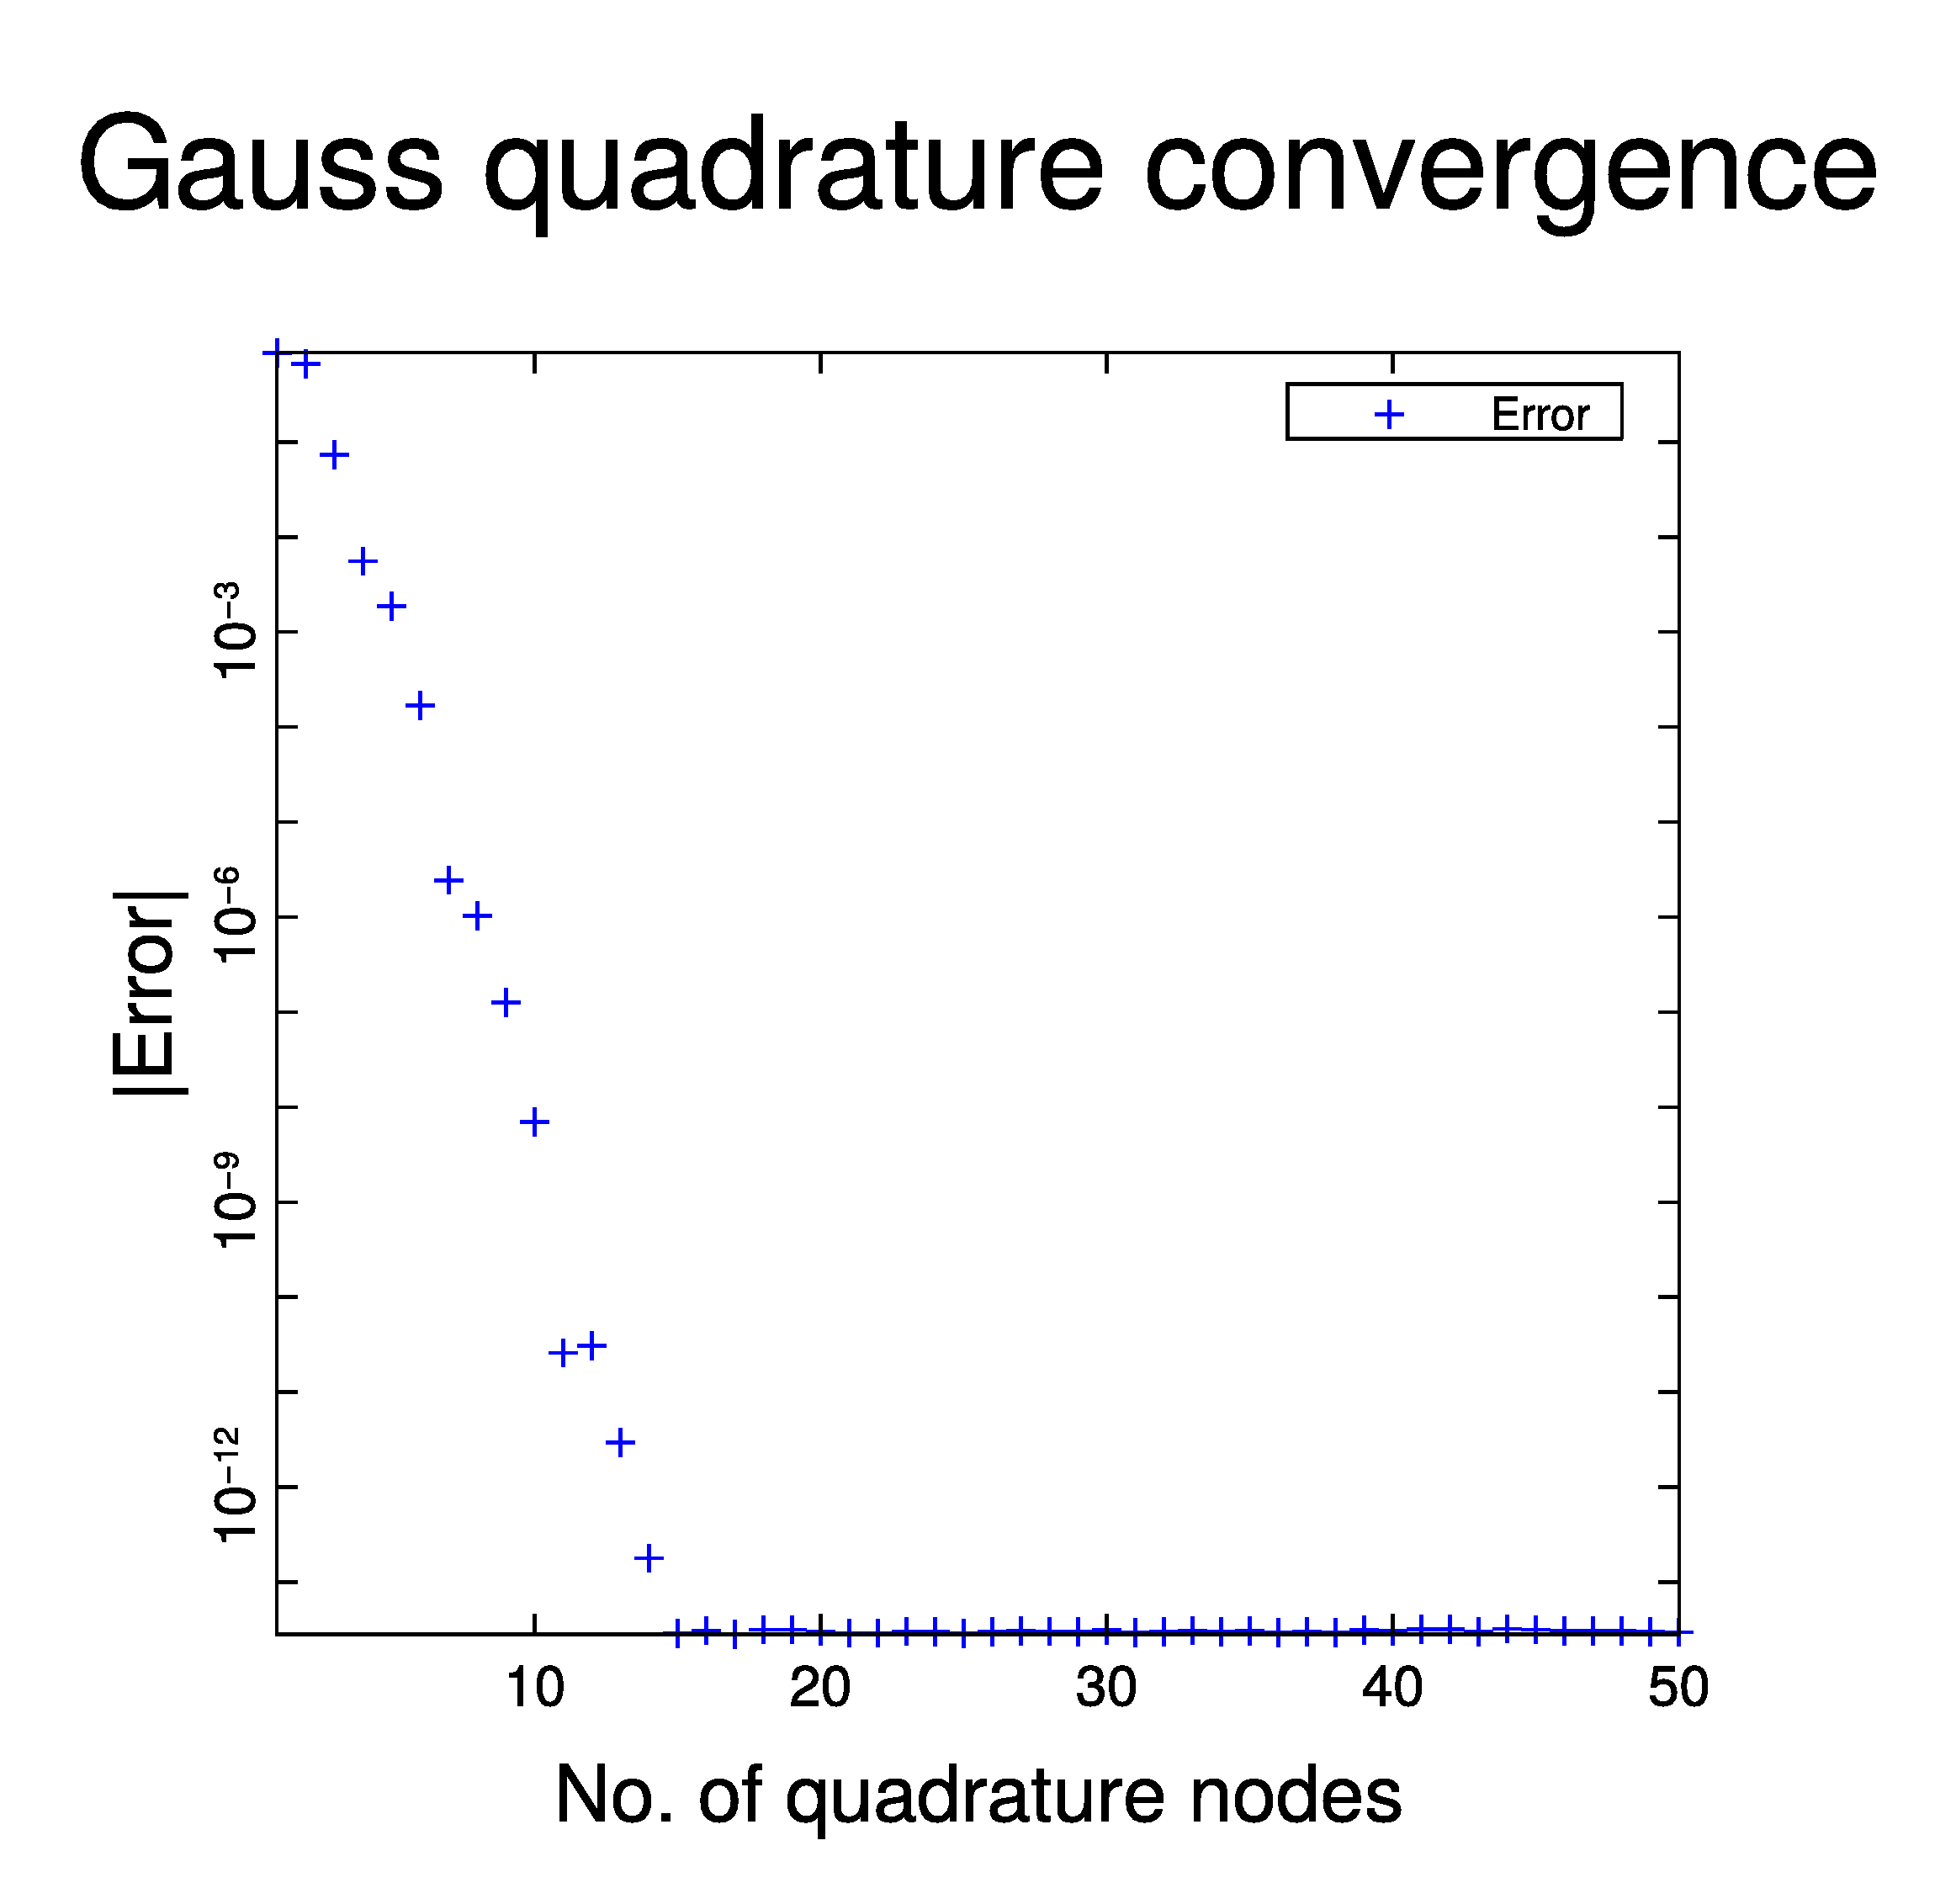
\includegraphics[width=0.6\textwidth]{\problems/ch_numericalquadrature/PICTURES/GaussConvCV.eps}
\caption{Convergence of \texttt{GaussConvCV.m}.}
\label{fig:GaussianQuadrature_GaussConvCV}
\end{figure}
\end{solution}
\end{subproblem}

%%%%%%%%%%%% SUBPROBLEM 5
\begin{subproblem}[3] \label{subprb:GaussianQuadrature_5}
Explain the difference between the results obtained in subtasks \ref{subprb:GaussianQuadrature_1} and \ref{subprb:GaussianQuadrature_4}.

\begin{solution}
The convergence is now exponential.
The integrand of the original integral belongs to $C^0([-1,1])$ but not to $C^1([-1,1])$ because the derivative of the $\arcsin$ function blows up in $\pm1$.
The change of variable provides an analytic integrand: $x\cos(x)\sinh(\sin x)$.
Gauss quadrature ensures exponential convergence only if the integrand is analytic.
This explains the algebraic and the exponential convergence.
\end{solution}
\end{subproblem}

\end{problem}

\begin{problem}[Numerical integration of improper integrals] 

 We want to devise a numerical method for the computation of improper integrals of the form $\int_{-\infty}^{\infty} f(t) dt$ for continuous functions $f: \IR \rightarrow \IR$ that decay sufficiently fast for $\lvert t \rvert \rightarrow \infty$ (such that they are integrable on $\IR$). 
 
 A first option $(T)$ is the truncation of the domain to a bounded interval $[-b,b], b \leq \infty$, that is, we approximate:
 \begin{align*}
  \int_{-\infty}^{\infty} f(t) dt \approx \int_{-b}^{b} f(t) dt
 \end{align*}
 and then use a standard quadrature rule (like Gauss-Legendre quadrature) on $[-b,b]$.
 
 \begin{subproblem}[1]
  For the integrand $g(t) := 1 / (1 + t^2)$ determine $b$ such that the truncation error $E_T$ satisfies:
  \begin{align}
   E_T := \left\lvert  \int_{-\infty}^{\infty} g(t) dt - \int_{-b}^{b} g(t) dt \right \rvert \leq 10^{-6}
  \end{align}
  \begin{solution}
  An antiderivative of $g$ is $\mathrm{atan}$. The function $g$ is even.
  \begin{align}
   E_T = 2 \int_b^\infty g(t) dt = \lim_{x \rightarrow \infty} 2 \mathrm{atan}(x) - 2 \mathrm{atan}(b) = \pi - 2 \mathrm{atan}(b) \overset{!}{<} 10^{-6}
  \end{align}
  i.e. $b > \tan((\pi -10^{-6}) / 2) = \cot(10^{-6} / 2)$.
  \end{solution}
 \end{subproblem}
 
 \begin{subproblem}[1]
  What is the algorithmic difficulty faced in the implementation of the truncation approach for a generic integrand?
  \begin{solution}
   A good choice of $b$ requires a detailed knowledge about the decay of $f$, which may not be available for $f$ defined implicitly.
  \end{solution}
 \end{subproblem}

 A second option $(S)$ is the transformation of the improper integral to a bounded domain by substitution. For instance, we may use the map $t = \cot(s)$.
 
 \begin{subproblem}[2]
  Into which integral does the substitution $t = \cot(s)$ convert $\int_{-\infty}^{\infty} f(t) dt$?
  \begin{solution}
  \begin{align}
   &\frac{dt}{ds} = - (1+\cot^2(s)) = -(1+t^2) \\
   & \int_{-\infty}^{\infty} f(t) dt = - \int_\pi^0 f(\cot(s)) (1+\cot^2(s)) ds = \int_0^\pi \frac{f(\cot(s))}{\sin^2(s)} ds,
  \end{align}
  because $\sin^2(\theta) = \frac{1}{1+\cot^2(\theta)}$.
  \end{solution}
 \end{subproblem}
 
 \begin{subproblem}[1] \label{subprb:transformed_int_f_M}
  Write down the transformed integral explicitly for $g(t) := \frac{1}{1+t^2}$. Simplify the integrand.
  \begin{solution}
  \begin{align}
   \int_0^\pi \frac{1}{1 + \cot^2(s)} \frac{1}{\sin^2(s)} ds = \int_0^\pi \frac{1}{\sin^2(s) + \cos^2(s)} ds = \int_0^\pi ds = \pi
  \end{align}
  \end{solution}
 \end{subproblem}

 \begin{subproblem}[2] \label{subprb:transformed_int_cpp_impl}
  Write a \Cpp{} function:
  \begin{lstlisting}
   template <typename function>
   double quadinf(int n, const function &f);
  \end{lstlisting}
  that uses the transformation from \ref{subprb:transformed_int_f_M} together with $n$-point Gauss-Legendre quadrature to evaluate $\int_{-\infty}^{\infty} f(t) dt$. $f$ passes an object that provides an evaluation operator of the form:
  \begin{lstlisting}
   double operator() (double x) const;
  \end{lstlisting}
  \begin{hint}
   See \verb|quadinf_template.cpp|.
  \end{hint}
  \begin{hint}
   A lambda function with signature
  \begin{lstlisting}
  (double) -> double
  \end{lstlisting}
  automatically satisfies this requirement.
  \end{hint}
\cprotEnv \begin{solution}
   See \verb|quadinf.cpp|.
  \end{solution}
 \end{subproblem}

 \begin{subproblem}[1]
  Study the convergence as $n \rightarrow \infty$ of the quadrature method implemented in \ref{subprb:transformed_int_cpp_impl} for the integrand $h(t) := \exp(-(t-1)^2)$ (shifted Gaussian). What kind of convergence do you observe?
  \begin{hint}
  \begin{align}
   \int_{-\infty}^{\infty} h(t) dt = \sqrt{\pi}
  \end{align}
  \end{hint}
\cprotEnv \begin{solution}
   We observe exponential convergence. See \verb|quadinf.cpp|.
  \end{solution}
 \end{subproblem}

\end{problem}
 
% ncse_new/p2_InterpolationApproximation/ch4_NumericalQuadrature/ex_QuadraturePlots.tex
% exercise requires:   ExQuadPlots.jpg     ExQuadPlots.eps
% solutions require:   -

\begin{problem}[Quadrature plots] \label{prb:QuadraturePlots}

We consider three different functions on the interval $I=[0,1]$:
\begin{align*}
\text{function A:}\quad f_A&\in \text{analytic}\;,\quad f_A\notin\Cp_k\; \forall\;k\in\IN\;;\\
\text{function B:}\quad f_B&\in C^0(I)\;,\quad f_B\notin C^1(I)\;;\\
\text{function C:}\quad f_C&\in\Cp_{12}\;,
\end{align*}
where $\Cp_k$ is the space of the polynomials of degree at most $k$ defined on $I$.
The following quadrature rules are applied to these functions:
\begin{itemize}
\item quadrature rule A,\quad global Gauss quadrature;
\item quadrature rule B,\quad composite trapezoidal rule;
\item quadrature rule C,\quad composite 2-point Gauss quadrature.
\end{itemize}
The corresponding absolute values of the quadrature errors are plotted against the number of function evaluations in Figure~\ref{fig:QuadraturePlots}.
Notice that only the quadrature errors obtained with an even number of function evaluations are shown.

\begin{figure}[hbt]
\hspace{8mm}
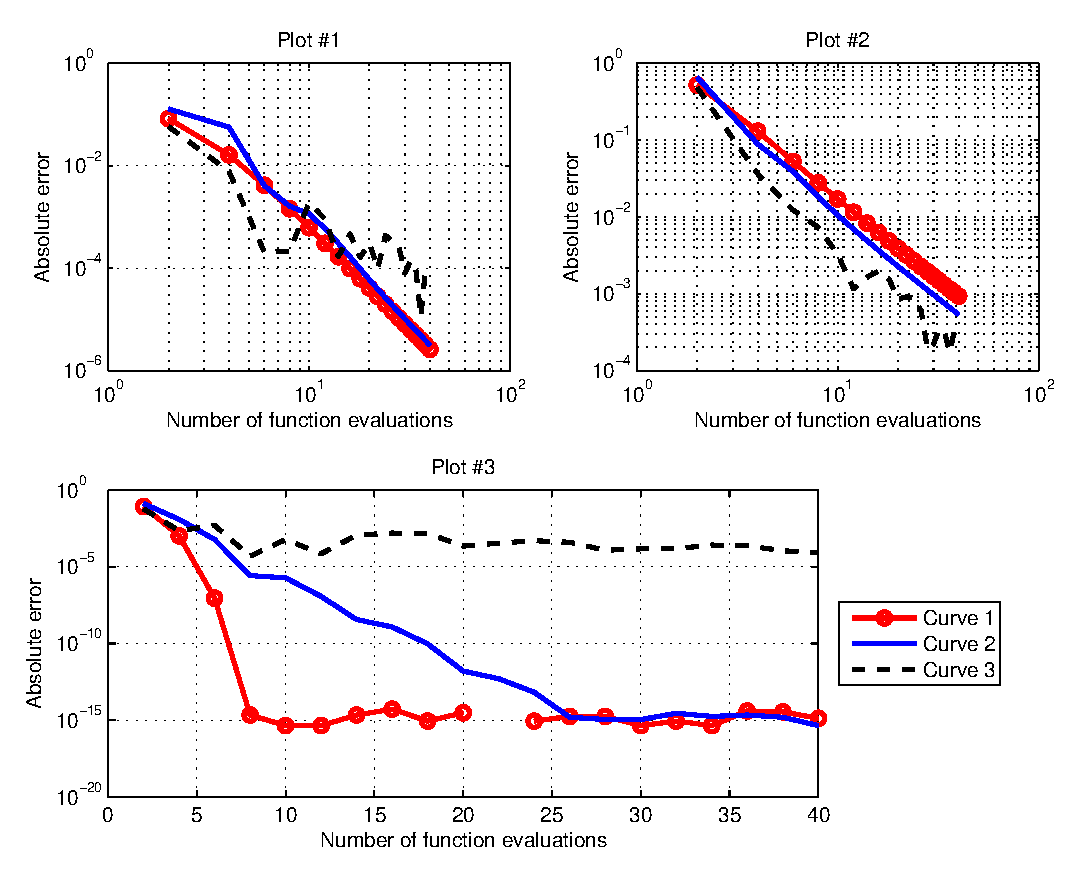
\includegraphics[width=0.9\textwidth]{\problems/ch_numericalquadrature/PICTURES/ExQuadPlots.eps}
\caption{Quadrature convergence plots for different functions and different rules.}
\label{fig:QuadraturePlots}
\end{figure}

%%%%%%%%%%%% SUBPROBLEM 1

\begin{subproblem}[3] \label{prb:QuadraturePlots_1}
Match the three plots (plot \#1, \#2 and \#3) with the three quadrature rules (quadrature rule A, B, and  C). Justify your answer.\\[1.5ex]
\begin{hint}
Notice the different axis scales in the plots.
\end{hint}

\begin{solution}
Plot \#1 --- Quadrature rule C, Composite 2-point Gauss:\\
algebraic convergence for every function, about $4^{th}$ order for two functions.

Plot \#2 --- Quadrature rule B, Composite trapezoidal:\\ algebraic convergence for every function, about $2^{nd}$ order.

Plot \#3 --- Quadrature rule A, Global Gauss:\\ algebraic convergence for one function, exponential for another one, exact integration with 8 evaluations for the third one.
\end{solution}
\end{subproblem}

%%%%%%%%%%%% SUBPROBLEM 2

\begin{subproblem}[3] \label{prb:QuadraturePlots_2}
The quadrature error curves for a particular function $f_A$, $f_B$ and $f_C$ are plotted in the same style (curve 1 as red line with small circles, curve 2 means the blue solid line, curve 3 is the black dashed line).
Which curve corresponds to which function ($f_A$, $f_B$, $f_C$)?
Justify your answer.

\begin{solution}
Curve 1 red line and small circles --- $f_C$ polynomial of degree 12:\\
integrated exactly with 8 evaluations with global Gauss quadrature.

Curve 2 blue continuous line only --- $f_A$ analytic function:\\
exponential convergence with global Gauss quadrature.

Curve 3 black dashed line --- $f_B$ non smooth function:\\
algebraic convergence with global Gauss quadrature.
\end{solution}
\end{subproblem}
\end{problem}

\end{sheet}

%%% PS11
\begin{sheet}{11}{26.11.2015}{03.12.2015}

\begin{problem}[Efficient quadrature of singular integrands \coreproblem]
\label{prb:effquadsing}
 
 This problem deals with efficient numerical quadrature of non-smooth integrands with a special structure. Before you tackle this problem, read about regularization of integrands by transformation \ncserem{rem:sqrtquad}.

 Our task is to develop quadrature formulas for integrals of the form:
 \begin{align} \label{eq:effquadsingint}
  W(f) := \int_{-1}^1 \sqrt{1 - t^2}\, f(t) dt,
 \end{align}
 where $f$ possesses an analytic extension to a complex neighbourhood of $[-1,1]$.

 \begin{subproblem}[1]
 The provided function
 \begin{lstlisting}[language=c++]
  QuadRule gauleg(unsigned int n);
 \end{lstlisting}
 returns a structure \verb|QuadRule| containing nodes $(x_j)$ and weights $(w_j)$
 of a Gauss-Legendre quadrature ($\to$ \lref{def:gaussquad}) on $[-1,1]$ with $n$
 nodes. Have a look at the file \verb|gauleg.hpp| and \verb|gauleg.cpp|, and
 understand how the implementation works and how to use it.
 
  \cprotEnv \begin{hint}
   Learn/remember how linking works in \Cpp{}. To use the function \verb|gauleg| (declared in \verb|gauleg.hpp| and defined in \verb|gauleg.cpp|) in a file \verb|file.cpp|, first \verb|include| the header file \verb|gauleg.hpp| in the file \verb|file.cpp|, and then compile and link the files \verb|gauleg.cpp| and \verb|file.cpp|. Using \verb|gcc|:
   \begin{lstlisting}
g++ [compiler opts.] -c gauleg.cpp
g++ [compiler opts.] -c file.cpp
g++ [compiler opts.]  gauleg.o file.o -o exec_name
   \end{lstlisting}
   If you want to use \verb|CMake|, have a look at the file \verb|CMakeLists.txt|.
  \end{hint}
  
  \cprotEnv \begin{solution}
   See documentation in \verb|gauleg.hpp| and \verb|gauleg.cpp|.
  \end{solution}
 \end{subproblem}

 \begin{subproblem}[1]
   Study \lref{par:quadbest} in order to learn about the convergence of
   Gauss-Legendre quadrature. 
 \end{subproblem}

 \begin{subproblem}[3] \label{subprb:effquadsingint}
  Based on the function \verb|gauleg|, implement a \Cpp{} function
 \begin{lstlisting}[language=c++]
 template <class func>
 double quadsingint(func&& f, unsigned int n);
 \end{lstlisting}
 that approximately evaluates \eqref{eq:effquadsingint} using $2n$ evaluations of $f$. An object of type \verb|func| must provide an evaluation operator
 \begin{lstlisting}[language=c++]
 double operator(double t) const;
 \end{lstlisting}
 For the quadrature error asymptotic exponential convergence to zero for
 $n \rightarrow \infty$ must be ensured by your function.
 
 
 \begin{hint}
  A \Cpp{} lambda function provides such operator.
 \end{hint}
 
 \begin{hint}
   You may use the classical binomial formula
   $\sqrt{1 - t^2} = \sqrt{ 1 - t} \sqrt{1 + t}$.
 \end{hint}
 
  \cprotEnv \begin{hint}
  You can use the template \verb|quadsingint_template.cpp|.
  \end{hint}

  \cprotEnv \begin{solution}
   Exploiting the hint, we see that the integrand is non-smooth in $\pm 1$. 
   
   The first possible solution is the following (I): we split the integration domain $[-1,1]$ in $[0,1]$ and $[-1,0]$. Applying the substitution $s = \sqrt{1 \pm t}$ (sign depending on which part of the integrals considered), $t = \pm(s^2 - 1)$:
   \begin{align*}
    \frac{dt}{ds} = \pm2s \\
    W(f) := \int_{-1}^1 \sqrt{1 - t^2} f(t) dt = \int_{-1}^0 \sqrt{1 - t^2} f(t) dt + \int_0^1 \sqrt{1 - t^2} f(t) dt \\
    = \int_0^{1} 2 \cdot s^2 \sqrt{2 - s^2} f(-s^2+1) ds + \int_0^{1} 2 \cdot s^2 \sqrt{2 - s^2} f(s^2-1) ds.
   \end{align*}
   Notice how the resulting integrand is analytic in a neighbourhood of the domain
   of integration because, for instant, {$t\mapsto \sqrt{1+t}$} is analytic
   in a neighborhood of $[0,1]$. 
   
   Alternatively (II), one may use the trigonometric substitution $t = \sin s$, with $\frac{dt}{ds} = \cos s$ obtaining
   \begin{align*}
    W(f) & := \int_{-1}^1 \sqrt{1 - t^2} f(t) dt \\
    & = \int_{-\pi / 2}^{\pi / 2} \sqrt{1 - \sin^2\! s}\, f(\sin s) \cos s\,ds = \int_{-\pi / 2}^{\pi / 2} \cos^2\! s \, f(\sin s) ds.
   \end{align*}
   This integrand is also analytic.
%    hence, using $r = \sqrt{\sqrt(2) - s}, s = \sqrt{2} - r^2$:
%    \begin{align*}
%     \frac{ds}{dr} = -2r \\
%     W(f) := \int_0^{\sqrt{2}} 2 \cdot s^2 \sqrt{2 - s^2} f(1 - s^2) ds  = \int_0^{\sqrt{\sqrt{2}}} 4 r^2 \sqrt{2 \sqrt{2}-r^2} (\sqrt{2} - r^2)^2 f(1 - (\sqrt{2} - r^2)^2) dr
%    \end{align*}
   The \Cpp{} implementation is in \verb|quadsingint.cpp|.
  \end{solution}

 \end{subproblem}

 \begin{subproblem}[2]
  Give formulas for the nodes $c_j$ and weights $\tilde{w}_j$ of a $2n$-point quadrature rule on $[-1,1]$, whose application to the integrand $f$ will produce the same results as the function \verb|quadsingint| that you implemented in \ref{subprb:effquadsingint}.
  
  \cprotEnv \begin{solution}
   Using substitution (I). Let $(x_j, w_j)$, $j=1,\dots,n$ be the Gauss nodes and weights relative to the Gauss quadrature of order $n$ in the interval $[0,1]$. The nodes are mapped from $x_j$ in $[0,1]$ to $c_l$ for $l \in 1,\dots,2n$ in $[-1,1]$ as follows:
    \begin{align*}
     c_{2j-i}  = (-1)^i (1-x_j^2),\qquad j=1,\dots,n,\;i=0,1.  
      \end{align*}
    The weights $\tilde{w}_{l}, l = 1,\dots,2n$, become:
    \begin{align*}
     \tilde{w}_{2j-i} = 2 w_j x_j^2 \sqrt{2 - x_j^2},\qquad j=1,\dots,n,\;i=0,1.
    \end{align*}
    
   Using substitution (II). Let $(x_j, w_j)$, $j=1,\dots,n$ be the Gauss nodes and weights relative to the Gauss quadrature of order $n$ in the interval $[-1,1]$.  The nodes are mapped from $x_j$ to $c_j$  as follows:
    \begin{align*}
     c_j = \sin(x_j  \pi / 2),\qquad j=1,\dots,n
    \end{align*}
    The weights $\tilde{w}_{j}, j = 1,\dots,n$, become:
    \begin{align*}
     \tilde{w}_{j} = w_j \cos^2(x_j  \pi / 2) \pi / 2.
    \end{align*}
  \end{solution}

 \end{subproblem}

%  \begin{subproblem}[4]
%   What is the maximal degree of polynomials $f$, for which \verb|quadsingint|, in absence of round-off, will return the exact value of \eqref{eq:effquadsingint}?
%   
%    \begin{solution}
%     
%    \end{solution}
%  \end{subproblem}
 
 \begin{subproblem}[1]
  Tabulate the quadrature error:
   \begin{align*}
    \lvert W(f) - \texttt{quadsingint(f,n)} \rvert
   \end{align*}
   for $f(t) := \frac{1}{2+\exp(3t)}$ and $n = 1,2,...,25$. Estimate the $0 < q <
   1$ in the decay law of exponential convergence, see \lref{def:cvgtype}. 

  \cprotEnv   \begin{solution}
   The convergence is exponential with both methods. The \Cpp{} implementation is in \verb|quadsingint.cpp|.
   \end{solution}

 \end{subproblem}

 
\end{problem}


\begin{problem}[Nested numerical quadrature]
 
 A laser beam has intensity
 \begin{align*}
  I(x,y) = \exp(- \alpha ((x-p)^2 + (y-q)^2) )
 \end{align*}
 on the plane orthogonal to the direction of the beam.
 
 \begin{subproblem}[1] \label{subprb:nested_quad_1}
  Write down the radiant power absorbed by the triangle
  \begin{align*}
   \bigtriangleup := \{(x,y)^T \in \IR^2 \; | \; x \geq 0, y \geq 0, x+y \leq 1 \}
  \end{align*}
  as a double integral.
  
  \begin{hint}
   The  radiant power absorbed by a surface is the integral of the intensity over the surface.
  \end{hint}
  
  \begin{solution}
   The radiant power absorbed by $\bigtriangleup$ can be written as:
   \begin{align*}
    \int_\bigtriangleup I(x,y) dx dy = \int_0^1 \int_0^{1-y} I(x,y) dx dy.
   \end{align*}
  \end{solution}
 \end{subproblem}

 \begin{subproblem}[3] \label{subprb:nested_quad_2}
  Write a \Cpp{} function 
  \begin{lstlisting}[language=c++]
template <class func>
double evalgaussquad(double a, double b, func&& f, const QuadRule & Q);
  \end{lstlisting}
  that evaluates an the $N$-point quadrature for an integrand passed in \texttt{f}
  in $[a,b]$. It should rely on the quadrature rule on the reference interval
  $[-1,1]$ that supplied through an object of type \texttt{QuadRule}. 
  (The vectors \verb|weights| and \verb|nodes| denote the weights and
  nodes of the reference quadrature rule respectively.)
  
  \begin{hint}
   Use the function \verb|gauleg| declared in \verb|gauleg.hpp| 
   and defined in \verb|gauleg.cpp| to compute nodes and weights in $[-1,1]$.
   See \ref{prb:effquadsing} for further explanations. 
  \end{hint}
  
  \begin{hint}
  You can use the template \verb|laserquad_template.cpp|.
  \end{hint}
  
  \cprotEnv \begin{solution}
   See \verb|laserquad.cpp| and \verb|CMakeLists.txt|.
  \end{solution}
 \end{subproblem}

 \begin{subproblem}[4] \label{subprb:nested_quad_3}
  Write a \Cpp{} function
  \begin{lstlisting}[language=c++]
template <class func>
double gaussquadtriangle(func&& f, int N)
  \end{lstlisting}
  for the computation of the integral
  \begin{align} \label{eq:subprb_nested_quad_2}
   \int_\bigtriangleup f(x,y) dx dy,
  \end{align}
  using nested $N$-point, 1D Gauss quadratures (using the functions \verb|evalgaussquad| of \ref{subprb:nested_quad_2} and  \verb|gauleg|).
  
  \begin{hint}
   Write \eqref{eq:subprb_nested_quad_2} explicitly as a double integral. Take particular care to correctly find the intervals of integration.
  \end{hint}
  
  \begin{hint}
   Lambda functions of \Cpp{} are well suited for this kind of implementation.
  \end{hint}

  
  \cprotEnv \begin{solution}
   The integral can be written as
   \begin{align*}
    \int_\bigtriangleup f(x,y) dx dy = \int_0^1 \int_0^{1-y} f(x,y) dx dy.
   \end{align*}
   In the \Cpp{} implementation, we define the auxiliary (lambda) function $f_y$:
   \begin{align*}
    \forall y \in [0,1], f_y: [1,1-y] \rightarrow \IR, x \mapsto f_y(x) := f(x,y)
   \end{align*}
   We also define the (lambda) approximated integrand:
   \begin{align}
    g(y) := \int_0^{1-y} f_y(x) dx \approx \frac{1}{1-y} \sum_{i = 0}^N w_i f_y\left(\frac{x_i + 1}{2}  (1-y)\right) =: \mathcal{I}(y),
   \end{align}
   the integral of which can be approximated, using a nested Gauss quadrature:
   \begin{align}
    \int_\bigtriangleup f(x,y) dx dy  = \int_0^1  \int_0^{1-y} f_y(x) dx dx = \int_0^1 g(y) dy \approx \frac{1}{2} \sum_{j = 1}^N w_j \mathcal{I}\left(\frac{y_j + 1}{2}\right).
   \end{align}
   The implementation can be found in \verb|laserquad.cpp|.
  \end{solution}

 \end{subproblem}

 \begin{subproblem}[1]
  Apply the function \verb|gaussquadtriangle| of \ref{subprb:nested_quad_3} to the subproblem \ref{subprb:nested_quad_1} using the parameter $\alpha = 1, p = 0, q = 0$. Compute the error w.r.t to the number of nodes $N$. What kind of convergence do you observe? Explain the result.
  
  \begin{hint}
   Use the ``exact'' value of the integral $0.366046550000405$.
  \end{hint}
  
  \cprotEnv \begin{solution}
  As one expects from theoretical considerations, the convergence is exponential. The implementation can be found in \verb|laserquad.cpp|.
  \end{solution}


 \end{subproblem}

 
\end{problem}

\begin{problem}[Weighted Gauss quadrature]
The development of an alternative quadrature formula for \eqref{eq:effquadsingint} relies on the Chebyshev polynomials of the second kind $U_n$, defined as
\begin{equation*}
U_n(t)=\frac{\sin((n+1)\arccos t)}{\sin(\arccos t)}, \qquad n\in\n.
\end{equation*}
Recall the role of the orthogonal Legendre polynomials in the derivation and definition of Gauss-Legendre quadrature rules (see \lref{par:LP}).

As regards the integral \eqref{eq:effquadsingint}, this role is played by the $U_n$, which are orthogonal polynomials with respect to a weighted $L^2$ inner product, see \lref{eq:wSPLtwo}, with weight given by $w(\tau)=\sqrt{1-\tau^2}$.
% SUBPROBLEM 1
\begin{subproblem}[2]
Show that the $U_n$ satisfy the 3-term recursion
\[
U_{n+1}(t)=2tU_n(t)-U_{n-1}(t),\qquad U_0(t)=1,\qquad U_1(t)=2t,
\]
for every $n\ge 1$.
\begin{solution}
The case $n=0$ is trivial, since $U_0(t)=\frac{\sin(\arccos t)}{\sin(\arccos t)}=1$, as desired. Using the trigonometric identity $\sin 2x = \sin x \cos x$, we have $U_1(t)=\frac{2\sin(\arccos t)}{\sin(\arccos t)}=2\cos \arccos t = 2t$, as desired. Finally, using the identity $\sin (x+y) = \sin x \cos y + \sin y \cos x$, we obtain for $n\ge 2$
\[
\begin{split}
U_{n+1}(t)   &= \frac{\sin((n+1)\arccos t)t + \cos((n+1)\arccos t) \sin (\arccos t)}{\sin(\arccos t)} \\
& = U_n(t) t+\cos((n+1)\arccos t).
\end{split}
\]
Similarly, we have
\[
\begin{split}
U_{n-1}(t)&=\frac{\sin((n+1 -1 )\arccos t)}{\sin(\arccos t)} \\ 
&= \frac{\sin((n+1)\arccos t)t - \cos((n+1)\arccos t) \sin (\arccos t)}{\sin(\arccos t)}\\
& = U_n(t) t-\cos((n+1)\arccos t).
\end{split}
\]
Combining the last two equalities we obtain the desired 3-term recursion.
\end{solution}
\end{subproblem}

% SUBPROBLEM 2
\begin{subproblem}[1]
Show that $U_n\in \Pol{n}$ with leading coefficient $2^n$.
\begin{solution}
Let us prove the claim by induction. The case $n=0$ is trivial, since $U_0(t)=1$. Let us now assume that the statement is true for every $k=0,\dots,n$ and let us prove it for $n+1$. In view of $U_{n+1}(t)=2tU_n(t)-U_{n-1}(t)$, since by inductive hypothesis $U_n\in\Pol{n}$ and $U_{n-1}\in\Pol{n-1}$, we have that $U_{n+1}\in \Pol{{n+1}}$. Moreover, the leading coefficient will be $2$ times the leading order coefficient of $U_n$, namely $2^{n+1}$, as desired.
\end{solution}
\end{subproblem}

% SUBPROBLEM 3
\begin{subproblem}[2]\label{subpb:orthogonal}
Show that for every $m,n\in\n_0$ we have
\[
\int_{-1}^1 \sqrt{1-t^2}\,U_m(t) U_n(t)\,dt=\frac{\pi}{2}\delta_{mn}.
\]
\begin{solution}
With the substitution $t=\cos s$ we obtain
\[
\begin{split}
\int_{-1}^1 \sqrt{1-t^2}U_m(t) U_n(t)\,dt &= \int_{-1}^1 \sqrt{1-t^2}  \frac{\sin((m+1)\arccos t)\sin((n+1)\arccos t)}{\sin^2(\arccos t)}\,dt \\
&=  \int_{0}^\pi \sin s  \frac{\sin((m+1)s)\sin((n+1)s)}{\sin^2 s}\sin s\,ds \\
&=  \int_{0}^\pi  \sin((m+1)s)\sin((n+1)s)\,ds \\
&=\frac{1}{2} \int_{0}^\pi  \cos((m-n)s) - \cos((m+n+2)s)\,ds. \\
\end{split}
\]
The claim immediately follows, as it was done in \ref{PS9}, \ref{prob:ChebPolyProp}.
\end{solution}
\end{subproblem}

% SUBPROBLEM 4
\begin{subproblem}[1]
What are the zeros $\xi^n_j$ ($j=1,\dots,n$) of $U_n$, $n\ge 1$? Give an explicit formula similar to the formula for the Chebyshev nodes in $[-1,1]$.
\begin{solution}
From the definition of $U_n$ we immediately find that the zeros are given by
\begin{equation}\label{eq:zeros}
\xi^n_j= \cos\left(\frac{j}{n+1}\pi\right),\qquad j=1,\dots,n.
\end{equation}
\end{solution}
\end{subproblem}

% SUBPROBLEM 5
\begin{subproblem}[4]
Show that the choice of weights
\begin{equation*}
w_j=\frac{\pi}{n+1}\sin^2\left(\frac{j}{n+1}\pi\right),\qquad j=1,\dots, n,
\end{equation*}
ensures that the quadrature formula
\begin{equation}\label{eq:quadrature_formula}
Q^U_n(f)=\sum_{j=1}^n w_j f(\xi^n_j)
\end{equation}
provides the exact value of  \eqref{eq:effquadsingint} for $f\in\Pol{n-1}$ (assuming exact arithmetic).
 \begin{hint}
Use  all the previous subproblems.
\end{hint}
\begin{solution}
Since $U_{k}$ is a polynomial of degree exactly $k$, the set $\{U_k:k=0,\dots,n-1\}$ is a basis of $\Pol{n-1}$. Therefore, by linearity it suffices to prove the above identity for $f=U_k$ for every $k$. Fix $k=0,\dots,n-1$. Setting $x=\pi/(n+1)$, from \eqref{eq:zeros} we readily derive
\[
\begin{split}
\sum_{j=1}^n w_j U_k(\xi^n_j) &=  \sum_{j=1}^n \frac{\pi}{n+1}\sin^2\left(\frac{j}{n+1}\pi\right) \frac{\sin((k+1)\arccos \xi^n_j)}{\sin(\arccos \xi^n_j)}\\
&=  x \sum_{j=1}^n \sin(jx) \sin((k+1)jx)\\
&=  \frac{x}{2} \sum_{j=1}^n\left(\cos((k+1-1)jx)-\cos((k+1+1)jx)\right)\\
&=  \frac{x}{2}\Re \sum_{j=0}^n \left( e^{i k x j}-e^{i(k+2) x j}\right)\\
&=  \frac{x}{2}\Re\left( \sum_{j=0}^n  e^{i k x j}-\frac{1-e^{i\pi(k+2)}}{1-e^{i (k+2) x }}\right).
\end{split}
\]
Thus, for $k=0$ we have
\[
\sum_{j=1}^n w_j U_0(\xi^n_j) = \frac{x}{2}\Re\left( \sum_{j=0}^n  1-\frac{1-e^{2\pi i}}{1-e^{ 2 x i }}\right)
= \frac{x}{2}\Re\left( (n+1)-0\right) = \frac{\pi}{2}.
\]

On the other hand, if $k=1,\dots,n-1$ we obtain
\[
\sum_{j=1}^n w_j U_k(\xi^n_j) =  \frac{x}{2}\Re\left( \frac{1-e^{i\pi k}}{1-e^{i k x}}-\frac{1-e^{i\pi(k+2)}}{1-e^{i (k+2) x }}\right) =  \frac{(1-(-1)^k)x}{2}\Re\left( \frac{1}{1-e^{i k x}}-\frac{1}{1-e^{i (k+2) x}}\right).
\]
In view of the elementary equality $(a+ib)(a-ib)=a^2+b^2$ we have $\Re(1/(a+ib)) = a/(a^2+b^2)$. Thus
\[
\Re\left( \frac{1}{1-e^{i k x}}\right) = \Re\left( \frac{1}{1-\cos(kx)-i\sin(kx)} \right)= \frac{1-\cos(kx)}{(1-\cos(kx))^2 + \sin(kx)^2}  = \frac{1}{2}.
\]
Arguing in a similar way we have $\Re\,(1-e^{i (k+2) x})^{-1}= 1/2$. Therefore for $k=1,\dots,n-1$ we have
\[
\sum_{j=1}^n w_j U_k(\xi^n_j) = \frac{(1-(-1)^k)x}{2}\left( \frac{1}{2} -\frac{1}{2} \right) = 0.
\]
To summarise, we have proved that
\[
 \sum_{j=1}^n w_j U_k(\xi^n_j) = \frac{\pi}{2}\delta_{k0},\qquad k=0,\dots,n-1.
  \]
  
Finally, the claim follows from \ref{subpb:orthogonal}, since $U_0(t)=1$ and so the integral in  \eqref{eq:effquadsingint} is nothing else than the weighted scalar product between $U_k$ and $U_0$.
\end{solution}
\end{subproblem}

% SUBPROBLEM 6
\begin{subproblem}[2]
Show that the quadrature formula \eqref{eq:quadrature_formula} gives the exact value of \eqref{eq:effquadsingint}  even for every $f\in \Pol{2n-1}$.
 \begin{hint}
See \lref{thm:Gaussquad}.
\end{hint}
\begin{solution}
The conclusion follows by applying the same argument given in  \lref{thm:Gaussquad} with the weighted $L^2$ scalar product with weight $w$ defined above.
\end{solution}
\end{subproblem}

% SUBPROBLEM 7
\begin{subproblem}[3]
Show that the quadrature error
\[
|Q^U_n(f)-W(f)|
\]
decays to $0$ exponentially as $n\to \infty$ for every $f\in C^\infty([-1,1])$ that admits an analytic extension to an open subset of the complex plane.
\begin{hint}
See \lref{par:quadbest}.
\end{hint}
\begin{solution}
By definition, the weights defined above are positive, and the quadrature rule is exact for polynomials up to order $2n-1$. Therefore, arguing as in \lref{par:quadbest}, we obtain the exponential decay, as desired.
\end{solution}
\end{subproblem}

% SUBPROBLEM 8
\begin{subproblem}[2]
Write a \Cpp{} function
\begin{lstlisting}
template<typename Function>
double quadU(const Function &f, unsigned int n)
\end{lstlisting}
that gives $Q^U_n(f)$ as output, where \texttt{f} is an object with an evaluation operator, like a lambda function, representing $f$, e.g.
\begin{lstlisting}
auto f = [] (double & t) {return 1/(2 + exp(3*t));};
\end{lstlisting}
\begin{solution}
See file \texttt{quadU.cpp}.
\end{solution}
\end{subproblem}


% SUBPROBLEM 8
\begin{subproblem}[2]
Test your implementation with the function $f(t)=1/(2+e^{3t})$ and
$n=1,\dots,25$. Tabulate the quadrature error $E_n(f)=|W(f)-Q^U_n(f)|$ using the
``exact'' value $W(f)=0.483296828976607$. Estimate the parameter $0\le q<1$ in the
asymptotic decay law $E_n(f)\approx Cq^n$ characterizing (sharp) exponential
convergence, see \lref{def:cvgtype}. 
\begin{solution}
See file \texttt{quadU.cpp}.  An approximation of $q$ is given by $E_n(f)/E_{n-1}(f)$.
\end{solution}
\end{subproblem}


\end{problem}
\begin{problem}[Generalize ``Hermite-type'' quadrature formula]
 
 \begin{subproblem}[4]
 Determine $A,B,C, x_1 \in \IR$ such that the quadrature formula:
 \begin{align} \label{eq:gen_hermite_quad}
  \int_0^1 f(x) dx \approx A f(0) + B f'(0) + C f(x_1)
 \end{align}
 is exact for polynomials of highest possible degree.
 
 \cprotEnv \begin{solution}
  The quadrature is exact for every polynomial $p(x) \in \mathcal{P}^n$, if and only if it is exact for $1,x,x^2,\dots,x^n$. If we apply the quadrature to the first monomials:
  \begin{align}
   1 = \int_0^1 1 dx & = A \cdot 1 + B \cdot 0 + C \cdot 1 = A + C\\
   \frac{1}{2} = \int_0^1 x dx & = A \cdot 0 + B \cdot 1 + C \cdot x_1 = B + C x_1 \\
   \frac{1}{3} = \int_0^1 x^2 dx & = A \cdot 0 + B \cdot 0 + C \cdot x_1^2 = C x_1^2 \\
   \frac{1}{4} = \int_0^1 x^3 dx & = A \cdot 0 + B \cdot 0 + C \cdot x_1^3 = C x_1^3
  \end{align}
  $\Rightarrow B = \frac{1}{2} - C x_1, C = \frac{1}{3 x_1^2} \Rightarrow \frac{1}{4} = \frac{1}{3 x_1^2} x_1^3 = \frac{1}{3} x_1, A = \frac{11}{27}$, i.e.
  \begin{align}
  x_1 = \frac{3}{4}, C = \frac{16}{27}, B = \frac{1}{18}, A = \frac{11}{27}.
  \end{align}
  Then
  \begin{align}
   \frac{1}{5} = \int_0^1 x^4 dx \neq A \cdot 0 + B \cdot 0 + C \cdot x_1^4 = C \cdot x_1^4 = \frac{16}{27} \frac{81}{256}.
  \end{align}
  Hence, the quadrature is exact for polynomials up to degree $3$.
 \end{solution}
 
 \end{subproblem}
 
 \begin{subproblem}[4]
 
 Compute an approximation of $z(2)$, where the function $z$ is defined as the solution of the initial value problem
 \begin{align}
  z'(t) = \frac{t}{1 + t^2}\quad,\quad z(1) = 1\;.
 \end{align}
 
 \cprotEnv \begin{solution}
  We know that
 \begin{align}
  z(2) - z(1) = \int_1^2 z'(x) dx,
 \end{align}
 hence, applying \eqref{eq:gen_hermite_quad} and the transformation $x \mapsto x + 1$, we obtain:
 \begin{align}
  z(2) = \int_0^1 z'(x + 1) dx + z(1) \approx \frac{11}{27} \cdot z'(1) + \frac{1}{18} \cdot z''(1) + \frac{16}{27} \cdot z'\left(\frac{7}{4}\right) + z(1).
 \end{align}
  With $z''(x) = - \frac{2 \cdot x}{(1 + x^2)^2}$ and:
 \begin{align*}
  z(1) = 1, \\
  z'(1) = \frac{1}{1 + 1^2} = \frac{1}{2}, \\
  z''(1) = - \frac{2 \cdot 1}{(1 + 1^2)^2} = -\frac{1}{2}, \\
  z'\left(\frac{7}{4}\right) = \frac{(\frac{7}{4})}{1 + (\frac{7}{4})^2} = \frac{28}{65},
 \end{align*}
  we obtain
  \begin{align*}
   z(2) = \int_0^1 z'(x + 1) dx + z(1) \approx \frac{11}{27} \cdot \frac{1}{2} - \frac{1}{18} \cdot \frac{1}{2} + \frac{16}{27} \cdot \frac{28}{65} + 1 = 1.43 \dots
  \end{align*}
  For sake of completeness, using the antiderivative of $z'$:
  \begin{align*}
   z(2) = \int_1^2 z'(x) dx + z(1) = \frac{1}{2} \log(x^2 + 1) |_1^2 + 1 = 1.45 \dots
  \end{align*}
 \end{solution}
 
 \end{subproblem}
 
\end{problem}

\end{sheet}

%%% PS12
\begin{sheet}{12}{03.12.2015}{10.12.2015}\label{PS12}
% ncse_new/p3_ODE/ch1_SingleStepMethods/ex_RK3.tex
% it contains part of the solution of ex_TaylorODE, 2 methods for the same problem
% last year it was called Heun
% solution:           ExRK3solution.eps   ExRK3convergence.eps   RK3_step.m     MyIntegrate.m   pred_prey.m       exRK3.m

\begin{problem}[Three-stage Runge-Kutta method \coreproblem] \label{prb:RK3}
The most widely used class of numerical integratos for IVPs is that of \emph{explicit} Runge-Kutta (RK) methods as defined in \ncsedef{def:rk}. They are usually described by giving their coefficients in the form of a Butcher scheme \ncseref{eq:BSexpl}.

\begin{subproblem}[4] \label{subprb:RK3_1}
Implement a header-only \Cpp{} class \verb|RKIntegrator|
\begin{lstlisting}[language=c++]
template <class State>
class RKIntegrator {
public:
  RKIntegrator(const Eigen::MatrixXd & A,
               const Eigen::VectorXd & b) {
    // TODO: given a Butcher scheme in A,b, initialize RK method for solution of an IVP
  }

  template <class Function>
  std::vector<State> solve(const Function &f, double T,
                           const State & y0,
                           unsigned int N) const {
    // TODO: computes N uniform time steps for the ODE y'(t) = f(y) up to time T of RK method with initial value y0 and store all steps (y_k) into return vector 
  }
private:
  template <class Function>
  void step(const Function &f, double h,
            const State & y0, State & y1) const {
    // TODO: performs a single step from y0 to y1 with step size h of the RK method for the IVP with rhs f
  }

  // TODO: hold data for RK methods
};
\end{lstlisting}
which implements a generic RK method given by a Butcher scheme to solve the autonomous initial value problem $\dot{\Vy} = \Vf(\Vy)$, $\Vy(t_{0}) = \Vy_{0}$.
    
\begin{hint}
 See \verb|rkintegrator_template.hpp| for more details about the implementation.
\end{hint}

\cprotEnv \begin{solution} 
 See \verb|rkintegrator.hpp|.
\end{solution}
\end{subproblem}

%     whose right hand side
%     is passed via the function handle \texttt{\symbol{64}(t,y) odefun(t,y)}, over the
%     interval specified by \texttt{tspan} using $N\in\bbN$ uniform timesteps.
% 
% The return values should correspond to those of the \Matlab standard integrators, % see \slrem{ex:ode45}.

 
% Definition~\ncsedef{def:rk} gives the step of Runge-Kutta method taken into account for the problem $\dot\Vy= \Vf(t,\Vy)$:
% $$ \Vk_1=\Vf(t,\Vy_0),\quad \Vk_2=\Vf\Big(t+\frac h3,\Vy_0+\frac h3\Vk_1\Big),\quad \Vk_3=\Vf\Big(t+\frac23h,\Vy_0+\frac23 h\Vk_2\Big),\quad
% \Vy_1 = \Vy_0+\frac h4\Vk_1+\frac34h\Vk_3. $$
% A single step for this method is implemented in code~\ref{mc:RK3_step}:

% \lstinputlisting[caption={A single step of the 3-stages Runge-Kutta method.},label={mc:RK3_step}] {p3_ODE/ch1_SingleStepMethods/MATLAB/RK3_step.m}

% Here, the first internal stage is the starting value of the step.
% We compute the function values of the three internal stages \texttt{K1}, \texttt{K2}, \texttt{K3}; in the end, we compute the numerical solution \texttt{y1} after one complete time step.
% Here you can see how the additional arguments are passed to the ODE file.
% 
% 
% For the integration of an ODE with a general one-step method (with constant time steps), we can use the following wrapper function:
% 
%     \lstinputlisting[caption={Wrapper function for one-step methods.},label={mc:MyIntegrate}]
%     {p3_ODE/ch1_SingleStepMethods/MATLAB/MyIntegrate.m}

%     Here, the first three input arguments are similar to the syntax of
%     the standard Matlab solvers: first a function describing the ODE,
%     then a vector \texttt{tspan = [t0 T]} containing the start and end
%     time and then the initial value \texttt{y0} (a column vector).
% 
% These three arguments are usually followed by an optional argument to set certain options for the solver.
% Here, we have two options, the first one is the number of time steps. 
% The step size is then automatically determined by the assumption that the step size is constant, see line 4.
% The second option determines the method used for the integration.
% The last (optional) argument is a tool to pass additional arguments to the ODE routine.
% 
% In this function, we assume \texttt{y0} and the output of the step function to be column vectors.
% Nevertheless the output of \Matlab standard solvers is given as a row for each time step.
% Thus, to keep consistency, in the last line of the code we transpose the result.
% 
% We can integrate the ODE defined by \texttt{odefun} calling:
% \begin{center}  \texttt{ [t, y] = MyIntegrate(@odefun, tspan, y0, n, @RK3\_step); }\end{center}
% }
\begin{subproblem}[3] \label{subprb:RK3_1}
Test your implementation of the RK methods with the following data. As autonomous initial value problem, consider the predator/prey model (cf. \ncseref{ex:LV}):
\begin{align} \label{eq:predator-prey}
 \dot y_1(t) = (\alpha_1 - \beta_1 y_2(t)) y_1(t) \\
 \dot y_2(t) = (\beta_2 y_1(t) - \alpha_2) y_2(t) \\
 \vec{y}(0) = \left[ 100, 5 \right] 
\end{align}
with coefficients $\alpha_1 = 3, \alpha_2 = 2, \beta_1 = \beta_2 = 0.1$.

Use a Runge-Kutta single step method described by the following \emph{Butcher scheme} (cf. \ncseref{def:rk}):
\begin{equation}
  \label{eq:ButcherHeun}
  \begin{array}{c|ccc}
    0           & 0           &             &   \\
    \frac{1}{3} & \frac{1}{3} & 0           &   \\
    \frac{2}{3} & 0           & \frac{2}{3} & 0 \\
    \hline      & \frac{1}{4} & 0           & \frac{3}{4}
  \end{array}
\end{equation}

Compute an approximated solution up to time $T = 10$ for the number of steps $N = 2^j, j = 7, \dots, 14$.

Use, as reference solution, $\vec{y}(10) = \left[ 0.319465882659820, 9.730809352326228 \right]$.

Tabulate the error and compute the experimental order of algebraic convergence of the method.

\begin{hint}
 See \verb|rk3prey_template.cpp| for more details about the implementation.
\end{hint}

\cprotEnv \begin{solution} 
 See \verb|rk3prey.cpp|.
\end{solution}

\end{subproblem}

%=====================================================================================================
% 
% \begin{subproblem}[1] \label{subprb:RK3_2}
% How many \texttt{odefun}-evaluations does the function call \texttt{RK3(odefun,tspan, y0, N)} involve?
% 
%  \cprotEnv  \begin{solution}
% As we can see in the function \texttt{RK3\_step}, we have to call the ODE file three times per internal step, once for every increment $\Vk_i$. So, the total number is $3N$.
% \end{solution}


%=====================================================================================================
% 
% %out of subproblems:
% \vspace{4mm}
% A so-called predator-prey model was introduced in {ex:LV}, which boils down to initial value problems for the Lotka-Volterra  differential equations {eq:LV}, for example
%     \begin{equation}\label{eq:predator-prey}
%       \begin{array}[h]{rcrl}
%         \dot{u} &=& \ (\alpha_1-\beta_1 v)u, & \quad u(0) = 100\;,\\
%         \dot{v} &=& -(\alpha_2-\beta_2 u)v, &\quad  v(0) = 5\;.
%       \end{array}
%     \end{equation}
%     Here, $u(t)$ denotes the population of the prey, and $v(t)$ that of the
%     predators. Further, the following parameters are to be use in the sequel:
%     $\alpha_1 = 3$ is the birth rate of the prey, $\alpha_2 = 2$ is the birth rate of
%     the predators, whereas $\beta_1 = \beta_2 = 0.1$ are the death rates of the prey
%     and predators, respectively.
%     
% 
% %=====================================================================================================
% 
% \begin{subproblem}[3] \label{subprb:RK3_3}
% 
% Use the \Matlab{} standard integrator \texttt{ode45} with  relative tolerance \texttt{100eps} and absolute tolerance \texttt{eps} to determine ``reference values'' $u(10)$, $v(10)$ for the solution of the initial value problem \eqref{eq:predator-prey}.
% 
% Plot the populations $u(t)$ and $v(t)$ as a function of $t\in[0,10]$, see \ncseref[Fig.]{lv2}.
% Then create a phase diagram, where you plot the number of prey against the number of predators, $\big(u(t),v(t)\big)$, see \ncseref[Fig.]{lv1} from \ncseex{ex:LV}.
% 
% \begin{hint}
% see {ex:scmatl} or the \Matlab help pages for instructions how to set tolerances for the integrator. 
% \end{hint}
% 
% \begin{solution}
%  See the solution of \ref{subprb:RK3_4}.
% \end{solution}
% 
% \end{subproblem}
% 
% %=====================================================================================================
% 
% \begin{subproblem}[3] \label{subprb:RK3_4}
%  
% 
% Use the initial value problem \eqref{eq:predator-prey} as a test case to determine numerically the order of convergence of the Runge-Kutta method defined in \eqref{eq:ButcherHeun}.
% 
% \begin{hint}
%  you may use the integration interval $[0,10]$ and monitor the error at final time.
% This error can be computed based on the reference values found in the previous sub-problem. 
% \end{hint}
% 
% \end{subproblem}
% 
%  \cprotEnv \begin{solution}
%  
% To solve the predator-prey model, we first implement the ODE right-hand side.
% 
% %Code~\ref{mc:pred_prey} can compute also some derivatives of $\Vf$, these will only be used in \ref{prb:TaylorODE}
% 
% % \lstinputlisting[caption={The implementation of the Lotka-Volterra ODE.}, label={mc:pred_prey}]
% % {p3_ODE/ch1_SingleStepMethods/MATLAB/pred_prey.m}
% 
% To use the Runge-Kutta method, we actually only need the parameters $\alpha_1$, $\alpha_2$, $\beta_1$ and $\beta_2$ and the first \texttt{case} of the \texttt{switch}. % (the vector \texttt{x} will be needed only in \ref{prb:TaylorODE}).
% Note that in order to use the standard \Matlab solvers we have to keep the first input argument for the time variable, although the equation does not explicitly depend on time.
% 
% % \begin{figure}[htbp]\caption{The solution of the predator-prey model and the convergence plot
% % %of the methods of \ref{prb:RK3} and \ref{prb:TaylorODE}
% % } \label{fig:ExRK3}
% % \begin{center}\includegraphics[width=0.75\textwidth]{ExRK3solution}
% % \includegraphics[width=0.65\textwidth]{ExRK3convergence}\end{center}\end{figure}
% % 
% % \lstinputlisting[caption={Comparison of the algorithms of \ref{prb:RK3}
% % %and \ref{prb:TaylorODE}
% % },label={mc:exRK3},escapechar={}]
% % {p3_ODE/ch1_SingleStepMethods/MATLAB/exRK3.m}
% 
% In code~\ref{mc:exRK3}, we either use the default parameters for the ODE, which are set to those given in the problem, or we can set different ones by hand.
% Then we set the initial condition and the time interval and we use the \texttt{odeset} function to set the absolute and relative tolerances for the \Matlab solver.
% 
% To illustrate the order of convergence of a method experimentally, we solve the same problem for different step sizes and compare the error at the final time.
% This is done in the \texttt{for}-loop of code~\ref{mc:exRK3}.
% Finally, we produce a loglog-plot of the error versus the step size and observe third order convergence, see Figure~\ref{fig:ExRK3}.
% 
% \end{solution}
% 
\end{problem}

\begin{problem}[Order is not everything \coreproblem]\label{prb:order-is-not-all} 
In \lref{sec:ssmcvg} we have seen that Runge-Kutta single step methods when
applied to initial value problems with sufficiently smooth solutions will converge
algebraically (with respect to the maximum error in the mesh points) with a rate
given by their intrinsic order, see \lref{def:ssmord}. 

In this problem we perform empiric investigations of orders of convergence of
several explicit Runge-Kutta single step methods. We rely on two IVPs, one of
which has a perfectly smooth solution, whereas the second has a solution that is
merely piecewise smooth. Thus in the second case the smoothness assumptions of the
convergence theory for RK-SSMs might be violated and it is interesting to study
the consequences. 

\begin{subproblem}[3]\label{sp:errors}
Consider the autonomous ODE
\begin{equation}
       \label{eq:general-ode}
	\dot{\Vy} = \Vf(\Vy),\quad \Vy(0) = \Vy_0,
\end{equation}
where $\Vf\colon \R^n\to\R^n$ and $\Vy_0\in\R^n$. Using the class \texttt{RKIntegrate} of \ref{prb:RK3} write a C++ function
\begin{lstlisting}
template <class Function>
void errors(const Function &f, const double &T, const Eigen::VectorXd &y0, const Eigen::MatrixXd &A,
const Eigen::VectorXd &b)
\end{lstlisting}
that computes an approximated solution $\Vy_N$ of \eqref{eq:general-ode} up to
time $T$ by means of an explicit Runge-Kutta method with $N=2^k$, $k=1,\dots,15$,
uniform timesteps. The method is defined by the Butcher scheme described by the
inputs \texttt{A} and \texttt{b}. The input \texttt{f} is an object with an
evaluation operator (e.g.\ a lambda function) for arguments of type
\lstinline{const VectorXd &} representing $\Vf$. The input \texttt{y0} passes the
initial value $\Vy_0$.

For each $k$, the function should show the error at the final point
$E_N = \norm{ \Vy_N(T)-\Vy_{2^{15}}(T)}$, $N=2^{k}$, $k=1,\ldots,13$, accepting
$\Vy_{2^{15}}(T)$ as exact value. Assuming algebraic convergence for
$E_N\approx C N^{-r}$, at each step show an approximation of the order of
convergence $r_k$ (recall that $N=2^k$). This will be an expression involving
$E_N$ and $E_{N/2}$.

Finally, compute and show an approximate order of convergence by averaging the relevant
$r_N$s (namely, you should take into account the cases before machine precision is
reached in the components of $\Vy_N(T)-\Vy_{2^{15}}(T)$).
\begin{solution}
Let us find an expression for the order of convergence. Set $N_k=2^k$. We readily derive
\[
\frac{E_{N_{k-1}}}{E_{N_{k}}}\approx \frac{C 2^{-(k-1) r_k }}{C 2^{-k r_k}}=2^{r_k},\qquad r_k\approx \log\left( \frac{E_{N_{k-1}}}{E_{N_{k}}}\right) / \log(2).
\]
A reasonable approximation of the order of convergence is given by
\begin{equation}\label{eq:r}
r \approx \frac{1}{\# K}\sum_{k\in K} r_k,\qquad K=\{k=1,\dots,15:E_{N_k} >5n\cdot 10^{-14}\}.
\end{equation}
See file \texttt{errors.hpp} for the implementation.
\end{solution}
\end{subproblem}

\begin{subproblem}[3]\label{sp:analytic}
Calculate the analytical solutions of the logistic ODE (see \lref{ex:logode})
\begin{equation}
	\label{eq:logistic}
	\dot{y} =(1-y)y,\quad y(0) = 1/2,
\end{equation}
and of the initial value problem 
\begin{equation}
	\label{eq:nichtdiff}
	\dot{y} = |{1.1-y}| + 1,\quad y(0) = 1.
\end{equation}

\begin{solution}
As far as \eqref{eq:logistic} is concerned, the solution is $y(t)=(1+e^{-t})^{-1}$ (see \lref{eq:logodesol}).

Let us now consider \eqref{eq:nichtdiff}. Because of the absolute value on the right hand side of the differential equation, we have to distinguish two cases $y(t)<1.1$ and $y(t)>1.1$. Since the initial condition is given by $y(0) = 1< 1.1$, we start with the case $y(t)<1.1$. For $y(t)<1.1$, the differential equation is $\dot{y} = 2.1 - y$. Separation of variables
\begin{equation*}
	\int_1^{y(t)}\frac{1}{2.1-\tilde{y}} d\,\tilde{y} = \int_0^t d\,\tilde{t}
\end{equation*}
yields the solution
\begin{equation*}
	y(t) = 2.1 - 1.1 e^{-t},\quad \text{for $y(t) < 1.1$}.
\end{equation*}
For $y(t) > 1.1$, the differential equation is given by $\dot{y} = y-0.1$ with initial condition $y(\ln(\frac{11}{10})) = 1.1$, where the initial time $t^*$ was derived from the condition $y(t^*) = 2.1 - 1.1 e^{-t^*}\overset{\text{!}}{=} 1.1$. 
Separation of variables yields the solution for this IVP
\begin{equation*}
	y(t) = \tfrac{10}{11} e^t + 0.1.
\end{equation*}

Together, the solution of the initial IVP is given by
\begin{equation*}
	y(t) =
	\begin{cases}
	  2.1 - 1.1 e^{-t},&\quad \text{for $t \leq \ln(1.1)$}\\
	  \tfrac{10}{11} e^t + 0.1,&\quad \text{for $t > \ln(1.1)$.}
	\end{cases}
\end{equation*}
\end{solution}
\end{subproblem}



\begin{subproblem}[2] \label{sp:numerical}
Use the function \texttt{errors} from \ref{sp:errors} with the ODEs \eqref{eq:logistic}  and \eqref{eq:nichtdiff} and the methods:
\begin{itemize}\setlength\itemsep{0pt}
	\item the explicit Euler method, a RK single step method of order $1$,
	\item the explicit trapezoidal rule, a RK single step method of order $2$,
	\item an RK method of order $3$ given by the Butcher tableau
	\begin{center}
	\begin{tabular}[c]{c|ccc}
		$0$   &       &       &       \\
		$1/2$ & $1/2$ &       &       \\
		$1$   & $-1$  & $2$   &       \\\hline
		& $1/6$ & $2/3$ & $1/6$ \\
	\end{tabular}
	\end{center}
	\item the classical RK method of order $4$.
\end{itemize}
(See \lref{ex:rkexpex} for details.) Set $T=0.1$.

Comment the calculated order of convergence for the different methods and the two different ODEs.
\begin{solution}
Using the expression for the order of convergence given in \eqref{eq:r} we find for \eqref{eq:logistic}:
\begin{itemize}\setlength\itemsep{0pt}
	\item Eul: 1.06
	\item RK2: 2.00
	\item RK3: 2.84
	\item RK4: 4.01
\end{itemize}
This corresponds to the expected orders. However, in the case of the ODE \eqref{eq:nichtdiff} we obtain
\begin{itemize}\setlength\itemsep{0pt}
	\item Eul: 1.09
	\item RK2: 1.93
	\item RK3: 1.94
	\item RK4: 1.99
\end{itemize}
The convergence orders of the explicit Euler and Runge--Kutta $2$ methods are as expected, but we do not see any relevant improvement in the convergence orders of RK3 and RK4. This is due to the fact that the right hand side of the IVP is not continuously differentiable: the convergence theory breaks down.

See file \texttt{order\_not\_all.cpp} for the implementation.
\end{solution}
\end{subproblem}

\end{problem}

% ncse_new/p3_ODE/ch1_SingleStepMethods/ex_TaylorODE.tex
% IT RELIES ON ex_RK3, 3-stage Runge-Kutta problem
% vector x in pred_prey is very hard to understand, everything should be rewritten in a decent way
% solutions:   Taylor_step.m

\begin{problem}[Integrating ODEs using the Taylor expansion method] \label{prb:TaylorODE}
 
In \ncseref{cha:ssm} of the course we studied single step methods for the integration of initial value problems for ordinary differential equations $\dot{\Vy}=\Vf(\Vy)$, \ncsedef{def:esv}.
Explicit single step methods have the advantage that they only rely on point evaluations of the right hand side $\Vf$.

  This problem examines another class of methods that is obtained by
  the following reasoning: if the right hand side
  $\Vf:\bbR^n\to\bbR^n$ of an autonomous initial value problem
  \begin{equation}    \label{eq:exTaylor_ODE}
    \dot{\Vy} = \Vf(\Vy)\;, \qquad \Vy(0)=\Vy_0\;,
  \end{equation}
  with solution $\Vy:\bbR\rightarrow\bbR^n$ is smooth, also the solution $\Vy(t)$ will be regular and it is possible to expand it
  into a Taylor sum at $t=0$, see \ncsethm{thm:taylor},
  \begin{equation}
    \label{eq:exTaylor}
    \Vy(t) = \sum\limits_{n=0}^m \frac{\Vy^{(n)}(0)}{n!}t^n + R_{m}(t)\;,
  \end{equation}
  with remainder term $R_{m}(t) = O(t^{m+1})$ for $t\to 0$.
  
  A single step method for the numerical integration of \eqref{eq:exTaylor_ODE} can be
  obtained by choosing $m=3$ in \eqref{eq:exTaylor}, neglecting the remainder term, and
  taking the remaining sum as an approximation of $\Vy(h)$, that is,
  \begin{gather*} 
    \Vy(h) \approx \Vy_{1} := \Vy(0) + \frac{d\Vy}{dt}(0)h + 
    \frac{1}{2}\frac{d^{2}\Vy}{dt^{2}}(0)h^{2}
    + \frac{1}{6}\frac{d^{3}\Vy}{dt^{3}}(0)h^{3}\;.
  \end{gather*}
  Subsequently, one uses the ODE and the initial condition to replace
  the temporal derivatives $\frac{d^{l}\Vy}{dt^{l}}$ with expressions
  in terms of (derivatives of ) $\Vf$. This yields a single step 
  integration method called \emph{Taylor (expansion) method}.

%=====================================================================================================

\begin{subproblem}[3] \label{subprb:TaylorODE_1}     % a
Express $\frac{d\Vy}{dt}(t)$ and $\frac{d^{2}\Vy}{dt^{2}}(t)$ in terms of $\Vf$ and its Jacobian $\VD\Vf$.

\begin{hint}
Apply the chain rule, see \ncserem{rem:diff}, then use the ODE \eqref{eq:exTaylor_ODE}.
\end{hint}

\begin{solution}
For the first time derivative of $\Vy$, we just use the differential equation:
$$\frac{d\Vy}{dt}(t) = \Vy'(t) = \Vf(\Vy(t)).$$ 
For the second derivative, we use the previous equation and apply chain rule and then once again insert the ODE:
\begin{equation*}
\frac{d^2\Vy}{dt^2}(t) = \frac{d}{dt}\Vf(\Vy(t)) = \VD\Vf(\Vy(t))\cdot\Vy'(t) = \VD\Vf(\Vy(t))\cdot\Vf(\Vy(t)).
\end{equation*}
Here $\VD\Vf(\Vy(t))$ is the Jacobian of $\Vf$ evaluated at $\Vy(t)$.
\end{solution}
\end{subproblem}

%=====================================================================================================

\begin{subproblem}[5] \label{subprb:TaylorODE_2}     % b
Verify the formula 
\begin{gather} \label{eq:exTaylor3deriv}
\frac{d^{3}\Vy}{dt^{3}}(0) =   \VD^{2}\Vf(\Vy_{0})\big(\Vf(\Vy_{0}),\Vf(\Vy_{0})\big) + \VD\Vf(\Vy_{0})^{2}\Vf\big(\Vy_{0}\big)\;.
\end{gather}

\begin{hint}
this time we have to apply both the product rule \ncseeq{eq:productrule} and chain rule \ncseeq{eq:chainrule} to the expression derived in the previous sub-problem.
\end{hint}

To gain confidence, it is advisable to consider the scalar case $d=1$ first, where $f:\bbR\to\bbR$ is a real valued function. 

Relevant for the case $d>1$ is the fact that the first derivative of $\Vf$ is a linear mapping $\VD\Vf(\Vy_{0}): \bbR^n\to \bbR^n$.
This linear mapping is applied by multiplying the argument with the Jacobian of $\Vf$.
Similarly, the second derivative is a \textit{bilinear} mapping $\VD^{2}\Vf(\Vy_{0}): \bbR^n\times \bbR^n\to \bbR^n$.
The $i$-th component of $\VD^{2}\Vf(\Vy_{0})\big(\Vv, \Vv\big)$ is given by
\begin{equation*}
\VD^{2}\Vf(\Vy_{0})\big(\Vv, \Vv\big)_i = \Vv^T \VH\Vf_i(\Vy_{0})\Vv,
\end{equation*}
where $\VH f_i(\Vy_{0})$ is the Hessian of the $i$-th component of $\Vf$ evaluated at $\Vy_{0}$.

\begin{solution}
We follow the hint and first have a look at the scalar case.
Here, the Jacobian reduces to $f'(y(t))$. Thus, we have to calculate 
$$\frac{d^3y}{dt^3}(t) = \frac{d}{dt}\bigl(f'(y(t))f(y(t))\bigr)\ .$$
Product rule and chain rule give
$$\frac{d}{dt}\bigl(f'(y(t))f(y(t))\bigr) = f''(y(t))y'(t)f(y(t)) + f'(y(t))f'(y(t))y'(t).$$
Inserting the ODE $y'(t)=f(y(t))$ once again yields
$$ \frac{d^3y}{dt^3}(t) = f''(y(t))f(y(t))^2 + f'(y(t))^2f(y(t)). $$
This already resembles Formula~\ref{eq:exTaylor3deriv}.
The first term is quadratic in $f(y(t))$ and involves the second derivative of $f$, whereas the second term involves the first derivative of $f$ in quadratic form.

\vspace{4mm}
To understand the formula for higher dimensions, we verify it componentwise.
For each component $y_i(t)$ we have a function $f_i: \mathbb{R}^n \to \mathbb{R}$.

For the first derivative of $y_i(t)$, this is straightforward:
$$ y_i'(t) = f_i(\Vy(t)).$$
Thus, the second derivative is 
\begin{align*}
y_i''(t)  &= \frac{d}{dt} \big(f_i(\Vy(t))\big) =  \sum_{j=1}^n \partial_{y_j}f_i(\Vy(t)) \; y'_j(t)\\
% =  \sum_{j=1}^n \frac{df(\Vy(t))}{dy_j} f_j(\Vy(t))
& =  \bigl(\grad f_i(\Vy(t))\bigr)^T \cdot \Vy'(t)  = \bigl(\grad f_i(\Vy(t))\bigr)^T \cdot \Vf(\Vy(t))\ .
\end{align*}
Building up all components gives us what we have already obtained in \ref{subprb:TaylorODE_1}:
$$    \Vy''(t) = \VD\Vf(\Vy(t))\cdot \Vf(\Vy(t)),$$
with the Jacobian $\VD\Vf(\Vy(t))$, which contains the gradients of the components of $f$ row-wise.

Now, we apply product rule to $y_i''(t)$ to obtain
$$ y_i'''(t) = \left(\frac{d}{dt}\bigl(\grad f_i(\Vy(t))\bigr)^T \right)\cdot\Vy'(t) + \bigl(\grad f_i(\Vy(t))\bigr)^T \cdot\Vy''(t).$$
The second term of the sum again builds up to
$$ \VD\Vf(\Vy(t))\cdot\Vy''(t) = \VD\Vf(\Vy(t))\cdot\VD\Vf(\Vy(t))\cdot\Vf(\Vy(t)) = \VD\Vf(\Vy(t))^2\cdot\Vf(\Vy(t))\ .$$
For the first term, we first write the scalar product of the two vectors as a sum and then interchange the order of derivatives.
This is possible as long as functions are sufficiently differentiable.
$$ \left(\frac{d}{dt} \bigl(\grad f_i(\Vy(t))\bigr)^T\right)\cdot\Vy'(t) 
= \sum_{j=1}^n \left(\partial_{y_j}\frac{d}{dt}f_i(\Vy(t))\right)f_j(\Vy(t))\ .$$
Now we apply the chain rule:
\begin{align*}
\sum_{j=1}^n\left(\partial_{y_j}\frac{d}{dt}f_i(\Vy(t))\right) f_j(\Vy(t))
    =& \sum_{j=1}^n \left(\partial_{y_j}\sum_{l=1}^n \partial_{y_l}f_i(\Vy(t))y_l'(t)\right)f_j(\Vy(t))\\
    =& \sum_{j,l=1}^n\left(\partial_{y_j}\partial_{y_l}f_i(\Vy(t))\right) f_l(\Vy(t))f_j(\Vy(t))\\
    =& \Vf(\Vy(t))^T \cdot \VH f_i(\Vy(t)) \cdot \Vf(\Vy(t)).
  \end{align*}
This is the desired result.
\end{solution}
\end{subproblem}

%=====================================================================================================

\begin{subproblem}[4] \label{subprb:TaylorODE_3}     % c
We now apply the Taylor expansion method introduced above to the \emph{predator-prey} model \eqref{eq:predator-prey} introduced in \ref{prb:RK3} and \ncseref{ex:LV}.
    
To that end write a header-only \Cpp{} class \verb|TaylorIntegrator| for the integration of the autonomous ODE of \eqref{eq:predator-prey} using the Taylor expansion method with uniform time steps on the temporal interval $[0, 10]$.

\begin{hint}
 You can copy the implementation of \ref{prb:RK3} and modify only the \verb|step| method to perform a single step of the Taylor expansion method.
\end{hint}

\begin{hint}
 Find a suitable way to pass the data for the derivatives of the r.h.s. function $\vec{f}$ to the \verb|solve| function. You may modify the signature of \verb|solve|.
\end{hint}

\begin{hint}
 See \verb|taylorintegrator_template.hpp|.
\end{hint}

\cprotEnv \begin{solution}
 For our particular example, we have
  \begin{align*}
    \Vy &=        \begin{pmatrix}      u\\      v    \end{pmatrix},
    &\Vf(\Vy) &=    \begin{pmatrix}      (\alpha_1 - \beta_1y_2)y_1\\      -(\alpha_2 - \beta_2y_1)y_2    \end{pmatrix},\\
    \VD\Vf(\Vy) &=    \begin{pmatrix}      \alpha_1 - \beta_1y_2 & -\beta_1y_1\\      \beta_2y_2 &-(\alpha_2 - \beta_2y_1)    \end{pmatrix},&&\\
    \VH f_1(\Vy) &=  \begin{pmatrix}      0 & -\beta_1\\      -\beta_1 & 0    \end{pmatrix},
    &\VH f_2(\Vy) &= \begin{pmatrix}      0 & \beta_2\\      \beta_2 & 0    \end{pmatrix}.
  \end{align*}
  
 See \verb|taylorintegrator.hpp|.
%     To implement Taylor's method, we use again the wrapper  function~\ref{mc:MyIntegrate} created in \ref{prb:RK3}
%     We only have to implement a new step function \texttt{Taylor\_step}.
% 
% %     \lstinputlisting[caption={Single step for the Taylor method},label={mc:Taylor_step}]
% %     {p3_ODE/ch1_SingleStepMethods/MATLAB/Taylor_step.m}
% 
%     Here, we assume, that the ODE file can apply the linear mapping defined by multiplying the Jacobian $\VD\Vf(\Vy)$ to a vector $\Vx$ by calling
%     \begin{center}     \texttt{Dfx = odefun(t, y, 'df', x)}.    \end{center}
%     Additionally we want the ODE file to compute the quadratic form which corresponds to the second derivative applied to a vector $\Vx$,
%     $\VD^2\Vf(\Vy)(\Vx,\Vx)$, by calling
%     \begin{center}        \texttt{D2fx = odefun(t, y, 'd2f', x)}.    \end{center}
%     The ODE file given in Listing~\ref{mc:pred_prey} includes these two additional calls.
% 
%     The application of Taylor's method to this example is done in code~\ref{mc:exRK3} inside the \texttt{for}-loop.
\end{solution}
\end{subproblem}

%=====================================================================================================

\begin{subproblem}[1] \label{subprb:TaylorODE_4}     % d
Experimentally determine the order of convergence of the considered Taylor expansion method when it is applied to solve \eqref{eq:predator-prey}.
Study the behaviour of the error at final time $t=10$ for the initial data $\vec{y}(0) = [100,5]$.
    
As a reference solution use the same data as \ref{prb:RK3}.

\begin{hint}
 See \verb|taylorprey_template.cpp|.
\end{hint}

\cprotEnv \begin{solution}
From \verb|taylorprey.cpp|, we see cubic algebraic convergence $O(h^3)$.
\end{solution}
\end{subproblem}

%=====================================================================================================

\begin{subproblem}[1] \label{subprb:TaylorODE_5}     % e
What is the disadvantage of the Taylor method compared with a Runge-Kutta method?

\begin{solution} As we can see in the error table, the error of the studied Runge-Kutta method and Taylor's method are practically identical.
The obvious disadvantage of Taylor's method in comparison with Runge-Kutta methods is that the former involves rather complicated higher derivatives of $f$.
If we want higher order, those formulas get even more complicated, whereas explicit Runge-Kutta methods work with only a few evaluations of $f$ itself, yielding results which are comparable. Moreover, the Taylor expansion method cannot be applied for $f$, when this is given in procedural form.
\end{solution}
\end{subproblem}

\end{problem}










\begin{problem}[System of ODEs] \label{prb:SystemODEs}

Consider the following initial value problem for a second-order  system of 
ordinary differential equations:
\begin{gather}
  \label{eq:SystemODEs_ode}
\begin{aligned}
2\ddot u_1-\ddot u_2  &= u_1(u_2+u_1)\;,\\
-\ddot u_{i-1} + 2\ddot u_i-\ddot u_{i+1}  &= u_i(u_{i-1}+u_{i+1})\;,
\qquad i=2,\ldots,n-1\;,\\
2\ddot u_n-\ddot u_{n-1}  &= u_n(u_n+u_{n-1})\;,\\
u_i(0) &= u_{0,i} \qquad i=1,\ldots,n\;,\\
\dot u_i(0) &= v_{0,i} \qquad i=1,\ldots,n\;,
\end{aligned}
\end{gather}
in the time interval $[0,T]$.

% \subproblem\pts{3}
% Rewrite the initial value problem \eqref{eq:ode} as an initial value problem for a
% first-order ODE \Blue{$\dot{\Vy} = \Vf(\Vy)$}. 

%%%%%%%%%%%% SUBPROBLEM 1

\begin{subproblem}[3] \label{subprb:SystemODEs_1}
Write \eqref{eq:SystemODEs_ode} as a first order IVP of the form $\dot \Vy = \Vf(\Vy)$, $\Vy(0)=\Vy_0$ (see \lref{rem:hightoone}).


\begin{solution}
The second order IVP can be rewritten as a first order one by introducing $\Vv$:
\begin{align*}
\dot u_i & = v_i  \qquad i=1,\ldots,n\;,\\
2\dot v_1-\dot v_2  &= u_1(u_2+u_1)\;,\\
-\dot v_{i-1} + 2\dot v_i-\dot v_{i+1}  &= u_i(u_{i-1}+u_{i+1})\qquad i=2,\ldots,n-1\;,\\
2\dot v_n-\dot v_{n-1}  &= u_n(u_n+u_{n-1})\;,\\
u_i(0) &= u_{0,i} \qquad i=1,\ldots,n\;,\\
v_i(0) &= v_{0,i} \qquad i=1,\ldots,n\;.
\end{align*}
The ODE system can be written in vector form
$$\dot\Vu=\Vv\;,\qquad  \VC\dot\Vv = \Vg(\Vu):=
\begin{bmatrix}    u_1(u_2+u_1)\\  u_i(u_{i-1}+u_{i+1})\\   u_n(u_n+u_{n-1})  \end{bmatrix}\;,  $$
where $\VC\in\bbR^{n,n}$ is
$$\VC =\begin{bmatrix}
 2 & -1 &  0 & \cdots & 0 \\
-1 &  2 & -1 & \ddots & \vdots \\
 0 & \ddots & \ddots & \ddots & 0\\
\vdots & \ddots& -1 & 2 & -1\\
 0 & \cdots & 0 & -1 & 2
\end{bmatrix}\;.$$ 
In order to use standard interfaces to RK-SSM for first order ODEs, collect $\Vu$ and $\Vv$ in a $(2n)$-dimensional vector $\Vy=[\Vu;\Vv]$. Then the system reads
$$ \dot \Vy = \Vf(\Vy) := 
\begin{bmatrix} y_{n+1} \\  \vdots  \\ y_{2n}\\  \VC^{-1} \Vg(y_1,\ldots,y_l)  \end{bmatrix}\;. $$
\end{solution}
\end{subproblem}

%%%%%%%%%%%% SUBPROBLEM 2

\begin{subproblem}[3] \label{subprb:SystemODEs_1}
Apply the function \texttt{errors} constructed in \ref{prb:order-is-not-all} to the IVP obtained in the previous subproblem. Use
\[
n=5\;,\qquad u_{0,i} =  i/n\;, \qquad v_{0,i}=-1\;,\qquad T=1,
\]
and the classical RK method of order 4. Construct any sparse matrix encountered as a sparse matrix in \Eigen{}. Comment the order of convergence observed.
\begin{solution}
See file \texttt{system.cpp} for the implementation. We observe convergence of order 4.00: this is expected since the function  $\Vf$ is smooth.
\end{solution}
\end{subproblem}
\end{problem}
\end{sheet}

%%% PS13
\begin{sheet}{13}{10.12.2015}{--}
\begin{problem}[Matrix-valued Differential Equation \coreproblem]\label{prb:matrix-diff-eq} 

First we consider the \emph{linear} matrix differential equation  
\begin{align} \label{eq:ivp_mat_A}
  \dot{\VY} = \VA \VY =: \Vf(\vec{Y}) \quad \text{with} \quad \VA \in
  \bbR^{n\times n}.
\end{align}
whose solutions are \emph{matrix-valued functions} $\VY: \bbR \to \bbR^{n\times n}$.

\begin{subproblem}[1] \label{sp:cons}
% Compute $\frac{d}{dt}(\VY^\top \VY)$ and 
Show that for \emph{skew-symmetric} $\VA$, i.e. $\VA = - \VA^\top$ we have:
\begin{align*}
  \VY(0) \:\text{ orthogonal} \quad\Longrightarrow\quad \VY(t) \:\text{
  orthogonal}\quad
  \forall t\;.
\end{align*}

\begin{hint}
  Remember what property distinguishes an orthogonal matrix. Thus you see that the
  assertion we want to verify boils down to showing that the bilinear expression
  $t\mapsto \VY(t)^{\top}\VY(t)$ does not vary along trajectories, that is, its
  time derivative must vanish. This can be established by means of the product
  rule \lref{eq:productrule} and using the differential equation.
\end{hint}

\begin{solution}
Let us consider the time derivative of $\VY^\top \VY$:
\begin{align*}
  \frac{d}{dt}(\VY^\top \VY)& = \dot{\VY}^\top \VY +
                              \VY^\top \dot{\VY} \\
                            & = (\VA \VY)^\top \VY + \VY^\top
                              \VA \VY \\
                            &= - \VY^\top \VA \VY + \VY ^\top \VA \VY \\
                            &= 0
\end{align*}
This implies $\VY(t)^\top \VY(t)$ is constant. From this, it follows that the orthogonality is preserved, as claimed. In fact $\vec{I} = \VY(0)^\top \VY(0) = \VY(t)^\top \VY(t)$.
\end{solution}

\end{subproblem}

\begin{subproblem}[1] \label{sp:implement}
Implement three \Cpp{} functions
\begin{enumerate}[(i)]
  	\item a single step of the explicit Euler method: %\ncseref{sec:das-expl-eulerv}:
\begin{lstlisting}[language=c++]
Eigen::MatrixXd eeulstep(const Eigen::MatrixXd & A, const Eigen::MatrixXd & Y0, double h);
\end{lstlisting}
  	\item a single step of the implicit Euler method: %\ncseref{sec:das-impl-eulerv},
\begin{lstlisting}[language=c++]
Eigen::MatrixXd ieulstep(const Eigen::MatrixXd & A, const Eigen::MatrixXd & Y0, double h);
\end{lstlisting}
  	\item a single step of the implicit mid-point method: %\ncseref{sec:impl-mitt}.
\begin{lstlisting}[language=c++]
Eigen::MatrixXd impstep(const Eigen::MatrixXd & A, const Eigen::MatrixXd & Y0, double h); 
\end{lstlisting}
\end{enumerate}
which determine, for a given initial value $\VY(t_0) = \VY_0$ and for given step size $h$, approximations for $\VY(t_0+h)$ using one step of the corresponding method for the approximation of the ODE \eqref{eq:ivp_mat_A}

\begin{solution}
The explicit Euler method is given by 
\begin{equation*}
		\VY_{k+1} = \VY_k + h \Vf(t_k, \VY_k).
\end{equation*}
For the given differential equation we therefore obtain 
\begin{equation*}
	\VY_{k+1} = \VY_k + h \VA\VY_k.
\end{equation*}
The implicit Euler method is given by
\begin{equation*}
		\VY_{k+1} = \VY_k + h \Vf(t_{k+1}, \VY_{k+1}).
\end{equation*}
For the given differential equation this yields
\begin{equation*}
	\VY_{k+1} = \VY_k + h \VA\VY_{k+1}
	\quad \Longrightarrow \quad
	\VY_{k+1} = (\VI - h \VA)^{-1} \VY_k
\end{equation*}
Finally, the implicit mid-point method is given by
\begin{equation*}
	\VY_{k+1} = \VY_k + h \Vf\bigl(\tfrac{1}{2}(t_k + t_{k+1}), \tfrac{1}{2} (\VY_k + \VY_{k+1})\bigr),
\end{equation*}
hence
\begin{equation*}
	\VY_{k+1} = \VY_k + \tfrac{h}{2} \VA (\VY_k + \VY_{k+1})
	\quad \Longrightarrow \quad
	\VY_{k+1} = \bigl(\VI - \tfrac{h}{2} \VA\bigr)^{-1} \bigl(\VY_k + \tfrac{h}{2} \VA \VY_k\bigr).
\end{equation*}
\end{solution}
\end{subproblem}

\begin{subproblem}[1]
  Investigate numerically,
  which one of the implemented methods preserves orthogonality in the sense of
  sub-problem \ref{sp:cons} for the ODE \eqref{eq:ivp_mat_A} and which one
  doesn't. To that end, consider the matrix
 \begin{gather*}
   \vec{M} := 
   \begin{bmatrix}
     8&1&6\\3&5&7\\9&9&2
   \end{bmatrix}
 \end{gather*}
 and use the matrix $\vec{Q}$ arising from the QR-decomposition of $\vec{M}$ as initial data $\vec{Y}_0$.
 As matrix $A$, use the skew-symmetric matrix
 \[
 \vec{A} = \begin{bmatrix}
   0&1&1\\-1&0&1\\-1&-1&0
 \end{bmatrix}\;.
 \]
 To that end, perform $n = 20$ time steps of size $h = 0.01$ with each method and compute the Frobenius norm of $\vec{Y}(T)' \vec{Y}(T) - \vec{I}$.
 Use the functions from subproblem \ref{sp:implement}. 
 
\cprotEnv\begin{solution}
 Orthogonality is preserved only by the implicit midpoint rule. Explicit and implicit Euler methods do not preserve orthogonality. See \verb|matrix_ode.cpp|.
\end{solution}

From now we consider a non-linear ODE that is structurally similar to \eqref{eq:ivp_mat_A}.
We study the initial value problem
    \begin{align}
      \label{eq:diffeq}
      \dot{\VY} = -(\VY-\VY^{\top})\VY =: f(\VY)\quad,\quad
      \VY(0) = \VY_{0}\in\bbR^{n,n},
    \end{align}
    whose solution is given by a \emph{matrix-valued function}
    $t\mapsto \VY(t) \in \bbR^{n \times n}$.

\begin{subproblem}[1] \label{sp:odesolve}
 Write a \Cpp{} function 
 \begin{lstlisting}[language=c++]
Eigen::MatrixXd matode(const Eigen::MatrixXd & Y0, double T)
 \end{lstlisting}
% \begin{center}
%   \texttt{function YT = matode(Y0,T)} 
% \end{center}
which solves \eqref{eq:diffeq} on $[0,T]$ using the \Cpp{} header-only class
\verb|ode45| (in the file \verb|ode45.hpp|). The initial value should be given by
a $n \times n$ \Eigen{} matrix \verb|Y0|. Set the absolute tolerance to $10^{-10}$
and the relative tolerance to $10^{-8}$. The output should be an approximation of
$\VY(T) \in \bbR^{n \times n}$.

\begin{hint}
The \verb|ode45| class works as follows:
\begin{enumerate}
 \item Call the constructor, and specify the r.h.s function $f$ and the type for the solution and the initial data in \verb|RhsType|, example:
 \begin{lstlisting}[language=c++]
ode45<StateType> O(f);
 \end{lstlisting}
 with, for instance, \verb|Eigen::VectorXd| as \verb|StateType|.
 \item (optional) Set custom options, modifying the \verb|struct| \verb|options| inside \verb|ode45|, for instance:
 \begin{lstlisting}[language=c++]
O.options.<option_you_want_to_change> = <value>;
 \end{lstlisting}
 \item Solve the IVP and store the solution, e.g.:
 \begin{lstlisting}[language=c++]
std::vector<std::pair<Eigen::VectorXd, double>> sol = O.solve(y0, T);
 \end{lstlisting}
\end{enumerate}
Relative and absolute tolerances for \verb|ode45| are defined as \verb|rtol|
resp. \verb|atol| variables in the \verb|struct| \verb|options|. The return value
is a sequence of states and times computed by the adaptive single step method.
\end{hint}

\begin{hint}
The type \verb|RhsType| needs a vector space structure implemented with operators \verb|*|, \verb|*|,  \verb|*=|, \verb|+=| and assignment/copy operators. Moreover a norm method must be available. Eigen vector and matrix types, as well as fundamental types are eligible as \verb|RhsType|.
\end{hint}

\begin{hint}
 Have a look at the public interface of \verb|ode45.hpp|. Look at the template file \verb|matrix_ode_template.cpp|.
\end{hint}

\cprotEnv \begin{solution}
 The class \verb|ode45| can take \verb|Eigen::MatrixXd| as \verb|StateType|. Alternatively, one can transform Matrices to Vectors (and viceversa), using the \verb|Eigen::Map| function (similar to \Matlab{} own \verb|reshape| function). See \verb|matrix_ode.cpp|.
\end{solution}

\end{subproblem}

\begin{subproblem}[2] \label{sp:const}
Show that the function $t\mapsto \VY^{\top}(t)\VY(t)$ is constant for the exact solution $\VY(t)$ of \eqref{eq:diffeq}.

\begin{hint}
  Remember the general product rule \lref{eq:productrule}. 
\end{hint}

\begin{solution}
By the product rule and using the fact that $\vec{Y}$ is a solution of the IVP we obtain
\begin{align*}
\frac{d}{dt} (\VY^\top(t)\VY(t)) = & \frac{d}{dt} (\VY^\top(t)) \VY(t) + \VY^\top(t) \frac{d}{dt}(\VY(t)) \\
= & ( -(\VY(t) - \VY^\top(t)) \VY(t) )^\top \VY(t) + \VY(t) ( -(\VY(t) - \VY^\top(t)) \VY(t) ) \\
= & -\VY^\top(t) \VY^\top(t) \VY(t) + \VY^\top \VY(t) \VY(t) \\
& - \VY^\top \VY(t) \VY(t) + \VY^\top(t) \VY^\top(t) \VY(t) = 0.
\end{align*}
implying that the map is constant.
\end{solution}

\end{subproblem}

\begin{subproblem}[1] \label{sp:checkinvariant}
Write a \Cpp{} function 
\begin{lstlisting}[language=c++]
bool checkinvariant(const Eigen::MatrixXd & M, double T);
\end{lstlisting}
which (numerically) determines if the statement from \ref{sp:const} is true, for
$t=T$ and for the output of \verb|matode| from sub-problem \ref{sp:odesolve}. You
must take into account round-off errors. The function's input should be the same
as that of \verb|matode|.

\begin{hint}
 See \verb|matrix_ode_template.cpp|.
\end{hint}

\cprotEnv \begin{solution}
 Let $\vec{Y}_k$ be the output of \verb|matode|. We compute $\vec{Y}_0^\top \vec{Y}_0 - \vec{Y}_k^\top \vec{Y}_k$ and check if the (Frobenius) norm is smaller than a constant times the machine \verb|eps|. Even for an orthogonal matrix, we have to take into account round-off errors. See \verb|matrix_ode.cpp|.
\end{solution}

\end{subproblem}

\begin{subproblem}[1] \label{sp:checkinvariant}
 Use the function \verb|checkinvariant| to test wether the invariant is preserved by \verb|ode45| or not. Use the matrix $\vec{M}$ defined above and
 and $T = 1$.
 
 \cprotEnv \begin{solution}
  The invariant is not preserved. See \verb|matrix_ode.cpp|.
 \end{solution}

\end{subproblem}


% \begin{subproblem}[1]
%  
% The so-called discrete gradient rule for \ref{eq:diffeq} is a single-step method given by: 
% \begin{align*}
% % \label{eq:gradmeth}
% \VY_{\ast} = \VY_{k} + \tfrac{1}{2}h_k f(\VY_{k})\quad,\quad
% \VY_{k+1} = (\VI+\tfrac{1}{2}h_k(\VY_{\ast}-\VY^{\top}_{\ast}))^{-1}
% (\VI-\tfrac{1}{2}h_k(\VY_{\ast}-\VY^{\top}_{\ast}))\VY_{k},
% \end{align*}
% where $\VY_k$ is the approximated solution at $t=t_k$ and $h_k$ is the stepsize, i.e. $h_k=t_{k+1}-t_k$
% 
% Write a \Cpp{} function
% \begin{center}
% \texttt{function YT = matodespr (Y0,T,N)}
% \end{center}
% which approximates a solution of the ODE \ref{eq:diffeq} with the discrete gradient rule \ref{eq:gradmeth}. The input and output are the same as in the \texttt{matode} routine from \ref{sp:odesolve}. The additional parameter \texttt{N} gives the number of equidistant integration steps.\\
% 
% \begin{solution}
%  
% \end{solution}
% \end{subproblem}
% 
% \begin{subproblem}[1]
% 
% Write a \Cpp{} function
% \begin{center}
% \texttt{function matodecvg ()}
% \end{center}
% that determines the convergence rate of the discrete gradient rule in a numerical experiment.
% 
% Use $N$ equidistant integration steps 
% \begin{center}
% $N\in\{10,20,40,80,160,320,640,1280\}$
% \end{center}
% to approximate a solution of \ref{eq:diffeq}.
% Create an appropriate error vs. number of integration steps plot.
% 
% Instead of the exact solution use the solution given by the \texttt{matode} function from \ref{sp:odesolve}.
% 
% Use $T=1$ as the end point in the numerical experiment. Use the \emph{orthogonal} matrix \texttt{Y0}, which is given by the result of
% \begin{center}
% 	\texttt{[Y0,dummy] =
% 	qr(magic(3))}.
% \end{center}
% as the initial value for $\VY_{0}$.
% 
% 
%  \begin{solution}
% See \ref{code:convrate} and \ref{fig:convrate}.
% \end{solution}
% 
% \end{subproblem}
% 
% \begin{subproblem}[1]
%  
% 
% Prove the convergence rate of the discrete gradient rule for \ref{eq:diffeq} observed in \ref{sp:convrate} by finding its maximal order of consistency.
% \begin{hint}
%  For a matrix $\VA$ with $\norm{\VA}<1$ we get $(\VI-\VA)^{-1}=\sum_{ n=0}^{\infty} \VA^n$.
% \end{hint}
% 
%  \begin{solution}
% % From \ref{sp:convrate} we know that the discrete gradient rule has a maximal consistency order of 2. As the initial value problem is autonomous, we only have to show
% % \[
% % 	\norm{\Phi^h\VY - \Psi^h\VY}=O(h^3).
% % \]
% % The Taylor series of $\Phi^h\VY_0$ is
% % \[
% % 	\Phi^h\VY=\VY + hf(\VY) +\frac{h^2}{2} D{t} \big(f(\VY)\big)+O(h^3).
% % \]
% % With
% % \begin{align*}
% % 	D{t} \big(f(\VY)\big) &= D{t} \big(-(\VY-\VY^\top )\VY\big)\\
% % 	&=D{t} \big(\VY^\top \VY-\VY\VY\big)\\
% % 	&=\dot{\VY}^\top \VY+\VY^\top \dot{\VY} -\dot{\VY}\VY-\VY\dot{\VY}\\
% % 	&=(\VY^\top \VY-\VY\VY)\VY+\VY^\top (\VY^\top \VY-\VY\VY)-(\VY^\top \VY-\VY\VY)\VY-\VY(\VY^\top \VY-\VY\VY)\\
% % 	&=\VY^\top \VY\VY-\VY^\top \VY^\top \VY+\VY^\top \VY^\top \VY-\VY^\top \VY\VY-\VY^\top \VY\VY+\VY\VY\VY-\VY\VY^\top \VY+\VY\VY\VY\\
% % 	&= 2\VY^3-\VY^\top \VY\VY-\VY\VY^\top \VY
% % \end{align*}
% % we get
% % \[
% % 	\Phi^h\VY=\VY_0 + hf(\VY) +\frac{h^2}{2} (2\VY^3-\VY^\top \VY\VY-\VY\VY^\top \VY)+O(h^3).
% % \]
% % Now our goal is to show that
% % \[
% % 	\Psi^h\VY=\VY + hf(\VY) +\frac{h^2}{2} (2\VY^3-\VY^\top \VY\VY-\VY\VY^\top \VY)+O(h^3).
% % \]
% % First we write
% % \begin{align*}
% % 	\VY_{*}&=\VY+\frac{h}{2}f(\VY)= \VY-\frac{h}{2}(\VY-\VY^\top )\VY.
% % \end{align*}
% % Then we define
% % \begin{align*}
% % 	\VA&:=\frac{h}{2}(\VY_*-\VY_*^\top )\\
% % 	&=\frac{h}{2}(\VY-\VY^\top )-\frac{h^2}{4}\big((\VY-\VY^\top )\VY-\VY^\top (\VY^\top -\VY)\big)\\
% % 	&=\frac{h}{2}(\VY-\VY^\top )-\frac{h^2}{4}(\VY^2-\VY^\top \VY^\top ).
% % \end{align*}
% % Now we can rewrite
% % \begin{align*}
% % 	\Psi^h\VY&= (\VI+\tfrac{1}{2}h(\VY_{\ast}-\VY^{\top}_{\ast}))^{-1}(\VI-\tfrac{1}{2}h(\VY_{\ast}-\VY^{\top}_{\ast})\VY =(\VI+\VA)^{-1}(\VI-\VA)\VY\\
% % 	&=\sum_{n=0}^\infty(-\VA)^n(\VI-\VA)\VY =\sum_{n=0}^\infty\big( (-\VA)^n\VY+(-\VA)^{n+1}\VY \big)\\
% % 	&=\VY+\sum_{n=1}^\infty2 (-\VA)^n\VY =\VY-2\VA\VY+2\VA^2\VY+O(h^3).
% % \end{align*}
% % As
% % \begin{align*}
% % 	\VA^2&=\parens[\Big]{\frac{h}{2}(\VY-\VY^\top )-\frac{h^2}{4}(\VY^2-\VY^\top \VY^\top )} \parens[\Big]{\frac{h}{2}(\VY-\VY^\top )-\frac{h^2}{4}(\VY^2-\VY^\top \VY^\top )}\\
% % 	&=\frac{h^2}{4}(\VY-\VY^\top )^2+O(h^3),
% % \end{align*}
% % we conclude that
% % \begin{align*}
% % 	\Psi^h\VY&= \VY-2\frac{h}{2} \parens[\Big]{(\VY-\VY^\top )-\frac{h^2}{4}(\VY^2-\VY^\top \VY^\top )}\VY+2\frac{h^2}{4}(\VY-\VY^\top )^2\VY+O(h^3)\\
% % 	&=\VY+\frac{h}{2}f(\VY)+\frac{h^2}{2}\parens[\big]{\VY^3-\VY^\top \VY^\top \VY+\VY^3-\VY\VY^\top \VY-\VY^\top \VY^2+\VY^\top \VY^\top \VY}+O(h^3)\\
% % 	&=\VY+\frac{h}{2}f(\VY)+\frac{h^2}{2}(2\VY^3-\VY\VY^\top \VY-\VY^\top \VY^2)+O(h^3)\\
% % 	&=\VY+\frac{h}{2}f(\VY)+\frac{h^2}{2}D{t} \big(f(\VY)\big) +O(h^3) =\Phi^h\VY+O(h^3).
% % \end{align*}
% \end{solution}


\end{subproblem}


% This exercise is a follow-up to \autoref{prb:matrix-diff-eq}.
% The goal is to approximate the solution of the autonomous initial value problem
% \begin{equation}
%   \label{eq:diffeq}
%   \dot{\VY} = -(\VY-\VY^{\top})\VY =: f(\VY),\quad
%   \VY(0) = \VY_{0}\in\bbR^{n \times n},
% \end{equation}
% whose solution is a matrix-valued function $t\mapsto \VY(t) \in \bbR^{n \times n}$, with  the implicit mid-point rule (\ncseeq{eq:imidp}). As implicit methods require the solving of an equation, we will use Newton's method.
% 
% \begin{subproblem}[1] \label{sp:stepsize}
% Let $\BPsi:\bbR \times \bbR^{d \times d} \mapsto \bbR^{d \times d}$ be the discrete evolution operator ($\to$ \ncsedef{def:esv}) to the implicit mid-point rule \ncseeq{eq:imidp} applied to the autonomous matrix differential equation \eqref{eq:diffeq}. Note that, for an autonomous differential equation, we only need to give the evolution operator one step size argument instead of two ``time arguments'' $(s,t)$.
% 
% Find a function 
% $\BF_{h}:\bbR^{d \times d}\times\bbR^{d \times d} \mapsto \bbR^{d \times d}$ such that for a given step size $h>0$, we get
% \begin{align*}
%   \label{eq:matode}
%   \BF_{h}(\Psibf^{h}\VY,\VY) = 0 .
% \end{align*}
% \begin{hint}
% Check:
% \begin{align*}
%   \BF_{h}(\VX,\VY)=\VX-\VY+\frac{h}{4}(\VX +\VY-\VX^\top-\VY^\top)(\VX+\VY).
% \end{align*}
% \end{hint}
% 
% \begin{solution}
% The mid-point rule applied to \eqref{eq:diffeq} is
% \begin{align*}
% \VY_{k+1} &= \VY_k+hf\left(\frac{\VY_k+\VY_{k+1}}{2}\right)\\
% &=\VY_k-\frac{h}{4}(\VY_k+\VY_{k+1}-(\VY_k+\VY_{k+1}-)^\top)(\VY_k+\VY_{k+1}).
% \end{align*}
% It follows that
% \[
% 	\VY_{k+1}-\VY_{k}+\frac{h}{4}(\VY_k+\VY_{k+1}-(\VY_k+\VY_{k+1}-)^\top)(\VY_k+\VY_{k+1}) =0,
% \]
% So we define
% \[
% 	\BF_{h}(\VX,\VY):=\VX-\VY+\frac{h}{4}(\VX +\VY-\VX^\top-\VY^\top)(\VX+\VY).
% \]
% \end{solution}
% \end{subproblem}
% 
% \begin{subproblem}[1]\label{sp:newton} Write a Newton iteration ($\to$ Numerische Mathematik I), solving the system \eqref{eq:matode} for $Y_{1} := \Psibf^{h}\VY$, explicitly,
% by first finding the partial derivative of $\BF_{h}$ by the first matrix argument.
% 
% \begin{hint}
% The derivative of a general function $\BG:\bbR^{d \times d} \mapsto \bbR^{d \times d}$ is a function $D\BG:\bbR^{d\times d}\mapsto L(\bbR^{d \times d},\bbR^{d \times d})$, where $L(\bbR^{d \times d},\bbR^{d \times d})$ is the space of linear functions $\bbR^{d \times d} \mapsto \bbR^{d \times d}$.  These sorts of derivatives are best written down as $D\BG(\VX)(\VH)$ for $\VX,\VH\in\bbR^{d\times d}$. 
% The calculation uses either the general product and chain rules or repeated Taylor expansions for the expression
% \begin{align*}
%   \BG(\VX+\VH)-\BG(\VX) = D\BG(\VX)(\VH) + O(\N{\VH}^{2}).
% \end{align*}
% \end{hint}
% 
% \begin{solution}
% Observe the function
% \[
% 	\BF_h(\BX,\VY_k)=\VX-\VY_k+\frac{h}{4}(\VX +\VY_k-\VX^\top-\VY_k^\top)(\VX+\VY_k).
% \]
% For a matrix $\delta\VX$ with $\norm{\delta\VX}<1$ we get
% \begin{align*}
% 	\VF_h(\VX+\delta\VX,\VY_k) &=\VX+\delta\VX-\VY_k+\frac{h}{4}(\VX +\delta\VX+\VY_k-\VX^\top-\delta\VX^\top-\VY_k^\top)(\VX+\delta\VX+\VY_k)\\
% 	&=\VX-\VY_k+\delta\VX+\frac{h}{4}\big((\VX +\VY_k-\VX^\top-\VY_k^\top)+(\delta\VX-\delta\VX^\top)\big)\big((\VX+\VY_k)+\delta\VX\big)\\
% 	&=\VX-\VY_k+\delta\VX+\frac{h}{4}\big((\VX +\VY_k-\VX^\top-\VY_k^\top)(\VX+\VY_k) + \ldots \\
% 	&\phantom{{}={}}\ldots + (\VX +\VY_k-\VX^\top-\VY_k^\top)\delta\VX +(\delta\VX-\delta\VX^\top)(\VX+\VY_k)+(\delta\VX-\delta\VX^\top)\delta\VX\big)\\
% 	&=\VF_h(\VX,\VY_k) +\big(\VI +\frac{h}{4}(\VX +\VY_k-\VX^\top-\VY_k^\top)\big)\delta\VX \\
% 	&\phantom{{}={}}\ldots + \frac{h}{4}(\delta\VX -\delta\VX^\top)(\VX +\VY_k)+O(\delta\VX^2)
% \end{align*}
% From this we conclude that
% \[
% 	\VD_{\VX}\VF_h(\VX,\VY_k)\delta \VX=\big(\VI +\frac{h}{4}(\VX +\VY_k-\VX^\top-\VY_k^\top)\big) \delta\VX +\frac{h}{4}(\delta\VX -\delta\VX^\top)(\VX +\VY_k).
% \]
% The Newton iteration is then given by
% \[
% 	\VX^{(k+1)}=\VX^{(k)}-\delta\VX,
% \]
% where $\delta\VX$ satisfies the matrix equation
% \begin{equation}\label{eq:eqdeltaX}
% 	\VD_{\VX}\VF_h(\VX^{(k)},\VY_k)\delta\VX=\VF_h(\VX^{(k)},\VY_k).
% \end{equation}
% \end{solution}
% \end{subproblem}
% 
% \begin{subproblem}[1]\label{sp:matrices}
% The Newton iteration for solving $\BF_{h}(\VY_{1},\VY_{0})= 0$ for $\VY_{1}\in\bbR^{d \times d}$, as developed in the previous subproblem, requires the solving of a matrix equation
% \begin{align*}\label{eq:mateq}
% 	\VA\VX+\VX\VB+\VX^\top\VC=\VD,
% \end{align*}
% with unknown matrix $\VX \in \bbR^{d \times d}$ in every step. Find the matrices $\VA$, $\VB$ and $\VC$
% in terms of $\VY_{0}$ and $h$. 
% 
% \begin{solution}
%  
% We can read the four matrices directly from \eqref{eq:eqdeltaX} ($\VX^{(k)}$ is the root calculated by $k$ Newton iterations, we choose $\VX^{(0)}=\VY_k$ as initial value)
% \begin{align*}
% 	\VA&=\big(\VI +\frac{h}{4}(\VX^{(k)} +\VY_k-(\VX^{(k)})^\top-\VY_k^\top)\big)\\
% 	\VB&=\frac{h}{4}(\VX^{(k)}+\VY_k)\\
% 	\VC&=-\frac{h}{4}(\VX^{(k)}+\VY_k)\\
% 	\VD&=\VF_h(\VX^{(k)},\VY_k).
% \end{align*}
% \end{solution}
% \end{subproblem}
% 
% \begin{subproblem}[1] \label{sp:mateqsolve}
% Implement a \matlab function
% \begin{center}
%   \texttt{function X = mateqsolve(A,B,C,D)},
% \end{center}
% that solves the matrix equation \eqref{eq:mateq} with the \matlab $\backslash$ operator ,
% where the $d \times d$ matrices $\VA$, $\VB$, $\VC$ and $\VD$ are given as arguments \texttt{A},
% \texttt{B}, \texttt{C} and \texttt{D} respectively.
% 
% \hint{In principle, the $\backslash$ operator in \matlab can solve equations of the form $\VA\Vx=\Vb$.
% So our linear matrix equations must be written as ``matrix $\times$ vector=vector''. This happens by transforming into vectors the matrices with the \texttt{reshape} function in \matlab, by writing the columns one above the other, f.e. for a $d \times d$ matrix \texttt{v = reshape(V,d*d,1)}. To construct the $d^{2} \times d^{2}$ matrix for the corresponding  system of equations, the \texttt{kron} function in matrix offers itself.
% First, think about how the $d^{2} \times d^{2}$ matrix $\VM=\VM(\VA)$ must look, so that the procedure
% \begin{quote}
%   \texttt{x=reshape(X,d*d,1); y = M*x; Y = reshape(y,d,d);}
% \end{quote}
% creates a matrix $\VY\in\bbR^{d \times d}$, for which
% (i) $\VY = \VA\VX$, (ii) $\VY=\VX\VA$, (iii) $\VY=\VX^{T}\VA$, with a given matrix $\VA$ respectively.} \\
% 
% \begin{solution}
% We have
% \begin{enumerate}[(i)]
% \item \texttt{reshape(A*X,d*d,1)=kron(eye(n),A)*reshape(X,d*d,1)},
% \item \texttt{reshape(X*B,d*d,1)=kron(B',eye(n))*reshape(X,d*d,1)},
% \item \texttt{reshape(X'*C,d*d,1)=kron(C',eye(n))*P*reshape(X,d*d,1)},
% \end{enumerate}
% where the permutation matrix \texttt{P} satisfies
% \begin{center}
% \texttt{P*reshape(X,d*d,1)=reshape(X',d*d,1).}
% \end{center}
% For example, for $d=2$, $\texttt{P}=\begin{pmatrix}1&0&0&0\\0&0&1&0\\0&1&0&0\\0&0&0&1\end{pmatrix},$
% while for $d=3$
% \[
% 	\texttt{P}=\begin{pmatrix}
% 	1&0&0&0&0&0&0&0&0\\
% 	0&0&0&1&0&0&0&0&0\\
% 	0&0&0&0&0&0&1&0&0\\
% 	0&1&0&0&0&0&0&0&0\\
% 	0&0&0&0&1&0&0&0&0\\
% 	0&0&0&0&0&0&0&1&0\\
% 	0&0&1&0&0&0&0&0&0\\
% 	0&0&0&0&0&1&0&0&0\\
% 	0&0&0&0&0&0&0&0&1\\
% 	\end{pmatrix}
% \]
% % The implementation is included in code \prbref{code:mateqsolve}
% % \lstinputlisting[
% % emph={mateqsolve},label={code:mateqsolve},caption={Solving Matrix Equations}]{matlab/mateqsolve.m}
%  \end{solution}
% \end{subproblem}
% 
% % 
% % \begin{subproblem}[1] \label{sp:ortho}
% % Prove that, for $h>0$ \emph{sufficiently} small, $\BPsi^{h}$ defines a self-mapping on the group of orthogonal matrices.
% % 
% % \begin{hint}
% % We also have to show that the equation \eqref{eq:matode} can be solved for $\BPsi^{h}\VY$ when $h>0$ is sufficiently small. Here, the Theorem about implicit functions can be used. You may quote \ncseref[Lemma]{lem:midp}.
% % \end{hint}
% % \begin{solution}
% %  First off, we show that \eqref{eq:matode} can be solved for $\BPsi^{h}$ if $h>0$ is small enough.
% % We define a function $\VG:\bbR\times\bbR^{d \times d}\to \bbR^{d \times d}$ by
% % \[
% % 	\VG(t,\VX):=\VF_t(\VX,\VY),
% % \]
% % where $\VY\in\bbR^{d\times d}$ is a chosen constant matrix. Then:
% % \begin{itemize}
% % 	\item $\VG(0,\VY)=0$,
% % 	\item $\VG(t,\VX)$ is continuously differentiable by $t$ and $\VX$ (polynomials are continuously differentiable),
% % 	\item $\VD_{\VX}\VG(t,\VX) = I + O(t)$, so $\VD_{\VX}\VG(0,\VX)$ is definitely invertible.
% % \end{itemize}
% % Thanks to the theorem about implicit functions, there exists a neighbourhood $U$ of $0$ and a continuously differentiable function $\xi \mapsto \Vz(\xi)$, such that $\VG(\xi,\Vz(\xi))=0$ for all $\xi$ in $U$. Then we have $$\BPsi^{h}=\Vz(h).$$
% % Now, we show that $\BPsi^{h}$ is a self-mapping on the group of orthogonal matrices. From \autoref{prb:matrix-diff-eq} we know that $I(\VY):=\VY^\top\VY$ is a first integral of \eqref{eq:diffeq}. Each entry of $I(\VY):=(i_{mn})_{m,n=1}^d$ is quadratic, as
% % \[
% % 	i_{xy}=\texttt{reshape}(\VY,d^2,1)^\top \cdot \VA \cdot \texttt{reshape}(\VY,d^2,1)
% % \]
% % for a block matrix $\VA \in \bbR^{d^2 \times d^2}$, $\VA=(\VA_{mn})_{m,n=1}^d$ with
% % \[
% % 	\VA_{mn}=\begin{cases}\VI &\text{if } m=x,n=y\\ 0 &\text{else}\end{cases}
% % \]
% % By \ncseref{lem:midp} we know further that the semi-implicit mid-point rule preserves quadratic first integrals, so $I(\BPsi^{h}\VY_0)=I(\VY_0)$. If $I(\VY_0)=\VI$, then also $I(\BPsi^{h}\VY_0)=\VI$, so $\BPsi^{h}\VY_0$ is an orthogonal matrix.
% %  \end{solution}
% % \end{subproblem}
% 
% \begin{subproblem}[1] \label{sp:matodesmp}
% Write a \matlab function
% \begin{center}
%   \texttt{function Y=matodesmp(T,Y0,N,n)}
% \end{center}
% which takes an end point \texttt{T}, an initial value \texttt{Y0} and a number \texttt{N} of steps of the same size, and returns an approximation of the solution of \eqref{eq:diffeq} with the implicit mid-point rule by \texttt{n} Newton iterations.
% In each step, use the approximation from the previous step as initial value for the Newton method.\\
% % \solution{See \prbautoref{code:matodesmp}
% % \lstinputlisting[
% % emph={matodesmp},label={code:matodesmp},caption={Semi-implicit mid-point rule}]{matlab/matodesmp.m}
% % }
%  \begin{solution}
%   
%  \end{solution}
% \end{subproblem}
% 
% 
% \begin{subproblem}[1] \label{sp:convspmp}
% As in \autoref{prb:matrix-diff-eq:sp:convrate}, write a \matlab function
% \begin{center}
%   \texttt{function convsmp()}
% \end{center}
% which finds the convergence rate of the semi-implicit mid-point rule in a numerical experiment. Further, create a suitable plot,
% which displays the error vs. the number of integration steps.
%  
%  \begin{solution}
%  See the implementation in \autoref{code:convspmp}. For the figure see \autoref{fig:convspmp}.
% %  \lstinputlisting[
% % emph={convsmp},label={code:convspmp},caption={Convergence of the semi-implicit mid-point rule}]{matlab/convsmp.m}
% % \begin{figure}[htb]
% % \centering
% % \includegraphics[width=0.5\textwidth]{fig/convsmp.eps}
% % \caption{Convergence plot of the semi-implicit mid-point rule}
% % \label{fig:convspmp}
% % \end{figure}
%  \end{solution}
% 
% \end{subproblem}

\end{problem}
\begin{problem}[Stability of a Runge-Kutta Method \coreproblem] \label{prb:stabRK3} 

We consider a 3-stage Runge--Kutta single step method described by the Butcher-Tableau
\begin{align} \label{eq:rkesv}
\begin{array}{c|ccc}
    0   & 0   & 0   & 0   \\
    1   & 1   & 0   & 0   \\
    1/2 & 1/4 & 1/4 & 0   \\\hline
    & 1/6 & 1/6 & 2/3 \\
\end{array}
\end{align}

% \begin{subproblem}[1]
% Implement the Runge--Kutta single-step method for the general initial value problem 
%   \begin{equation*}
%     \dot{\Vy}(t) = f(\Vy(t)), \quad \Vy(t_0) = \Vy_0.
%   \end{equation*}
% 
% 
% 
% \cprotEnv \begin{solution}
% See \verb|stabrk|.
% % \lstinputlisting[ 
% % 		emph={}, 
% % 		caption={Implementation of \texttt{RK3Solve.m}},
% % 		label={code:RK3Solve}
% % 		]{matlab/RK3Solve.m}
% \end{solution}
% 
% \end{subproblem}

\begin{subproblem}[1]
Consider the prey/predator model
\begin{align} \label{eq:predator-prey}
 \dot y_1(t) = (1 - y_2(t)) y_1(t) \\
 \dot y_2(t) = (y_1(t) - 1) y_2(t) \\
 \vec{y}(0) = \left[ 100, 1 \right].
\end{align}
Write a \Cpp{} code to approximate the solution up to time $T = 1$ of the IVP. Use a RK-SSM defined above. Numerically determine the convergence order of the method for uniform steps of size $2^{-j}, j = 2,\dots,13$.
	
Use, as a reference solution, an approximation with $2^{14}$ steps.

What do you notice for big step sizes? What is the maximum step size for the solution to be stable?
	
\begin{hint}
  You can use the \verb|rkintegrator.hpp| implemented in Problem Sheet 12. See \verb|stabrk_template.cpp|.
\end{hint}
%   
% \begin{hint}
%   \rhc{Give final value for 128 steps as a reference for code validation.}
% \end{hint}

\cprotEnv \begin{solution}
The scheme is of order $3$. With big step sizes the scheme is unstable. At least $64$ steps are needed for the solution to be stable. See \verb|stabrk.cpp|.
\end{solution}
\end{subproblem}
	
\begin{subproblem}[1]
	Calculate the stability function $S(z)$, $z= h\lambda$, $\lambda \in \bbC$ of the method given by the table \eqref{eq:rkesv}.
	
	\cprotEnv \begin{solution}
	We obtain the stability function $S(z)$ by applying our method to the model problem $\dot{y}(t) = \lambda y$, $y(0) = y_0$ and by writing the result in the form $y_1 = S(z)y_0$, where $z:= h\lambda$. For the increment, we obtain
	   \begin{align*}
      k_1 &= \lambda y_0,\\
      k_2 &= \lambda(y_0 + hk_1)\\
      &= \lambda y_0(1 + z),\\
      k_3 &= \lambda(y_0 + \tfrac{h}{4}(k_1 + k_2))\\
      &= \lambda y_0(1 + \tfrac{1}{2}z + \tfrac{1}{4}z^2),
    \end{align*}
		and for the update
		\begin{align*}
      y_1 &= y_0 + \frac{h\lambda y_0}{6}\left(1 + 1 + z + 4\left(1 +
          \frac{1}{2}z +
          \frac{1}{4}z^2\right)\right)\\
      &= y_0\underbrace{\left(1 + z + \frac{1}{2}z^2 +
          \frac{1}{6}z^6\right)}_{=:S(z)}.
    \end{align*}
\end{solution}
	
\end{subproblem}
	
% 	\begin{subproblem}[1]
% 	Complete the \matlab file \texttt{StabDomRK3.m}, which plots the stability domain of the method for $z=x+iy$, $(x,y) \in [-3,3]\times [-3,3]$. Save the plot of the stability domain in the file \texttt{stabdom.eps}
% 	
% 	To what extent does the plot confirm your stability bound $h_{\max}$ from \autoref{sp:stabmaxh}?
% 	
% 	\cprotEnv \begin{solution}
% 	See \autoref{fig:StabDom} for the plot. For the code, see \autoref{code:StabDomRK3}.
% 	
% 	With the parameter value $\lambda = -10$ in \autoref{sp:stabmaxh} we have seen experimentally that the step size must not be larger than $0.25$, thus $|(-10)\dot 0.25| = 2.5$. This is confirmed by our stability domain, from which we read off (for $\lambda \in \bbR$), that $|S(h\lambda)| \overset{!}{\le} 2.5$.
% 	
% 	\begin{figure}[h]
%       \centering
% %       \includegraphics[scale=0.7]{fig/stabdom}
%       \caption{\autoref{sp:stabdom}.}
%       \label{fig:StabDom}
%     \end{figure}
% % 	\lstinputlisting[ 
% % 		emph={}, 
% % 		caption={Implementation of \texttt{StabDomRK3.m}},
% % 		label={code:StabDomRK3}
% % 		]{matlab/StabDomRK3.m}
% \end{solution}
% 	
% \end{subproblem}
% 
% \begin{subproblem}[1]
% Explain why the problem \eqref{eq:StabAWP} is stiff for large negative $\lambda \ll 0$.
% 
% \cprotEnv \begin{solution}
% The solution consists of two parts. For $\lambda \ll 0$, the part $y_0-\sin(t_0)e^{\lambda(t-t_0)}$ decreases rapidly compared to the slowly oscillating $\sin(t)$. Problems with two very different time scales are typically stiff.
% \end{solution}
% 
% \end{subproblem}
% 
% \begin{subproblem}[1]
% Why are explicit method, even if they are consistent, not efficient for stiff problems?
% 
% \cprotEnv \begin{solution}
% Because the fast part of the solution requires impractically many time steps, even if one only wants to compute the slow dynamics.
% \end{solution}
% 
% \end{subproblem}
% 
% \begin{subproblem}[1]
% Prove that the stability function of any explicit Runge-Kutta single step method is a polynomial in $z:= h\lambda$.
% 
% \cprotEnv \begin{solution}
% To prove the claim, we show first by induciton that for any increment $k_i$, $i=1, \dots, s$, we have $hk_i \in P_i(z)$, $z:= h\lambda$.
% 
% For $s=1$, we have
%  \begin{equation*}
%       hk_1 = h\lambda y_0 = zy_0,
%  \end{equation*}
% so $hk_1$ is a polynomial of degree $1$.
% 
% We assume that $hk_N\in P_n(z)$. 
% 
% Then, for $s=n+1$, we have
% \begin{align*}
%       hk_{n+1} &= h\lambda(y_0 + h\sum_{j=1}^{n}a_{n+1,j}k_j) &= z(y_0 + h\sum_{j=1}^{n-1}a_{n+1,j}k_j + ha_{n+1,n}k_n),
% \end{align*}
% from which the induction follows. Furthermore, we see that
% \begin{equation*}
%       y_1 = y_0 + h\sum_{i=1}^sb_ik_i
% \end{equation*}
% is a polynomial of degree $s$, too.
% \end{solution}

\end{problem}

\begin{problem}[Initial Condition for Lotka-Volterra ODE]\label{prb:init-cond-LV} 
%%%%%%%%%%%%%%%%%%%%%%%%%%%%%%%%%%%%%%%%%%%%%%%%%%%%%%%%%%%%%%%%%%%%%%%%%%
% INSTEAD OF COMMENTING OUT SUBPROBLEMS, USE \hidesubprb,
% so the subproblem is still displayed in the catalogue!
%%%%%%%%%%%%%%%%%%%%%%%%%%%%%%%%%%%%%%%%%%%%%%%%%%%%%%%%%%%%%%%%%%%%%%%%%%
\textbf{Introduction.} 
In this problem we will face a situation, where we need to compute the derivative
of the solution of an IVP with respect to the initial state. This paragraph will
show how this derivative can be obtained as the solution of another differential
equation. Please read this carefully and try to understand every single argument.

We consider IVPs for the autonomous ODE
\begin{equation}\label{eq:LV-1}
\dot \Vy = \Vf (\Vy)
\end{equation}
with smooth right hand side $\Vf\colon D\to\R^d$, where $D\subseteq \R^d$ is the
state space. We take for granted that for all initial states, solutions exist for
all times (global solutions, see \lref{ass:globsol}).

By its very definition given in \lref{def:evolop}), the evolution operator
\[
\BPhi\colon \R\times D\to D,\quad (t,\Vy)\mapsto \BPhi(t,\Vy)
\]
satisfies
\[
\frac{\partial\BPhi}{\partial t}(t,\Vy)=\Vf(\BPhi(t,\Vy)).
\]
Next, we can differentiate this identity with respect to the state variable
$\Vy$. We assume that all derivatives can be interchanged, which can be justified
by rigorous arguments (which we won't do here). Thus, by the chain rule, we obtain
and after swapping partial derivatives $\frac{\partial}{\partial t}$ and
$\Derv_\Vy$
\[
\frac{\partial \Derv_\Vy \BPhi}{\partial t}(t,\Vy)=\Derv_\Vy\frac{\partial\BPhi}{\partial t}(t,\Vy)=\Derv_\Vy(\Vf(\BPhi(t,\Vy)))=\Derv\Vf(\BPhi(t,\Vy))\Derv_\Vy\BPhi(t,\Vy).
\]
Abbreviating $\VW(t,\Vy):=\Derv_\Vy\BPhi(t,\Vy)$ we can rewrite this as the non-autonomous ODE
\begin{equation}\label{eq:LV-2}
\dot \VW = \Derv\Vf(\BPhi(t,\Vy))\VW.
\end{equation}
Here, the state $\Vy$ can be regarded as a parameter.  Since $\BPhi(0,\Vy)=\Vy$,
we also know $\VW(0,\Vy)=\VI$ (identity matrix), which supplies an initial
condition for \eqref{eq:LV-2}. In fact, we can even merge \eqref{eq:LV-1} and
\eqref{eq:LV-2} into the ODE
\begin{gather}
  \label{eq:LV-2a}
  \frac{d}{dt}\left[\Vy(\cdot)\; ,\; \VW(\cdot,\Vy_{0})\right] = 
  \left[\Vf(\Vy(t))\;,\; \Derv\Vf(\Vy(t))\VW(t,\Vy_{0})\right]\;,
\end{gather}
which is autonomous again. 

Now let us apply \eqref{eq:LV-2}/\eqref{eq:LV-2a}.
As in \lref{ex:LV}, we consider the following autonomous Lotka-Volterra differential equation of a predator-prey model
\begin{equation}\label{eq:LVsystem}
  \begin{array}{ccl}
    \dot{u} &=& (2-v)u\\
    \dot{v} &=& (u-1)v
  \end{array}
\end{equation}
on the state space $D=\R_+^2$, $\R_+=\{\xi\in\R:\xi>0\}$. All the solutions of \eqref{eq:LVsystem} are periodic and their period depends on the initial state $[u(0),v(0)]^T$. In this exercise we want to develop a numerical method which computes a suitable initial condition for a given period.

\begin{subproblem}[1]
For fixed state $\Vy\in D$, \eqref{eq:LV-2} represents an ODE. What is its state space?
\begin{solution}
By construction, $\BPhi$ is a function with values in $\R^d$. Thus,
$\Derv_\Vy\BPhi$ has values in $\R^{d,d}$, and so the state space of
\eqref{eq:LV-2} is $\R^{d,d}$, a space of matrices. 
\end{solution}
\end{subproblem}

\begin{subproblem}[1]
What is the right hand side function for the ODE \eqref{eq:LV-2}, in the case of the $\dot\Vy=\Vf(\Vy)$ given by the Lotka-Volterra ODE \eqref{eq:LVsystem}? You may write $u(t),v(t)$ for solutions of \eqref{eq:LVsystem}.
\begin{solution}
Writing $\Vy=[u,v]^T$, the map $\Vf$ associated to \eqref{eq:LVsystem} is $\Vf(\Vy)=[(2-v)u,(u-1)v]^T$. Therefore
\[
\Derv\Vf(\Vy)=\begin{bmatrix} 2-v & -u \\ v & u-1 \end{bmatrix}.
\]
Thus,  \eqref{eq:LVsystem} becomes
\begin{equation}\label{eq:W}
\dot \VW = \begin{bmatrix} 2-v(t) & -u(t) \\ v(t) & u(t)-1 \end{bmatrix} \VW.
\end{equation}
This is a non-autonomous ODE. 
\end{solution}
\end{subproblem}

%\begin{subproblem}[3]
%A C++ implementation of an adaptive embedded Runge-Kutta method is available, with a functionality similar to \Matlab{}'s \texttt{ode45}. Relying on this write a C++ function
%\begin{lstlisting}
%void LVsolve (double u0, double v0, double T)
%\end{lstlisting}
%that writes the states $[u_k,v_k]^T\in\R^2$ computing during timestepping to \texttt{stdout}.
%\begin{solution}
%See file \texttt{...cpp}.
%\end{solution}
%\end{subproblem}

\begin{subproblem}[1] \label{sp:evolutionop}
From now on we write $\BPhi\colon\R\times\R^2_+\to\R^2_+$ for the evolution operator associated with \eqref{eq:LVsystem}. Based on $\BPhi$ derive a function $\VF: \R_+^2 \to \R_+^2$ which evaluates to zero for the input $\Vy_0$ if the period of the solution of system \eqref{eq:LVsystem} with initial value
\[
	\Vy_0=\left[\begin{array}{c}u(0)\\ v(0)\end{array}\right]
\]
is equal to a given value $T_P$. 
\begin{solution}
Let $\VF$ be defined by 
\[
	\VF(\Vy) := \BPhi(T_P,\Vy) - \Vy.
\]
If the solution of the system \eqref{eq:LVsystem} with initial value $ \Vy_0$ has period $T_P$, then we have $\BPhi(T_P,\Vy_0) = \Vy_0$, so $\VF(\Vy_0) = 0$. 
\end{solution}
\end{subproblem}

\begin{subproblem}[1]
We write $\VW(T,\Vy_0)$, $T\ge 0$, $\Vy_0\in\R^2_+$ for the solution of \eqref{eq:LV-2} for the underlying ODE  \eqref{eq:LVsystem}. Express the Jacobian of $\VF$ from \ref{sp:evolutionop} by means of $\VW$.
\begin{solution}
By definition of $\VW$ we immediately obtain 
\begin{align*}
\Derv\VF(\Vy) = \VW(T_P,\Vy)-\VI
\end{align*}
where $\VI$ is the identity matrix.
\end{solution}
\end{subproblem}

\begin{subproblem}[3]\label{sp:uniq}
  Argue, why the solution of $\VF(\Vy)=0$ will, in gneneral, not be unique. 
  When will it be unique?

  \begin{hint}
    Study \lref{par:autode} again. Also look at \lref{lv1}. 
  \end{hint}

  \begin{solution}
    If {$\Vy_{0}\in\bbR^{2}_{+}$} is a solution, then every state on the
    trajectory \Blue{$\Vy_{0}$} will also be a solution. Only if the trajectory
    collapses to a point, that is, if $\Vy_{0}$ is a stationary point,
    $\Vf(\Vy_{0})=0$, we can expect uniqueness.
  \end{solution}
\end{subproblem}

\begin{subproblem}[2] \label{sp:wronski}
A C++ implementation of an adaptive embedded Runge-Kutta method is available, with
a functionality similar to \Matlab{}'s \texttt{ode45} (see \ref{prb:matrix-diff-eq}). Relying on this implement a
C++ function
\begin{lstlisting}
std::pair<Vector2d,Matrix2d> PhiAndW(double u0, double v0, double T)
\end{lstlisting}
that computes $\BPhi(T,[u_0,v_0]^T)$ and $\VW(T,[u_0,v_0]^T)$. The first component of the output pair should contain $\BPhi(T,[u_0,v_0]^T)$ and the second component the matrix $\VW(T,[u_0,v_0]^T)$. See \texttt{LV\_template.cpp}.
\begin{hint}
  As in \eqref{eq:LV-2a}, both ODEs (for $\BPhi$ and $\VW$) must be combined into a
  single autonomous differential equation on the state space
  $D\times \bbR^{d\times d}$.
\end{hint}

\begin{hint}
The equation for $\VW$ is a matrix differential equation. These cannot be solved directly using \texttt{ode45}, because the solver expects the right hand side to return a vector.  Therefore, transform matrices into vectors (and vice-versa).
\end{hint}
\begin{solution}
Writing $\Vw = [u,v,W_{11}, W_{21}, W_{12},W_{22}]^T$, by \eqref{eq:LVsystem} and \eqref{eq:W} we have that
\begin{align*}
& \dot w_1 = (2-w_2)w_1  && \dot w_3 = (2-w_2)w_3 - w_1 w_4 && \dot w_5 = (2-w_2)w_5 - w_1 w_6\\
& \dot w_2 = (w_1-1)w_2 && \dot w_4=w_2 w_3 + (w_1 -1) w_4 && \dot w_6 = w_2 w_5 + (w_1 - 1) w_6\\
\end{align*}
with initial conditions
\[
w_1(0)=u_0,\quad w_2(0)=v_0, \quad w_3(0)=1, \quad w_4(0)=0, \quad w_5(0)=0, \quad w_6(0)=1,
\]
since $\VW(0,\Vy)=\Derv_\Vy\BPhi(0,\Vy)=\Derv_\Vy \Vy =\VI$. 

The implementation of the solution of this system is given in the file \texttt{LV.cpp}.
\end{solution}
\end{subproblem}


\begin{subproblem}[3] \label{sp:LVperiod} Using \texttt{PhiAndW}, write a C++
  routine that determines initial conditions $u(0)$
  and $v(0)$ such that the solution of the system \eqref{eq:LVsystem} has period
  $T=5$.  Use the multi-dimensional \emph{Newton method} for $\VF(\Vy)= 0$ with
  $\VF$ from \ref{sp:evolutionop}. As your initial approximation, use
  $[3,2]^T$. Terminate the \emph{Newton method} as soon as
  $\norm{\VF(\Vy)} \leq 10^{-5}$. Validate your implementation by comparing the
  obtained initial data $\Vy$ with $\BPhi(100,\Vy)$.

\begin{hint}
  Set relative and absolute tolerances of \texttt{ode45} to $10^{-14}$ and $10^{-12}$, respectively. See file \texttt{LV\_template.cpp}.
\end{hint}

\begin{hint}
The correct solutions are $u(0)\approx 3.110$ and $v(0)=2.081$.
\end{hint}

\begin{solution}
See file \texttt{LV.cpp}.
\end{solution}
\end{subproblem}

%%%%%%%%%%%%%%%%%%%%%%%%%%%%%%%%%%%%%%%%%%%%%%%%%%%%%%%%%%%%%%%%%%%%%%%%%%

%{\small
%\lstinputlisting[ emph={}, caption={Testcalls for \autoref{prb:init-cond-LV}},
  %                label={code:test_call}]{matlab/test_call.m}

%\lstinputlisting[ emph={}, caption={Output for Testcalls for \autoref{prb:init-cond-LV}},
  %                label={code:test_call_out}]{matlab/test_call_out.txt}
%}
\end{problem}

\begin{problem}[Exponential integrator]\label{prb:ExponentialIntegrator}

A modern class of single step methods developed for special initial value
problems that can be regarded as perturbed linear ODEs are the exponential
integrators, see 
\begin{quote}
  {\sc M.~Hochbruck and A.~Ostermann}, {\em Exponential integrators}, Acta
  Numerica, 19 (2010), pp.~209--286.
\end{quote}
These methods fit the concept of single step methods as introduced in 
\ncsedef{def:esv} and, usually, converge algebraically according to
\ncseeq{eq:ssmerrest}.

A step with size $h$ of the so-called \textit{exponential Euler} single step
method for the ODE $\dot\Vy=\Vf(\Vy)$ with continuously differentiable
$\Vf:\IR^d\rightarrow\IR^d$ reads
\begin{equation} \label{eq:ExponentialIntegrator_ExpEul} \Vy_1 =
  \Vy_0+h\;\varphi\big(h\Derv\Vf(\Vy_0)\big)\:\Vf(\Vy_0), \end{equation} where
$\Derv\Vf(\Vy)\in\bbR^{d,d}$ is the Jacobian of $\Vf$ at $\Vy\in\bbR^{d}$, and the
matrix function $\varphi:\IR^{d,d}\rightarrow\IR^{d,d}$ is defined as
$\varphi(\VZ) = (\mathrm{exp}(\VZ)-\Id)\:\VZ^{-1}$.  Here $\exp(\VZ)$ is the
matrix exponential of $\VZ$, a special function
$\exp:\IR^{d,d}\rightarrow\IR^{d,d}$, see \lref{eq:linodesolexp}. 

The function $\varphi$ is implemented in the provided file
\texttt{ExpEul\_template.cpp}. When plugging in the exponential series, it is
clear that the function $z\mapsto \varphi(z):=\frac{\exp(z)-1}{z}$ is analytic on
$\bbC$. Thus, $\varphi(\VZ)$ is well defined for all matrices $\VZ\in\bbR^{d,d}$. 
%%%%%%%%%%%% SUBPROBLEM 0



\begin{subproblem}[2] \label{subprb:ExponentialIntegrator_1}
Is the exponential Euler single step method defined in
\eqref{eq:ExponentialIntegrator_ExpEul} consistent with the ODE $\dot\Vy=\Vf(\Vy)$
(see \lref{def:consssm})? Explain your answer. 
\begin{solution}
In view of \eqref{eq:ExponentialIntegrator_ExpEul}, consistency is equivalent to $\varphi\big(h\Derv\Vf(\Vy_0)\big)\:\Vf(\Vy_0)=\Vf(\Vy_0)$ for $h=0$. Since $\varphi$ is not defined for the zero matrix, this should be intended in the limit as $h\to 0$. By definition of the matrix exponential we have $e^{hZ}=\Id+ hZ +O(h^2)$ as $h\to 0$. Therefore
\[
\varphi(h\Derv\Vf(\Vy_0))= (\mathrm{exp}(h\Derv\Vf(\Vy_0))-\Id)(h\Derv\Vf(\Vy_0))^{-1}=
 (\Derv\Vf(\Vy_0))+O(h))\Derv\Vf(\Vy_0)^{-1},
\]
whence
\[
\lim_{h\to 0}\, \varphi\big(h\Derv\Vf(\Vy_0)\big)\:\Vf(\Vy_0)=\Vf(\Vy_0),
\]
as desired.
\end{solution}
\end{subproblem}

%%%%%%%%%%%% SUBPROBLEM 1


\begin{subproblem}[2] 
\label{subprb:ExponentialIntegrator_1}
Show that the exponential Euler single step method defined in \eqref{eq:ExponentialIntegrator_ExpEul} solves the linear initial value problem 
$$\dot\Vy = \VA\;\Vy\;,\quad \Vy(0) = \Vy_{0}\in\bbR^{d}\;,\qquad \VA\in\IR^{d,d}\;,$$
exactly.

\begin{hint}
  Recall \ncseex{eq:linodesolexp}; the solution of the IVP is
  $\Vy(t)= \mathrm{exp}(\VA t)\Vy_{0}$. To facilitate formal calculations, you may
  assume that $\VA$ is regular.
\end{hint}

\begin{solution}
Given $\Vy(0)$, a step of size $t$ of the method gives
\begin{align*}
\Vy_1 & = \Vy(0) + t\; \varphi\big(t\; \Derv\Vf(\Vy(0)) \big)\;\Vf(\Vy(0))
\\&= \Vy(0) + t\; \varphi\big(t\; \VA \big)\;\VA\; \Vy(0) \\
& = \Vy(0) + t\; \big(\mathrm{exp}(\VA t) - \Id\big) \;(t\VA)^{-1}\; \VA\; \Vy(0)
\\& = \Vy(0) + \mathrm{exp}(\VA t)\;\Vy(0) - \Vy(0) \\
& = \mathrm{exp}(\VA t)\; \Vy(0)
\\ & = \Vy(t).
\end{align*}
\end{solution}
\end{subproblem}

%%%%%%%%%%%% SUBPROBLEM 1.5


\begin{subproblem}[2] 
Determine the region of stability of the exponential Euler single step method
defined in \eqref{eq:ExponentialIntegrator_ExpEul} (see \lref{def:stabdom}).

\begin{solution}
The discrete evolution $\Psibf^h$ associated to \eqref{eq:ExponentialIntegrator_ExpEul} is given by
\[
\Psibf^h(y) = y+h\varphi(h\Derv\Vf(\Vy))\Vf(\Vy).
\]
Thus, for a scalar linear ODE of the form $\dot y=\lambda y$ for $\lambda\in\C$ we have ($f(y)=\lambda y$, $Df(y)=\lambda$)
\[
\Psibf^h(y)=y+h\frac{e^{h\lambda}-1}{h\lambda}\lambda y = e^{h\lambda} y.
\]
Thus, the stability function $S\colon \C\to\C$ is given by $S(z)=e^z$. Therefore, the region of stability of this method is
\[
\mathcal{S}_{\Psibf} =\{z\in\C:|e^z|<1\}=\{z\in\C:e^{\Re z}<1\}=\{z\in\C:\Re z < 0\}.
\]
It is useful to compare this with \lref{ex:stabdom}.

Alternatively, one may simply appeal to \ref{subprb:ExponentialIntegrator_1}
to see that the method has the ``ideal'' region of stability as introduced in 
\lref{par:idealsd}.  
\end{solution}
\end{subproblem}

%%%%%%%%%%%% SUBPROBLEM 2

\begin{subproblem}[2] \label{subprb:ExponentialIntegrator_2}
Write a C++ function
\begin{lstlisting}
template <class Function, class Function2>
Eigen::VectorXd ExpEulStep(Eigen::VectorXd y0, Function f, Function2 df, double h)
\end{lstlisting}
that implements \eqref{eq:ExponentialIntegrator_ExpEul}.
Here \texttt{f} and \texttt{df} are objects with evaluation operators representing the ODE right-hand side function $\Vf:\IR^d\rightarrow\IR^d$ and its Jacobian, respectively.

\begin{hint}
Use the supplied template \texttt{ExpEul\_template.cpp}.
\end{hint}

\begin{solution}
See \texttt{ExpEul.cpp}.
\end{solution}
\end{subproblem}

%%%%%%%%%%%% SUBPROBLEM 3

%\andrea{fix who is column or row? I think this way works}

\begin{subproblem}[3] \label{subprb:ExponentialIntegrator_3}
What is the order of the single step method \eqref{eq:ExponentialIntegrator_ExpEul}?
To investigate it, write a C++ routine
that applies the method to the scalar logistic ODE
$$  \dot y  = y\;(1-y)\;,\quad y(0) = 0.1\;, $$
in the time interval $[0,1]$.  Show the error at the final time against the stepsize $h=T/N$, $N=2^k$ for $k=1,\dots,15$. As in \ref{prb:order-is-not-all} in \ref{PS12}, for each $k$ compute and show an approximate order of convergence.


\begin{hint}
The exact solution is
$$ y(t) = \frac{y(0)}{y(0)+\big(1-y(0)\big)e^{-t}}.$$
\end{hint}

\begin{solution}
Error $= O(h^2)$. See \texttt{ExpEul.cpp}.
\end{solution}
\end{subproblem}

\end{problem}

\end{sheet}

%%% PS14
\begin{sheet}{14}{17.12.2015}{--}
 \begin{problem}[Implicit Runge-Kutta method \coreproblem] \label{prb:implicit_RK}
  This problem is the analogon of \ref{prb:RK3}, \ref{PS12}, for general implicit
  Runge-Kutta methods \lref{def:rk2}. We will adapt all routines developed for the
  explicit method to the implicit case. This problem assumes familiarity with
  \lref{sec:implicit-runge-kutta}, and, especially, \lref{ss:IRK} and \lref{rem:stagenewton}.

  \begin{subproblem}[5] \label{subprb:RK3_1} By modifying the class
    \verb|RKIntegrator|, design a header-only \Cpp{} class
    \verb|implicit_RKIntegrator| which implements a general implicit RK method
    given through a Butcher scheme \lref{eq:BS} to solve the autonomous initial value problem
    $\dot{\Vy} = \Vf(\Vy)$, $\Vy(0) = \Vy_{0}$. The stages $\Vg_i$ as introduced
    in \lref{eq:stages} are to be computed with the damped Newton method (see
    \lref{sec:gedampft-newt-verf}) applied to the nonlinear system of equations
    satisfied by the stages (see \lref{rem:stageform} and
    \lref{rem:stagenewton}). Use the provided code \texttt{dampnewton.hpp}, that
    is a simplified version of \lref{cpp:dampnewton}. Note that we do not
    use the simplified Newton method as discussed in \lref{rem:stagenewton}.

    In the code template \verb|implicit_rkintegrator_template.hpp| you will find all
    the parts from \verb|rkintegrator_template.hpp| that you should reuse. In
    fact, you only have to write the method \texttt{step} for the implicit RK.
    
    \cprotEnv 
    \begin{solution} See \verb|implicit_rkintegrator.hpp|.
    \end{solution}
  \end{subproblem}
  
  \begin{subproblem}[2]
    Examine the code in  \texttt{implicit\_rk3prey.cpp}. Write down the complete
    Butcher scheme according to \lref{eq:BS} for the implicit Runge-Kutta method
    defined there. Which method is it? Is it A-stable \lref{def:Astab}, L-stable
    \lref{def:Lstab}? 

    \begin{hint}
      Scan the particular implicit Runge-Kutta single step methods presented in 
      \lref{sec:implicit-runge-kutta}.
    \end{hint}
  \end{subproblem}
  \begin{solution}
  The Butcher scheme used corresponds to the Radau RK-SSM of order 3 
      (see \lref{ex:RADAU} for the complete scheme). Thus, the method is A-stable and L-stable.
  \end{solution}

  \begin{subproblem}[1] \label{subprb:RK3_1} Test your implementation \verb|implicit_RKIntegrator| of general
    implicit RK SSMs with the routine provided
    in the file \texttt{implicit\_rk3prey.cpp} and comment on the observed order
    of convergence.
    
    \cprotEnv \begin{solution} 
      As expected, the observed order of convergence is 3  (see \lref{ex:RADAU}).
\end{solution}
\end{subproblem}

\end{problem}

 \begin{problem}[Initial Value Problem With Cross Product]\label{prb:cross-prod} 


%%%%%%%%%%%%%%%%%%%%%%%%%%%%%%%%%%%%%%%%%%%%%%%%%%%%%%%%%%%%%%%%%%%%%%%%%%
% INSTEAD OF COMMENTING OUT SUBPROBLEMS, USE \hidesubprb,
% so the subproblem is still displayed in the catalogue!
%%%%%%%%%%%%%%%%%%%%%%%%%%%%%%%%%%%%%%%%%%%%%%%%%%%%%%%%%%%%%%%%%%%%%%%%%%

We consider the initial value problem
\begin{equation}
  \label{eq:awp3}
  \dot{\Vy} = \Vf(\Vy) := \Va\times\Vy + c\Vy\times(\Va\times\Vy),\quad
  \Vy(0) =\Vy_0 =  [1,1,1]^\top,
\end{equation}
where $c>0$ and $\Va\in\bbR^3$, $\norm{a}_2 = 1$.

NOTE: $\Vx\times\Vy$ denotes the cross product between the vectors $\Vx$ and $\Vy$. It is defined by
\[
\Vx\times\Vy = [x_2 y_3 -x_3 y_2 , x_3y_1 - x_1 y_3,x_1y_2 - x_2 y_1]^\top. 
\]
It satisfies $\Vx\times\Vy \,\bot\, \Vx$. In Eigen, it is available as \texttt{x.cross(y)}.



\begin{subproblem}[2]\label{sp:existence}
Show that $\norm{\Vy(t)}_2=\norm{\Vy_0}_2$ for every solution $\Vy$ of~\eqref{eq:awp3}.
\begin{hint}
Target the time derivative $\frac{d}{dt}\norm{\Vy(t)}_2^2$ and use the product rule.
\end{hint}
\begin{solution}
    We have
    \begin{align*}
      &\left(\Va\times\Vy + c(\Vy\times(\Va\times\Vy))\right)\cdot\Vy = 0\\
      &\Rightarrow D_{t}\norm{\Vy(t)}_2^2 =2 \dot{\Vy}(t)\cdot\Vy(t) =
      0\\
      &\Rightarrow \norm{\Vy(t)}_2^2 = \text{const. }\forall t.
    \end{align*}
    Thus $\norm{\Vy(t)}_2=\norm{\Vy(0)}_2=\norm{\Vy_0}_2$.
\end{solution}
\end{subproblem}

\begin{subproblem}[3]
Compute the Jacobian $D\Vf(\Vy)$. Compute also the spectrum $\sigma(D\Vf(\Vy))$ in the stationary state $\Vy=\Va$, for which $\Vf(\Vy)=0$. For simplicity, you may consider only the case $\Va=[1,0,0]^\top$.
\begin{solution}
Using the definition of cross product, a simple but tedious calculation shows that
\[
D\Vf(\Vy)=
\begin{bmatrix}
-ca_2 y_2  - ca_3 y_3  &  -a_3 +2ca_1y_2 - c a_2 y_1   &    a_2-ca_3 y_1 + 2ca_1 y_3  \\
a_3-ca_1y_2+2ca_2y_1   &   -ca_3y_3-ca_1y_1  &   -a_1+2ca_2y_3-ca_3y_2  \\
-a_2+2ca_3y_1-ca_1y_3  &  a_1 - ca_2y_3 + 2ca_3  y_2  &  -ca_1y_1 - ca_2y_2
\end{bmatrix}
.
\]
Thus for $\Vy=\Va$ we obtain
\[
D\Vf(\Va)=
\begin{bmatrix}
-c(a_2^2 + a_3^2)  &  -a_3 +ca_1a_2    &    a_2+ca_3 a_1   \\
a_3+ca_1a_2   &   -c(a_1^2+a_3^2)  &   -a_1+ca_2a_3  \\
-a_2+ca_1a_3  &  a_1 + ca_2a_3   &  -c(a_1^2+a_2^2)
\end{bmatrix}
.
\]
A direct calculation gives that the spectrum is given by
\[
\sigma(D\Vf(\Va)) = \{0,-c\norm{a}_2^2 \pm i \norm{a}_2\}=\{0,-c \pm i \}.
\]
Therefore, the problem is stiff for large $c$ (see \lref{emph:stiff}).
\end{solution}
\end{subproblem}

\begin{subproblem}[2]\label{sp:numofsteps}
For  $\Va=[1,0,0]^\top$,  \eqref{eq:awp3} was solved with the standard \matlab{} integrators \texttt{ode45} and \texttt{ode23s} up to the point
  $T=10$ (default Tolerances). Explain the different dependence of the total number of steps from the parameter $c$ observed in Figure~\ref{fig:a3}.
  
    \begin{figure}[!htb]
      \centering
      % stiffrotpend.eps generated with m/a3/non-exam/largec.m
      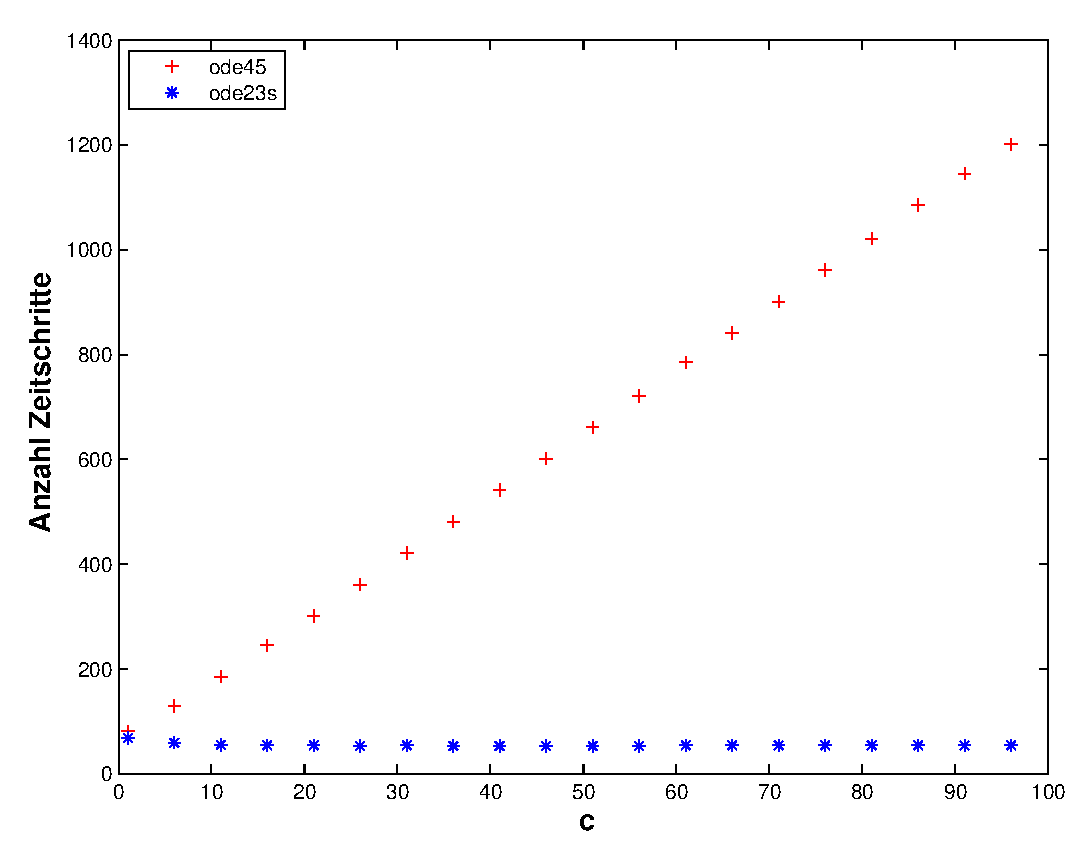
\includegraphics[width=0.9\textwidth]{../Problems/ch_ode/PICTURES/stiffrotpend.eps}
      \caption{Subproblem \ref{sp:numofsteps}: number of steps used by standard \matlab{} integrators in relation to the parameter $c$.}
        \label{fig:a3}
    \end{figure}
    
\begin{solution}
In the plot, we see that, for the solver \texttt{ode45}, the number of steps rises with $c$. On the other hand, \texttt{ode23s} uses roughly the same amount of steps, irregardless of the value of $c$ chosen.

As \texttt{ode45} is an explicit solver, it suffers under stability-based step-size limits for large $c>0$. The implicit solver \texttt{ode23s} must however not take smaller step-sizes to satisfy the tolerance for big $c$. In other words: the problem becomes stiffer, the greater the parameter $c$ is. This is expected from what we saw above.
\end{solution}
\end{subproblem}

\begin{subproblem}[2]\label{sp:4}
Formulate the non-linear equation given by the implicit mid-point rule
for the initial value problem \eqref{eq:awp3}.

\begin{solution}
With the formula for the implicit mid-point rule
    \begin{equation*}
      \Vy_{k+1} = \Vy_k + h\Vf\left(\frac{\Vy_{k} + \Vy_{k+1}}{2}\right)
    \end{equation*}
    the formulation of \eqref{eq:awp3} is given as
    \begin{equation*}
      \frac{ \Vy_{k+1} - \Vy_{k}}{h} = \Va\times\left(\frac{\Vy_k+\Vy_{k+1}}{2}\right) +
      c\left(\frac{\Vy_k+\Vy_{k+1}}{2}\right)\times\left(\Va\times\left(\frac{\Vy_k+\Vy_{k+1}}{2}\right)\right)
    \end{equation*}
\end{solution}
\end{subproblem}

\begin{subproblem}[2]
Solve \eqref{eq:awp3} with $\Va=[1,0,0]^\top$, $c=1$ up to $T=10$. Use the implicit mid-point rule and the class developed for \ref{prb:implicit_RK} with $N=128$ timesteps (use the template \texttt{cross\_template.cpp}).  Tabulate $\norm{\Vy_k}_2$ for the sequence of approximate states generated by the implicit midpoint method. What do you observe?
\begin{solution}
See file \texttt{cross.cpp}. As expected from \ref{sp:existence}, the norm of the approximate states is constant.
\end{solution}
\end{subproblem}

\begin{subproblem}[3] \label{sp:lin-imp-mpr}
The linear-implicit mid-point rule can be obtained
by a simple linearization of the incremental equation of the implicit mid-point rule around the current solution value.

Give the defining equation of the linear-implicit mid-point rule for the general autonomous differential equation
  \begin{gather*}
    \dot{\Vy} = \Vf(\Vy)
  \end{gather*}
  with smooth $f$.
  
\begin{solution}
The linear implicit mid-point rule is obtained by developing the increment $\Vk_1$ of the implicit mid point rule by its Taylor series
    \begin{align*}
      \Vk_1 = f \left(\Vy_k+\frac{h}{2}\Vk_1\right)
      = \Vf(\Vy_k) + \frac{h}{2}D\Vf(\Vy_k)\Vk_1 + O(h^2)
    \end{align*}
    and only taking the linear terms. Since the non-linear method is given by $\Vy_{k+1} = \Vy_k + h\Vk_1$, the linearization reads
    \begin{align*}
       \Vy_{k+1} = \Vy_k + h\Vk_1^{\text{lin.}}, \qquad  \Vk_1^{\text{lin.}} :=
      \left(I-\frac{h}{2}D\Vf(\Vy_k)\right)^{-1}\Vf(\Vy_k).
    \end{align*}
\end{solution}
\end{subproblem}

\begin{subproblem}[3]\label{sp:solve}
Implement the linear--implicit midpoint rule using the template provided in \texttt{cross\_template.cpp}.
Use this method to solve \eqref{eq:awp3} with $\Va=[1,0,0]^\top$, $c=1$ up to $T=10$ and $N=128$. Tabulate $\norm{\Vy_k}_2$ for the sequence of approximate states generated by the linear implicit midpoint method. What do you observe?
\begin{solution}
See file \texttt{cross.cpp}. The sequence of the norms is not exactly constant: this is due to the approximation introduced with the linearization.
\end{solution}
\end{subproblem}
\end{problem}


%%%%%%%%%%%%%%%%%%%%%%%%%%%%%%%%%%%%%%%%%%%%%%%%%%%%%%%%%%%%%%%%%%%%%%%%%%


 \begin{problem}[Semi-implicit Runge-Kutta SSM\coreproblem]\label{prb:sirk-ssm}
  General implicit Runge-Kutta methods as introduced in \lref{ss:IRK} entail
  solving systems of non-linear equations for the increments, see
  \lref{rem:stagenewton}. Semi-implicit Runge-Kutta single step methods, also
  known as Rosenbrock-Wanner (ROW) methods \lref{eq:sirkinc} just require the solution
  of linear systems of equations. This problem deals with a concrete ROW method,
  its stability and aspects of implementation.

  We consider the following  autonomous ODE
\begin{align}
 \dot{\vec{y}} = \vec{f}(\vec{y})
\end{align}
and discretize it with a \emph{semi-implicit} Runge-Kutta SSM (\emph{Rosenbrock method}):
\begin{gather} \label{method:rosenbrock}
  \begin{aligned}
    \vec{W} \vec{k}_1 & = \vec{f}(\vec{y}_0) \\
    \vec{W} \vec{k}_2 & = \vec{f}(\vec{y}_0 + \frac{1}{2} h \vec{k}_1) - a h \vec{J} \vec{k}_1 \\
    \vec{y}_1 & = \vec{y}_0 + h \vec{k}_2
  \end{aligned}
\end{gather}
where
\begin{align*}
 \vec{J} = D\vec{f}(\vec{y}_0) \\
 \vec{W} = \vec{I} - ah \vec{J} \\
 a = \frac{1}{2+\sqrt{2}}.
\end{align*}

% Cf. \cite{} as an extra reading.

\begin{subproblem}[2]
 Compute the stability function $S$ of the Rosenbrock method \eqref{method:rosenbrock}, that is, compute the (rational) function $S(z)$, such that
 \begin{align*}
  y_1 = S(z) y_0, \quad z := h \lambda,
 \end{align*}
 when we apply the method to perform one step of size $h$, starting from $y_0$, of the linear scalar model ODE $\dot{y} = \lambda y, \lambda \in \IC$.

 \begin{solution}
  For a scalar ODE, the Jacobian is just the derivative w.r.t. $y$, whence $J = D f(y) = f'(y) = (\lambda y)' = \lambda$. The quantity $\vec{W}$ is, therefore, a scalar quantity as well:
  \begin{align*}
   W = 1 - a h J = 1 - a h \lambda
  \end{align*}
  If we plug everything together and assume $h$ is small enough:
  \begin{align*}
   y_1 & = y_0 + h \frac{\vec{f}(\vec{y}_0 + \frac{1}{2} h \vec{k}_1) - a h \vec{J} \vec{k}_1}{W} \\
   & = y_0 + h \frac{\vec{f}(\vec{y}_0 + \frac{1}{2} h \frac{\vec{f}(\vec{y}_0)}{W}) - a h \vec{J} \frac{\vec{f}(\vec{y}_0)}{W})}{W} \\
   & = y_0 + h \frac{\lambda (\vec{y}_0 + \frac{1}{2} h \frac{\lambda \vec{y}_0}{1 - a h \lambda}) - \frac{a h \lambda^2 y_0}{1 - a h \lambda}}{1 - a h \lambda} \\
   & = \frac{(1 - a h \lambda)^2 + h \lambda (1 - a h \lambda) + \frac{1}{2} h^2 \lambda^2 - a h^2 \lambda^2}{(1 - a h \lambda)^2} y_0 \\
   & = \frac{(1 + a^2 z^2 - 2az) + z (1 - a z) + \frac{1}{2} z^2 - a z^2}{(1 - a z)^2} y_0 \\
   & = \frac{1 + (1-2a) z +  (\frac{1}{2}-2a+ a^2) z^2}{(1 - a z)^2} y_0
  \end{align*}
  Since $\frac{1}{2}-2a+ a^2 = 0$, it follows
  \begin{align*}
   S(z) = \frac{1 + (1-2a) z}{(1 - a z)^2}
  \end{align*}
 \end{solution}
\end{subproblem}

\begin{subproblem}[3]
 Compute the first $4$ terms of the Taylor expansion of $S(z)$ around $z = 0$. What is the maximal $q \in \IN$ such that
 \begin{align*}
  \lvert S(z) - \exp(z) \rvert = O(\lvert z \rvert^q)
 \end{align*}
 for $\lvert z \rvert \rightarrow 0$? Deduce the maximal possible 
 order of the method \eqref{method:rosenbrock}.
 
 \begin{hint}
   The idea behind this sub-problem is elucidated in \lref{rem:stabexp}. Apply
   \lref{lem:Sapproxexp}. 
 \end{hint}

 \begin{solution}
  We compute:
  \begin{align*}
   S(0) & = 1, \\
   S'(0) & = 1, \\
   S''(0) & = 4a - 2 a^2, \\
   S'''(0) & = 18a^2 - 12a^3,
  \end{align*}
   therefore
   \begin{align*}
    S(z) = 1 + z + (2a - a^2) z^2 + (3a^2 - 2a^3) z^3 + O(z^4).
   \end{align*}
  We can also compute the expansion of $\exp$:
   \begin{align*}
    \exp(z) = 1 + z + \frac{1}{2} z^2 + \frac{1}{6} z^3 + O(z^4)
   \end{align*}
   and since $2a - a^2 = \frac{1}{2}$ but $3a^2 - 2a^3 = \frac{1}{2}(\sqrt{2}-1) \neq \frac{1}{6}$, we have:
 \begin{align*}
  \lvert S(z) - \exp(z) \rvert = O(\lvert z \rvert^3)
 \end{align*}
 Using \ncseref{lem:Sapproxexp}, we deduce that the maximal order $q$ of the scheme is $q = 2$.
 \end{solution}
\end{subproblem}

\begin{subproblem}[2]
 Implement a \Cpp{} function:
\begin{lstlisting}[language=c++]
template <class Func, class DFunc, class StateType>
std::vector<StateType> solveRosenbrock(
		      const Func & f, const DFunc & df,
		      const StateType & y0,
		      unsigned int N, double T)
 \end{lstlisting}
 taking as input function handles for $\vec{f}$ and $D\vec{f}$ (e.g. as lambda
 functions), an initial data (vector or scalar) \verb|y0| $= \vec{y}(0)$, a number
 of steps $N$ and a final time $T$. The function returns the sequence of states generated
 by the single step method up to $t = T$, using $N$ equidistant steps of the
 Rosenbrock method \eqref{method:rosenbrock}.
 
 \cprotEnv \begin{hint}
  See \verb|rosenbrock_template.cpp|.
 \end{hint}
 
 \cprotEnv \begin{solution}
  See \verb|rosenbrock.cpp|.
 \end{solution}
\end{subproblem}

\begin{subproblem}[3]
 Explore the order of the method \eqref{method:rosenbrock} empirically by applying it to the IVP for the limit cycle \ncseref{ex:limitcycle}:
 \begin{align}
  \vec{f}(\vec{y}) := \begin{bmatrix}
                       0 & -1 \\ 1 & 0
                      \end{bmatrix} \vec{y} + \lambda ( 1 - \lVert \vec{y} \rVert^2 ) \vec{y},
 \end{align}
 with $\lambda = 1$ and initial state $\vec{y_0} = [1,1]^\top$ on $[0,10]$. Use fixed timesteps of size $h = 2^{-k}, k = 4,\dots,10$ and compute a reference solution with $h = 2^{-12}$ step size. Monitor the maximal mesh error:
 \begin{align*}
  \max_j \lVert  \vec{y}_j - \vec{y}(t_j) \rVert_2.
 \end{align*}
 \cprotEnv \begin{solution}
  The Jacobian $Df$ is:
  \[
  D\vec{f}(\vec{y}) = \begin{bmatrix}
                       \lambda ( 1 - \lVert \vec{y} \rVert^2 ) - 2 \lambda y_0^2 & -1 -2 \lambda y_1 y_0 \\
                       1 -2 \lambda y_1 y_0 & \lambda ( 1 - \lVert \vec{y} \rVert^2 ) - 2 \lambda y_1^2
                      \end{bmatrix}.
  \]
  For the implementation, cf. \verb|rosenbrock.cpp|.
 \end{solution}
\end{subproblem}

\begin{subproblem}[4]
 Show that the method \eqref{method:rosenbrock} is $L$-stable (cf. \ncseref{par:Lstab}).
 \begin{hint}
To investigate the $A$-stability, calculate the complex norm of $S(z)$ on the imaginary axis $\Re{z}=0$ and apply the following maximum principle for holomorphic functions:

\begin{theorem}[Maximum principle for holomorphic functions]
 Let \[\IC^- := \{ z \in \IC \; | \; Re(z) < 0 \}.\] Let $f: D \subset \IC \rightarrow \IC$ be non-constant, defined on $\overline{\IC^-}$, and analytic in $\IC^-$. Furthermore, assume that $w := \lim_{ \lvert z \rvert \rightarrow \infty} f(z)$ exists and $w \in \IC$, then:
 \begin{align*}
  \forall z \in \IC^- \lvert f(z) \rvert < \sup_{\tau \in \IR} \lvert f(i \tau) \rvert.
 \end{align*}
\end{theorem}
 \end{hint}

 \begin{solution}
  We start by proving that the method is $A$-stable \ncseref{par:Astab}, meaning that $S(z) < 1, \forall z \in \IC, \mathrm{Re}(z) < 0$. First of all, we can compute the complex norm of the stability function at $z = iy, y \in \IR$ as:
  \begin{align*}
   \lvert S(iy) \rvert^2 = \frac{\lvert 1 + (1-2a) iy \rvert^2}{\lvert(1 - a iy)^2 \rvert^2} = \frac{1+ (1-2a)^2y^2}{(1+ a^2 y^2)^2} = \frac{1+ (1-4a+4a^2)y^2}{(1+ 2a^2 y^2 + a^4 y^4)}.
  \end{align*}
  Notice that $1 - 4a + 4a^2 = 2a^2$, therefore:
  \begin{align*}
   \lvert S(iy) \rvert^2 = \frac{1+ 2 a^2 y^2}{1+ 2a^2 y^2 + a^4 y^4} < 1.
  \end{align*}
  The norm of the function $S$ is bounded on the imaginary axis. Observe that $\lvert S(z) \rvert \rightarrow 0, \lvert z \rvert \rightarrow \infty$, which, follows from the fact that the degree of the denominator of $S$ is bigger than the polynomial degree of the numerator.
  Notice that $1-2a = 1-2\frac{1}{\sqrt(2)+2} = \sqrt{2} - 2$.
  
  The only pole of the function is at $z = 1/a$, therefore the function is holomorphic on the left complex plane.
  
  Applying the theorem of the hint on concludes that the absolute value of the function is bounded by $1$ on the left complex plane.
  
  The $L$-stability follows immediately with $A$-stability and the fact that the absolute value of the function converges to zero as $\lvert z \rvert \rightarrow \infty$.
 \end{solution}
\end{subproblem}


 
\end{problem}
 
 \begin{problem}[Singly Diagonally Implicit Runge-Kutta Method]\label{prb:sdirk} 
  SDIRK-methods (\textbf{S}ingly \textbf{D}iagonally
  \textbf{I}mplicit \textbf{R}unge-\textbf{K}utta methods) are distinguished by
  Butcher schemes of the particular form
  \begin{gather}
    \label{eq:BSexpl}
    \begin{array}[c]{c|c}
      \Vc & \FA \\\hline
          & \Vb^{T}
    \end{array} \quad:= \quad
    \arraycolsep=1.4pt\def\arraystretch{2.2}
    \begin{array}[c]{c|cccccc}
      c_{1} & \gamma  & & & \cdots & & 0 \\
      c_{2} & a_{21} & \ddots &&&& \vdots \\
      \vdots & \vdots &&&& \ddots & \vdots \\
      c_{s} & a_{s1} && \cdots & & a_{s,s-1} & \gamma \\\hline
            & b_{1} && \cdots && b_{s-1} & b_{s}
    \end{array}\;,
\end{gather}  
with \Blue{$\gamma\not=0$}. 

More concretely, in this problem the scalar linear initial value problem of second
order
\begin{equation} \label{eq:awp}
  \ddot{y} + \dot{y} + y = 0,
  \qquad
  y(0)=1,
  \quad
  \dot{y}(0) = 0
\end{equation}
should be solved numerically using a SDIRK-method (\textbf{S}ingly \textbf{D}iagonally
\textbf{I}mplicit \textbf{R}unge-\textbf{K}utta Method).
It is a Runge-Kutta method described by the Butcher scheme
\begin{gather}\label{eq:1}
  \begin{array}{c|cc}
    \gamma & \gamma & 0 \\
    1-\gamma & 1-2\gamma & \gamma \\\hline
    & 1/2 & 1/2\rule{0pt}{2.2ex}
  \end{array}.
\end{gather}
%

\begin{subproblem}[1]\label{sp:0}
  Explain the benefit of using SDIRK-SSMs compared to using Gauss-Radau RK-SSMs as
  introduced in \lref{ex:RADAU}. In what situations will this benefit matter much? 

  \begin{hint}
    Recall that in every step of an implicit RK-SSM we have to solve a non-linear
    system of equations for the increments, see \lref{rem:stagenewton}. 
  \end{hint}
\end{subproblem}

\begin{subproblem}[1]\label{sp:1}
State the equations for the increments $\vec{k}_{1}$ and $\vec{k}_{2}$ of the Runge-Kutta method \eqref{eq:1} applied to the initial value problem corresponding to the differential equation $\displaystyle \dot{\By} = \Vf(t,\By)$.

\begin{solution}
The increments $\Bk_i$ are given by
\begin{align*}
	\Bk_1 &= f\left(t_0 + h\gamma, \By_0 + h\gamma\Bk_1\right),\\
	\Bk_2 &= f\left(t_0 + h(1-\gamma), \By_0 + h(1-2\gamma)\Bk_1 + h\gamma\Bk_2\right).
\end{align*}
\end{solution}

\end{subproblem}

\begin{subproblem}[1]\label{sp:2}
Show that, the stability function $S(z)$ of the SDIRK-method \eqref{eq:1} is given by
\begin{equation*}
S(z) = \frac{1 + z(1 - 2\gamma) + z^2(1/2 - 2\gamma + \gamma^2)}{(1-\gamma z)^2}
\end{equation*}
and plot the stability domain using the template \texttt{stabdomSDIRK.m}.

For $\gamma=1$ is this method:
\begin{itemize}
	\item A--stable?
	\item L--stable?
\end{itemize}
\begin{hint}
Use the same theorem as in the previous exercise.
\end{hint}

\begin{solution}
The stability function $S(z)$ of a method is derived by applying the method to the scalar, linear test equation
\begin{equation*}
	\dot{y}(t) = \lambda y(t)
\end{equation*}
The solution can be written as
\begin{equation*}
	y_{k+1} = S(z)y_k
\end{equation*}
where $S(z)$ is the stability function and $z:= h\lambda$.

In the case of the SDIRK-method, we get
\begin{align*}
	k_1 &= \lambda(y_k + h\gamma k_1)\qquad \\
	k_2 &= \lambda(y_k + h(1-2\gamma)k_1 + h\gamma k_2),
\end{align*}
therefore
\begin{align*}
	k_1 &= \frac{\lambda}{1 - h\lambda\gamma}y_k,\\
	k_2 &= \frac{\lambda}{1 - h\lambda\gamma}(y_k + h(1-2\gamma)k_1).
\end{align*}
Furthermore
\begin{equation*}
	y_{k+1} = y_k + \frac{h}{2}(k_1 + k_2),
\end{equation*}
with $z:= h\lambda$ and by plugging in $k_1$ and $k_2$ we arrive at
\begin{equation*}
	y_{k+1} = \underbrace{\left(1 + \frac{z}{2(1-\gamma z)}\left(2 + \frac{z(1-2\gamma)}{1-\gamma z}\right)\right)}_{=: S(z)}y_k.
\end{equation*}
Hence
\begin{align*}
	S(z) &= \frac{2(1-\gamma z)^2 + 2z(1-\gamma z)^2 + z^2(1-2\gamma)}{2(1-\gamma z)^2}
	\intertext{
and after collecting the powers of $z$ in the numerator we get
	}
	S(z) &= \frac{1 + z(1-2\gamma) + z^2(\gamma^2 - 2\gamma + \frac{1}{2})}{(1-\gamma z)^2}.
\end{align*}
For $\gamma=1$ the stability function is therefore
\begin{equation} \label{eq:stabfun1}
	S_1(z) := \frac{1 - z - \frac{z^2}{2}}{(1-z)^2}.
\end{equation}

\textbf{Verification of the A-stability of \eqref{eq:stabfun1}:}\\
By definition \ncseref{par:Astab},  we need to show that $|S_1(z)| \le 1$ for all  $z\in\bbC^-:= \{ z \in \bbC \; | \;  \Re z < 0 \}$.
In order to do this we consider the stability function on the imaginary axis
\begin{align*}
	|S_1(i y)|^2 &= \frac{|1 - i y - (i y)^2/2|^2}{|1-i y|^4}\\
	&= \frac{|1 -i y + y/2|^2}{|1-i y|^4}\\
	&= \frac{(1+y^2/2)^2 + y^2}{(1+y^2)^2}\\
	&= \frac{1 + 2y^2 + y^4/4}{1 + 2y^2 + y^4} \le 1,\quad y\in\bbR.
\end{align*}
Since the only pole ($z=1$) of the rational function $S_1(z)$ lies in the positive half plane of $\bbC$, the function $S_1$ is holomorphic in the left half plane. Furthermore $S_1$ is bounded by 1 on the boundary of this half plane (i.e. on the imaginary axis). So by the maximum principle for holomorphic functions (hint) $S_1$ is bounded on the entire left half plane by 1. This implies in particular that $S_1$ is $A$-stable.
% (see Ahlfors, \emph{Complex Analysis} or Conway, \emph{Functions of One Complex Variable}).

\textbf{Verification of the L-stability of \eqref{eq:stabfun1}:}\\
$S_1$ is not $L$-stable (cf. definition \ncseref{par:Lstab}), because
\begin{equation*}
	\lim_{\Re z\to -\infty} |S_1(z)| = \lim_{\Re z\to-\infty} \left|\frac{1-z-z^2/2}{1-2z+z^2}\right| = \frac{1}{2} \ne 0.
\end{equation*}

\end{solution}
\end{subproblem}

\begin{subproblem}[1] \label{sp:3}
Formulate \eqref{eq:awp} as an initial value problem for a linear first order system for the function $\Bz(t) = (y(t),\dot{y}(t))^\top$.

\begin{solution}
Define $z_1=y$, $z_2=\dot{y}$, then the initial value problem
\begin{equation}\label{eq:awp2}
	\ddot{y} + \dot{y} + y = 0,\qquad y(0)=1,\quad \dot{y}(0) = 0
\end{equation}
is equivalently to the first order system
\begin{align}\label{eq:system}
	\dot{z}_1 &= z_2 \notag\\
	\dot{z}_2 &= -z_1 -z_2,
\end{align}
with initial values $z_1(0)=1$, $z_2(0)=0$.
\end{solution}

\end{subproblem}

\begin{subproblem}[1]\label{sp:4}
Implement a \Cpp{}-function
\begin{lstlisting}[language=c++]
template <class StateType>
StateType sdirtkStep(const StateType & z0, double h, double gamma);
\end{lstlisting}
that realizes the numerical evolution of one step of the method \eqref{eq:1} for the differential equation determined in \autoref{sp:3} starting from the value \verb|z0| and returning the value of the next step of size \verb|h|.

\begin{hint}
See \verb|sdirk_template.cpp|.
\end{hint}

\cprotEnv \begin{solution}
Let
\[
	\VA:=\left(\begin{array}{c c}0&1\\-1&-1\end{array}\right).
\]
Then
\begin{align*}
k_1&= \VA \By_0+h\gamma\VA k_1\\
k_2&= \VA\By_0+h(1-2\gamma)\VA k1+h\VA k_2,
\end{align*}
so
\begin{align*}
k_1&= (\VI-h\gamma\VA)^{-1} \VA \By_0\\
k_2&= (\VI-h\gamma\VA)^{-1}(\VA\By_0+h(1-2\gamma)\VA k_1).
\end{align*}
See the implementation in \verb|sdirk.cpp|.
% \lstinputlisting[ emph={sdirkStep}, caption={Perform one iteration of \eqref{eq:1}},
%                   label={code:sdirkStep}]{matlab/sdirkStep.m}
% }
\end{solution}

\end{subproblem}

\begin{subproblem}[1]\label{sp:5}
  Use your \Cpp{} code to conduct a numerical experiment, which gives an
  indication of the order of the method (with $\gamma=\frac{3+\sqrt{3}}{6}$) for
  the initial value problem from \autoref{sp:3}.  Choose $\By_0=[1,0]^\top$ as
  initial value, \texttt{T=10} as end time and \texttt{N=20,40,80,\dots,10240} as
  steps.
	
\cprotEnv \begin{solution}
The numerically estimated order of convergence is $3$, see \verb|sdirk.cpp|.
\end{solution}
\end{subproblem}
	
% \lstinputlisting[ emph={sdirkConv}, caption={Calculate the order of convergence of \eqref{eq:1} },
%                   label={code:sdirkConv}]{matlab/sdirkConv.m}
% \end{solution}
% \begin{center}
%   \begin{math}
%     \label{eq:sdirk1}
%     \begin{tabular}{c|cc}
%       $\gamma$ & $\gamma$ & $0$ \\
%       $1-\gamma$ & $1-2\gamma$ & $\gamma$ \\\hline
%       & $1/2$ & $1/2$
%     \end{tabular}
%   \end{math}
% \end{center}
% \end{subproblem}
%%%%%%%%%%%%%%%%%%%%%%%%%%%%%%%%%%%%%%%%%%%%%%%%%%%%%%%%%%%%%%%%%%%%%%%%%

\end{problem}
%{\small
%\lstinputlisting[ emph={}, caption={Testcalls for \autoref{prb:sdirk}},
   %               label={code:test_call}]{matlab/test_call.m}

%\lstinputlisting[ emph={}, caption={Output for Testcalls for \autoref{prb:sdirk}},
   %               label={code:test_call_out}]{matlab/test_call_out.txt}
%}

\end{sheet}


\printbibliography

\end{document}
